\documentclass{article}

% Formatting
\DeclareUnicodeCharacter{2060}{\nolinebreak} % Prevent unicode (U+2060) error on local complile
\frenchspacing % No double spacing between sentences
\hbadness=1000000 % Turn off \hbox badness warnings
\linespread{1.2} % Set linespace


% Packages
\usepackage[a4paper, left=1.5cm, right=1.5cm, top=2.0cm, bottom=2.0cm]{geometry}
\usepackage{authblk} % For author formatting
\usepackage{caption} % For figure and table captions
\usepackage{cclicenses} % For creative commons license
\usepackage{float} % To force figure location after text
\usepackage{graphicx} % Adds more functionality to graphics for inclusion of figures
%\usepackage{hyperref} % For clickable web links
\usepackage{lscape} % For landscape pages
\usepackage{lineno} % Allows use of \linenumbers to add line numbers 
\usepackage{lmodern} % A scalable font - avoids erros due to non-sclabale fonts
\usepackage{longtable,booktabs}  % For tables
\usepackage{makecell} % For cell formatting in tables
\usepackage{markdown} % allow use of markdown syntax
\usepackage{microtype} % 'Improved' typesetting
\usepackage[nottoc]{tocbibind} % Add references to table of contents
\usepackage{parskip} % Adds white space between paragraphs
\usepackage{pdflscape} % To create landscape pages that show as landscape in PDF viewer
\usepackage{ragged2e} % Better right ragged edges (allows hyphenation)
\usepackage{subcaption} % Allows use of subfigures
\usepackage[super]{natbib} % Citations using superscript
\usepackage{titlesec} % For title spacing
\usepackage[toc,page]{appendix}
\usepackage{url} % Tidy web links
\usepackage[utf8]{inputenc}
\usepackage{verbatim}
\usepackage{xcolor} % For coloured text
\usepackage{xurl} % For url but with more flexible linebreaking
\usepackage{placeins} % to use \FloatBarrier where want a hard break between content (to force and order of text and figures
\usepackage[hidelinks]{hyperref}


% Info on wordcounts:
% https://www.overleaf.com/learn/how-to/Is_there_a_way_to_run_a_word_count_that_doesn%27t_include_LaTeX_commands%3F

% To include refs in word count:
%TC:incbib

\newcommand{\detailtexcount}[1]{%
  \immediate\write18{texcount -merge -sum -q #1.tex output.bbl > #1.wcdetail }%
  \verbatiminput{#1.wcdetail}%
}

% Count tables in wordcount (change to 0 0 if tables not included in word count)
%TC:group table 0 1
%TC:group tabular 1 

%%%%%%%% Compile mode %%%%%%%%
% Choose what to compile by setting \compilemode:
%   1 = main paper only (no supplement)
%   2 = supplement only
%   3 = everything (main paper + supplement)
\newcommand{\compilemode}{3}

\newif\ifincludemain
\newif\ifincludesupplement
\ifcase\compilemode
  \or \includemaintrue  \includesupplementfalse % 1: main only
  \or \includemainfalse \includesupplementtrue  % 2: supplement only
  \or \includemaintrue  \includesupplementtrue  % 3: everything
  \else \errmessage{compilemode must be 1, 2 or 3}
\fi

% Abstract: choose length
% Use \shortabstracttrue for the ~300-word abstract,
% or \shortabstractfalse for the ~500-word abstract
\newif\ifshortabstract
\shortabstracttrue

% Number for supplementary material
\newcommand{\beginsupplement}{
    \setcounter{section}{0}
    \renewcommand{\thesection}{S\arabic{section}}
    \setcounter{figure}{0}
    \renewcommand{\thefigure}{S\arabic{figure}}
    \setcounter{table}{0}
    \renewcommand{\thetable}{S\arabic{table}}
}


\begin{document}

% Ignore title and abstract in word count
%TC:ignore
\title{Timing of thrombolysis and thrombectomy and outcome in patients with acute ischaemic stroke arriving within six hours of onset: an observational study of national registry data}


\renewcommand{\thefootnote}{\fnsymbol{footnote}}

% Order to be decided
\author[*1,2]{Michael Allen}
\author[1,2]{Anna Laws}
\author[1,2]{Yinghui Wei}
\author[1,2]{Kerry Pearn}
\author[4]{Peter McMeekin}
\author[3]{Richard Everson}
\author[3]{Mark Kelson}
\author[4]{Jason Scott}
\author[4]{Eleanor Kashouris}
\author[1]{Joao Delgado}
\author[1,2]{Leon Farmer}
\author[1,2]{Lauren Asare}
\author[5]{Ajay Bhalla}
\author[1,2]{Martin James}

% Check affiliations - update RDE Name
\affil[1]{\footnotesize University of Exeter Medical School}
\affil[2]{\footnotesize NIHR South West Applied Research Collaboration (ARC).}
\affil[3]{\footnotesize University of Exeter}
\affil[4]{\footnotesize University of Northumbria}
\affil[5]{\footnotesize Guys and St Thomas NHS Foundation Trust}
\affil[6]{\footnotesize Royal Devon University Healthcare NHS Foundation Trust}
\affil[*]{\footnotesize Corresponding author: m.allen@exeter.ac.uk}

\date{}
\maketitle

\ifincludemain
% ---------------------------------------------------------------------------
% Abstract: two versions (approx. 300 and 500 words).
% Choose which is used with the switch in main.tex:
%   \shortabstracttrue   -> ~300-word abstract
%   \shortabstractfalse  -> ~500-word abstract
% ---------------------------------------------------------------------------

\section*{Abstract}

\ifshortabstract
% ======================= ~300-word abstract =======================

\textbf{Background:} Intravenous thrombolysis (IVT) and mechanical thrombectomy (MT) are both time-dependent, but randomised trials have largely studied each in isolation. In routine care, many patients receive IVT at one hospital and MT, sometimes hours later, at another. We estimated the real-world effectiveness of IVT and MT, alone and combined, and how it depends on the timing of each.

\textbf{Methods:} We used national stroke registry data for 74,678 patients with ischaemic stroke and an NIHSS score above 5 (or a recorded large vessel occlusion) who arrived within six hours of onset at MT-performing hospitals in England and Wales, 2020--2025. A good outcome was a discharge modified Rankin Scale (mRS) score of 0--2, or no worse than before the stroke. We used three causal methods with different assumptions: target trial emulation by matching, an explainable S-learner, and an orthogonal causal forest. Treatment was classed as early ($\leq$270 minutes from onset) or late.

\textbf{Results:} 28,884 patients received IVT alone, 2,983 MT alone and 5,164 both. Every strategy improved outcomes, and all three methods ranked them identically. Early combined treatment gave the largest benefit: 46\% of treated patients versus 24\% of matched controls had a good outcome (causal forest: about 18 percentage points). Early MT alone and early IVT alone gave gains of about 14 and 10 percentage points. Benefit declined approximately linearly with delay, reaching zero at about 6.8 hours for IVT and 9.9 hours for MT; each hour of delay multiplied the odds ratio by about 0.84 (IVT) and 0.86 (MT). Early IVT added most when MT was delayed.

\textbf{Conclusions:} In routine practice, IVT and MT are each effective, with time dependence closely matching the trials. The greatest benefit comes from giving both treatments early; stroke services should aim to minimise both treatment times, not either alone.

\else
% ======================= ~500-word abstract =======================

\textbf{Background:} Intravenous thrombolysis (IVT) and mechanical thrombectomy (MT) are highly effective stroke treatments, but the benefit of each declines with delay. Trials have largely studied each treatment and its timing in isolation, and trials of MT with or without prior IVT recruited patients in whom the two treatments were given close together. In routine care, many patients receive IVT locally and are transferred for MT, which may follow hours later. We estimated the real-world effectiveness of IVT and MT, alone and combined, and how it depends on the time to each treatment, separately and together.

\textbf{Methods:} We used data from the Sentinel Stroke National Audit Programme (SSNAP) for 74,678 patients with ischaemic stroke and an NIHSS score above 5 (or a recorded large vessel occlusion) who arrived within six hours of known onset at MT-performing hospitals in England and Wales between 2020 and 2025. A good outcome was a discharge modified Rankin Scale (mRS) score of 0--2, or no worse than before the stroke. Treatment was classed as early ($\leq$270 minutes from onset) or late ($>$270 minutes). We used three causal inference methods with different assumptions: target trial emulation by matching; an explainable S-learner (XGBoost), predicting each patient's outcome with and without treatment; and an orthogonal, doubly robust causal forest. Effects were estimated in treated patients. A secondary model with SHAP explanations identified the characteristics associated with greater benefit.

\textbf{Results:} Overall, 28,884 patients received IVT alone, 2,983 MT alone, 5,164 both, and 37,647 neither. Every strategy was associated with a higher chance of a good outcome, and all three methods ranked the strategies identically. Early combined treatment gave the largest benefit: 46\% of treated patients against 24\% of matched controls had a good outcome, the S-learner estimated an odds ratio of about 4.4, and the causal forest an absolute gain of about 18 percentage points. Early MT alone and early IVT alone gave absolute gains of about 14 and 10 percentage points. Late treatments gave roughly half to two thirds of the benefit, on the log odds scale, of their early counterparts, and patients receiving early IVT with late MT gained little more than those receiving early IVT alone. With treatment times modelled continuously, benefit declined approximately linearly, reaching zero at about 6.8 hours for IVT and 9.9 hours for MT; each hour of delay multiplied the odds ratio by about 0.84 (IVT) and 0.86 (MT). Joint analysis showed that benefit was greater the earlier IVT was given, for any time to MT, and the earlier MT followed, for any time to IVT. The admitting stroke team, stroke severity and pre-stroke disability were most associated with the size of benefit.

\textbf{Conclusions:} In routine practice, IVT and MT are each effective, with benefits and time dependence closely matching the randomised trials. Early IVT adds substantially to MT, especially when MT is delayed, whereas MT adds little to early IVT once delayed beyond about six hours. The greatest benefit comes from giving both treatments early, and services should minimise both treatment times, not either alone.

\fi

\fi
%TC:endignore

%%%%%%%% Main paper
\ifincludemain

\newpage

\section{Introduction}

% Burden of stroke

Stroke remains one of the top three global causes of death and disability, accounting for 10.7\% of all deaths globally and 5.7\% of lost disability-adjusted life-years (DALYs) \cite{feigin_global_2021}. Despite reductions in age-standardised rates of stroke, ageing populations are driving an increase in the absolute number of strokes \cite{feigin_global_2021}. Across Europe, in 2017, stroke was found to cost healthcare systems \texteuro 27 billion, or 1.7\% of health expenditure \cite{luengo-fernandez_economic_2020}. The burden is increasing; it has been estimated that the number of stroke survivors aged 45 and over in the UK will more than double between 2015 and 2035 \cite{king_future_2020}.

% IVT

Intravenous thrombolysis (IVT) with alteplase was established by randomised trials showing benefit when given within 3 hours of onset \cite{ninds1995}, a window later extended to 4.5 hours \cite{hacke2008}. The individual patient data meta-analysis of Emberson et al., pooling 6{,}756 patients from nine trials, quantified how strongly that benefit depends on time \cite{emberson_effect_2014}. The odds of an excellent outcome (a modified Rankin Scale [mRS] score of 0--1 at 3--6 months) were increased by 75\% when treatment was given within 3 hours (OR 1.75, 95\% CI 1.35--2.27) and by 26\% between 3 and 4.5 hours (OR 1.26, 95\% CI 1.05--1.51), with no significant benefit beyond 4.5 hours (OR 1.15, 95\% CI 0.95--1.40). In absolute terms, this corresponds to roughly ten additional patients per 100 treated achieving an excellent outcome if treated within 3 hours, falling to about five per 100 between 3 and 4.5 hours. Alteplase increased the risk of fatal intracranial haemorrhage in the first week by about 2 percentage points, a risk that did not diminish with later treatment, so the balance of benefit and harm worsens as time passes. IVT can be delivered at any acute stroke unit with access to brain imaging, but it is relatively ineffective at recanalising large, proximal clots.

% MT

Mechanical thrombectomy (MT) is suitable for patients with large vessel occlusion (LVO) of the anterior circulation, who account for a minority of ischaemic strokes but a disproportionate share of death and severe disability. The HERMES collaboration pooled individual data on 1{,}287 patients from five trials and found that MT substantially reduced disability at 90 days (OR 2.49, 95\% CI 1.76--3.53), with functional independence (mRS 0--2) in 46.0\% of treated patients against 26.5\% of controls, and a number needed to treat of 2.6 for one patient to improve by at least one mRS level \cite{goyal2016}. This makes MT one of the most effective interventions in acute medicine.

As with IVT, the effect diminishes with delay. In the MR CLEAN trial, Fransen et al.\ found that the absolute benefit of MT on functional independence fell by about 6 percentage points for every hour of delay to reperfusion, from an estimated 25.9\% with reperfusion at 3 hours to 6.7\% at 6 hours \cite{fransen_time_2016}. The HERMES time-to-treatment meta-analysis confirmed the pattern across trials: each hour of delay to reperfusion was associated with worse disability (common OR 0.84, 95\% CI 0.76--0.93), and the benefit of MT over IVT was no longer statistically significant beyond 7.3 hours from onset \cite{saver2016}. Later trials showed that patients selected by advanced imaging can still benefit up to 24 hours after they were last known to be well \cite{nogueira2018,albers2018}, but these patients are a selected subgroup, and earlier treatment remains better for them too.

% Aims of project
The evidence above treats the two treatments, and the two treatment times, largely in isolation. The alteplase trials relate benefit to time to IVT in populations for whom MT was not available \cite{emberson_effect_2014}, and the MT trials relate benefit to time to reperfusion in patients, most of whom had already received alteplase, without modelling when the alteplase was given \cite{goyal2016,saver2016}. Trials comparing MT with and without prior IVT recruited patients presenting directly to MT centres, in whom the interval between the two treatments was short and varied little \cite{majoie2023,kaesmacher2024}.

In routine practice, the two times vary independently: many patients receive IVT at their local hospital and are then transferred for MT, which may follow one or several hours later. It is therefore unclear how much each treatment adds to the other at a given pair of treatment times. It is also uncertain how well trial estimates, obtained in selected patients, describe the benefit achieved in the wider population treated in routine care.
 
Large national registries offer a means of addressing these questions, but treatment in routine care is not randomised, and those treated differ systematically from those who are not. Target trial emulation, in which the analysis of observational data is designed to mirror the trial that would ideally have been run, combined with modern causal machine learning methods, allows treatment effects to be estimated from such data under explicit assumptions \cite{hernan2016}.
 
The aim of this study was to estimate the real-world effectiveness of IVT and MT, alone and in combination, in patients with ischaemic stroke and an NIHSS score above 5 (or a recorded large vessel occlusion) arriving at hospital within six hours of stroke onset, using national registry data from England and Wales. Specifically, we set out to:
 
\begin{enumerate}
    \item estimate the effect of IVT, MT, and their combination on disability at discharge, compared with no reperfusion treatment;
    \item describe how that effect depends on the time from onset to each treatment, considering time to IVT and time to MT both separately and jointly;
    \item assess the robustness of these estimates by applying three causal inference methods with differing assumptions (target trial emulation by matching, an explainable S-learner, and a causal forest), and by comparing the results with those of the randomised trials where such trials exist;
    \item identify the patient and service characteristics that most influence the benefit gained from treatment.
\end{enumerate}
\section{Patients and methods}

\subsection{Data and patients}

We used anonymised data from the Sentinel Stroke National Audit Programme (SSNAP), the national stroke registry for England and Wales, for admissions in 2020--2025 (Healthcare Quality Improvement Partnership data request HQIP515). SSNAP is a prospective national audit that records the care and outcomes of patients admitted to hospital with stroke, in order to measure and improve stroke services against national standards; it includes over 90\% of stroke admissions, and each hospital's completeness and timeliness of data entry are scored and published. We included patients with ischaemic stroke who arrived within 6 hours of known onset and had an NIHSS score above 5 or a recorded LVO. We excluded patients without a recorded discharge modified Rankin Scale (mRS) score, with recorded use of perfusion imaging, who received IVT 6 hours or more or MT 12 hours or more after onset, or who were recorded as receiving IVT after MT. Of the 74,678 patients included, 28,884 received IVT alone, 2,983 MT alone, 5,164 both, and 37,647 neither (patient flow diagrams are given in Supplementary Figures~\ref{fig:flow_tte}--\ref{fig:flow_cf}). Patients were first admitted by 116 stroke teams, each with at least 10 eligible patients who received MT, at that hospital or after transfer.

\subsection{Treatment groups and outcome}

Patients were grouped by the reperfusion treatment they received (IVT alone, MT alone, or both) and its timing, with each treatment classed as early ($\leq$270 minutes from onset) or late ($>$270 minutes). A good outcome was a discharge mRS of 0--2, or no worse than before the stroke, so that patients with pre-stroke disability who returned to their previous level of function had a good outcome.  Discharge mRS was recorded in routine care by hospital staff, without blinding to treatment. All three methods estimated the effect of treatment in the patients who received it (the average treatment effect in the treated, ATT), compared with no reperfusion treatment.

\subsection{Causal inference methods}

We used three causal inference methods resting on different assumptions; full descriptions and a study protocol for each method are given in Supplementary Sections~\ref{sec:supp_methods} and~\ref{sec:protocol}. The protocol was written during the analysis and was not registered in advance; later additions are identified in it.

\textit{Target trial emulation by matching.} The analysis was designed to mirror the randomised trial that would ideally have been run \cite{hernan2016}. For each treatment group, every treated patient was matched to an untreated patient with the same pre-stroke mRS, 5-year age band, 5-point NIHSS band (0--4, 5--9, 10--14, \textit{et seq.}), atrial fibrillation (AF) diagnosis and anticoagulant use for AF \cite{stuart2010matching}. Each untreated patient could be used as a control up to three times. The proportion with a good outcome was compared between treated patients and their matched controls.

\textit{S-learner.} A single machine learning model (XGBoost \cite{chen_xgboost_2016}) predicted each patient's chance of a good outcome from their characteristics, stroke team and the treatment received, with treatment represented either by the actual onset-to-treatment times (with a treatment not given coded as an arbitrarily long time) or by the early/late groups. Each treated patient's benefit was the difference between their predicted outcome with the treatment received and with that treatment removed \cite{kunzel2019metalearners}. Predictions came from models that had not seen the patient (five-fold cross-validation), and confidence intervals came from repeating the whole procedure on 30 bootstrap samples. Missing values (NIHSS in 67 patients) were left as missing and handled by XGBoost's built-in method, which learns at each split which branch missing values should follow, so no patients were excluded. A second model, explained with SHAP values \cite{shap_documentation}, identified the characteristics associated with greater benefit.

\textit{Causal forest.} A causal forest within a double machine learning framework \cite{chernozhukov2018double,wager2018estimation} first predicted each patient's outcome and their likely treatment from their characteristics, stroke team and year of admission, and then estimated treatment effects from the variation that these predictions could not explain. Effects in the treated were estimated by augmented inverse-probability weighting. This approach is doubly robust: its estimates remain unbiased if either the outcome model or the treatment model is correct. Onset-to-scan time was not adjusted for in the primary analysis, because it largely determines whether early treatment is possible: adjusting for it compares early-treated patients with untreated patients who were also scanned early, many of whom will have had a specific reason not to be treated. Its influence was instead tested in a sensitivity analysis. The 67 patients with missing data were excluded.

\subsection{Sensitivity analyses}

For each method, we repeated the analysis changing one choice at a time: the early/late cut-off, the definition of a good outcome, the characteristics used for matching or adjustment (including comorbidities, LVO, stroke team and onset-to-scan time) and model settings. We assessed unmeasured confounding with E-values, the minimum strength of association that a hidden confounder would need with both treatment and outcome to explain away an effect \cite{vanderweele2017evalue}, and with the sensemakr method of Cinelli and Hazlett, which compares such a confounder with measured characteristics such as stroke severity \cite{cinelli2020sensemakr}. To show how much each estimate depended on the strongest measured confounders, we also repeated each analysis leaving out stroke severity, age or pre-stroke disability in turn (Supplementary Section~\ref{sec:supp_loo}).

\subsection{Code availability}

All code and results are available at \url{https://github.com/samuel-book/samuel-3}.
\section{Results}

\subsection{Patients}

Patients who received MT, with or without IVT, had more severe strokes and less pre-stroke disability than those who received IVT alone, and those who received MT alone were far more likely to have AF and to be taking anticoagulants (Table~\ref{tab:matching}). Matching produced closely balanced groups, and at most 2.6\% of any group could not be matched, although diabetes, and to a lesser extent hypertension, were less common in patients given MT than in their matched controls (these comorbidities were not used for matching; see Sensitivity analyses).

{\small
\begin{longtable}[]{@{}llll@{}}
\caption{Characteristics of treated patients and their matched untreated controls in the target trial emulation, by treatment strategy. Values are mean (standard deviation); for yes/no characteristics the mean is the proportion of patients. $n$: matched treated patients. Early: $\leq$270 minutes from onset; late: $>$270 minutes. Patients were matched on pre-stroke disability, age band, NIHSS band, AF diagnosis and anticoagulant use for AF; each control could be used for up to three treated patients.}\\
\toprule
\textbf{Treatment group} & \textbf{Feature} & \textbf{Treated} & \textbf{Untreated} \\
\midrule
\endfirsthead
\multicolumn{4}{@{}l}{\textit{Table \thetable\ continued}}\\
\endhead
\endlastfoot
Early IVT only (n=27536) & Pre-stroke mRS & 1.00 (1.31) & 1.00 (1.31) \\
& NIHSS score & 12.58 (6.11) & 12.52 (6.17) \\
& Age & 74.28 (13.28) & 74.28 (13.28) \\
& Congestive heart failure & 0.05 (0.23) & 0.06 (0.23) \\
& Hypertension & 0.55 (0.50) & 0.56 (0.50) \\
& Diabetes & 0.21 (0.41) & 0.24 (0.43) \\
& Anticoagulant for AF & 0.03 (0.18) & 0.03 (0.18) \\
& AF diagnosis & 0.21 (0.41) & 0.21 (0.41) \\
Late IVT only (n=1183) & Pre-stroke mRS & 0.97 (1.29) & 0.97 (1.29) \\
& NIHSS score & 11.89 (5.89) & 11.82 (5.96) \\
& Age & 73.93 (13.22) & 73.93 (13.22) \\
& Congestive heart failure & 0.06 (0.23) & 0.05 (0.22) \\
& Hypertension & 0.57 (0.50) & 0.57 (0.50) \\
& Diabetes & 0.23 (0.42) & 0.25 (0.43) \\
& Anticoagulant for AF & 0.03 (0.18) & 0.03 (0.18) \\
& AF diagnosis & 0.20 (0.40) & 0.20 (0.40) \\
Early MT only (n=1078) & Pre-stroke mRS & 0.75 (0.89) & 0.75 (0.89) \\
& NIHSS score & 17.75 (5.88) & 17.59 (6.13) \\
& Age & 73.14 (12.65) & 73.14 (12.65) \\
& Congestive heart failure & 0.11 (0.31) & 0.09 (0.29) \\
& Hypertension & 0.54 (0.50) & 0.58 (0.49) \\
& Diabetes & 0.17 (0.38) & 0.25 (0.43) \\
& Anticoagulant for AF & 0.53 (0.50) & 0.53 (0.50) \\
& AF diagnosis & 0.58 (0.49) & 0.58 (0.49) \\
Late MT only (n=1840) & Pre-stroke mRS & 0.62 (0.84) & 0.62 (0.84) \\
& NIHSS score & 15.89 (5.96) & 15.69 (6.17) \\
& Age & 72.51 (13.19) & 72.51 (13.19) \\
& Congestive heart failure & 0.07 (0.26) & 0.08 (0.27) \\
& Hypertension & 0.53 (0.50) & 0.56 (0.50) \\
& Diabetes & 0.18 (0.38) & 0.22 (0.42) \\
& Anticoagulant for AF & 0.39 (0.49) & 0.39 (0.49) \\
& AF diagnosis & 0.47 (0.50) & 0.47 (0.50) \\
Early IVT + Early MT (n=2288) & Pre-stroke mRS & 0.42 (0.74) & 0.42 (0.74) \\
& NIHSS score & 17.26 (5.89) & 17.10 (6.16) \\
& Age & 69.66 (13.00) & 69.66 (13.00) \\
& Congestive heart failure & 0.04 (0.20) & 0.04 (0.20) \\
& Hypertension & 0.47 (0.50) & 0.51 (0.50) \\
& Diabetes & 0.14 (0.34) & 0.22 (0.41) \\
& Anticoagulant for AF & 0.03 (0.16) & 0.03 (0.16) \\
& AF diagnosis & 0.23 (0.42) & 0.23 (0.42) \\
Early IVT + Late MT (n=2688) & Pre-stroke mRS & 0.40 (0.73) & 0.40 (0.73) \\
& NIHSS score & 16.13 (6.02) & 15.93 (6.19) \\
& Age & 70.48 (13.45) & 70.48 (13.45) \\
& Congestive heart failure & 0.04 (0.20) & 0.05 (0.21) \\
& Hypertension & 0.51 (0.50) & 0.51 (0.50) \\
& Diabetes & 0.16 (0.37) & 0.21 (0.41) \\
& Anticoagulant for AF & 0.03 (0.17) & 0.03 (0.17) \\
& AF diagnosis & 0.24 (0.43) & 0.24 (0.43) \\
Late IVT + Late MT (n=141) & Pre-stroke mRS & 0.45 (0.70) & 0.45 (0.70) \\
& NIHSS score & 15.06 (6.03) & 14.93 (6.37) \\
& Age & 70.20 (13.50) & 70.20 (13.50) \\
& Congestive heart failure & 0.05 (0.22) & 0.02 (0.14) \\
& Hypertension & 0.48 (0.50) & 0.55 (0.50) \\
& Diabetes & 0.25 (0.43) & 0.17 (0.38) \\
& Anticoagulant for AF & 0.04 (0.20) & 0.04 (0.20) \\
& AF diagnosis & 0.17 (0.38) & 0.17 (0.38) \\
\bottomrule
\label{tab:matching}
\end{longtable}
}

\subsection{Effect of each treatment strategy}

Every treatment strategy was associated with a higher chance of a good outcome (Table~\ref{tab:effects}). All three methods found that early IVT plus early MT gave the largest benefit: 46.5\% of treated patients had a good outcome against 23.0\% of matched controls, the S-learner odds ratio was 3.2 (log odds ratio 1.16), and the causal forest estimated a gain of 15.2 percentage points. Early MT alone gave the next largest benefit, followed by early IVT alone. The causal forest gave smaller gains than matching for the three early strategies, but similar gains for the late strategies. In the S-learner, late treatment gave about half to two thirds of the benefit of early treatment on the log odds scale, and early IVT followed by late MT gave no more than early IVT alone. Only 141 patients received both treatments late, and their estimates were imprecise.

\begin{table}[htbp]
\centering
\caption{Estimated effect of each treatment strategy on a good outcome at discharge (mRS 0--2, or no worse than before the stroke), by method. Early: $\leq$270 minutes from onset; late: $>$270 minutes. Target trial emulation: percentage with a good outcome in treated patients and matched controls, and the difference (percentage points), with 95\% confidence intervals. S-learner: mean log odds ratio, treated \textit{vs} untreated (95\% CI from 30 bootstrap refits of the model); a log odds ratio of 0.69 corresponds to an odds ratio of 2.0, and 1.10 to 3.0. Causal forest: average treatment effect in the treated, percentage points (95\% CI); 67 patients with missing data excluded. $n$: patients in each group before matching. $^{**}p<0.01$.}
\label{tab:effects}
\resizebox{\textwidth}{!}{%
\begin{tabular}{@{}lrrrrll@{}}
\toprule
 & & \multicolumn{3}{c}{Target trial emulation} & S-learner & Causal forest \\
\cmidrule(lr){3-5}
Treatment strategy & $n$ & Treated (\%) & Control (\%) & Difference & Log odds ratio (95\% CI) & ATT, pp (95\% CI) \\
\midrule
Early IVT only & 27,695 & 49.0 (48.5--49.6) & 36.6 (36.1--37.2) & 12.4 (11.6--13.2)$^{**}$ & 0.64 (0.59--0.69)$^{**}$ & 9.9 (8.8--11.0)$^{**}$ \\
Late IVT only & 1,189 & 47.3 (44.4--50.1) & 40.9 (38.1--43.7) & 6.3 (2.3--10.3)$^{**}$ & 0.41 (0.29--0.53)$^{**}$ & 9.5 (6.5--12.5)$^{**}$ \\
Early MT only & 1,107 & 39.1 (36.1--42.0) & 21.9 (19.4--24.4) & 17.2 (13.3--21.0)$^{**}$ & 1.00 (0.86--1.14)$^{**}$ & 12.1 (7.4--16.8)$^{**}$ \\
Late MT only & 1,876 & 33.5 (31.3--35.6) & 25.2 (23.2--27.2) & 8.3 (5.3--11.2)$^{**}$ & 0.47 (0.37--0.58)$^{**}$ & 9.4 (7.1--11.7)$^{**}$ \\
Early IVT + early MT & 2,309 & 46.5 (44.5--48.5) & 23.0 (21.3--24.7) & 23.5 (20.8--26.2)$^{**}$ & 1.16 (1.05--1.27)$^{**}$ & 15.2 (10.9--19.6)$^{**}$ \\
Early IVT + late MT & 2,714 & 37.2 (35.4--39.0) & 26.2 (24.6--27.9) & 11.0 (8.5--13.4)$^{**}$ & 0.60 (0.51--0.69)$^{**}$ & 9.3 (6.8--11.7)$^{**}$ \\
Late IVT + late MT & 141 & 44.0 (35.7--52.3) & 27.0 (19.5--34.4) & 17.0 (5.9--28.1)$^{**}$ & 0.69 (0.38--0.99)$^{**}$ & 15.4 (6.6--24.2)$^{**}$ \\
\bottomrule
\end{tabular}%
}
\end{table}

\subsection{Effect of time to treatment}

Figure~\ref{fig:main_s_learner_matrix} shows the S-learner's estimated benefit by time to IVT and time to MT. The benefit of each treatment given alone declined steadily with delay, reaching zero at 406 minutes (6.8 hours; 95\% CI 402--409) for IVT and 570 minutes (9.5 hours; 563--577) for MT. The IVT figure is an extrapolation beyond the 6-hour limit for IVT in this cohort, and neither figure is a treatment time limit. For MT, each hour of delay multiplied the odds ratio for a good outcome by about 0.86. The effects of the two treatment times were not independent. For a fixed time to MT, benefit was greater the earlier IVT had been given: with MT at 240--300 minutes, the log odds ratio rose from 0.68 without IVT to 1.06 with IVT at 60--120 minutes. For a fixed time to IVT, benefit fell the later MT followed: with IVT at 60--120 minutes, it fell from 1.71 with MT at 60--120 minutes to 0.81 with MT at 360--420 minutes, close to the 0.84 for IVT alone. The benefit of early combined treatment (1.16) was less than the sum of those of early IVT alone and early MT alone (0.64 and 1.00).

\begin{figure}
    \centering
    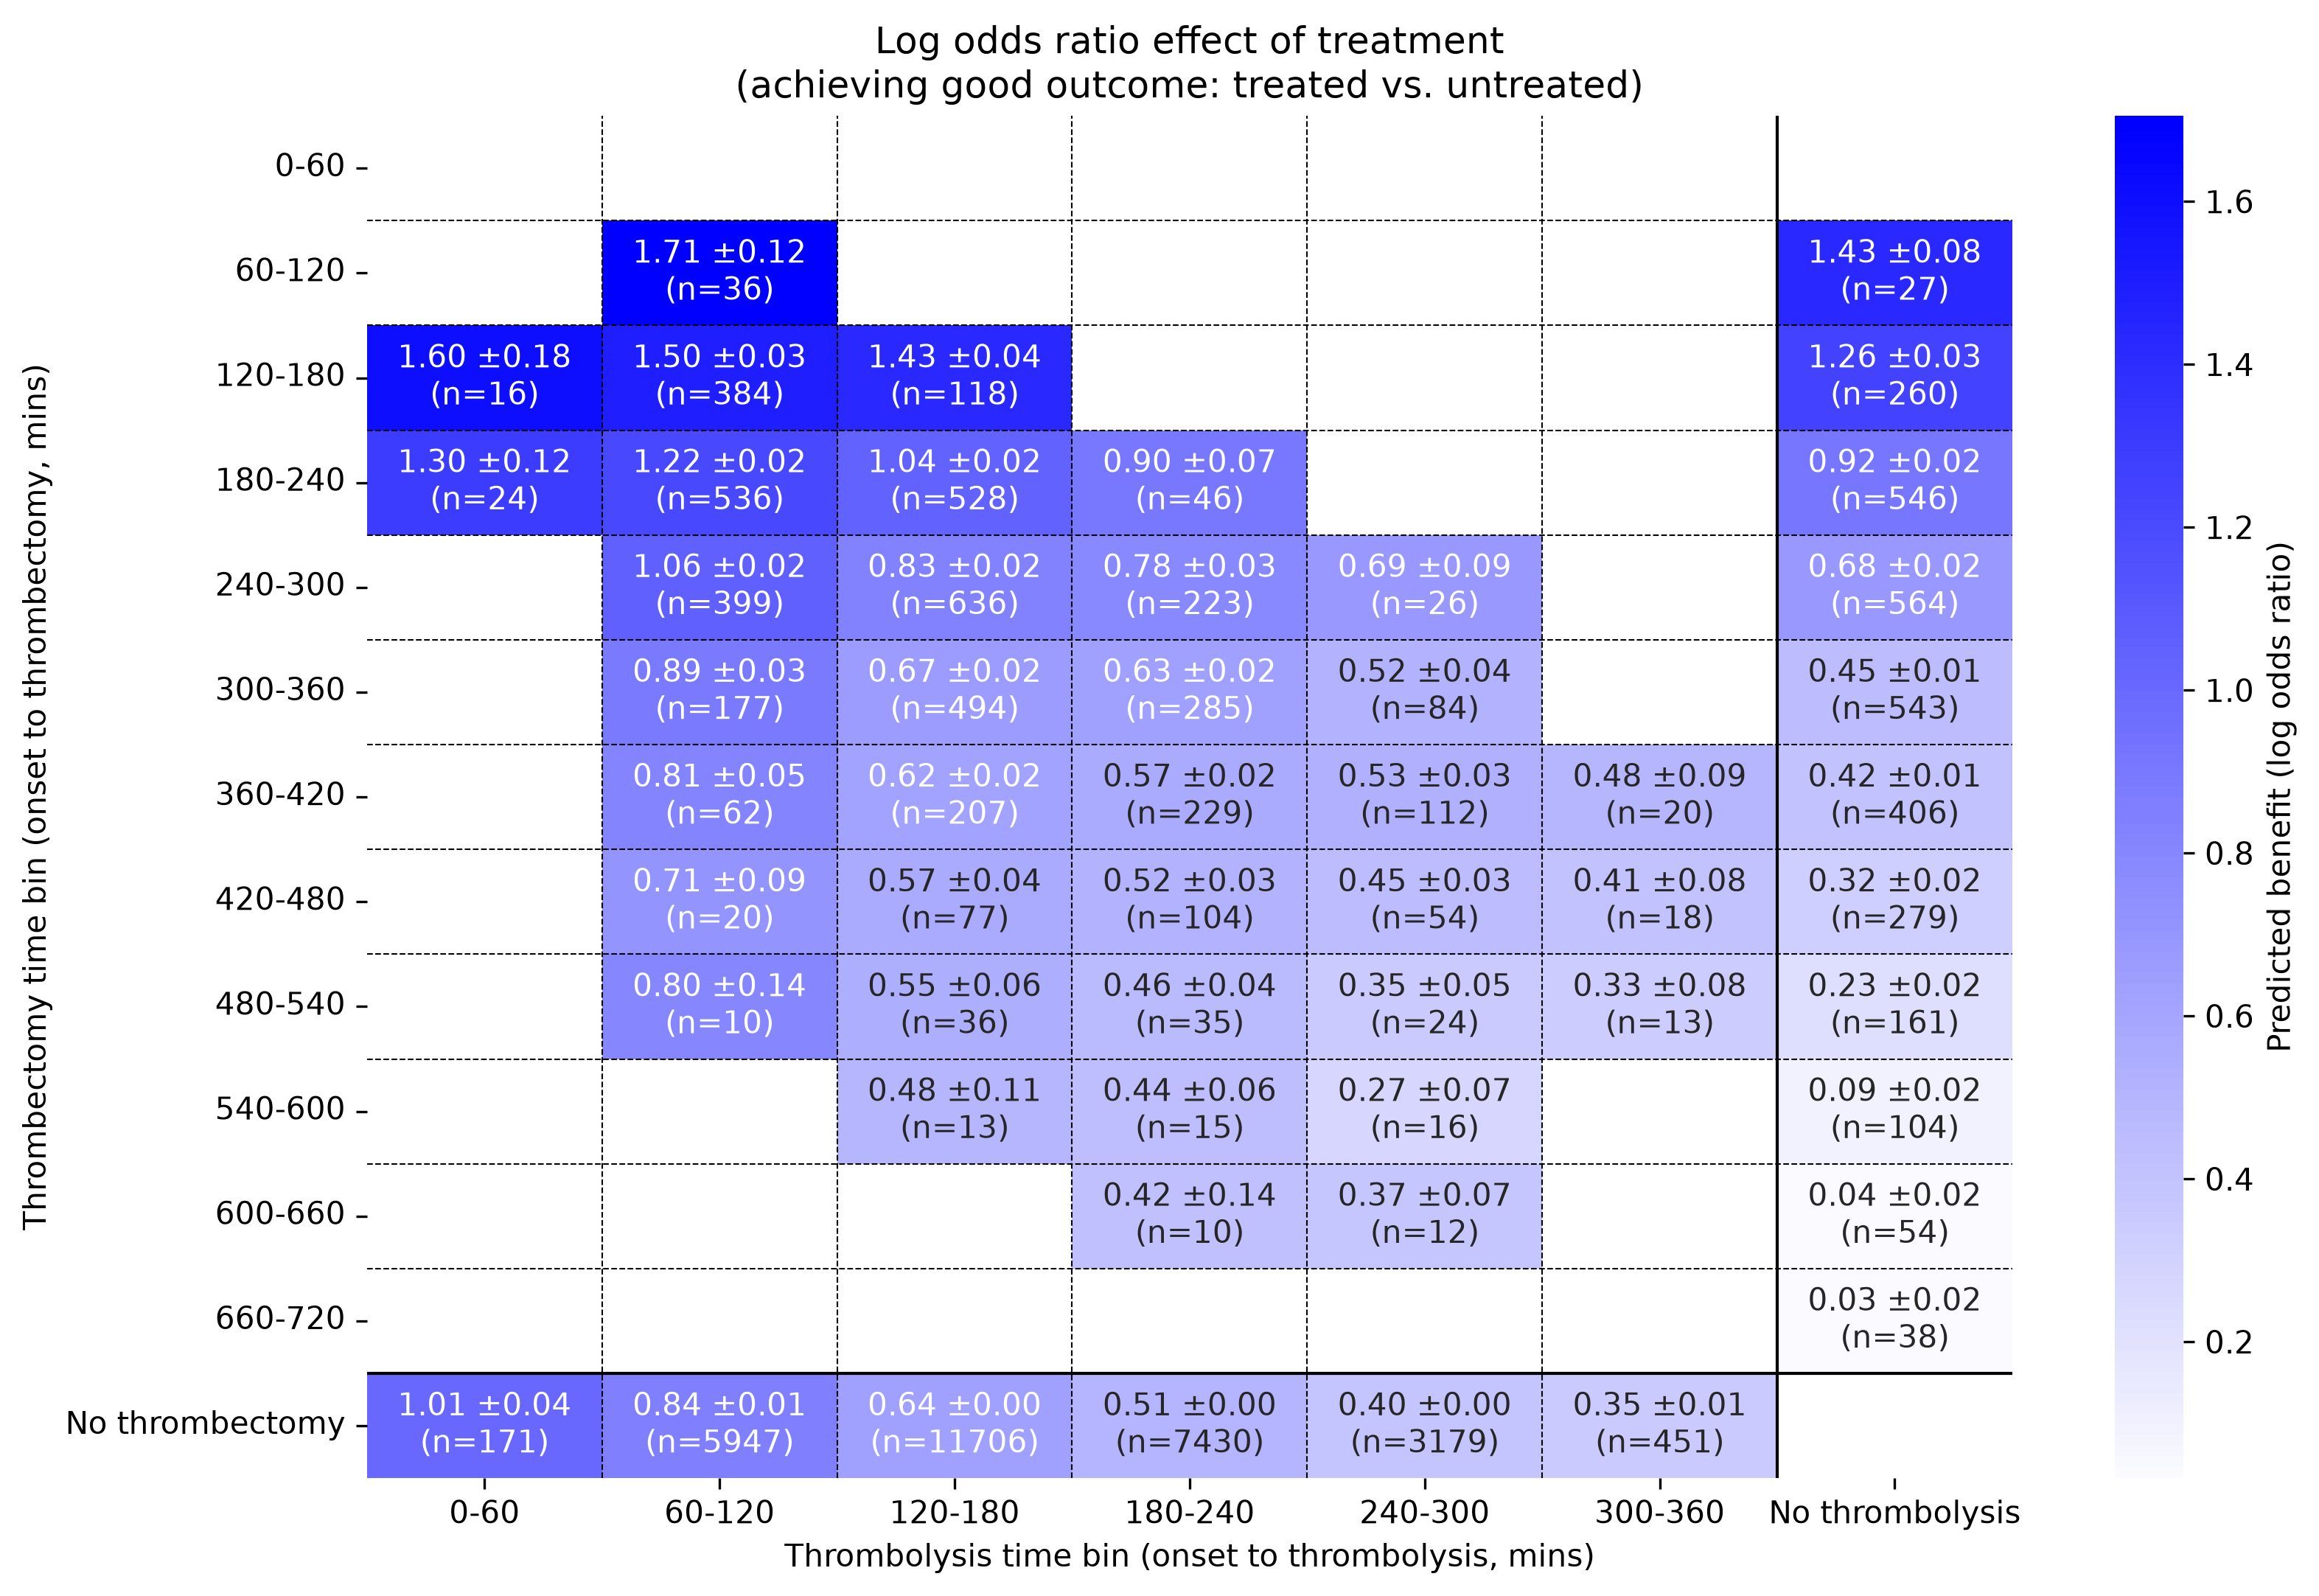
\includegraphics[width=1\linewidth]{images/treatment_effects/non_mild_stroke_early_arrival_good_outcome_s_learner_heatmap_log_odds.png}
    \caption{S-learner estimate of the benefit of treatment (log odds of a good outcome, treated \textit{vs} untreated) by onset-to-IVT time (columns) and onset-to-MT time (rows). Each cell shows the mean $\pm$ the half-width of its 95\% confidence interval (variation between patients only), with the number of patients in parentheses. The last row is IVT without MT and the last column MT without IVT; cells with fewer than 10 patients are blank.}
    \label{fig:main_s_learner_matrix}
\end{figure}

\subsection{Characteristics associated with greater benefit}

The features most associated with the size of benefit were stroke severity, the type and timing of treatment, the stroke team attended, age and pre-stroke disability (Figure~\ref{fig:main_s_learner_benefit_shap_mrs_2}). Benefit increased with stroke severity up to an NIHSS score of about 20, and was smaller with greater pre-stroke disability and in patients aged 80 or over.

\begin{figure}
    \centering
    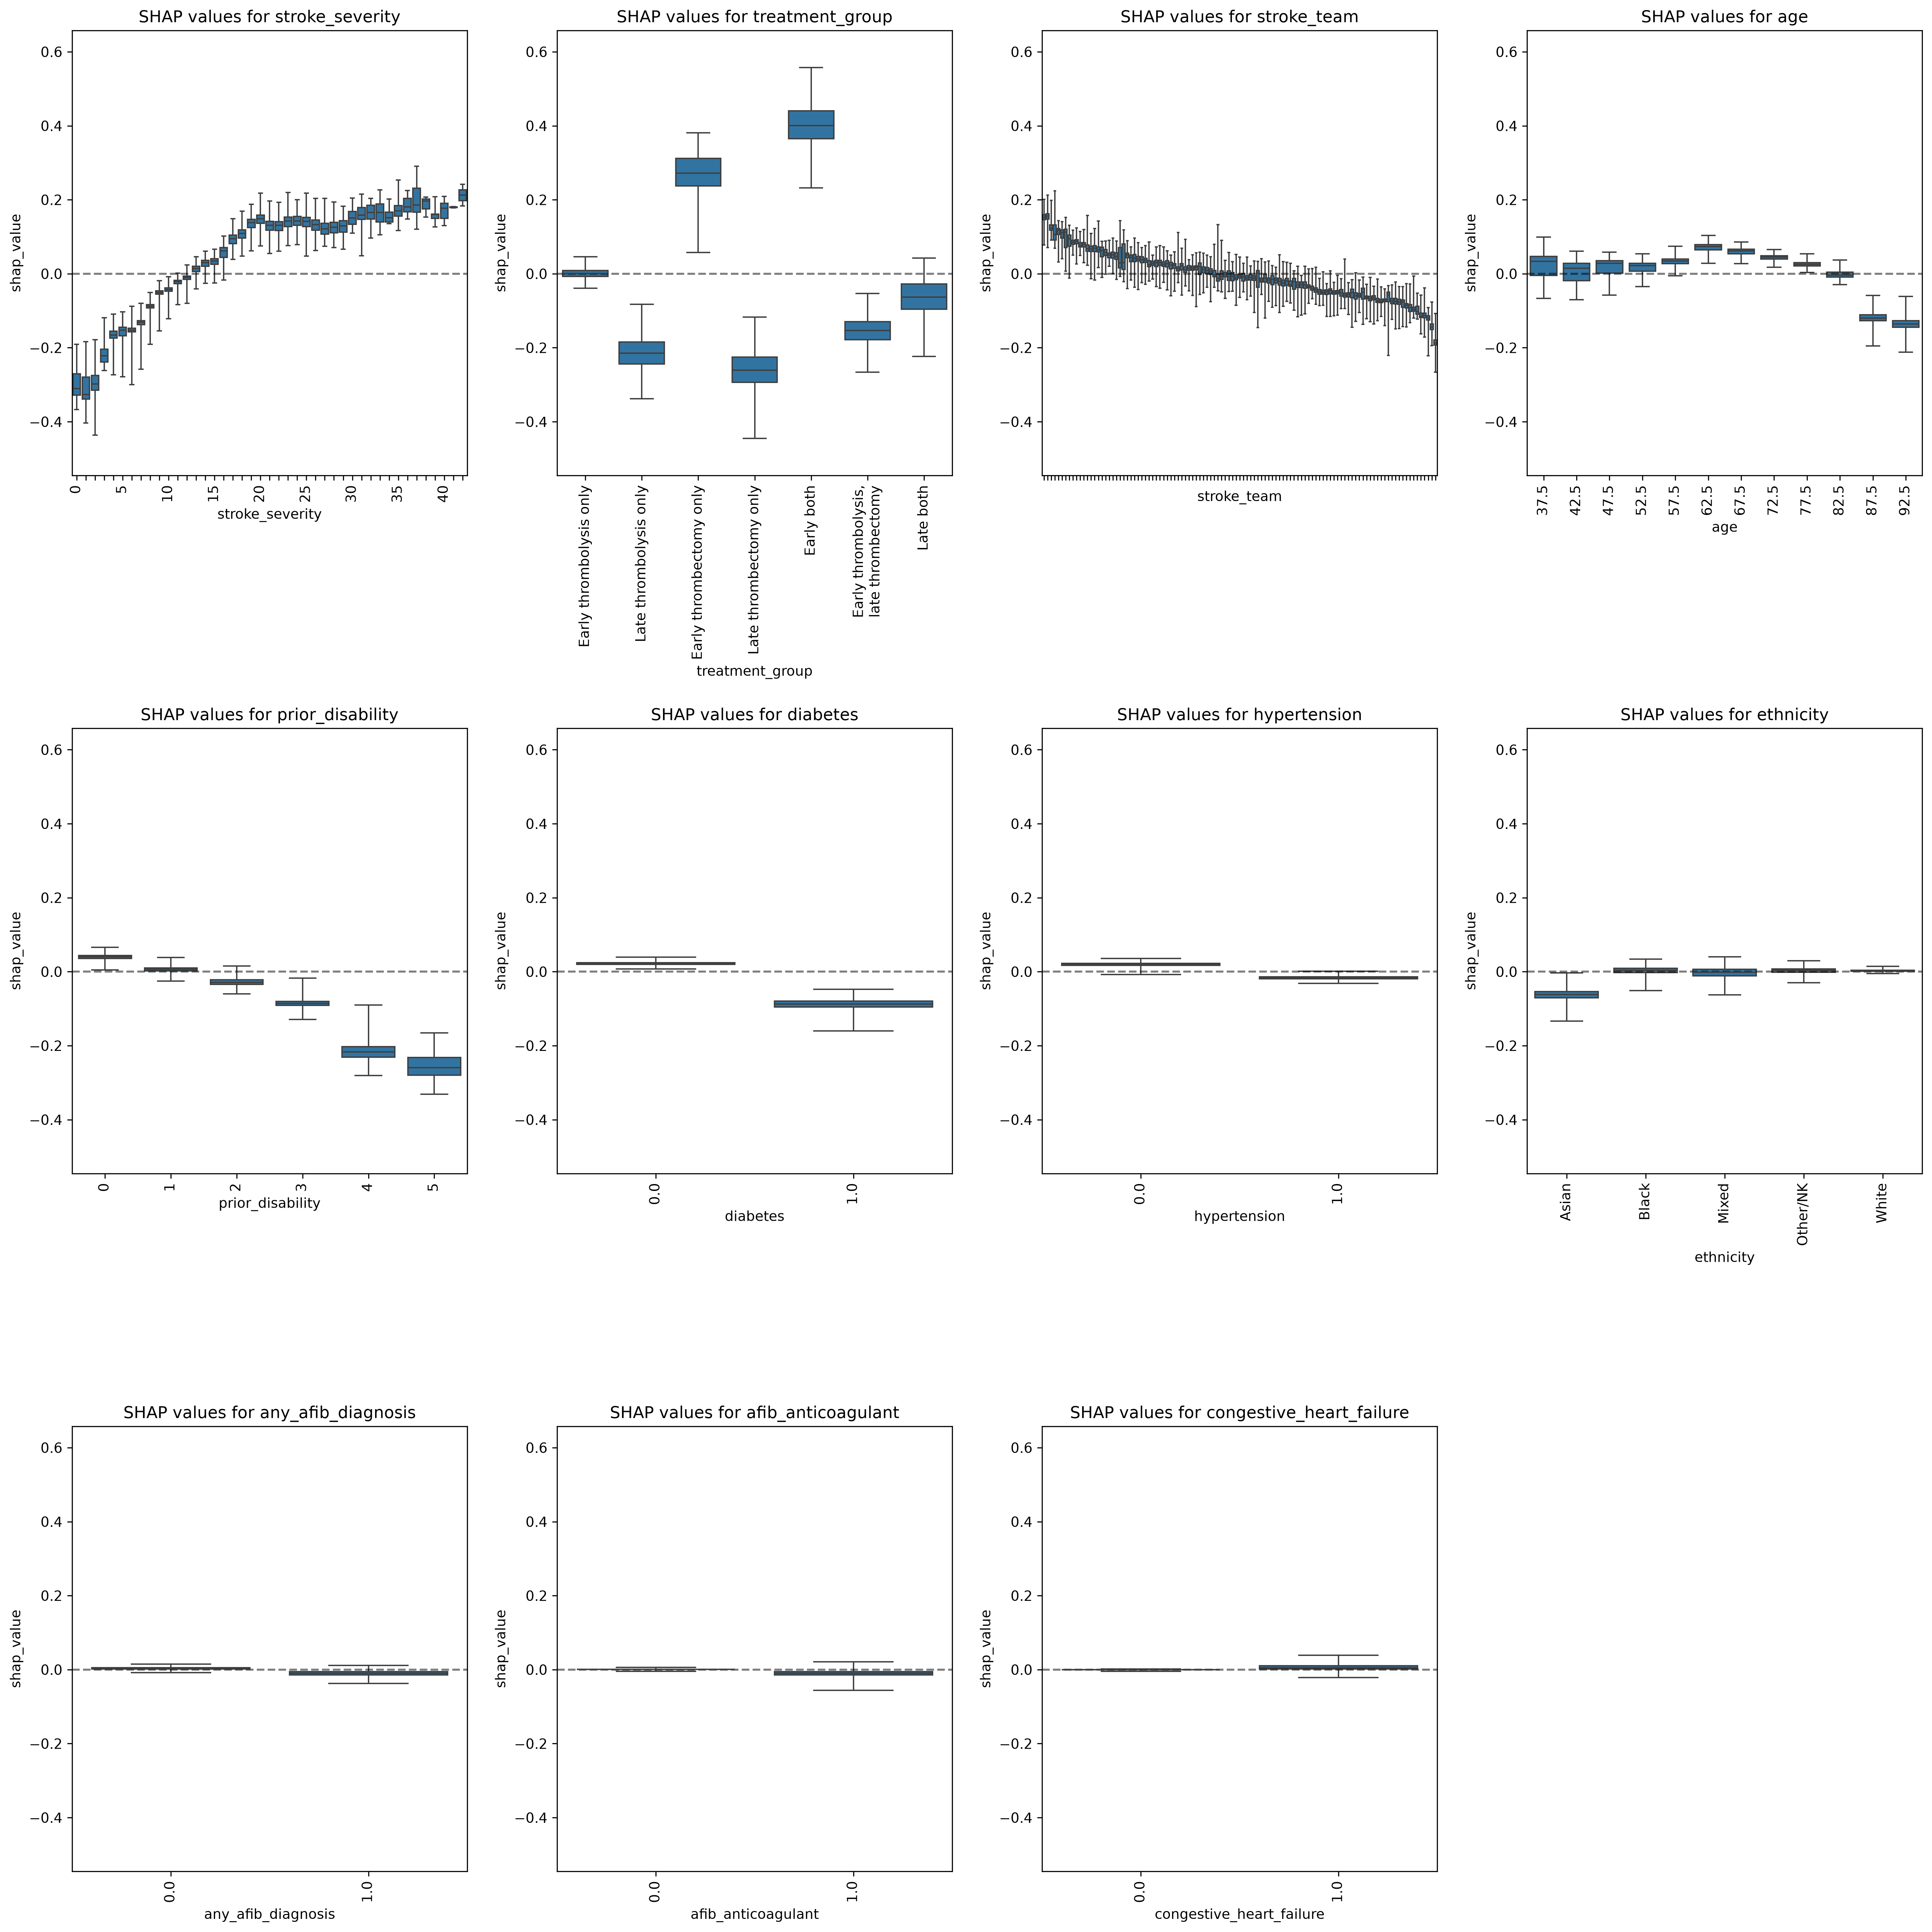
\includegraphics[width=1\linewidth]
{images/treatment_effects/non_mild_stroke_early_arrival_good_outcome_s_learner_treatment_effect_shap_box_plots.png}
    \caption{Patient characteristics associated with the predicted benefit of treatment. Each panel shows box plots of SHAP values (contribution to the log odds of a good outcome, treated \textit{vs} untreated) for each feature value; panels are ordered by average effect.}
    \label{fig:main_s_learner_benefit_shap_mrs_2}
\end{figure}

\subsection{Sensitivity analyses}

In every sensitivity analysis, each strategy remained associated with more good outcomes, mostly with changes of 3 percentage points or less (Supplementary Section~\ref{sec:sensitivity}). Adding comorbidities to the matching reduced the estimate for early MT alone from 17.2 to 12.6 percentage points, and adjusting for LVO, where recorded, increased the MT estimates. Without adjustment for onset-to-scan time and year of admission, the causal forest estimates for early treatment came within 1.5 percentage points of matching. In the S-learner and causal forest analyses, the effects of IVT alone would survive a hidden confounder three times as strong as stroke severity, age or onset-to-scan time, but one as strong as stroke severity or pre-stroke disability could remove or halve the benefit of MT. Deliberately leaving out a measured confounder gave the same picture in all three methods: without stroke severity, the MT estimates fell by 10--19 percentage points, to between $-$6 and $+$5 percentage points, whereas the IVT-alone estimates changed by 4 percentage points or less; leaving out pre-stroke disability reduced the estimates by up to 11 percentage points, and leaving out age changed them by about 3 percentage points or less (up to 6 in the 141 patients treated late with both) (Supplementary Section~\ref{sec:supp_loo}).

\section{Discussion}

\textbf{ADD DISCUSSION HERE}

Key points to cover:

\begin{itemize}

    \item We are looking at patients who receive treatment without selection by advanced imaging; this is the 'common' patients, and will show the general pattens of effectiveness.

    \item We are looking at the treatment effect in those treated. There are difference in baseline characteristics between these groups.
    
    \item All methods give substantially the same results

    \item Early combined treatment is best

   
\end{itemize}

%\section{References}
\bibliographystyle{naturemag}
%\bibliographystyle{plainnat}
%\bibliographystyle{unsrt}
%\bibliographystyle{unsrtnat}
\bibliography{references}

\fi


%%%%%%%% Supplement
\ifincludesupplement

\ifincludemain
  \clearpage
\fi
\beginsupplement % Resets numbering
\centerline{{\huge Supplementary Material}}
\section{Code}

All code used is published at \url{https://github.com/samuel-book/samuel-3}. The repository contains the data-processing, modelling and plotting code needed to reproduce every table and figure in the paper and this supplement, although the patient-level SSNAP data cannot be shared and must be requested from HQIP.

\subsection{Python packages used}

All analyses were carried out in Python. The following packages and versions were used:

\begin{itemize}
    \item Python 3.12.13 \url{https://www.python.org/}
    \item Pandas 3.0.3 \url{https://pandas.pydata.org/}
    \item MatPlotLib 3.11.0 \url{https://matplotlib.org/}
    \item Seaborn 0.13.2 \url{https://seaborn.pydata.org/}
    \item XGBoost 2.1.4 \url{https://xgboost.ai/}
    \item LightGBM 4.6.0 \url{https://lightgbm.readthedocs.io/}
    \item EconML 0.16.0 \url{https://www.pywhy.org/EconML/}
    \item SHAP 0.48.0 \url{https://shap.readthedocs.io/}
    \item Statsmodels 0.14.6 \url{https://www.statsmodels.org/}
    \item SciKit-Learn 1.6.1 \url{https://scikit-learn.org} 
\end{itemize}

\section{Data}

\subsection{Descriptive statistics}

Table \ref{tab:full_group_stats} summarises the characteristics of patients in each treatment group before matching. For each feature, the table gives the number of patients with data, the mean, standard deviation, minimum, quartiles and maximum. Binary features (congestive heart failure, hypertension, diabetes, atrial fibrillation (AF) diagnosis and anticoagulant use for AF) are coded 0 or 1, so their means are the proportion of patients with that characteristic.

The treatment groups differed considerably. Untreated patients were older (mean age 78.5 years, compared with 69.5--74.2 years in the treated groups) and had more disability before their stroke (mean pre-stroke mRS 1.87, compared with 0.41--1.00). Patients who received thrombectomy, with or without thrombolysis, had more severe strokes (mean NIHSS 15.1--17.9) than those who received thrombolysis alone (12.0--12.6) or no reperfusion treatment (12.8). AF and anticoagulant use for AF were much more common in patients who received thrombectomy alone (AF 47--57\%; anticoagulant use 39--53\%) than in any group that received thrombolysis (AF 17--24\%; anticoagulant use 3--4\%), consistent with anticoagulation being a contraindication to thrombolysis. Mean onset-to-thrombolysis time was 122--170 minutes in the early groups and 300--304 minutes in the late groups; mean onset-to-thrombectomy time was 207--210 minutes in the early groups and 357--439 minutes in the late groups. These differences show why simple comparisons between treated and untreated patients would be confounded, and why the causal methods described in the main paper were needed.

\begin{landscape}


{
\footnotesize
\begin{longtable}[]{@{}llllllllll@{}}
% Header on first page
\caption{Descriptive statistics for each reperfusion treatment group. Strategies are defined by early ($\leq$ 270 mins from onset) or late ($>$ 270 mins from onset) intravenous thrombolysis, mechanical thrombectomy, or their combination.}
\label{tab:full_group_stats}\\
\toprule
Feature & Statistic & No treatment & Early IVT only & Late IVT only &
Early MT only & Late MT only & Early IVT/MT & Early IVT + Late
MT & Late IVT/MT \\
\midrule
\endfirsthead
% Headers on subsequent pages
\caption[]{\tablename~\thetable{} continued}\\
\toprule
Feature & Statistic & No treatment & Early IVT only & Late IVT only &
Early MT only & Late MT only & Early IVT/MT & Early IVT + Late
MT & Late IVT/MT \\
\midrule
\endhead

\bottomrule
\endlastfoot
Prior disability & count & 37647 & 27695 & 1189 & 1107 & 1876 & 2309 &
2714 & 141 \\
& mean & 1.87 & 1.00 & 0.97 & 0.75 & 0.63 & 0.43 & 0.41 & 0.45 \\
& std & 1.60 & 1.31 & 1.29 & 0.89 & 0.85 & 0.74 & 0.73 & 0.70 \\
& min & 0.00 & 0.00 & 0.00 & 0.00 & 0.00 & 0.00 & 0.00 & 0.00 \\
& 25\% & 0.00 & 0.00 & 0.00 & 0.00 & 0.00 & 0.00 & 0.00 & 0.00 \\
& 50\% & 2.00 & 0.00 & 0.00 & 1.00 & 0.00 & 0.00 & 0.00 & 0.00 \\
& 75\% & 3.00 & 2.00 & 2.00 & 1.00 & 1.00 & 1.00 & 1.00 & 1.00 \\
& max & 5.00 & 5.00 & 5.00 & 5.00 & 5.00 & 5.00 & 5.00 & 3.00 \\
Stroke severity & count & 37602 & 27675 & 1189 & 1107 & 1876 & 2307 &
2714 & 141 \\
& mean & 12.81 & 12.62 & 11.95 & 17.93 & 16.04 & 17.30 & 16.22 &
15.06 \\
& std & 6.75 & 6.16 & 5.96 & 6.02 & 6.15 & 5.92 & 6.11 & 6.03 \\
& min & 0.00 & 0.00 & 0.00 & 1.00 & 1.00 & 0.00 & 1.00 & 3.00 \\
& 25\% & 7.00 & 7.00 & 7.00 & 14.00 & 11.00 & 13.00 & 11.25 & 10.00 \\
& 50\% & 11.00 & 11.00 & 10.00 & 18.00 & 16.00 & 18.00 & 16.00 &
14.00 \\
& 75\% & 17.00 & 17.00 & 15.00 & 22.00 & 20.00 & 21.00 & 20.00 &
20.00 \\
& max & 42.00 & 42.00 & 35.00 & 40.00 & 40.00 & 41.00 & 42.00 & 32.00 \\
Age & count & 37647 & 27695 & 1189 & 1107 & 1876 & 2309 & 2714 & 141 \\
& mean & 78.50 & 74.20 & 73.82 & 72.69 & 72.20 & 69.52 & 70.32 &
70.20 \\
& std & 12.38 & 13.32 & 13.31 & 13.05 & 13.45 & 13.07 & 13.54 & 13.50 \\
& min & 37.50 & 37.50 & 37.50 & 37.50 & 37.50 & 37.50 & 37.50 & 37.50 \\
& 25\% & 72.50 & 67.50 & 67.50 & 62.50 & 62.50 & 62.50 & 62.50 &
62.50 \\
& 50\% & 82.50 & 77.50 & 77.50 & 77.50 & 77.50 & 72.50 & 72.50 &
72.50 \\
& 75\% & 87.50 & 82.50 & 82.50 & 82.50 & 82.50 & 77.50 & 82.50 &
77.50 \\
& max & 92.50 & 92.50 & 92.50 & 92.50 & 92.50 & 92.50 & 92.50 & 92.50 \\
Congestive heart failure & count & 37647 & 27695 & 1189 & 1107 & 1876
& 2309 & 2714 & 141 \\
& mean & 0.09 & 0.05 & 0.06 & 0.11 & 0.08 & 0.04 & 0.04 & 0.05 \\
& std & 0.29 & 0.23 & 0.24 & 0.31 & 0.26 & 0.20 & 0.20 & 0.22 \\
& min & 0.00 & 0.00 & 0.00 & 0.00 & 0.00 & 0.00 & 0.00 & 0.00 \\
& 25\% & 0.00 & 0.00 & 0.00 & 0.00 & 0.00 & 0.00 & 0.00 & 0.00 \\
& 50\% & 0.00 & 0.00 & 0.00 & 0.00 & 0.00 & 0.00 & 0.00 & 0.00 \\
& 75\% & 0.00 & 0.00 & 0.00 & 0.00 & 0.00 & 0.00 & 0.00 & 0.00 \\
& max & 1.00 & 1.00 & 1.00 & 1.00 & 1.00 & 1.00 & 1.00 & 1.00 \\
Hypertension & count & 37647 & 27695 & 1189 & 1107 & 1876 & 2309 & 2714
& 141 \\
& mean & 0.59 & 0.55 & 0.57 & 0.54 & 0.53 & 0.47 & 0.50 & 0.48 \\
& std & 0.49 & 0.50 & 0.50 & 0.50 & 0.50 & 0.50 & 0.50 & 0.50 \\
& min & 0.00 & 0.00 & 0.00 & 0.00 & 0.00 & 0.00 & 0.00 & 0.00 \\
& 25\% & 0.00 & 0.00 & 0.00 & 0.00 & 0.00 & 0.00 & 0.00 & 0.00 \\
& 50\% & 1.00 & 1.00 & 1.00 & 1.00 & 1.00 & 0.00 & 1.00 & 0.00 \\
& 75\% & 1.00 & 1.00 & 1.00 & 1.00 & 1.00 & 1.00 & 1.00 & 1.00 \\
& max & 1.00 & 1.00 & 1.00 & 1.00 & 1.00 & 1.00 & 1.00 & 1.00 \\
Diabetes & count & 37647 & 27695 & 1189 & 1107 & 1876 & 2309 & 2714 &
141 \\
& mean & 0.26 & 0.21 & 0.23 & 0.18 & 0.18 & 0.14 & 0.16 & 0.25 \\
& std & 0.44 & 0.41 & 0.42 & 0.38 & 0.38 & 0.34 & 0.37 & 0.43 \\
& min & 0.00 & 0.00 & 0.00 & 0.00 & 0.00 & 0.00 & 0.00 & 0.00 \\
& 25\% & 0.00 & 0.00 & 0.00 & 0.00 & 0.00 & 0.00 & 0.00 & 0.00 \\
& 50\% & 0.00 & 0.00 & 0.00 & 0.00 & 0.00 & 0.00 & 0.00 & 0.00 \\
& 75\% & 1.00 & 0.00 & 0.00 & 0.00 & 0.00 & 0.00 & 0.00 & 0.00 \\
& max & 1.00 & 1.00 & 1.00 & 1.00 & 1.00 & 1.00 & 1.00 & 1.00 \\
AFib anticoagulant & count & 37647 & 27695 & 1189 & 1107 & 1876 & 2309
& 2714 & 141 \\
& mean & 0.28 & 0.03 & 0.03 & 0.53 & 0.39 & 0.03 & 0.03 & 0.04 \\
& std & 0.45 & 0.18 & 0.18 & 0.50 & 0.49 & 0.16 & 0.18 & 0.20 \\
& min & 0.00 & 0.00 & 0.00 & 0.00 & 0.00 & 0.00 & 0.00 & 0.00 \\
& 25\% & 0.00 & 0.00 & 0.00 & 0.00 & 0.00 & 0.00 & 0.00 & 0.00 \\
& 50\% & 0.00 & 0.00 & 0.00 & 1.00 & 0.00 & 0.00 & 0.00 & 0.00 \\
& 75\% & 1.00 & 0.00 & 0.00 & 1.00 & 1.00 & 0.00 & 0.00 & 0.00 \\
& max & 1.00 & 1.00 & 1.00 & 1.00 & 1.00 & 1.00 & 1.00 & 1.00 \\
AFib diagnosis & count & 37647 & 27695 & 1189 & 1107 & 1876 & 2309
& 2714 & 141 \\
& mean & 0.39 & 0.21 & 0.20 & 0.57 & 0.47 & 0.23 & 0.24 & 0.17 \\
& std & 0.49 & 0.41 & 0.40 & 0.50 & 0.50 & 0.42 & 0.43 & 0.38 \\
& min & 0.00 & 0.00 & 0.00 & 0.00 & 0.00 & 0.00 & 0.00 & 0.00 \\
& 25\% & 0.00 & 0.00 & 0.00 & 0.00 & 0.00 & 0.00 & 0.00 & 0.00 \\
& 50\% & 0.00 & 0.00 & 0.00 & 1.00 & 0.00 & 0.00 & 0.00 & 0.00 \\
& 75\% & 1.00 & 0.00 & 0.00 & 1.00 & 1.00 & 0.00 & 0.00 & 0.00 \\
& max & 1.00 & 1.00 & 1.00 & 1.00 & 1.00 & 1.00 & 1.00 & 1.00 \\
Onset to thrombolysis & count & 37647 & 27695 & 1189 & 1107 &
1876 & 2309 & 2714 & 141 \\
& mean & NA & 164.16 & 299.72 & NA & NA & 121.87 & 169.68 & 304.16 \\
& std & NA & 50.33 & 24.07 & NA & NA & 34.25 & 48.05 & 27.38 \\
& min & NA & 14.00 & 271.00 & NA & NA & 22.00 & 38.00 & 271.00 \\
& 25\% & NA & 125.00 & 280.00 & NA & NA & 98.00 & 133.00 & 280.00 \\
& 50\% & NA & 160.00 & 293.00 & NA & NA & 118.00 & 167.00 & 297.00 \\
& 75\% & NA & 201.00 & 316.00 & NA & NA & 142.00 & 205.00 & 327.00 \\
& max & NA & 270.00 & 359.00 & NA & NA & 247.00 & 270.00 & 359.00 \\
Onset to thrombectomy & count & NA & 27695.00 & 1189.00 & NA &
NA & 2309.00 & 2714.00 & 141.00 \\
& mean & NA & NA & NA & 207.11 & 398.23 & 210.39 & 356.89 & 439.02 \\
& std & NA & NA & NA & 40.74 & 100.10 & 39.27 & 76.59 & 84.34 \\
& min & NA & NA & NA & 0.00 & 270.00 & 81.00 & 270.00 & 320.00 \\
& 25\% & NA & NA & NA & 180.00 & 320.00 & 182.00 & 301.00 & 375.00 \\
& 50\% & NA & NA & NA & 211.00 & 375.00 & 215.00 & 336.00 & 420.00 \\
& 75\% & NA & NA & NA & 240.00 & 455.00 & 243.00 & 390.00 & 483.00 \\
& max & NA & NA & NA & 269.00 & 719.00 & 269.00 & 710.00 & 712.00 \\

\end{longtable}
}
\end{landscape}





% ====================================================================================

\newpage

\section{Feature selection}

Figures \ref{fig:feature_selection_1} and \ref{fig:feature_selection_2} show feature selection results across a range of outcomes (mRS outcomes at discharge, mRS 0-2 at discharge, survival, length of stay, use of thrombolysis, and use of thrombectomy). Outcomes that were not about treatment selection were modelled for all patients and for untreated patients.

Sequential forward selection begins with no features and, at each step, adds the single feature that most improves model performance (ROC-AUC for binary outcomes and $R^2$ for length of stay). Each plot therefore shows how performance rises as features are added, in the order in which they were selected; features selected early carry the most predictive information, and the point at which the curve flattens indicates where additional features add little. 

These results should not be interpreted as causal strength of these features, and the full feature set combines features with overlapping information (e.g. onset-to-arrival time implies that the time of stroke onset is known). Given these caveats, we can observe the following.

Clinical outcome is predicted well (ROC-AUC 0.8-0.9 for disability and survival outcomes), and was best predicted by the following features:

\begin{itemize}
    \item Stroke severity
    \item Prior disability
    \item Age
    \item Stroke team attended
    \item Stroke type (infarction vs. haemorrhage)
    \item Treatment (use of thrombolysis contributing more to model accuracy than use of thrombectomy), including thrombolysis-induced haemorrhage
    \item Process information: arrival by ambulance, onset-to-arrival time, arrival-to-scan time
    \item Presence of atrial fibrillation and/or use of anticoagulants for atrial fibrillation contributes more to prediction of survival than to general disability level
\end{itemize}

Length of stay prediction has an $R^2$ of $\sim$0.28-0.29. Features that help predict length of stay are similar in order of contribution to those that predict clinical outcome.

Use of thrombolysis is predicted well (ROC-AUC $\sim$0.95) from known features. The most important predictive features were:

\begin{itemize}
    \item Onset-to-arrival time
    \item Discharge destination
    \item Stroke severity
    \item Stroke type
    \item Use of anticoagulants
    \item Arrival-to-scan time
    \item Whether onset time is known precisely
    \item Stroke team attended
    \item Prior disability    
\end{itemize}

In those receiving thrombolysis, thrombolysis-induced-haemorrhage is predicted only poorly (ROC-AUC $\sim$0.66). 
    
Use of thrombectomy is predicted well (ROC-AUC $\sim$0.94) from known features. The most important predictive features were:

\begin{itemize}
    \item Stroke severity
    \item Prior disability   
    \item Stroke type
    \item Stroke team attended
    \item Onset-to-arrival time
    \item Arrival-to-scan time
    \item Age 
\end{itemize}

\begin{figure}
    \centering
    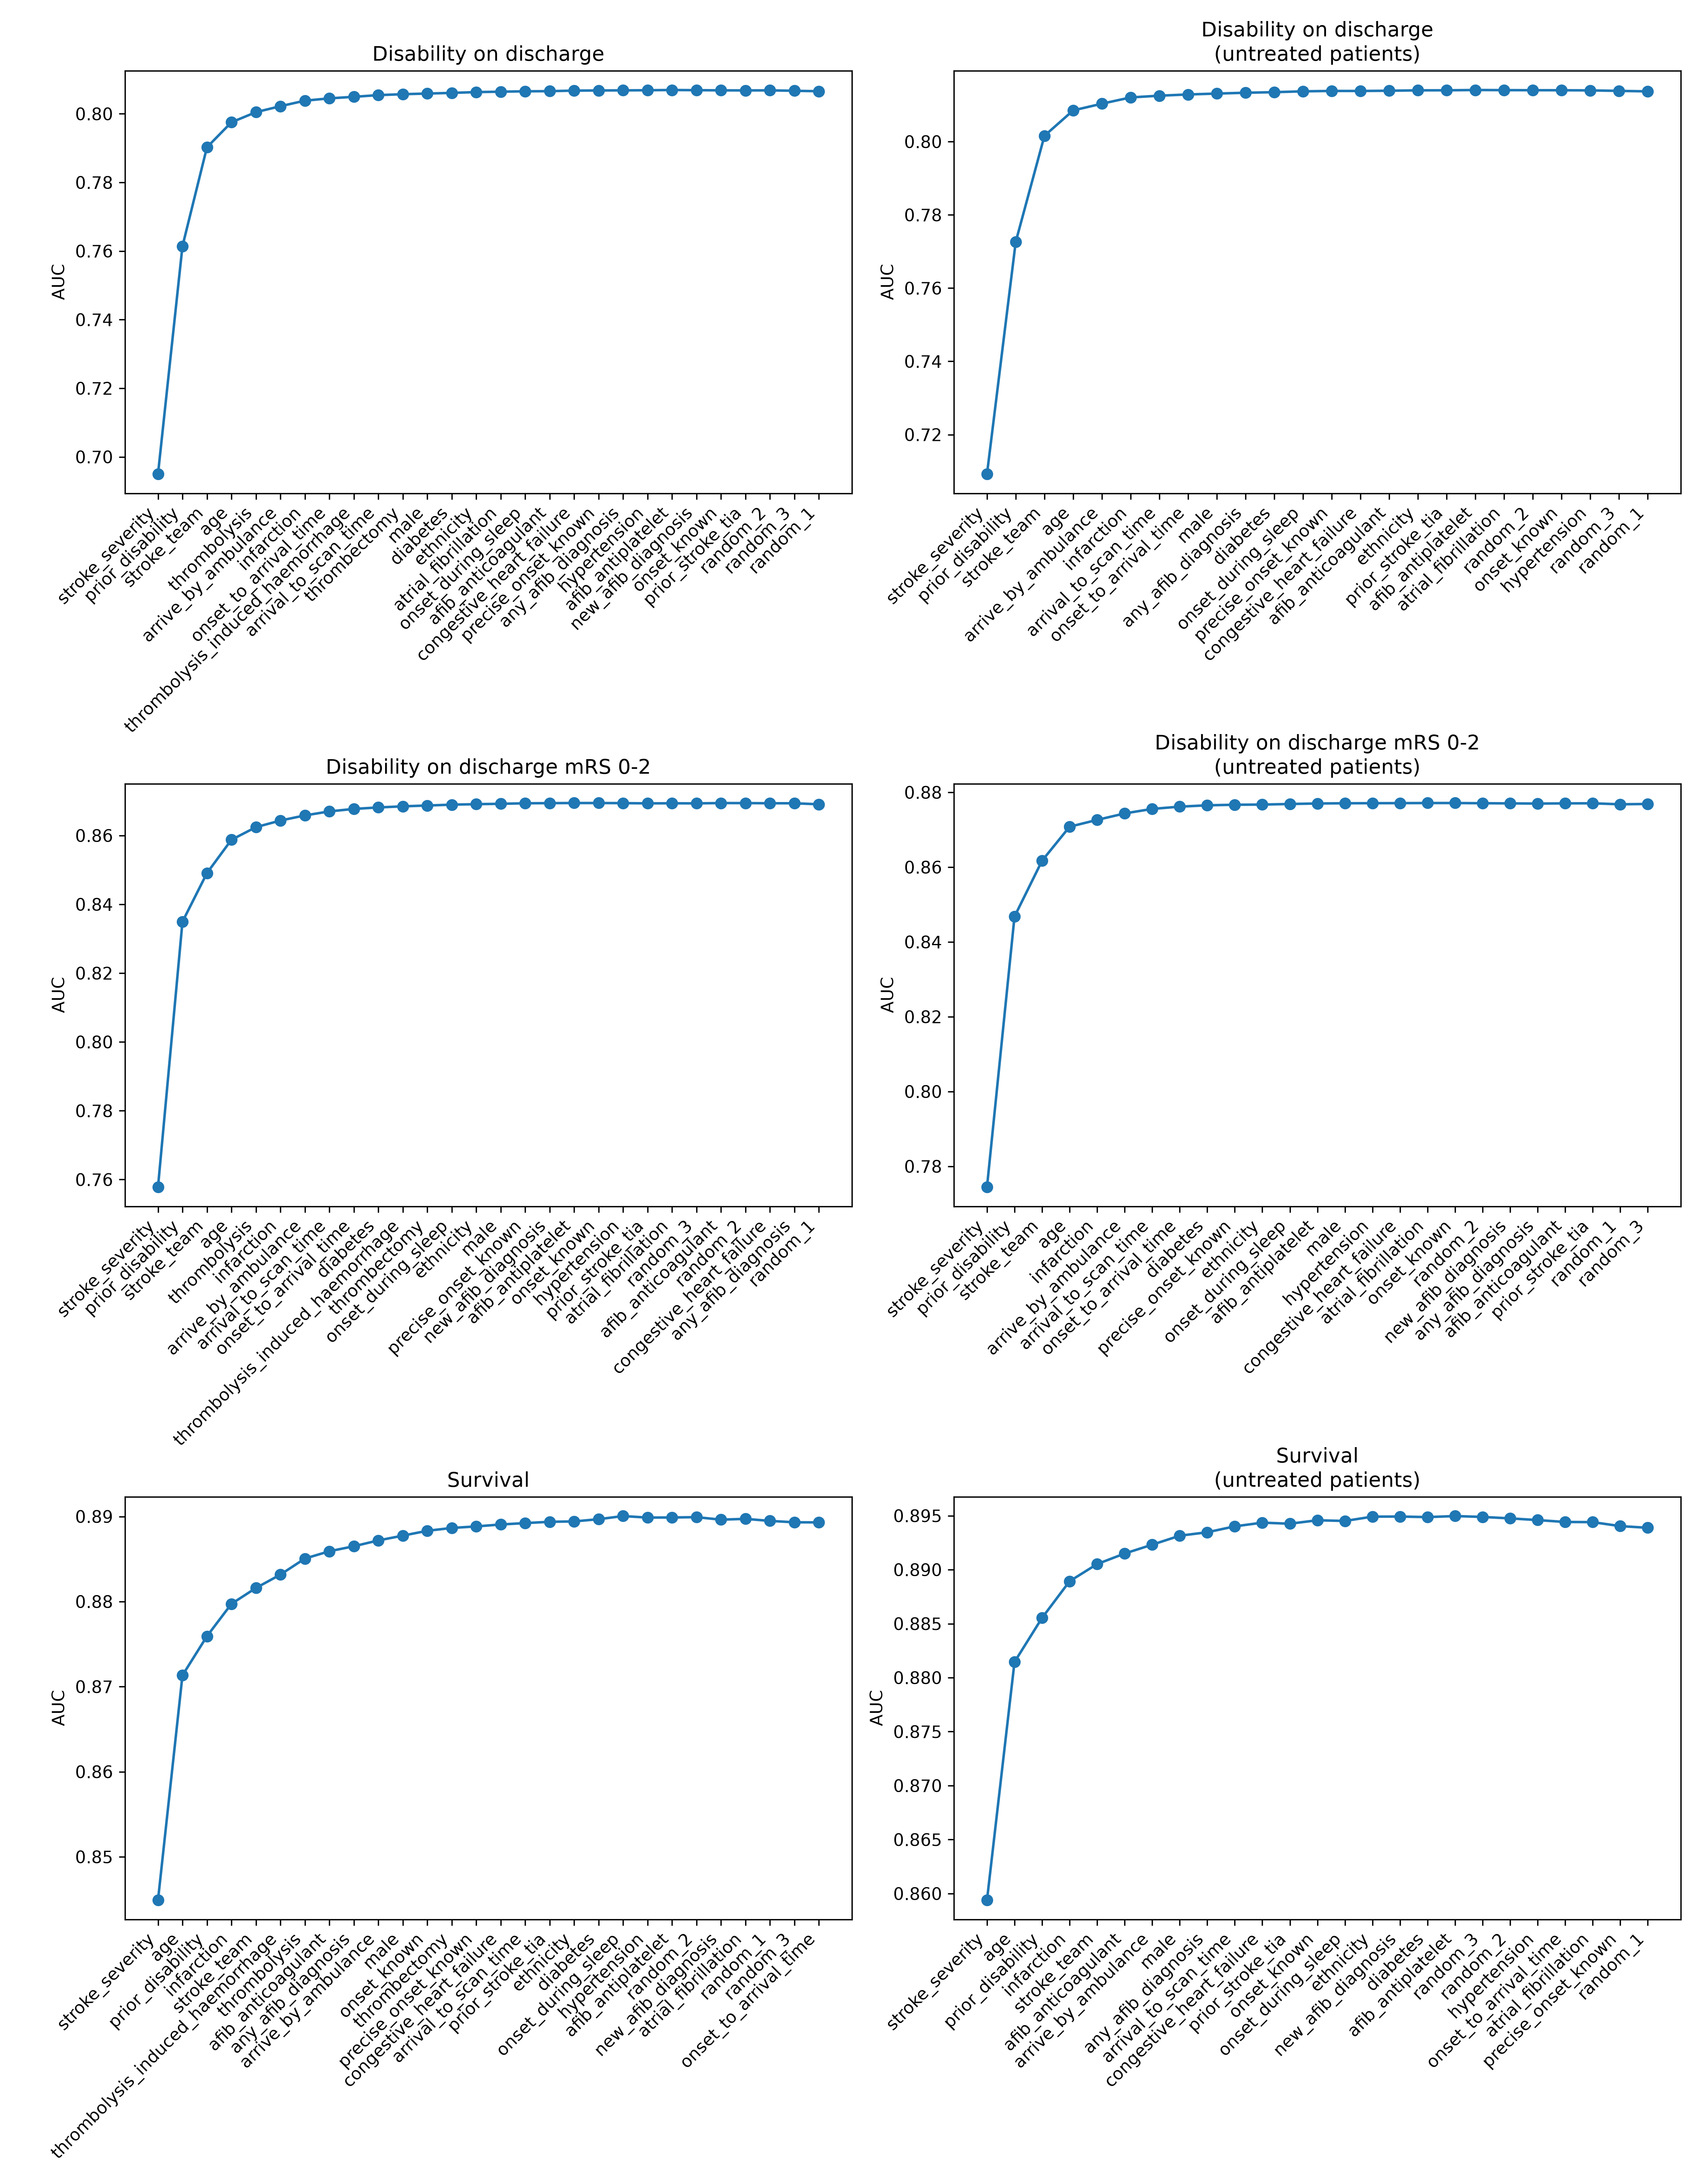
\includegraphics[width=0.98\linewidth]{images/feature_selection/feature_selection_1.png}
    \caption{Feature selection for XGBoost model. Features were selected based on Sequential Forward Selection (SFS) utilizing a greedy search algorithm. Results are shown for mRS disability at discharge for all patients, or those untreated with thrombolysis or thrombectomy (top row), disability at discharge being mRS 0-2 for all patients, or those untreated with thrombolysis or thrombectomy (middle row), and for survival until discharge (for all patients, or those untreated with thrombolysis or thrombectomy (bottom row).}
    \label{fig:feature_selection_1}
\end{figure}

\begin{figure}
    \centering
    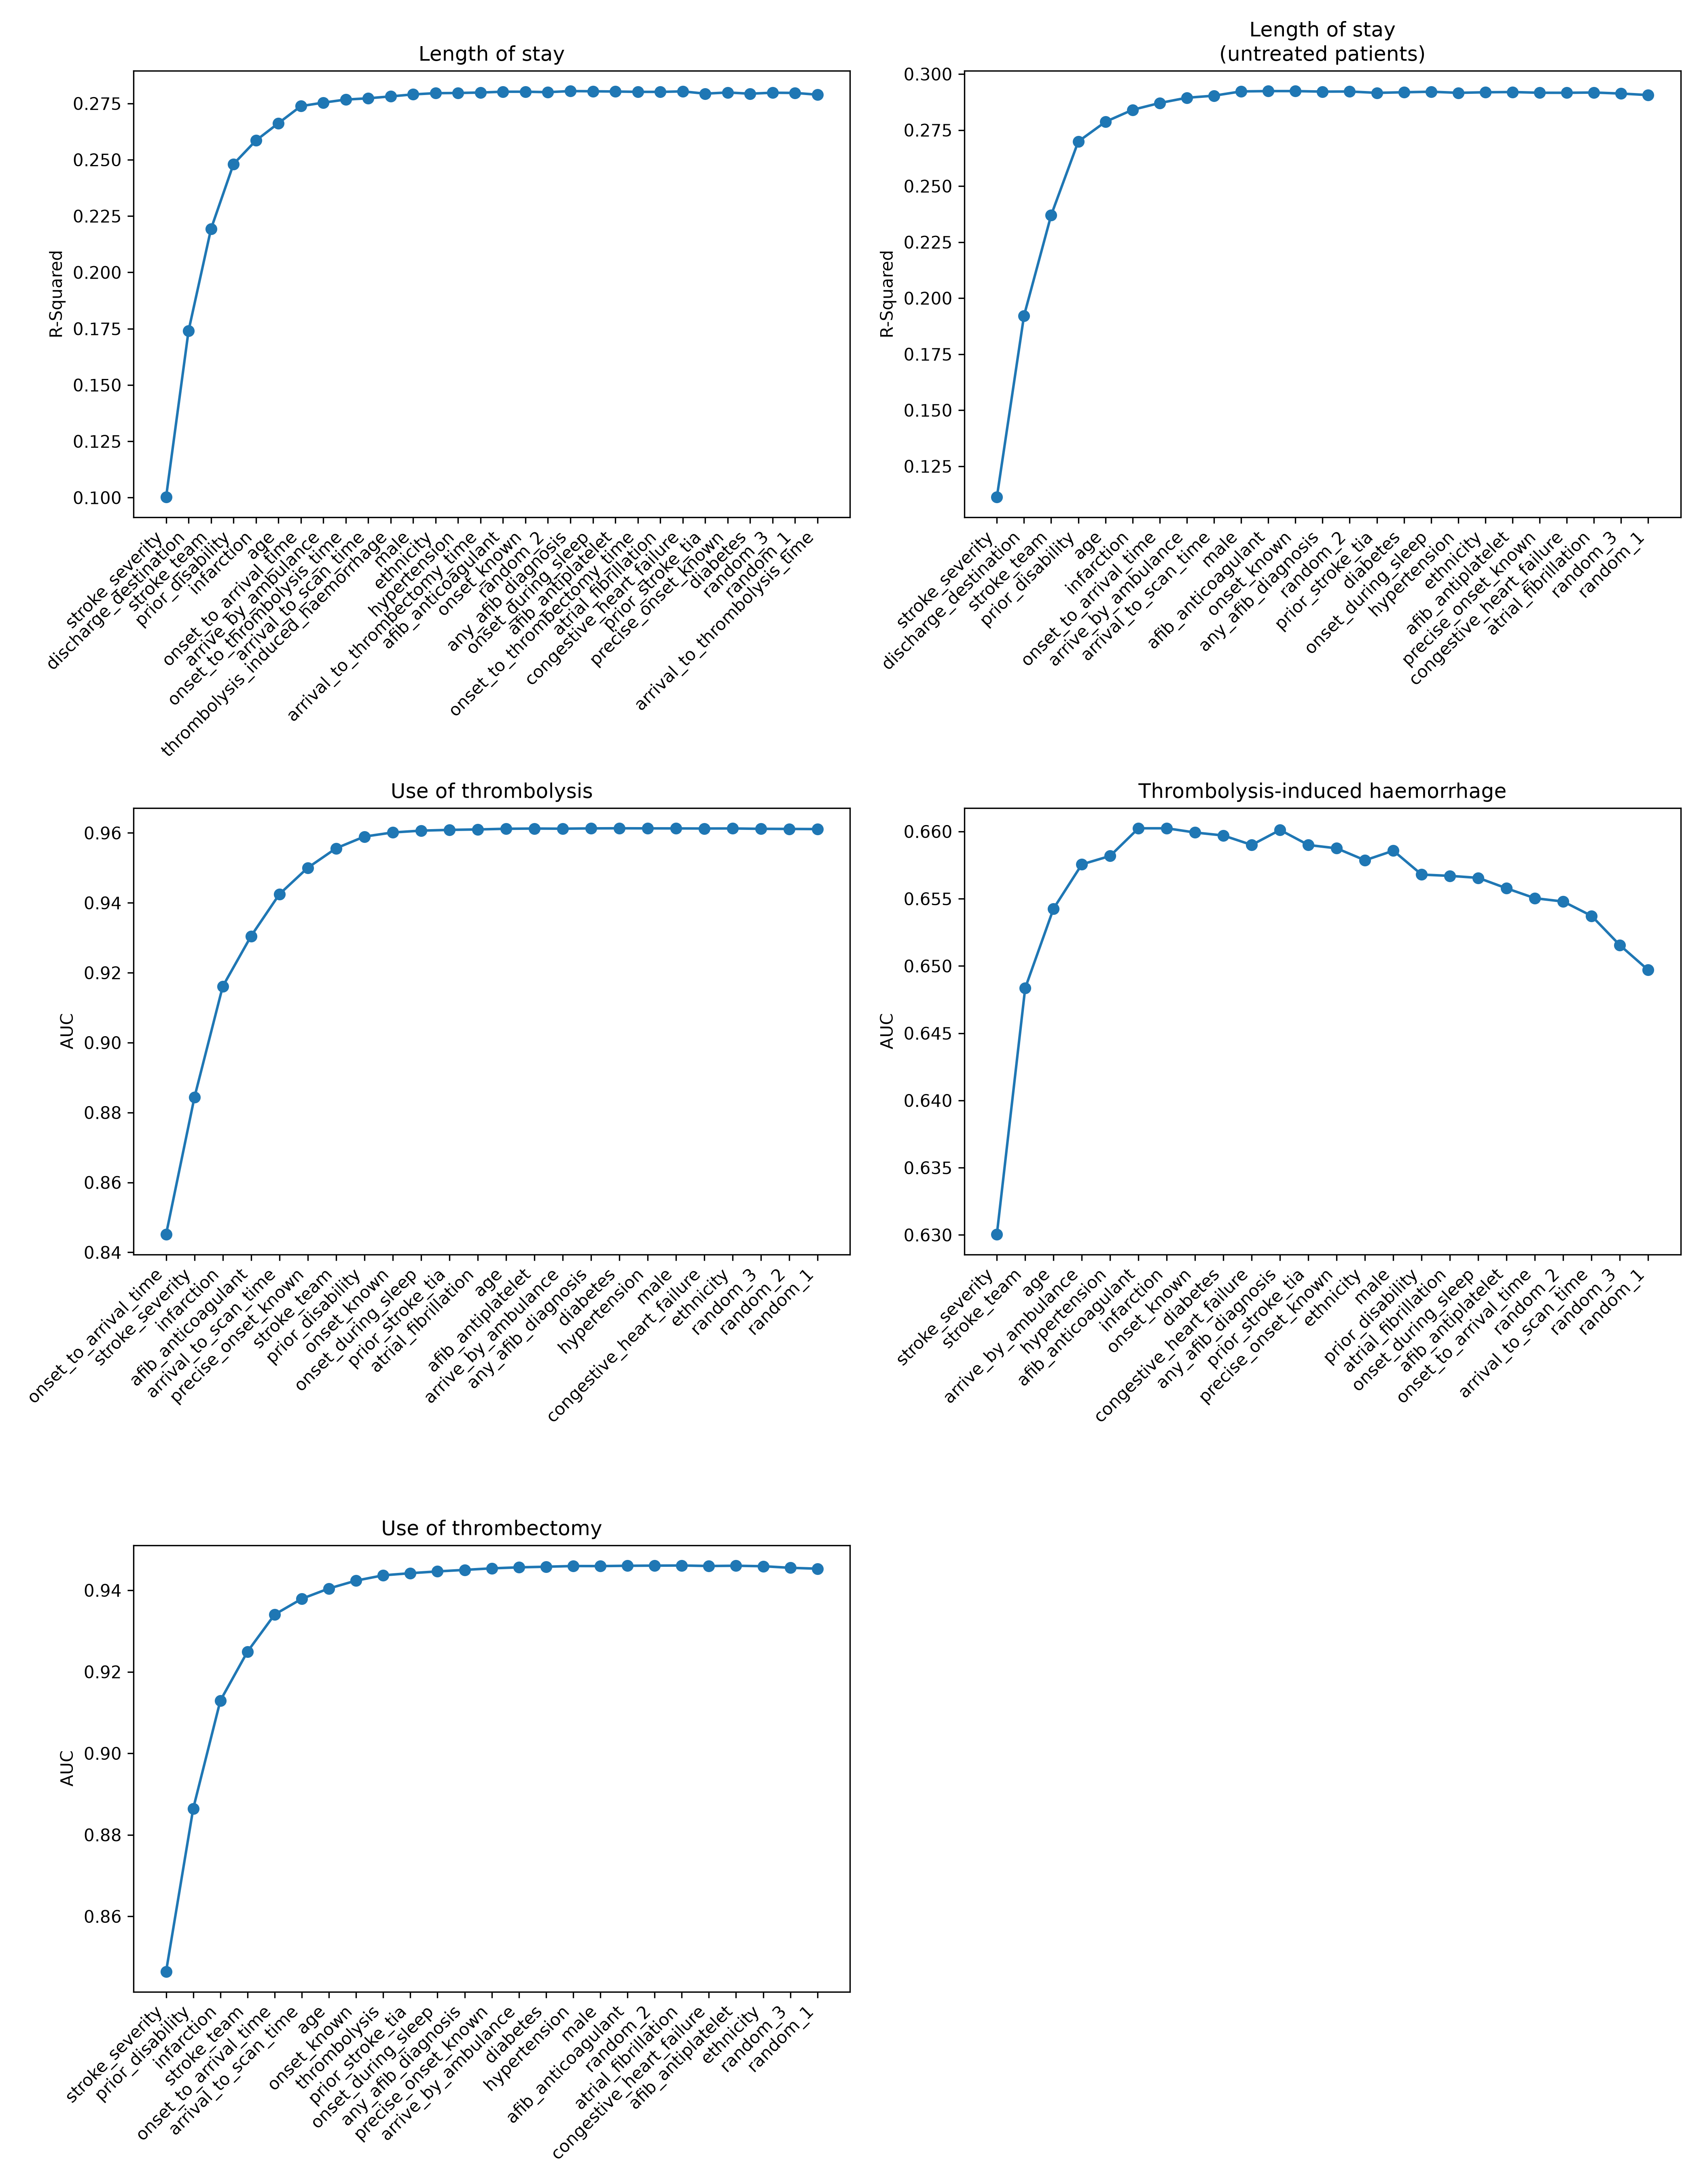
\includegraphics[width=0.98\linewidth]{images/feature_selection/feature_selection_2.png}
    \caption{Feature selection for XGBoost model. Features were selected based on Sequential Forward Selection (SFS) utilizing a greedy search algorithm. Results are shown for length of stay for all patients, or those untreated with thrombolysis or thrombectomy (top row), use of thrombolysis in all patients (middle row, left), thrombolysis-induced haemorrhage in patients receiving thrombolysis (middle row, right), and use of thrombectomy in all patients (bottom row).}
    \label{fig:feature_selection_2}
\end{figure}

% ====================================================================================

\newpage

\section{SHAP analysis}

Figures \ref{fig:shap_mrs0-2_all} to \ref{fig:shap_thrombectomy_all} show SHAP analysis for the different models. SHAP values quantify how each feature, given its specific value for an individual patient, contributed to that patient's model prediction. Each prediction is composed of two parts: a base value, common to all predictions from that model, and the sum of the SHAP values for every feature in that individual's case. Because the model allows for interactions between features, two patients with identical values for a given feature may still receive different SHAP values for that feature, depending on their other characteristics.

The units of the SHAP values depend on the type of model output. For binary outcomes (survival, discharge mRS 0-2, use of thrombolysis or thrombectomy, and thrombolysis-induced haemorrhage), SHAP values are expressed in log-odds; summing them with the base value yields the final log-odds prediction. For the continuous regression outcome (length of stay), SHAP values are expressed in the same units as the outcome itself (days).

In each figure, the top plot is a SHAP \textit{bee-swarm} plot. Feature values are colour-coded from blue (low) to red (high); for stroke severity, for example, blue points indicate low severity and red points indicate high severity. The position on the x-axis shows the SHAP value for each point, with points further to the left indicating that the feature is pushing the model's prediction lower (though this effect may be offset by other features, since SHAP values are additive). Points further to the right indicate the opposite: the feature is pushing the prediction higher. Features are ordered top-to-bottom by their overall importance - specifically, by the mean absolute SHAP value across all instances in the dataset, with the most influential feature at the top and the least influential at the bottom.

Below the top plot in each figure are two further plots showing the SHAP values for the two categorical features, ethnicity and stroke team. Because these features are categorical rather than continuous, they cannot be colour-coded by value in the same way as the bee-swarm plot above; instead, each category is shown separately. For each of the five ethnicity categories (Asian, Black, Mixed, Other/Not Known, White), the SHAP values for that feature—which will depend on interactions with other features—are shown as a violin plot combined with a box plot. The violin plot shows the full distribution and density of SHAP values within each category, while the overlaid box plot summarises this distribution using the median, interquartile range, and outliers, allowing comparison of both central tendency and spread across ethnicity or stroke team categories. SHAP values for stroke teams are shown as a bar chart, with one bar per stroke team representing that team's average SHAP value across all its patients. Bars are ordered from highest to lowest SHAP value, so that teams associated with the largest positive contribution to the model's prediction appear at one end, and those with the largest negative contribution appear at the other.

Though SHAP adds explainability to the model, care should be taken remembering that SHAP values show the influence of a feature value to the final prediction, but that this relationship is not necessarily causal (just as nicotine-stained fingernails may indicate high risk of lung cancer, but the stained nails do not cause the lung cancer). These models and plots are exploratory work, investigating which features may need to be included in later causal models.

Some observations may be made:

\textbf{Prediction of favourable outcome (mRS 0-2) at discharge} (figure \ref{fig:shap_mrs0-2_all}): Lower disability outcomes were especially associated with lower stroke severity, lower prior disability, and lower age. Ischaemic stroke patients had a lower chance of favourable outcomes, compared to haemorrhagic stroke (if all other feature values were similar). The stroke team attended also significantly affected the odds of being discharged mRS 0-2. Black and Asian patients had somewhat lower odds of being discharged mRS 0-2. Lower time to thrombolysis or thrombectomy improved the odds of being discharged mRS 0-2, but longer times to treatment worsened those odds compared to untreated patients. Figure \ref{fig:shap_mrs0-2_no_treatment} repeated the modelling, but for patients not treated with thrombolysis or thrombectomy, confirming that stroke severity, age, prior disability, stroke team and stroke type were the most important features affecting odds of being discharged mRS 0-2, independent of treatment.

\textbf{Prediction of survival until discharge} (figure \ref{fig:shap_survival_all}): Survival was especially associated with lower stroke severity, lower age, and lower prior disability. The stroke team attended also significantly affected the odds of survival. Ischaemic stroke patients had a lower chance of survival, compared to haemorrhagic stroke (if all other feature values were similar). Black, Asian, and Mixed ethnicity patients had \textit{higher} odds of survival compared to white patients (but, as we previously said, with lower odds of being discharged disability-free). Figure \ref{fig:shap_survival_no_treatment} repeated the modelling, but for patients not treated with thrombolysis or thrombectomy, confirming that stroke severity, age, prior disability, stroke team and stroke type were the most important features affecting odds of survival to discharge, independent of treatment.

\textbf{Prediction of length of stay} (figure \ref{fig:shap_los_all}): Higher stroke severity was associated with longer lengths of stay, though dying in hospital was associated with shorter lengths of stay, as was being discharged to a community or early-supported discharge team. Stroke team attended had a significant effect on prediction of length of stay. Shorter onset-to-arrival times were associated with lower lengths of stay.

\textbf{Use of thrombolysis} (figure \ref{fig:shap_thrombolysis_all}): Key features associated with higher odds of use of thrombolysis were: shorter onset-to-arrival and arrival-to-scan times, infarction stroke, higher stroke severity, no use of atrial fibrillation anticoagulation, and lower prior disability. Odds of receiving thrombolysis were slightly lower in Black and Mixed ethnicity groups. Stroke team attended had a significant association with odds of receiving thrombolysis.

\textbf{Use of thrombectomy} (figure \ref{fig:shap_thrombectomy_all}): Key features associated with higher odds of use of thrombectomy were: higher stroke severity, infarction stroke, shorter onset-to-arrival and arrival-to-scan times, lower prior disability, and lower age. Odds of receiving thrombectomy were  lower in Black, Asian and Mixed ethnicity groups. Stroke team attended had a significant association with odds of receiving thrombectomy.

\textbf{Thrombolysis-induced haemorrhage, in patients receiving thrombolysis} (figure \ref{fig:shap_thrombolysis_haemorrhage}): Though this model had lower predictive scores, SHAP is included here for completeness. Odds of thrombolysis causing haemorrhage were higher with shorter onset-to-arrival times, higher stroke severity, lower arrival-to-scan times, and lower pre-stroke disability. Stroke team attended had a significant association with odds of thrombolysis-induced haemorrhage.

%%%%%%%%%%% Discharge disability 0-2 %%%%%%%%%%%%%%%

%% All patients

\begin{figure}[htbp]
    \centering
    
    % Top image (Full width)
    \begin{subfigure}{0.50\textwidth}
        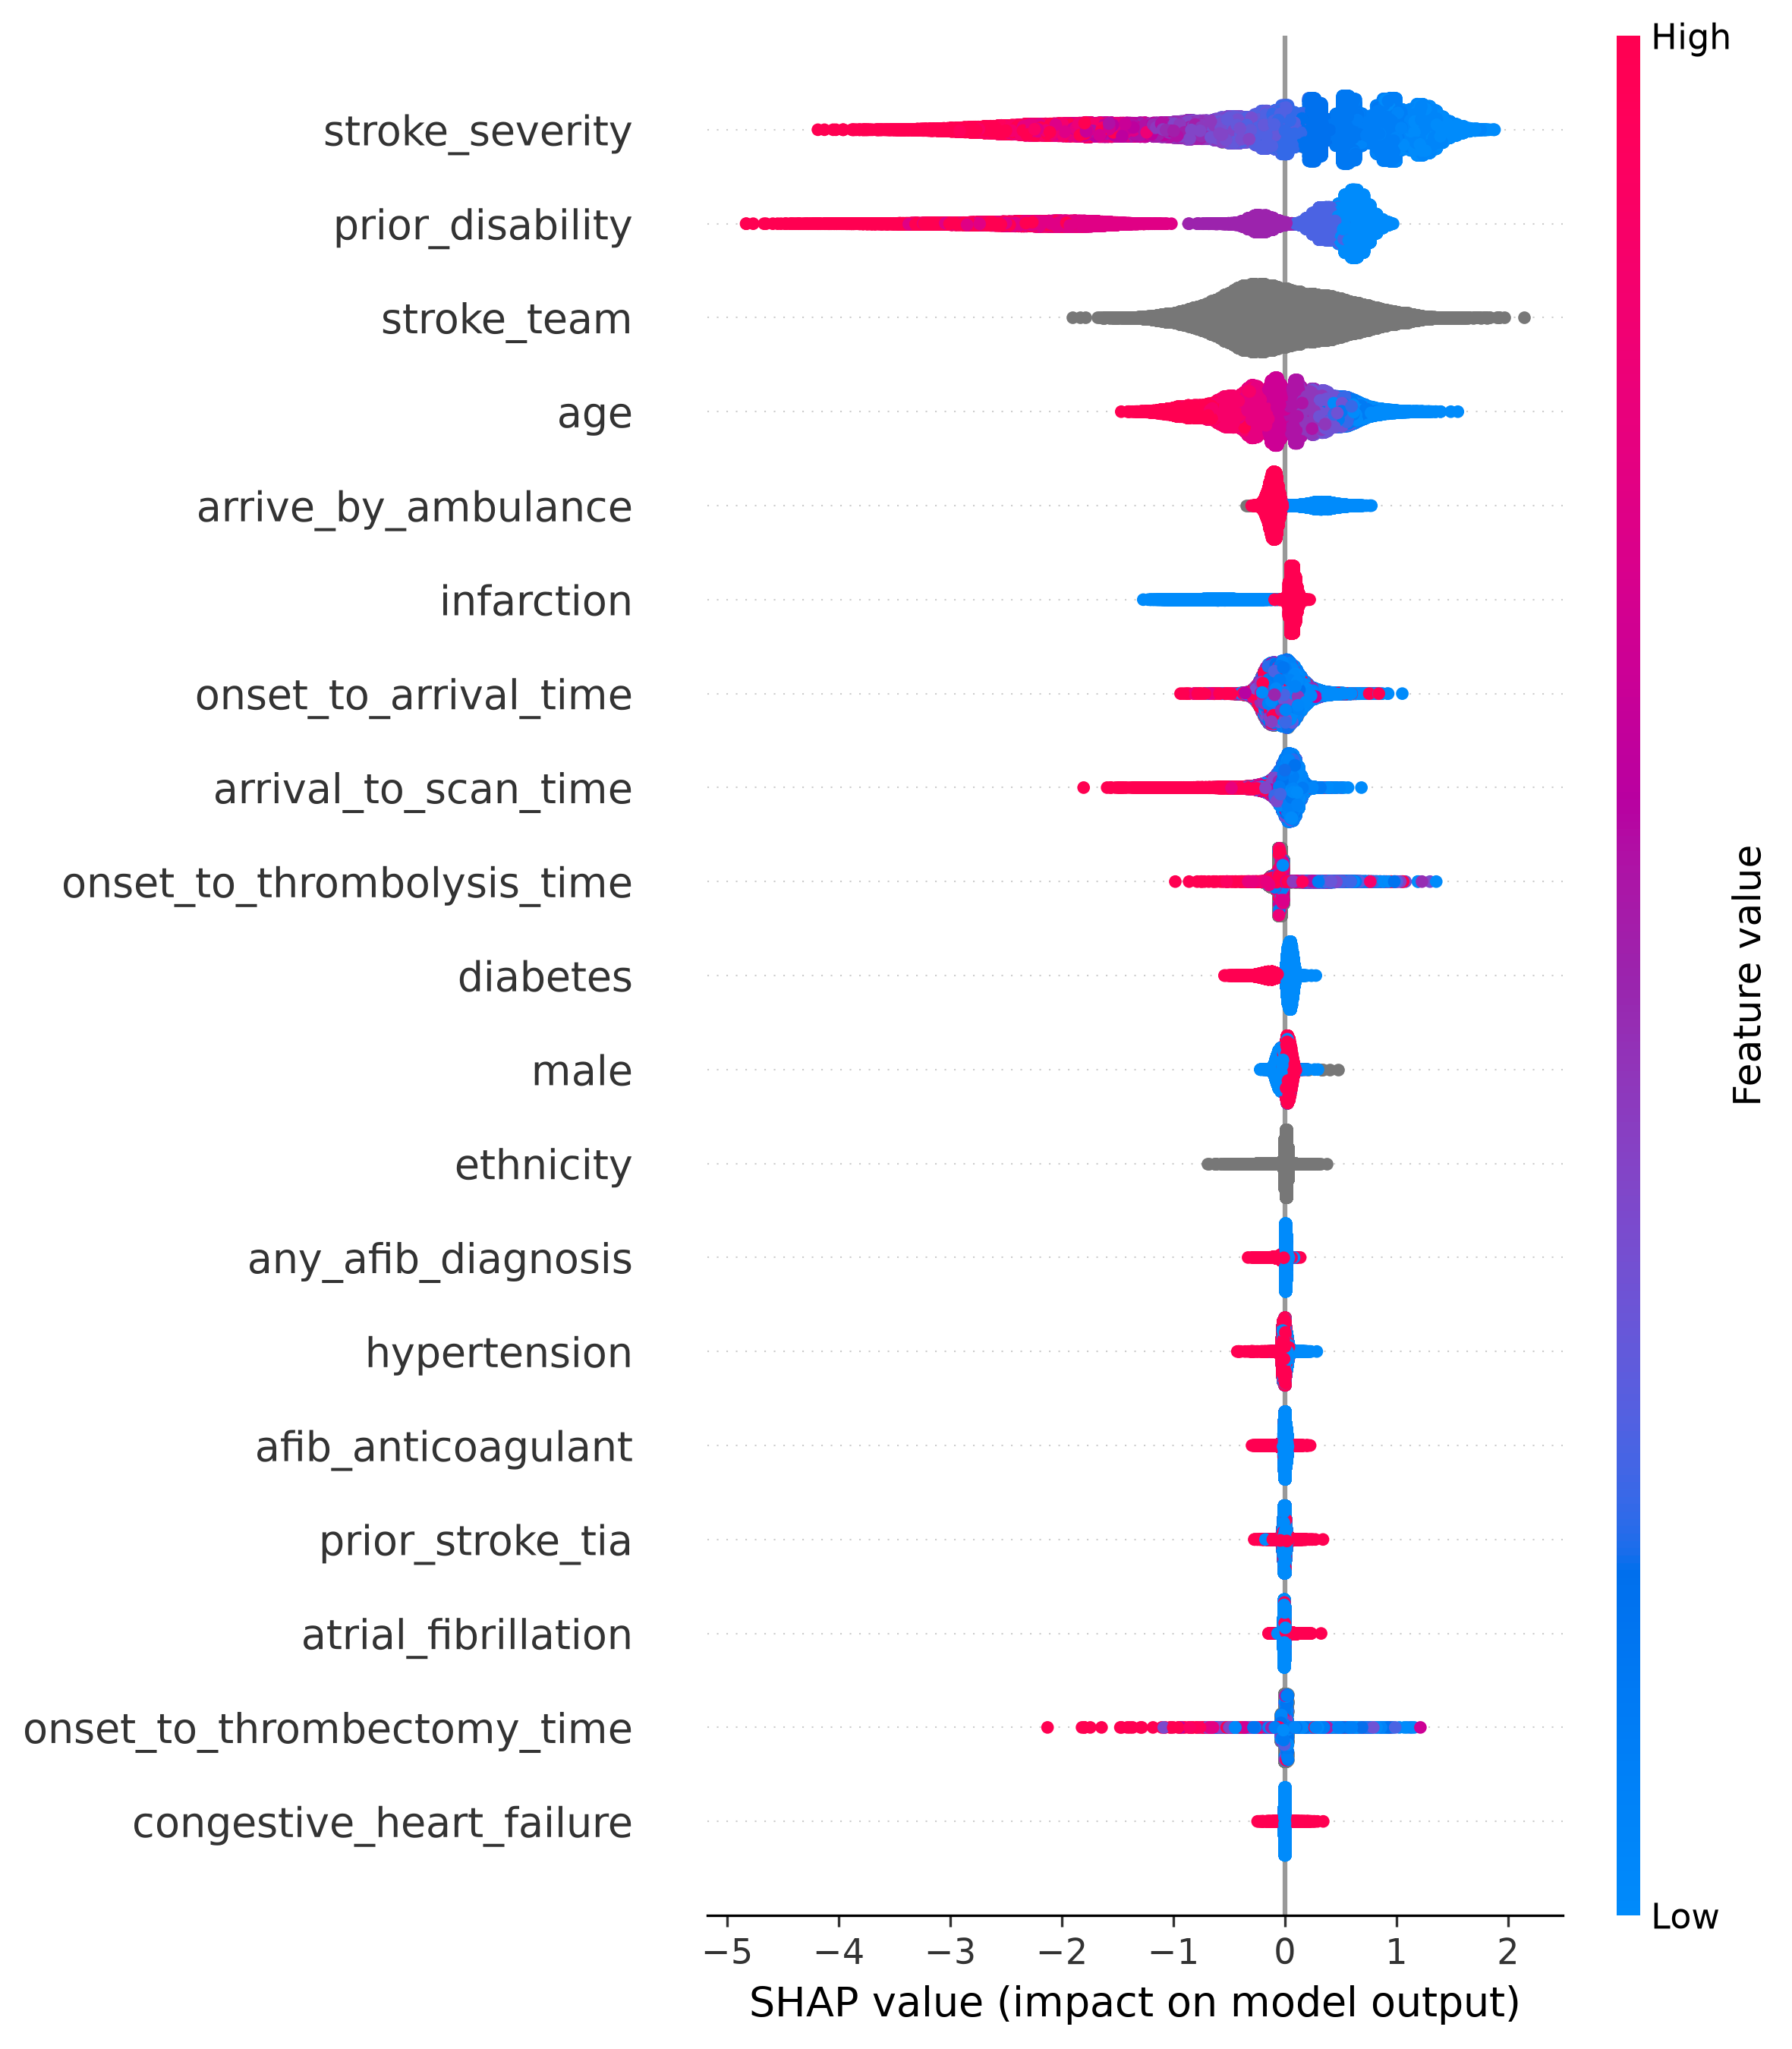
\includegraphics[width=\linewidth]{images/shap/shap_all_patients_mrs_less_than_3.png}
        %\caption{}
    \end{subfigure}

    \vspace{0.5cm} % Optional vertical space between rows

    % Bottom left image (~45% width)
    \begin{subfigure}{0.407\textwidth}
        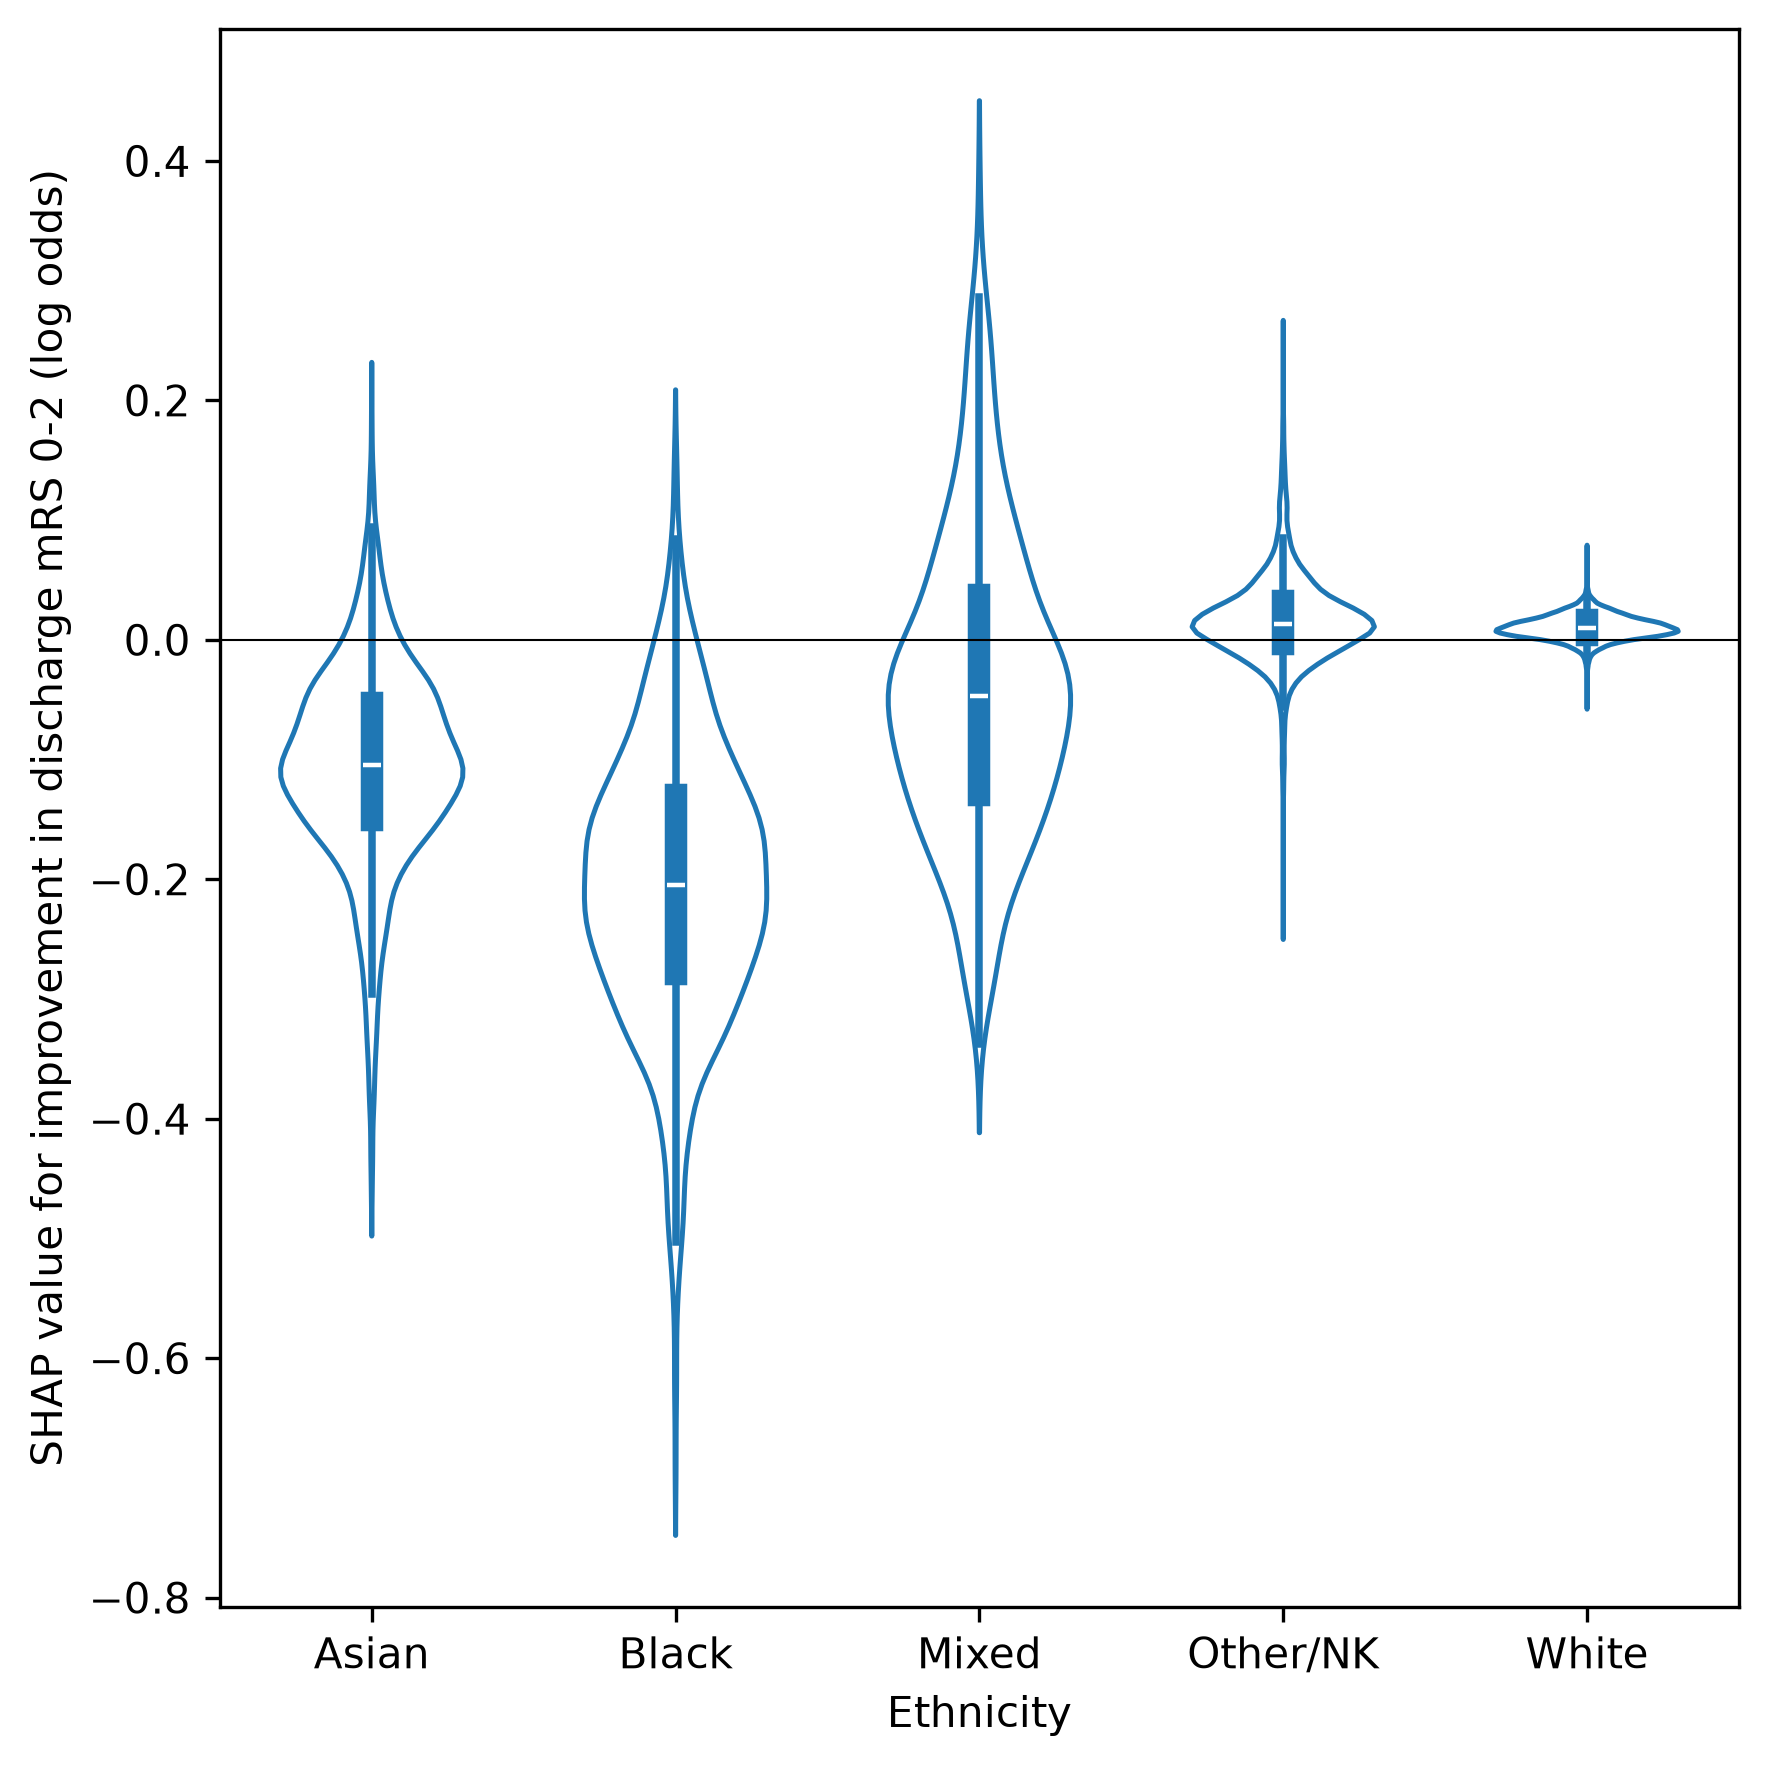
\includegraphics[width=\linewidth]{images/shap/shap_all_patients_mrs_less_than_3_ethnicity.png}
        %\caption{}
    \end{subfigure}
    \hfill % Adds flexible horizontal spacing
    % Bottom right image (~55% width)
    \begin{subfigure}{0.543\textwidth}
        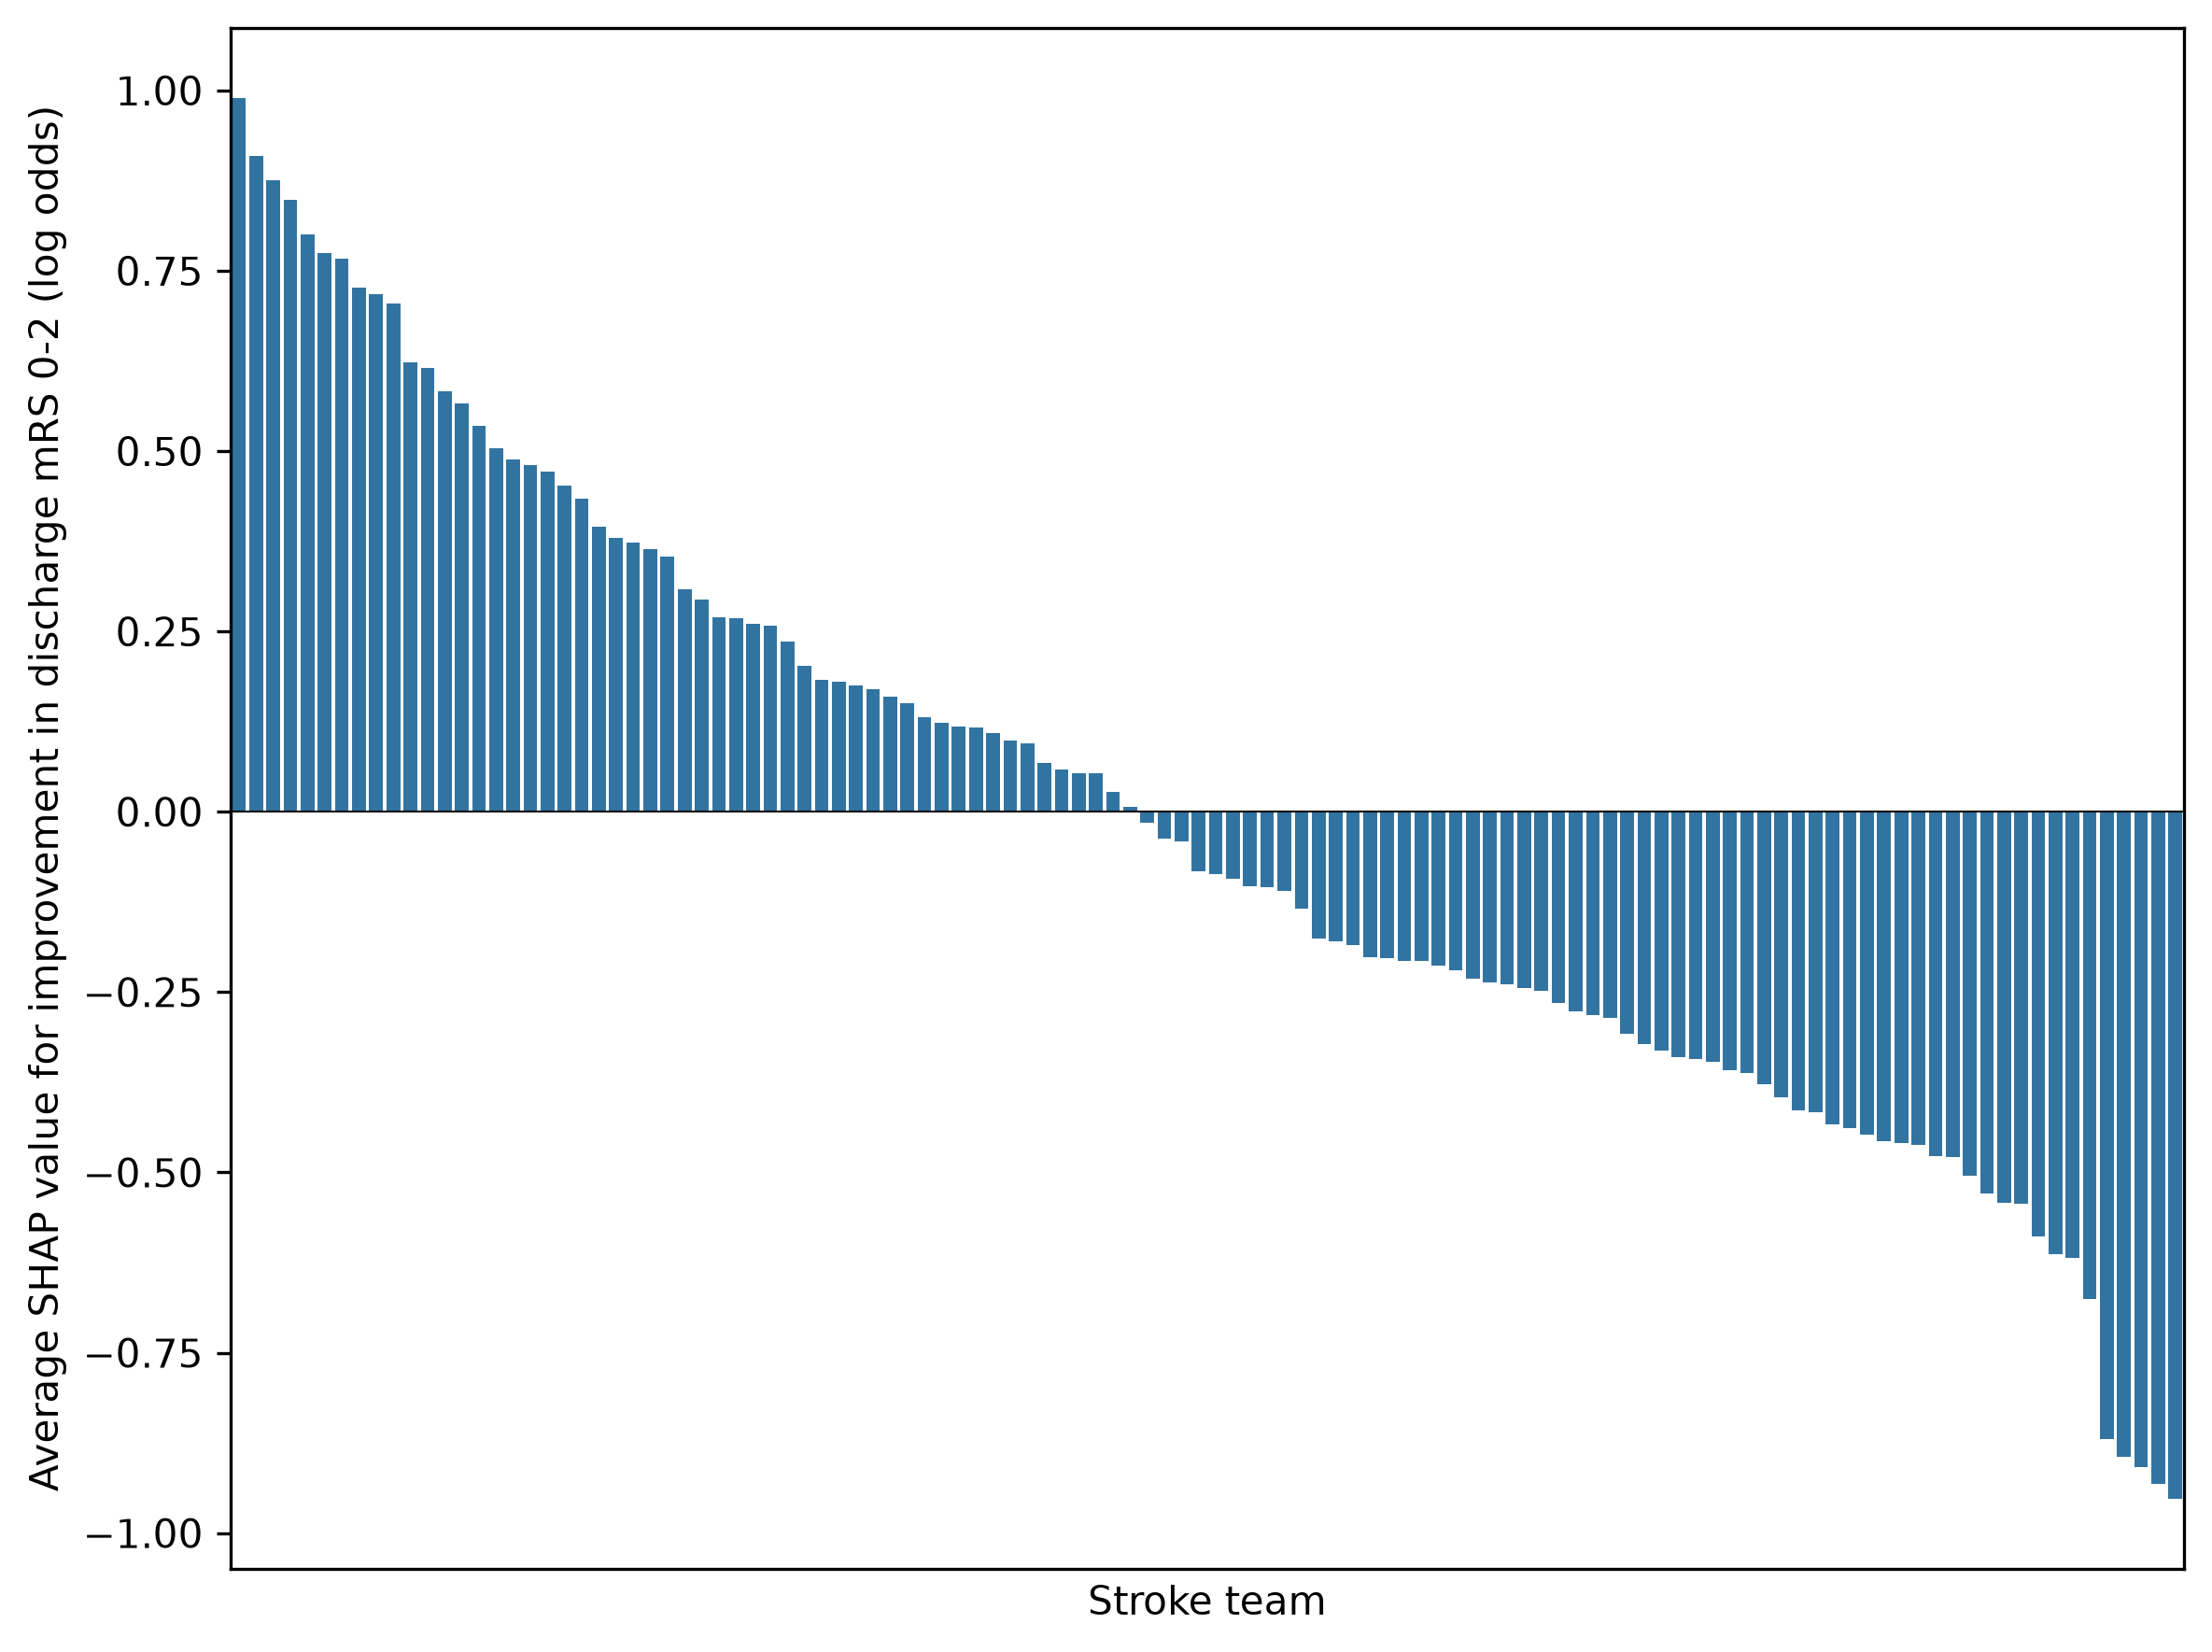
\includegraphics[width=\linewidth]{images/shap/shap_all_patients_mrs_less_than_3_stroke_team.png}
        %\caption{}
    \end{subfigure}

    \caption{SHAP analysis of feature contributions to predicting favourable discharge outcomes (mRS 0-2) in stroke patients. \textit{Top}: A SHAP summary plot detailing the impact of features on the model's log-odds predictions. Each point represents an individual patient instance. The position on the x-axis indicates the SHAP value, where positive values increase the predicted odds of a favourable outcome, and negative values decrease it. For continuous and binary variables, colour represents the original feature value (red indicating high values; blue indicating low values). Categorical variables (\textit{stroke team} and \textit{ethnicity}) are plotted in grey. \textit{Bottom left}: Violin plots illustrating the distribution of SHAP values across distinct ethnic groups. This panel highlights the marginal impact and variance of ethnicity on the model’s prediction for disability outcome. \textit{Bottom Right}: A ranked bar chart displaying the average SHAP value associated with each individual stroke team. This panel visualizes institutional variation, reflecting the contribution of the treating stroke team to the predicted patient outcome after accounting for patient-level clinical characteristics.}
    \label{fig:shap_mrs0-2_all}
\end{figure}

%% Untreated patients

\begin{figure}[htbp]
    \centering
    
    % Top image (Full width)
    \begin{subfigure}{0.50\textwidth}
        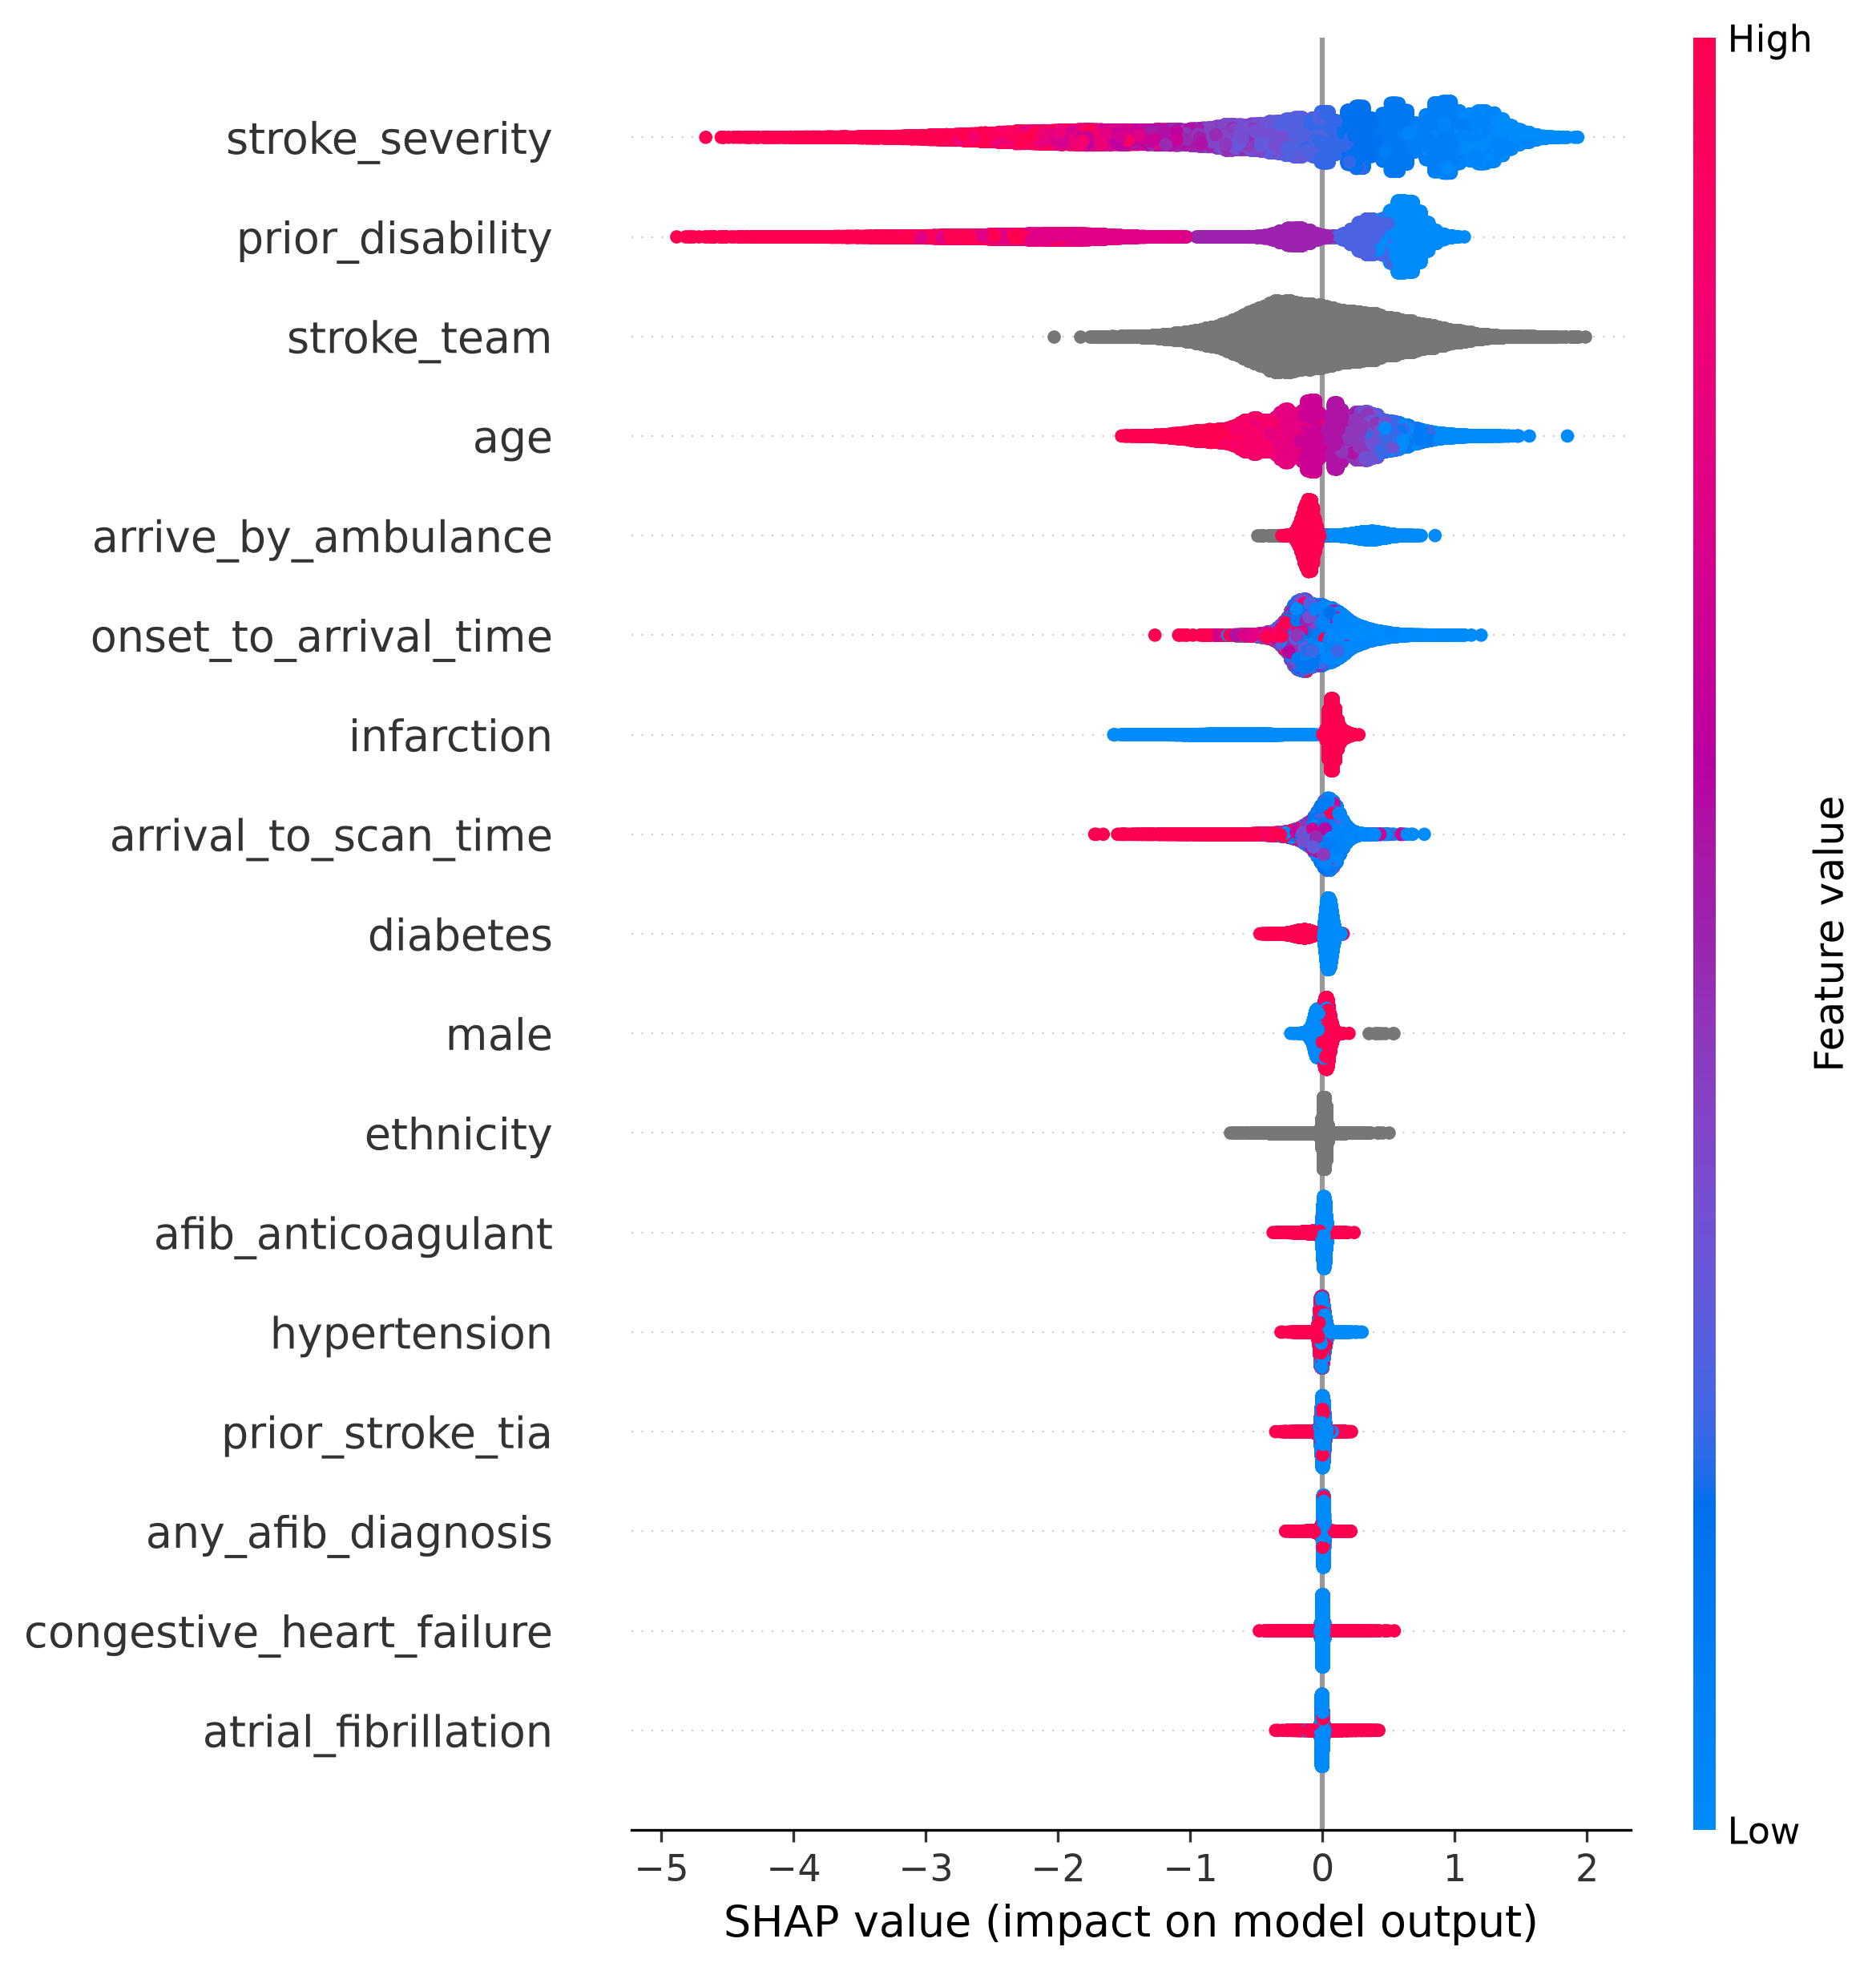
\includegraphics[width=\linewidth]{images/shap/shap_untreated_patients_mrs_less_than_3.png}
        %\caption{}
    \end{subfigure}

    \vspace{0.5cm} % Optional vertical space between rows

    % Bottom left image (~45% width)
    \begin{subfigure}{0.407\textwidth}
        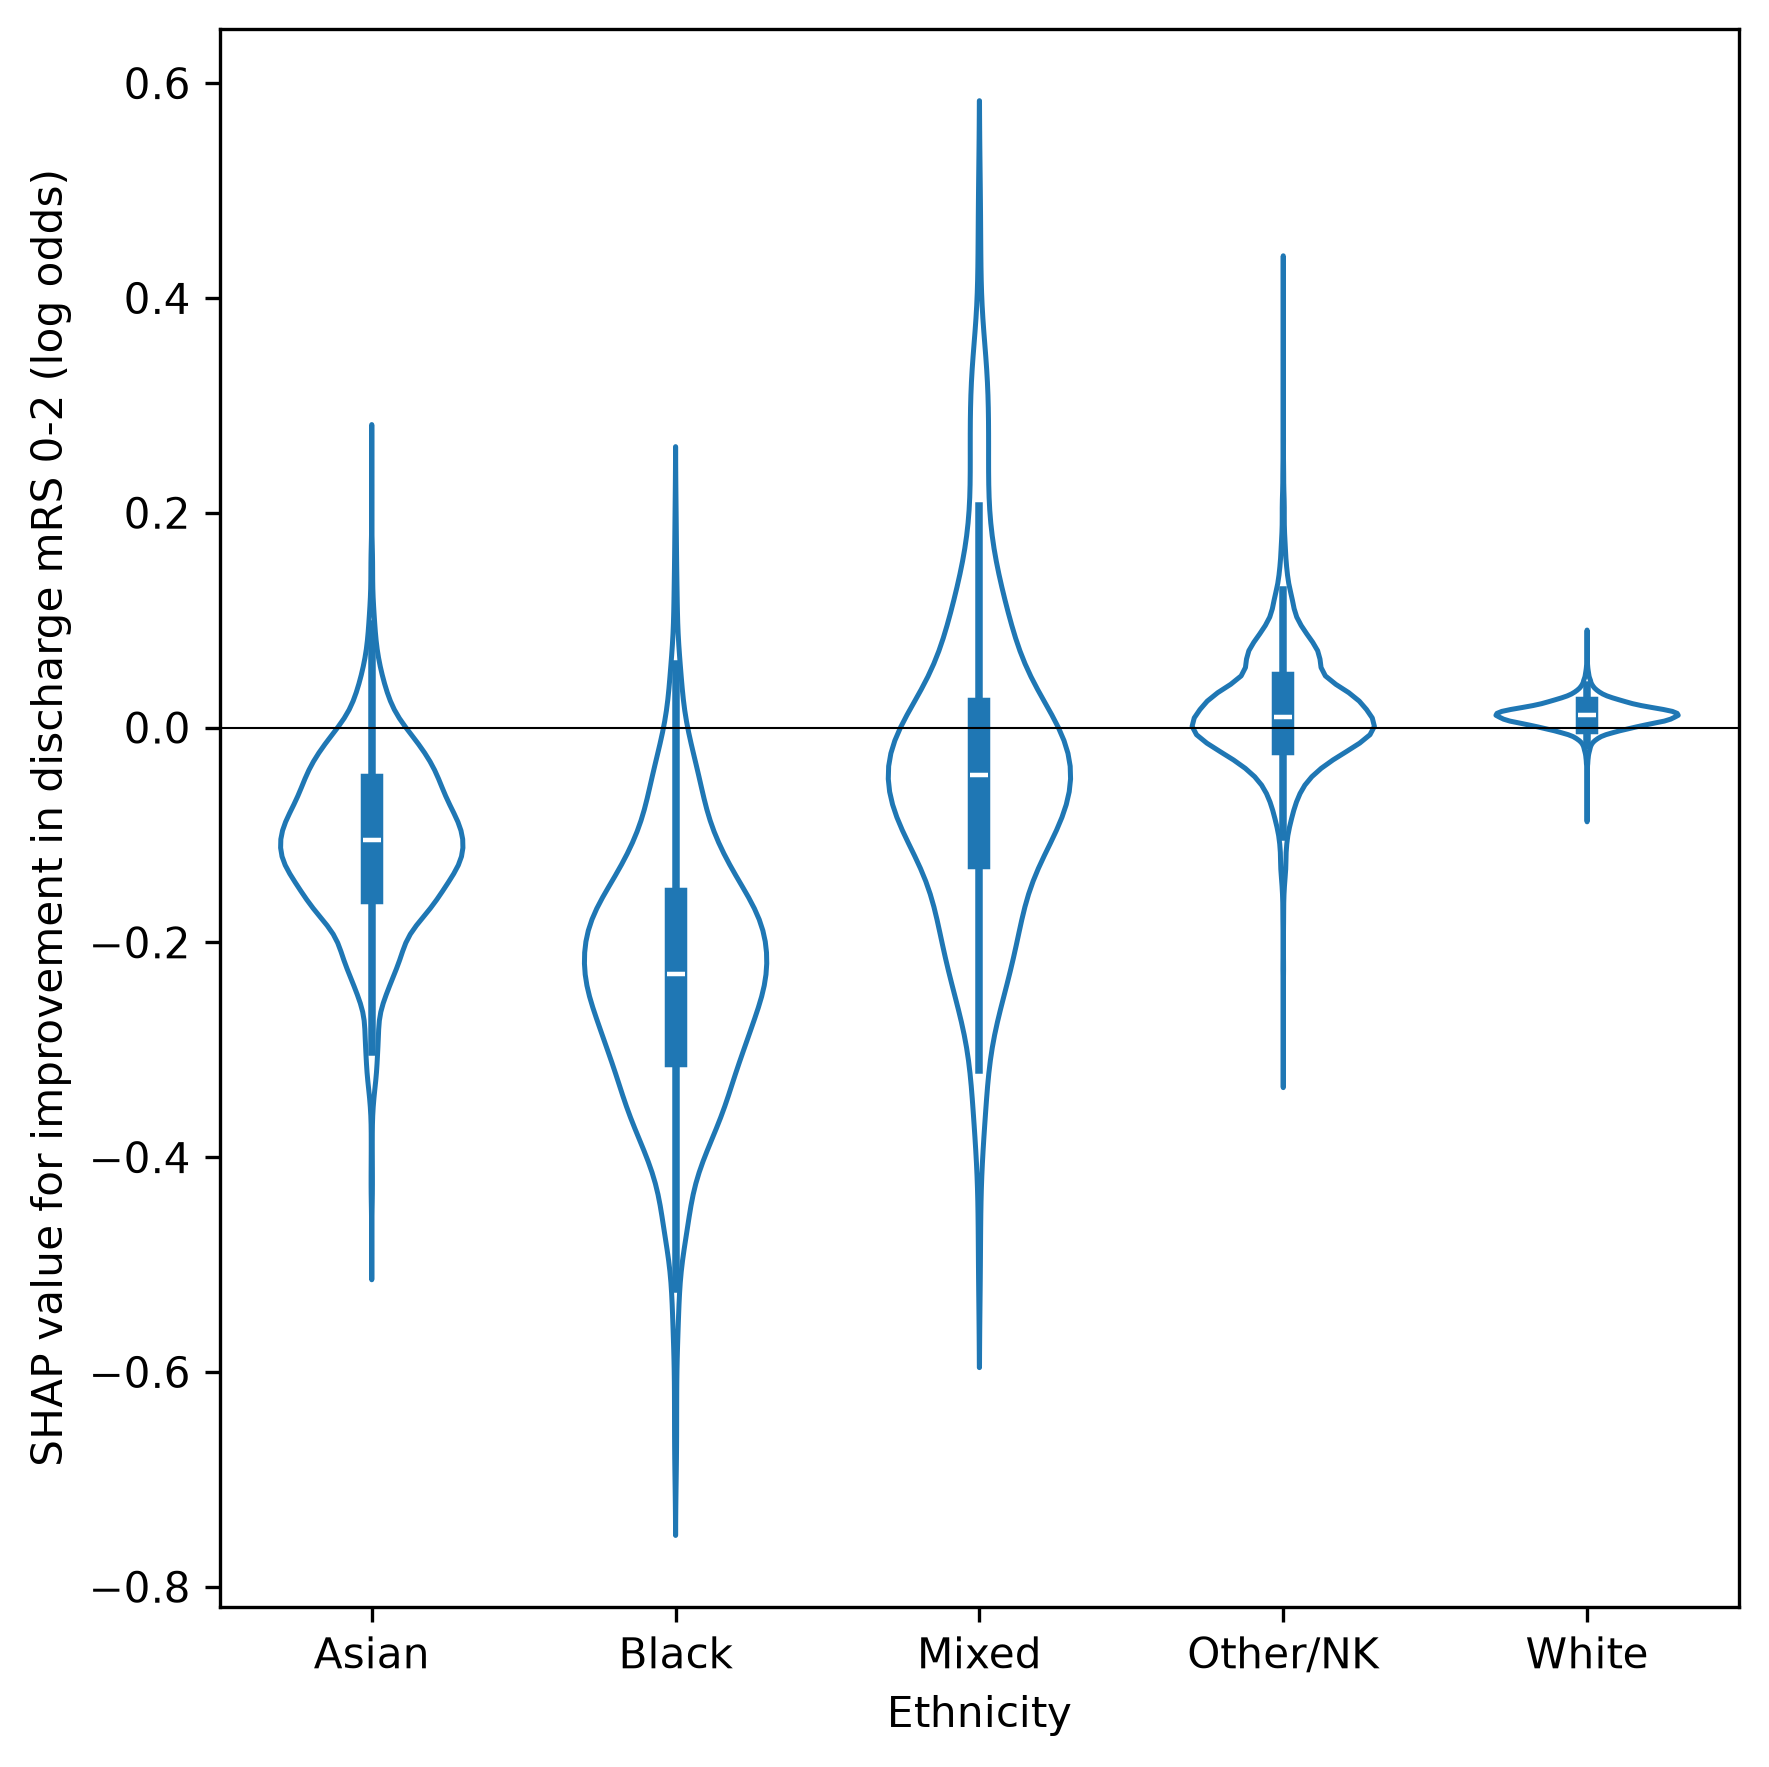
\includegraphics[width=\linewidth]{images/shap/shap_untreated_patients_mrs_less_than_3_ethnicity.png}
        %\caption{}
    \end{subfigure}
    \hfill % Adds flexible horizontal spacing
    % Bottom right image (~55% width)
    \begin{subfigure}{0.543\textwidth}
        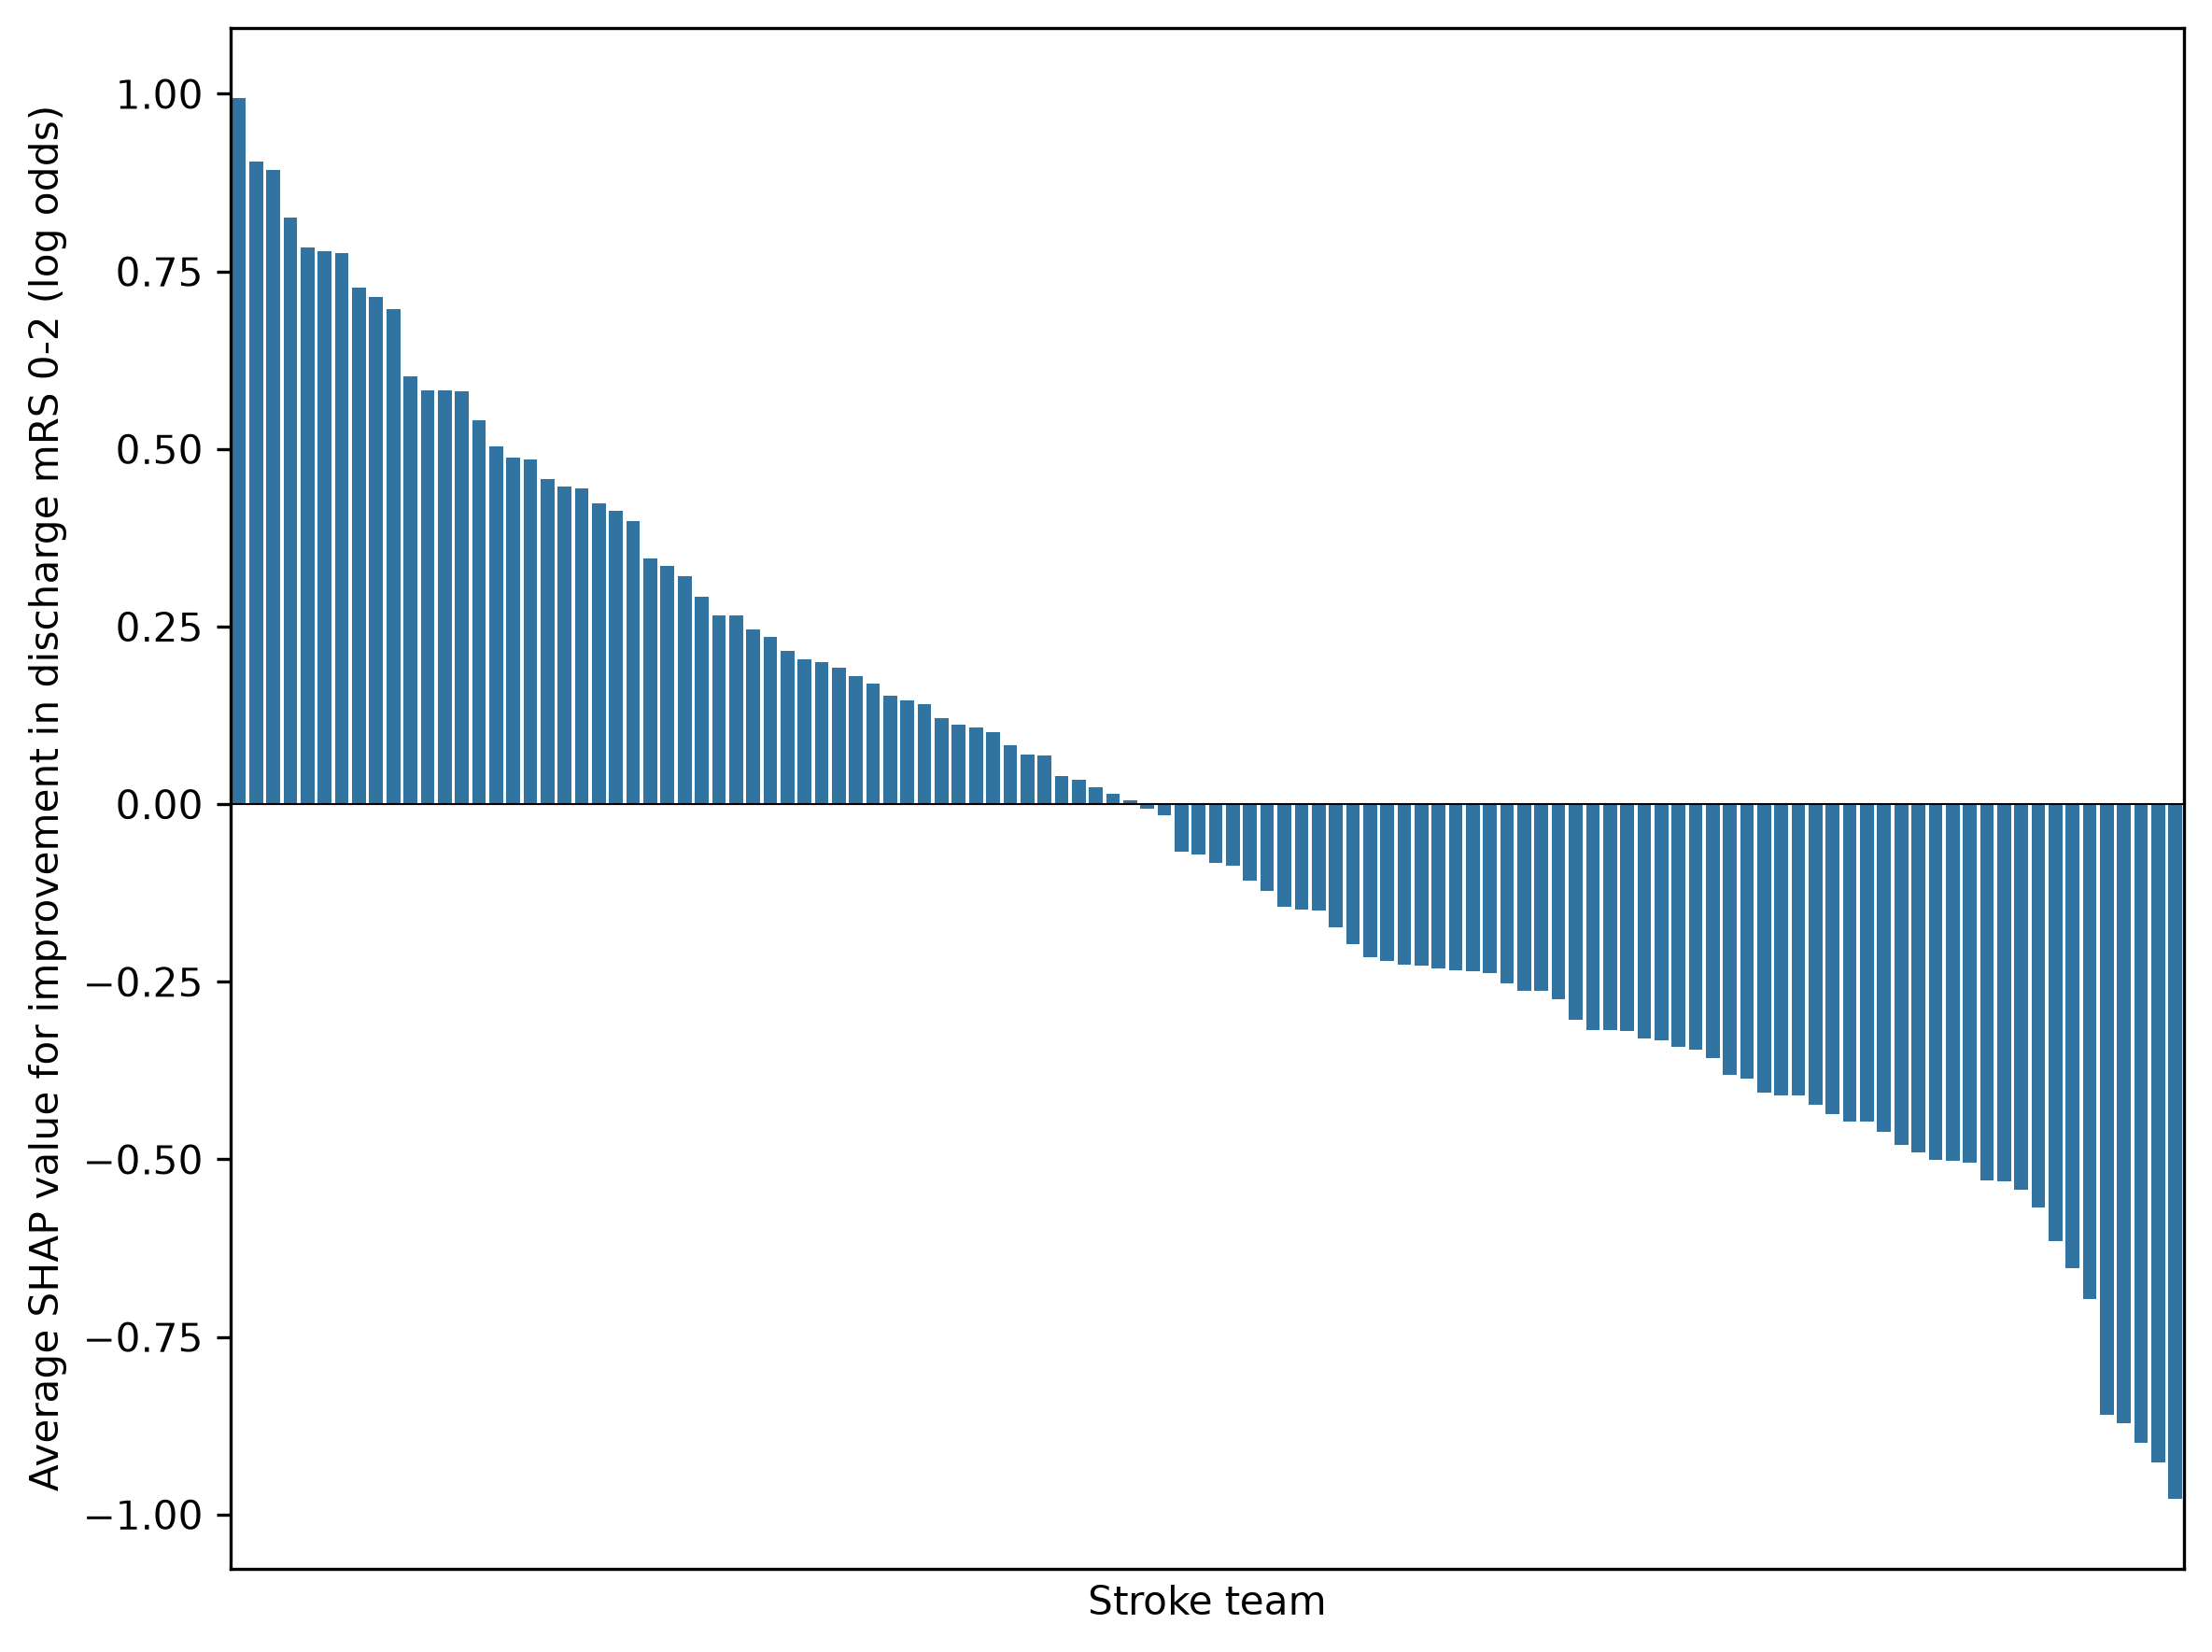
\includegraphics[width=\linewidth]{images/shap/shap_untreated_patients_mrs_less_than_3_stroke_team.png}
        %\caption{}
    \end{subfigure}

    \caption{SHAP analysis of feature contributions to predicting favourable discharge outcomes (mRS 0-2) in stroke patients who did not receive thrombolysis or thrombectomy. \textit{Top}: A SHAP summary plot detailing the impact of features on the model's log-odds predictions. Each point represents an individual patient instance. The position on the x-axis indicates the SHAP value, where positive values increase the predicted odds of a favourable outcome, and negative values decrease it. For continuous and binary variables, colour represents the original feature value (red indicating high values; blue indicating low values). Categorical variables (\textit{stroke team} and \textit{ethnicity}) are plotted in grey. \textit{Bottom left}: Violin plots illustrating the distribution of SHAP values across distinct ethnic groups. This panel highlights the marginal impact and variance of ethnicity on the model’s prediction for disability outcome. \textit{Bottom Right}: A ranked bar chart displaying the average SHAP value associated with each individual stroke team. This panel visualizes institutional variation, reflecting the contribution of the treating stroke team to the predicted patient outcome after accounting for patient-level clinical characteristics.}
    \label{fig:shap_mrs0-2_no_treatment}
\end{figure}

%%%%%%%%%%% Survival %%%%%%%%%%%%%%%

%% All patients

\begin{figure}[htbp]
    \centering
    
    % Top image (Full width)
    \begin{subfigure}{0.50\textwidth}
        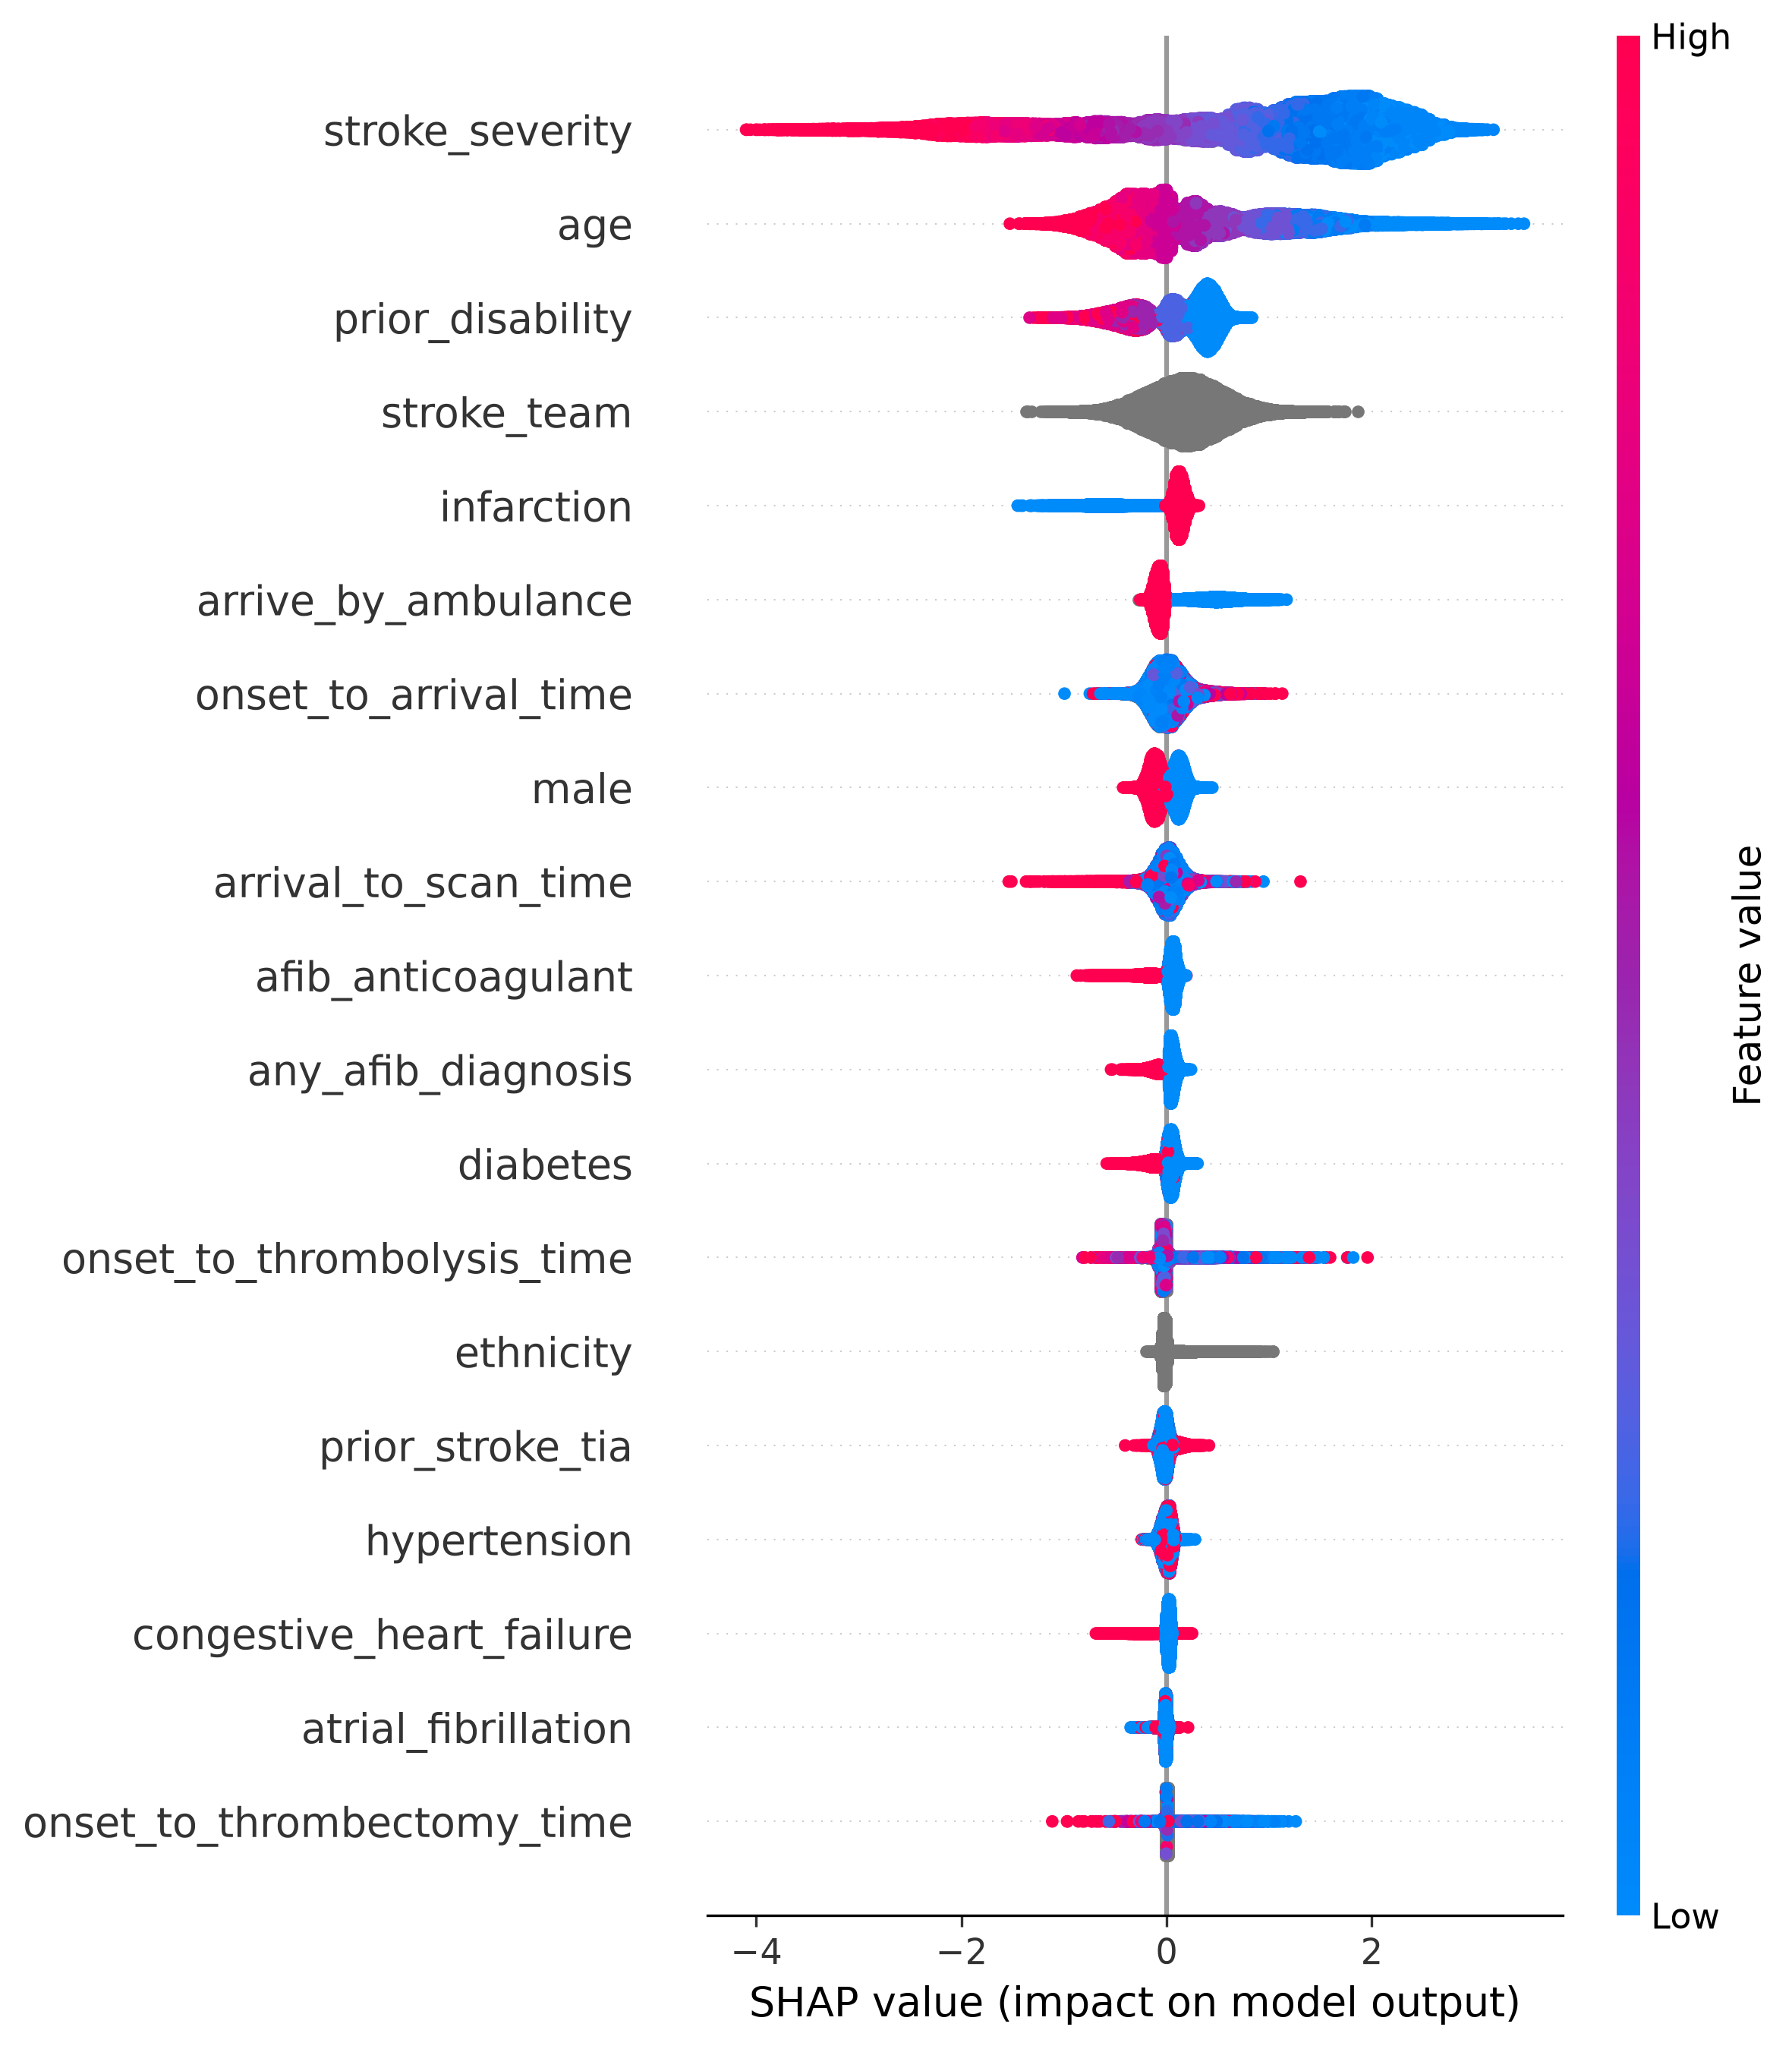
\includegraphics[width=\linewidth]{images/shap/shap_all_patients_survival.png}
        %\caption{}
    \end{subfigure}

    \vspace{0.5cm} % Optional vertical space between rows

    % Bottom left image (~45% width)
    \begin{subfigure}{0.407\textwidth}
        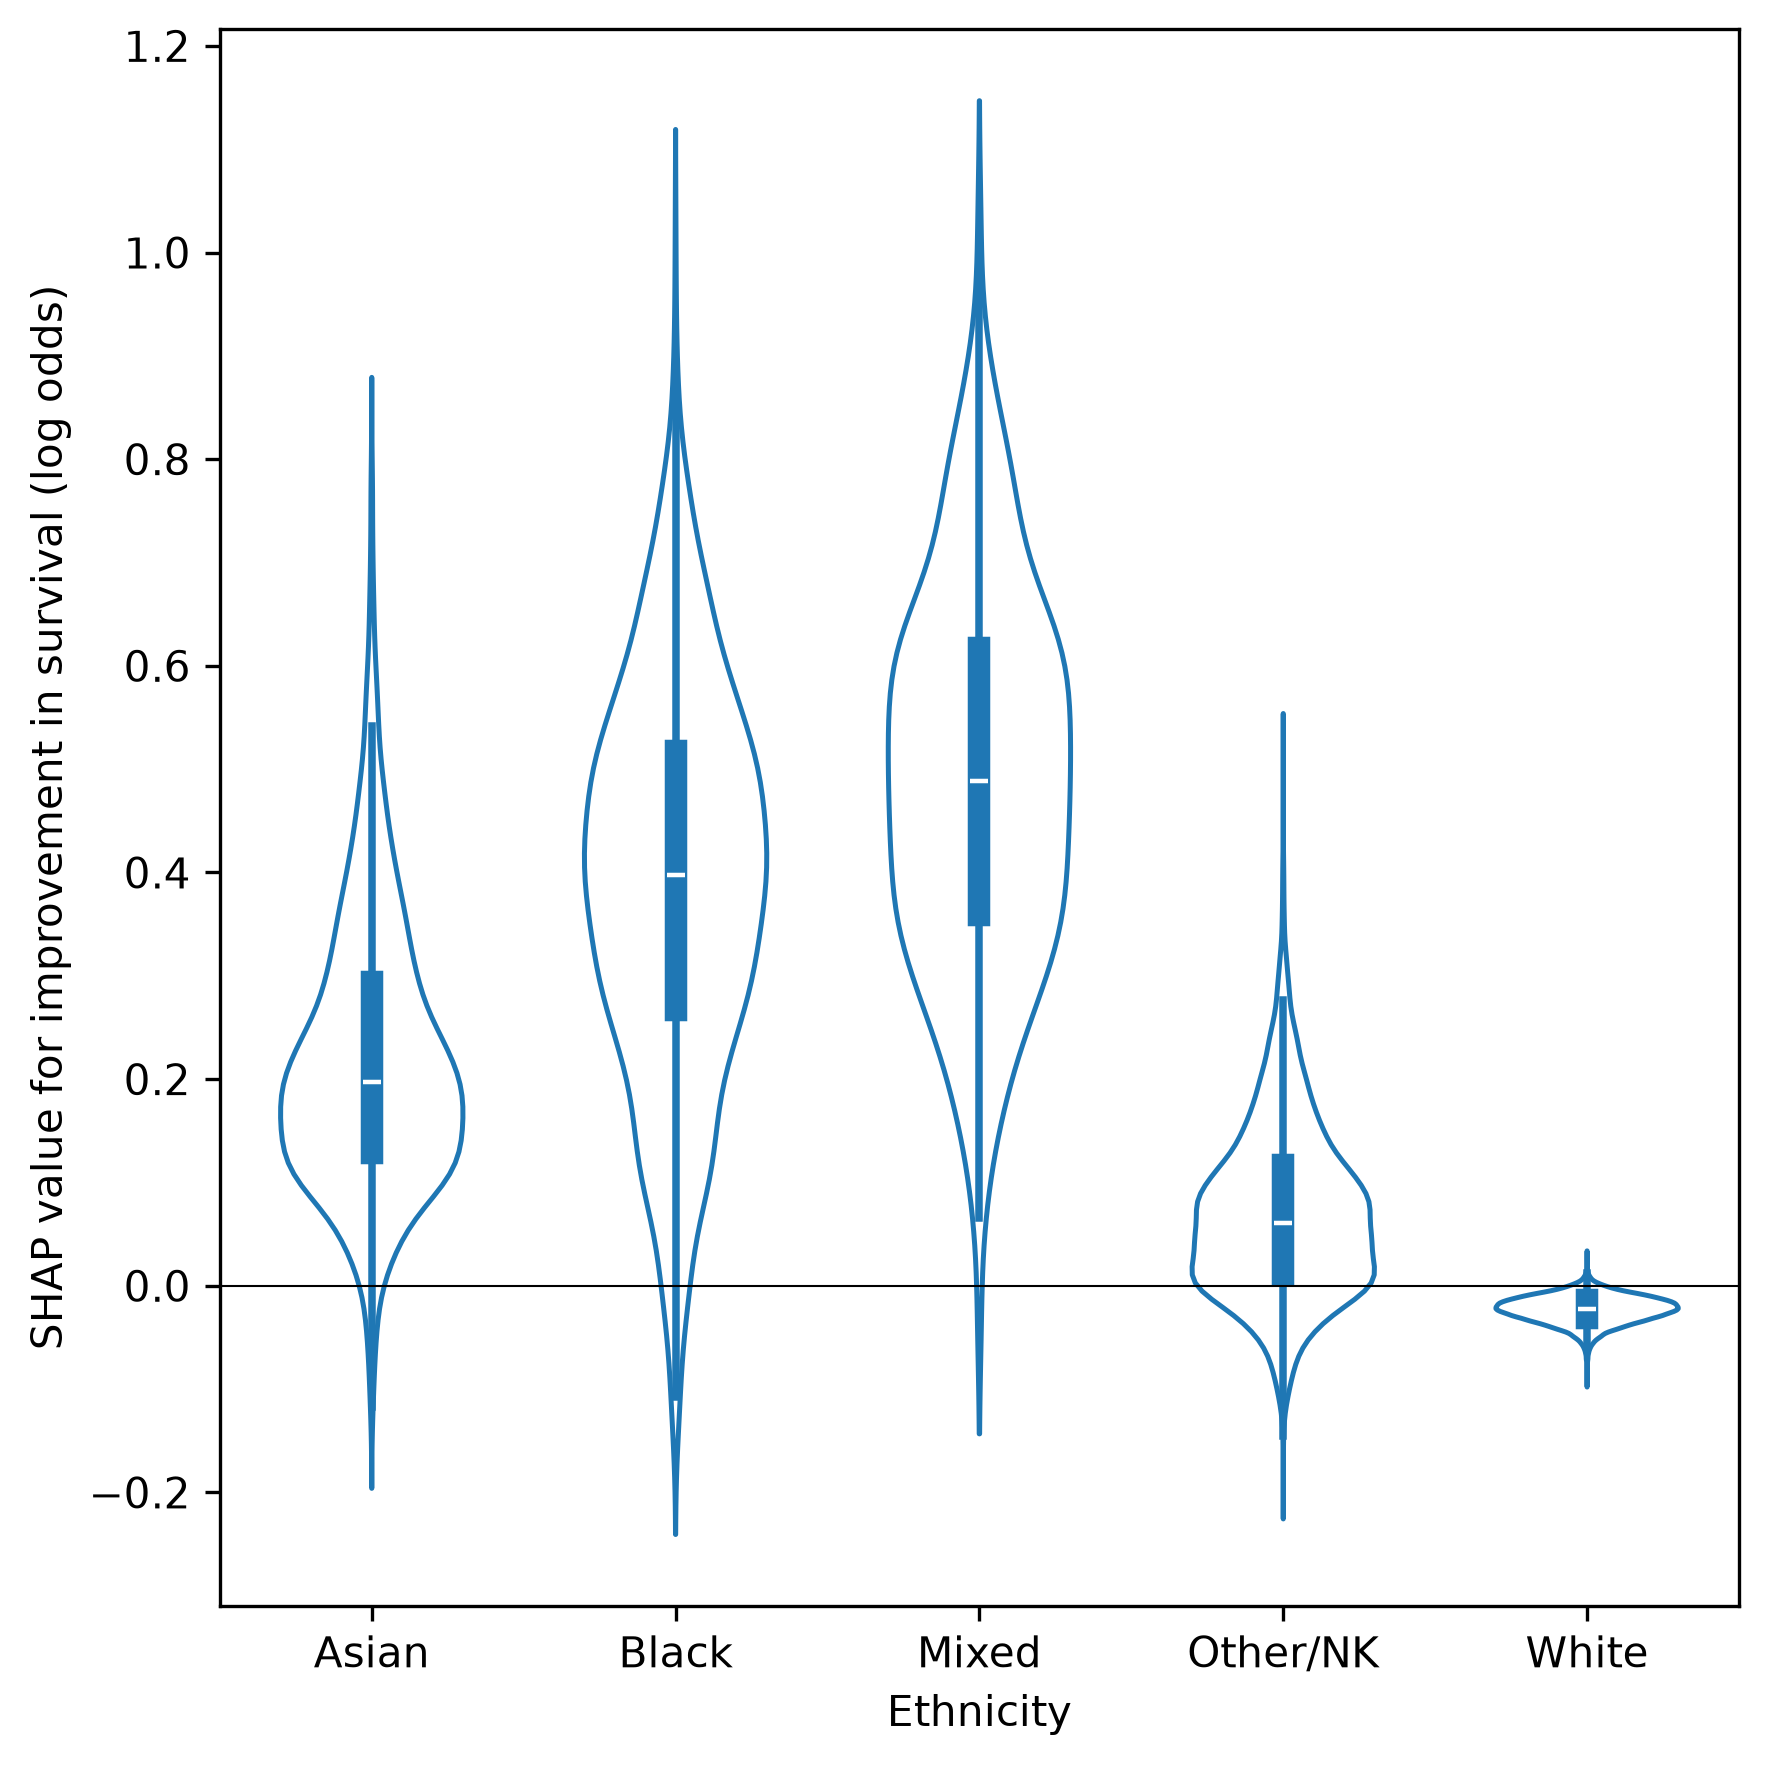
\includegraphics[width=\linewidth]{images/shap/shap_all_patients_survival_ethnicity.png}
        %\caption{}
    \end{subfigure}
    \hfill % Adds flexible horizontal spacing
    % Bottom right image (~55% width)
    \begin{subfigure}{0.543\textwidth}
        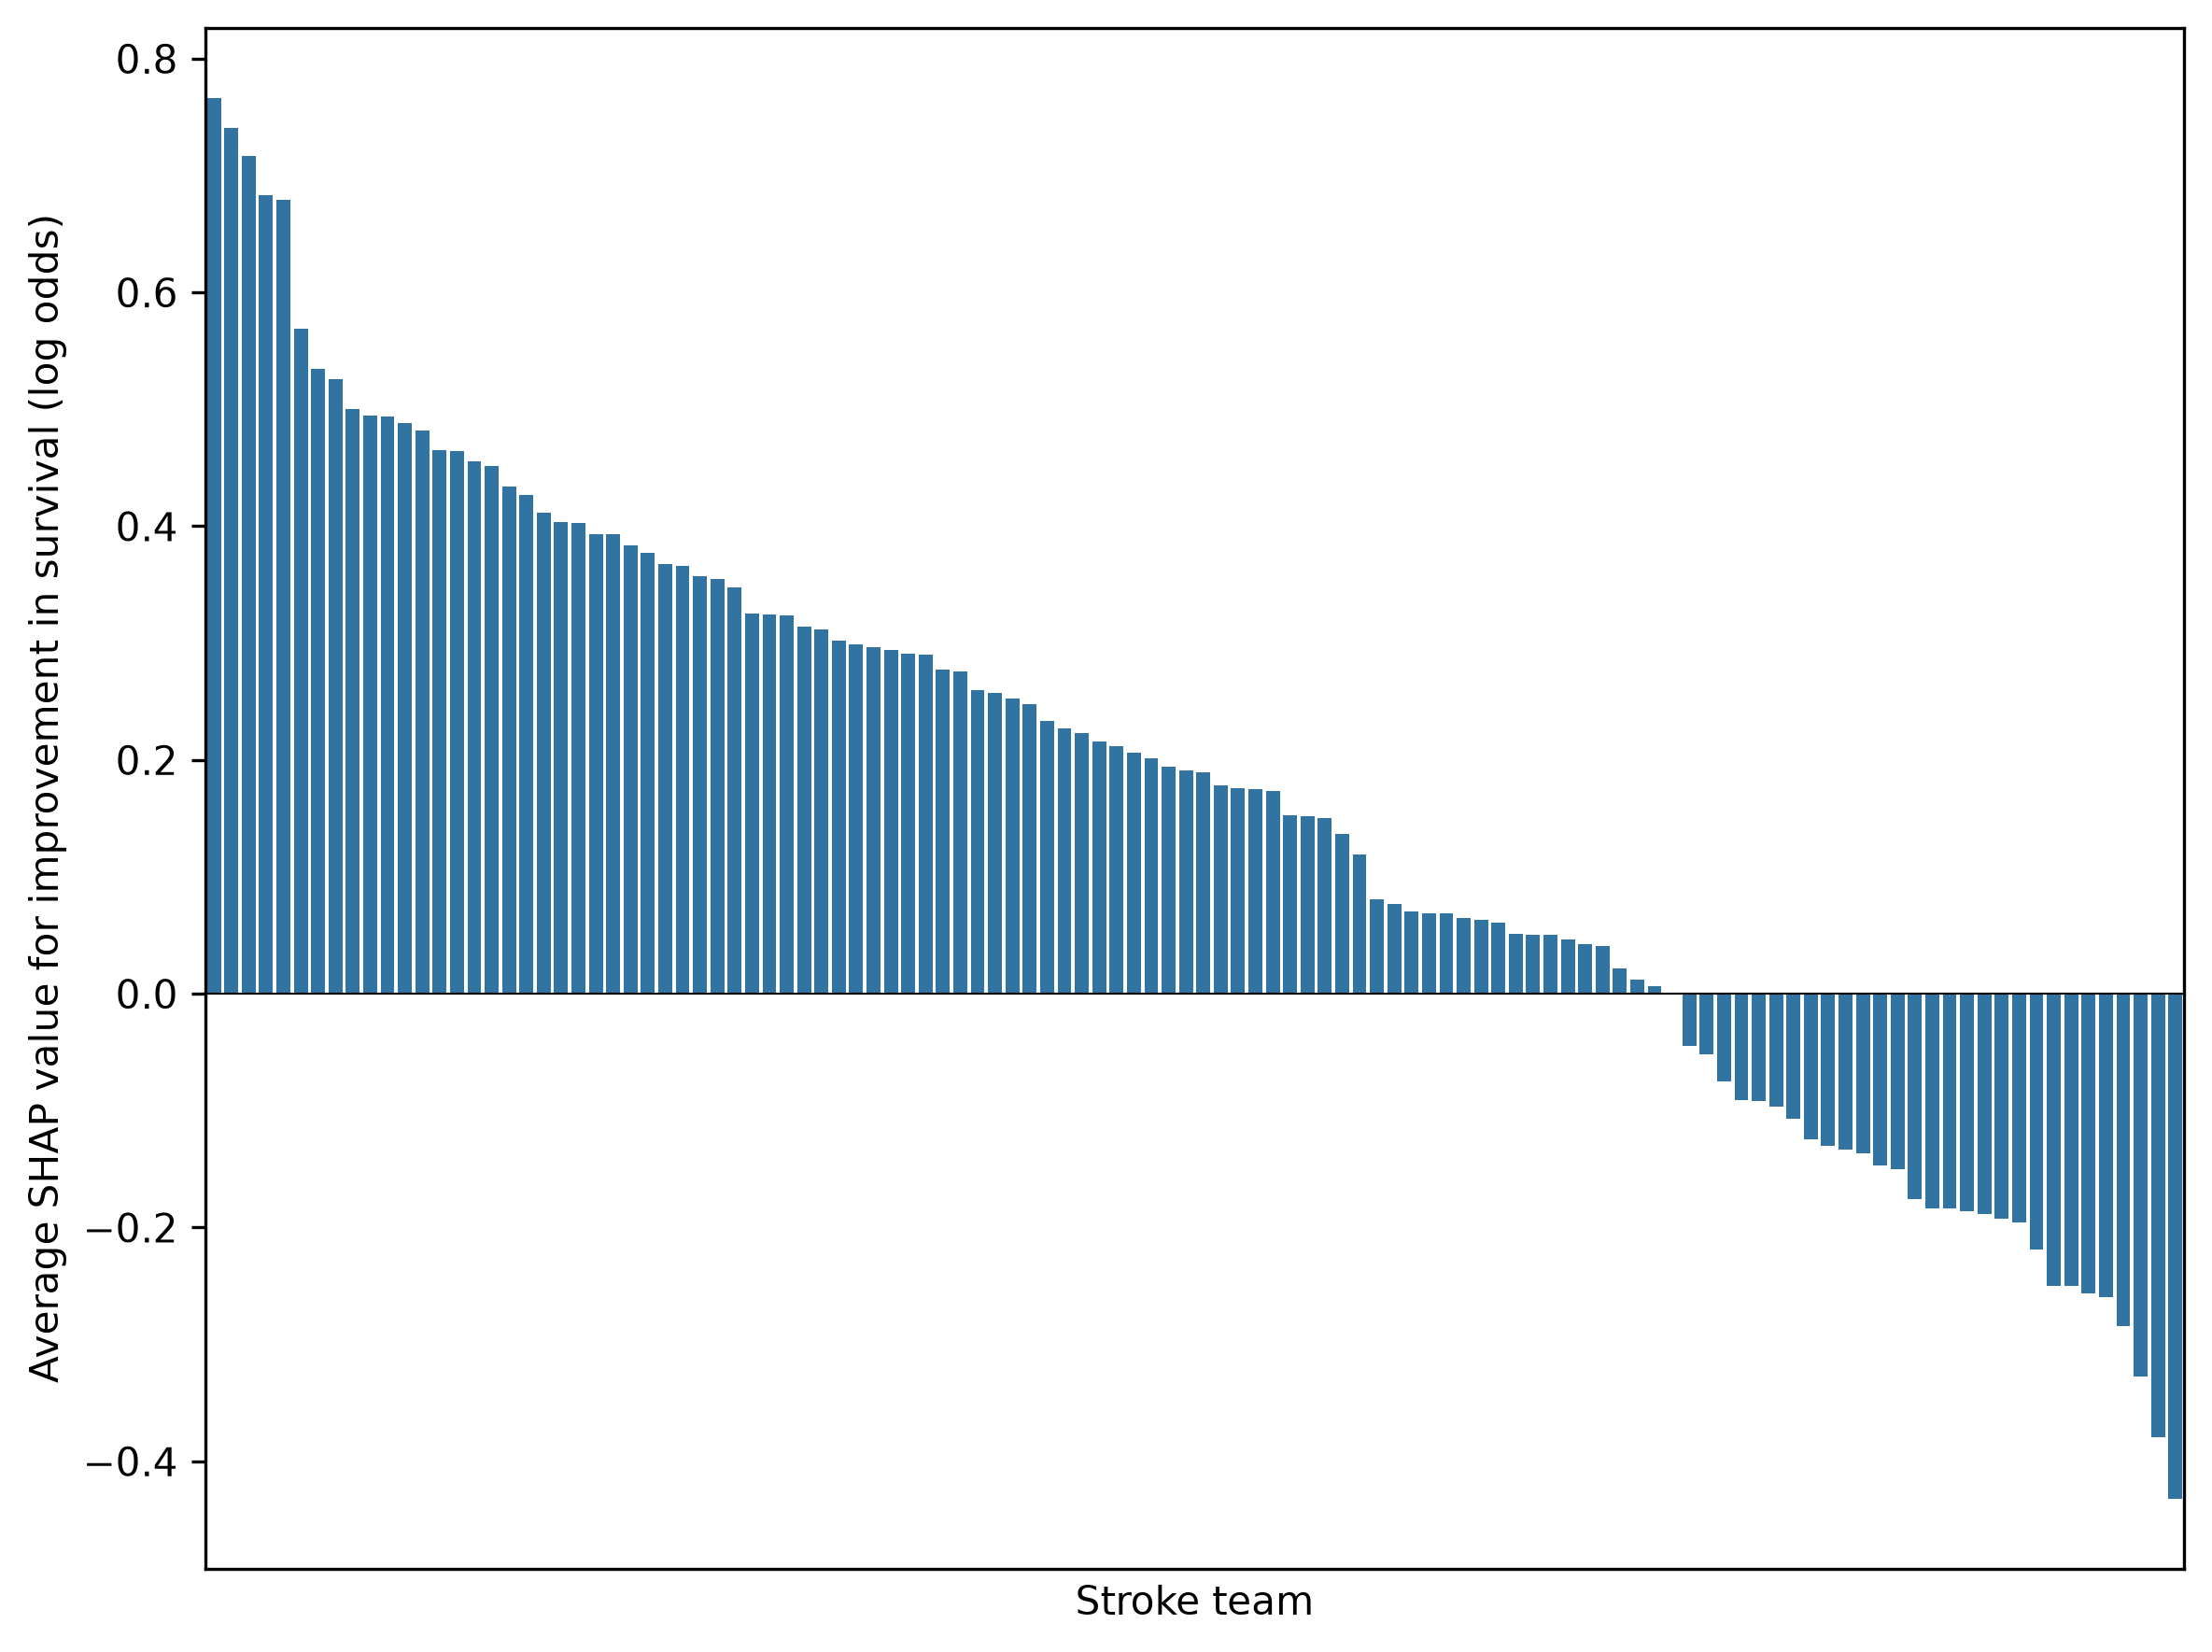
\includegraphics[width=\linewidth]{images/shap/shap_all_patients_survival_stroke_team.png}
        %\caption{}
    \end{subfigure}

    \caption{SHAP analysis of feature contributions to predicting survival in stroke patients. \textit{Top}: A SHAP summary plot detailing the impact of features on the model's log-odds predictions. Each point represents an individual patient instance. The position on the x-axis indicates the SHAP value, where positive values increase the predicted odds of survival, and negative values decrease it. For continuous and binary variables, colour represents the original feature value (red indicating high values; blue indicating low values). Categorical variables (\textit{stroke team} and \textit{ethnicity}) are plotted in grey. \textit{Bottom left}: Violin plots illustrating the distribution of SHAP values across distinct ethnic groups. This panel highlights the marginal impact and variance of ethnicity on the model’s prediction for survival. \textit{Bottom Right}: A ranked bar chart displaying the average SHAP value associated with each individual stroke team. This panel visualizes institutional variation, reflecting the contribution of the treating stroke team to the predicted survival outcome after accounting for patient-level clinical characteristics.}
    \label{fig:shap_survival_all}
\end{figure}

%% Untreated patients

\begin{figure}[htbp]
    \centering
    
    % Top image (Full width)
    \begin{subfigure}{0.50\textwidth}
        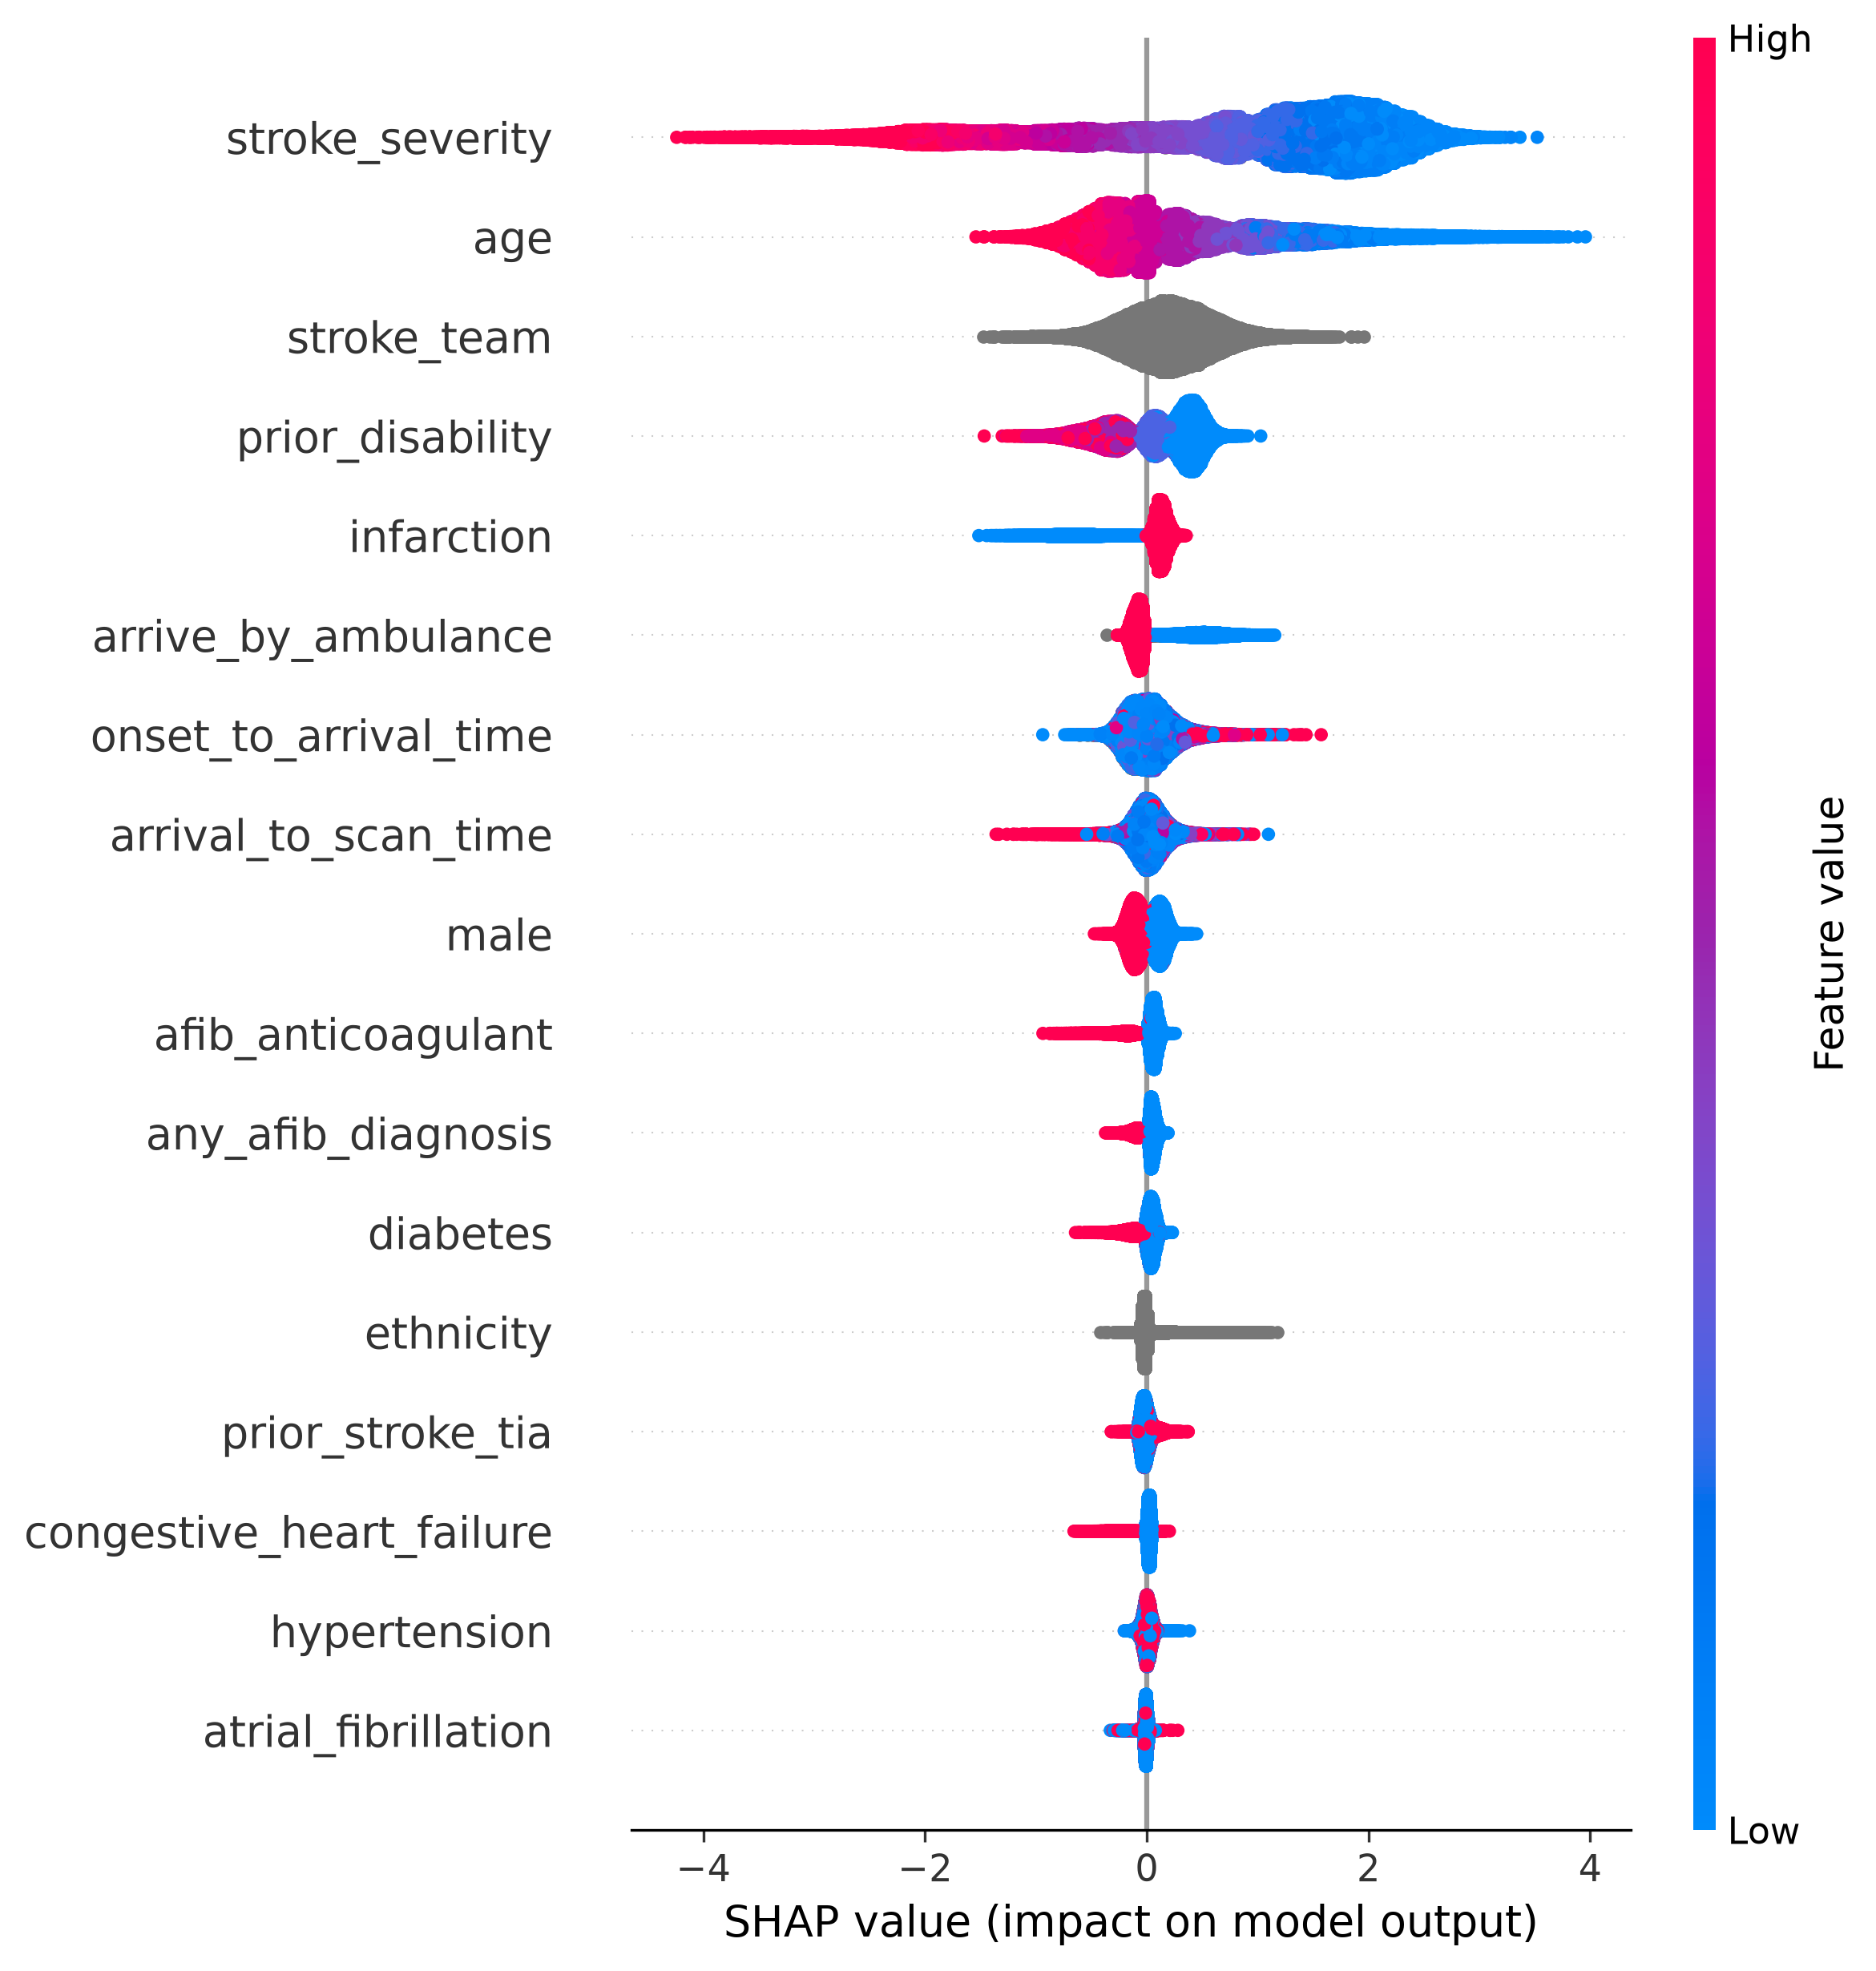
\includegraphics[width=\linewidth]{images/shap/shap_untreated_patients_survival.png}
        %\caption{}
    \end{subfigure}

    \vspace{0.5cm} % Optional vertical space between rows

    % Bottom left image (~45% width)
    \begin{subfigure}{0.407\textwidth}
        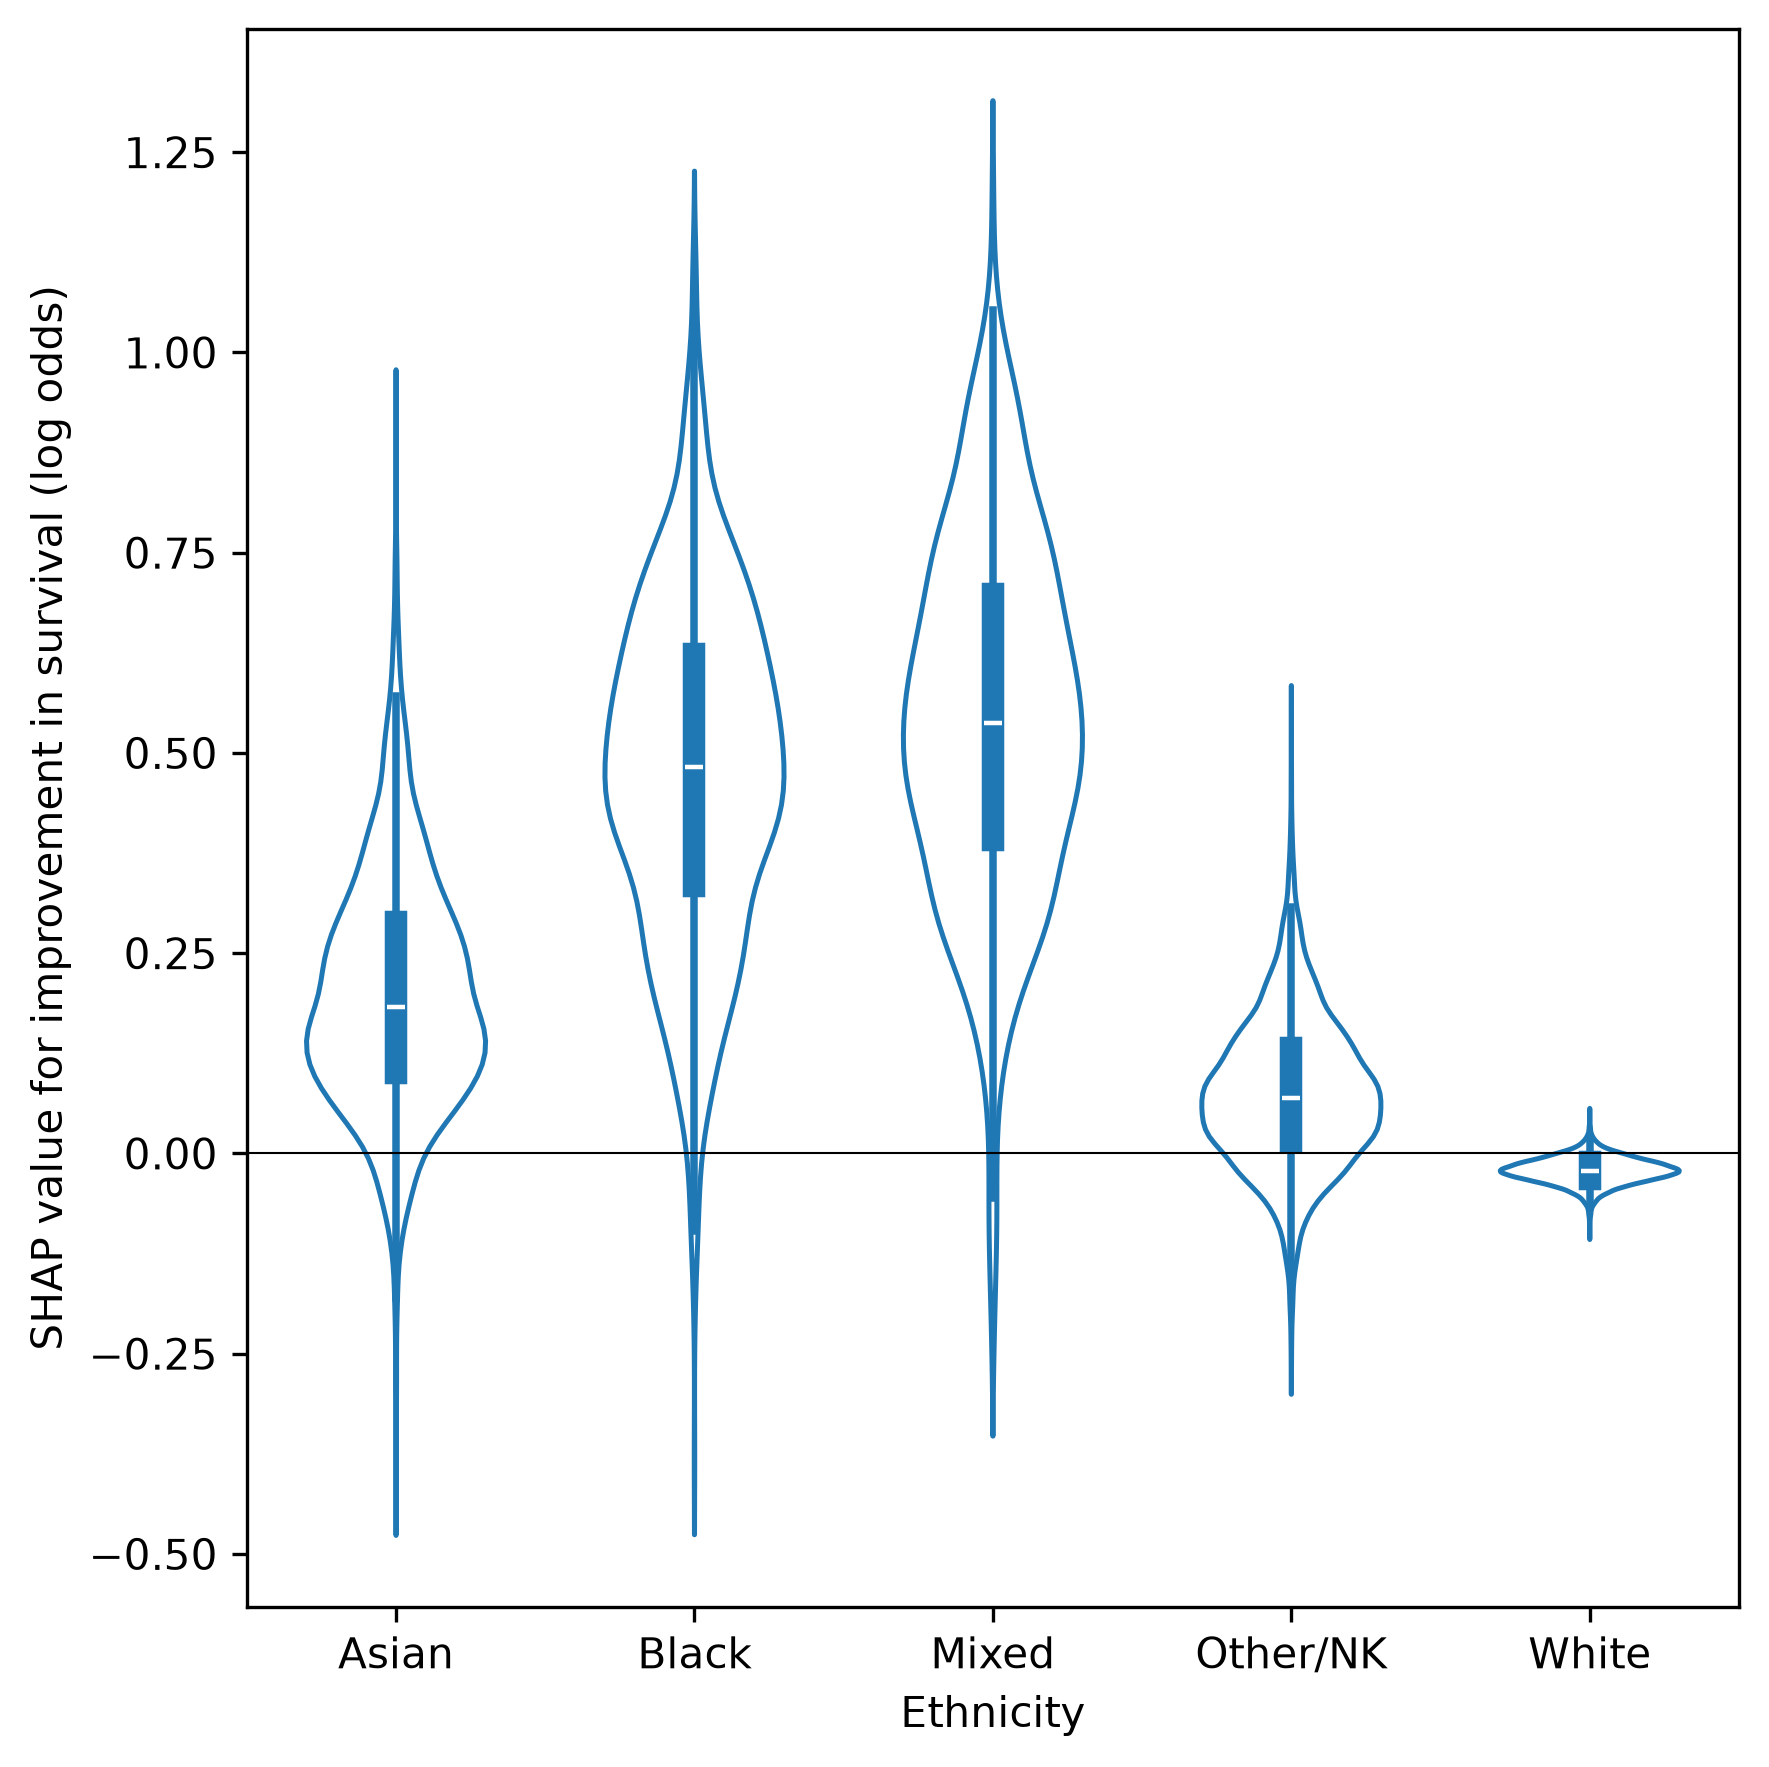
\includegraphics[width=\linewidth]{images/shap/shap_untreated_patients_survival_ethnicity.png}
        %\caption{}
    \end{subfigure}
    \hfill % Adds flexible horizontal spacing
    % Bottom right image (~55% width)
    \begin{subfigure}{0.543\textwidth}
        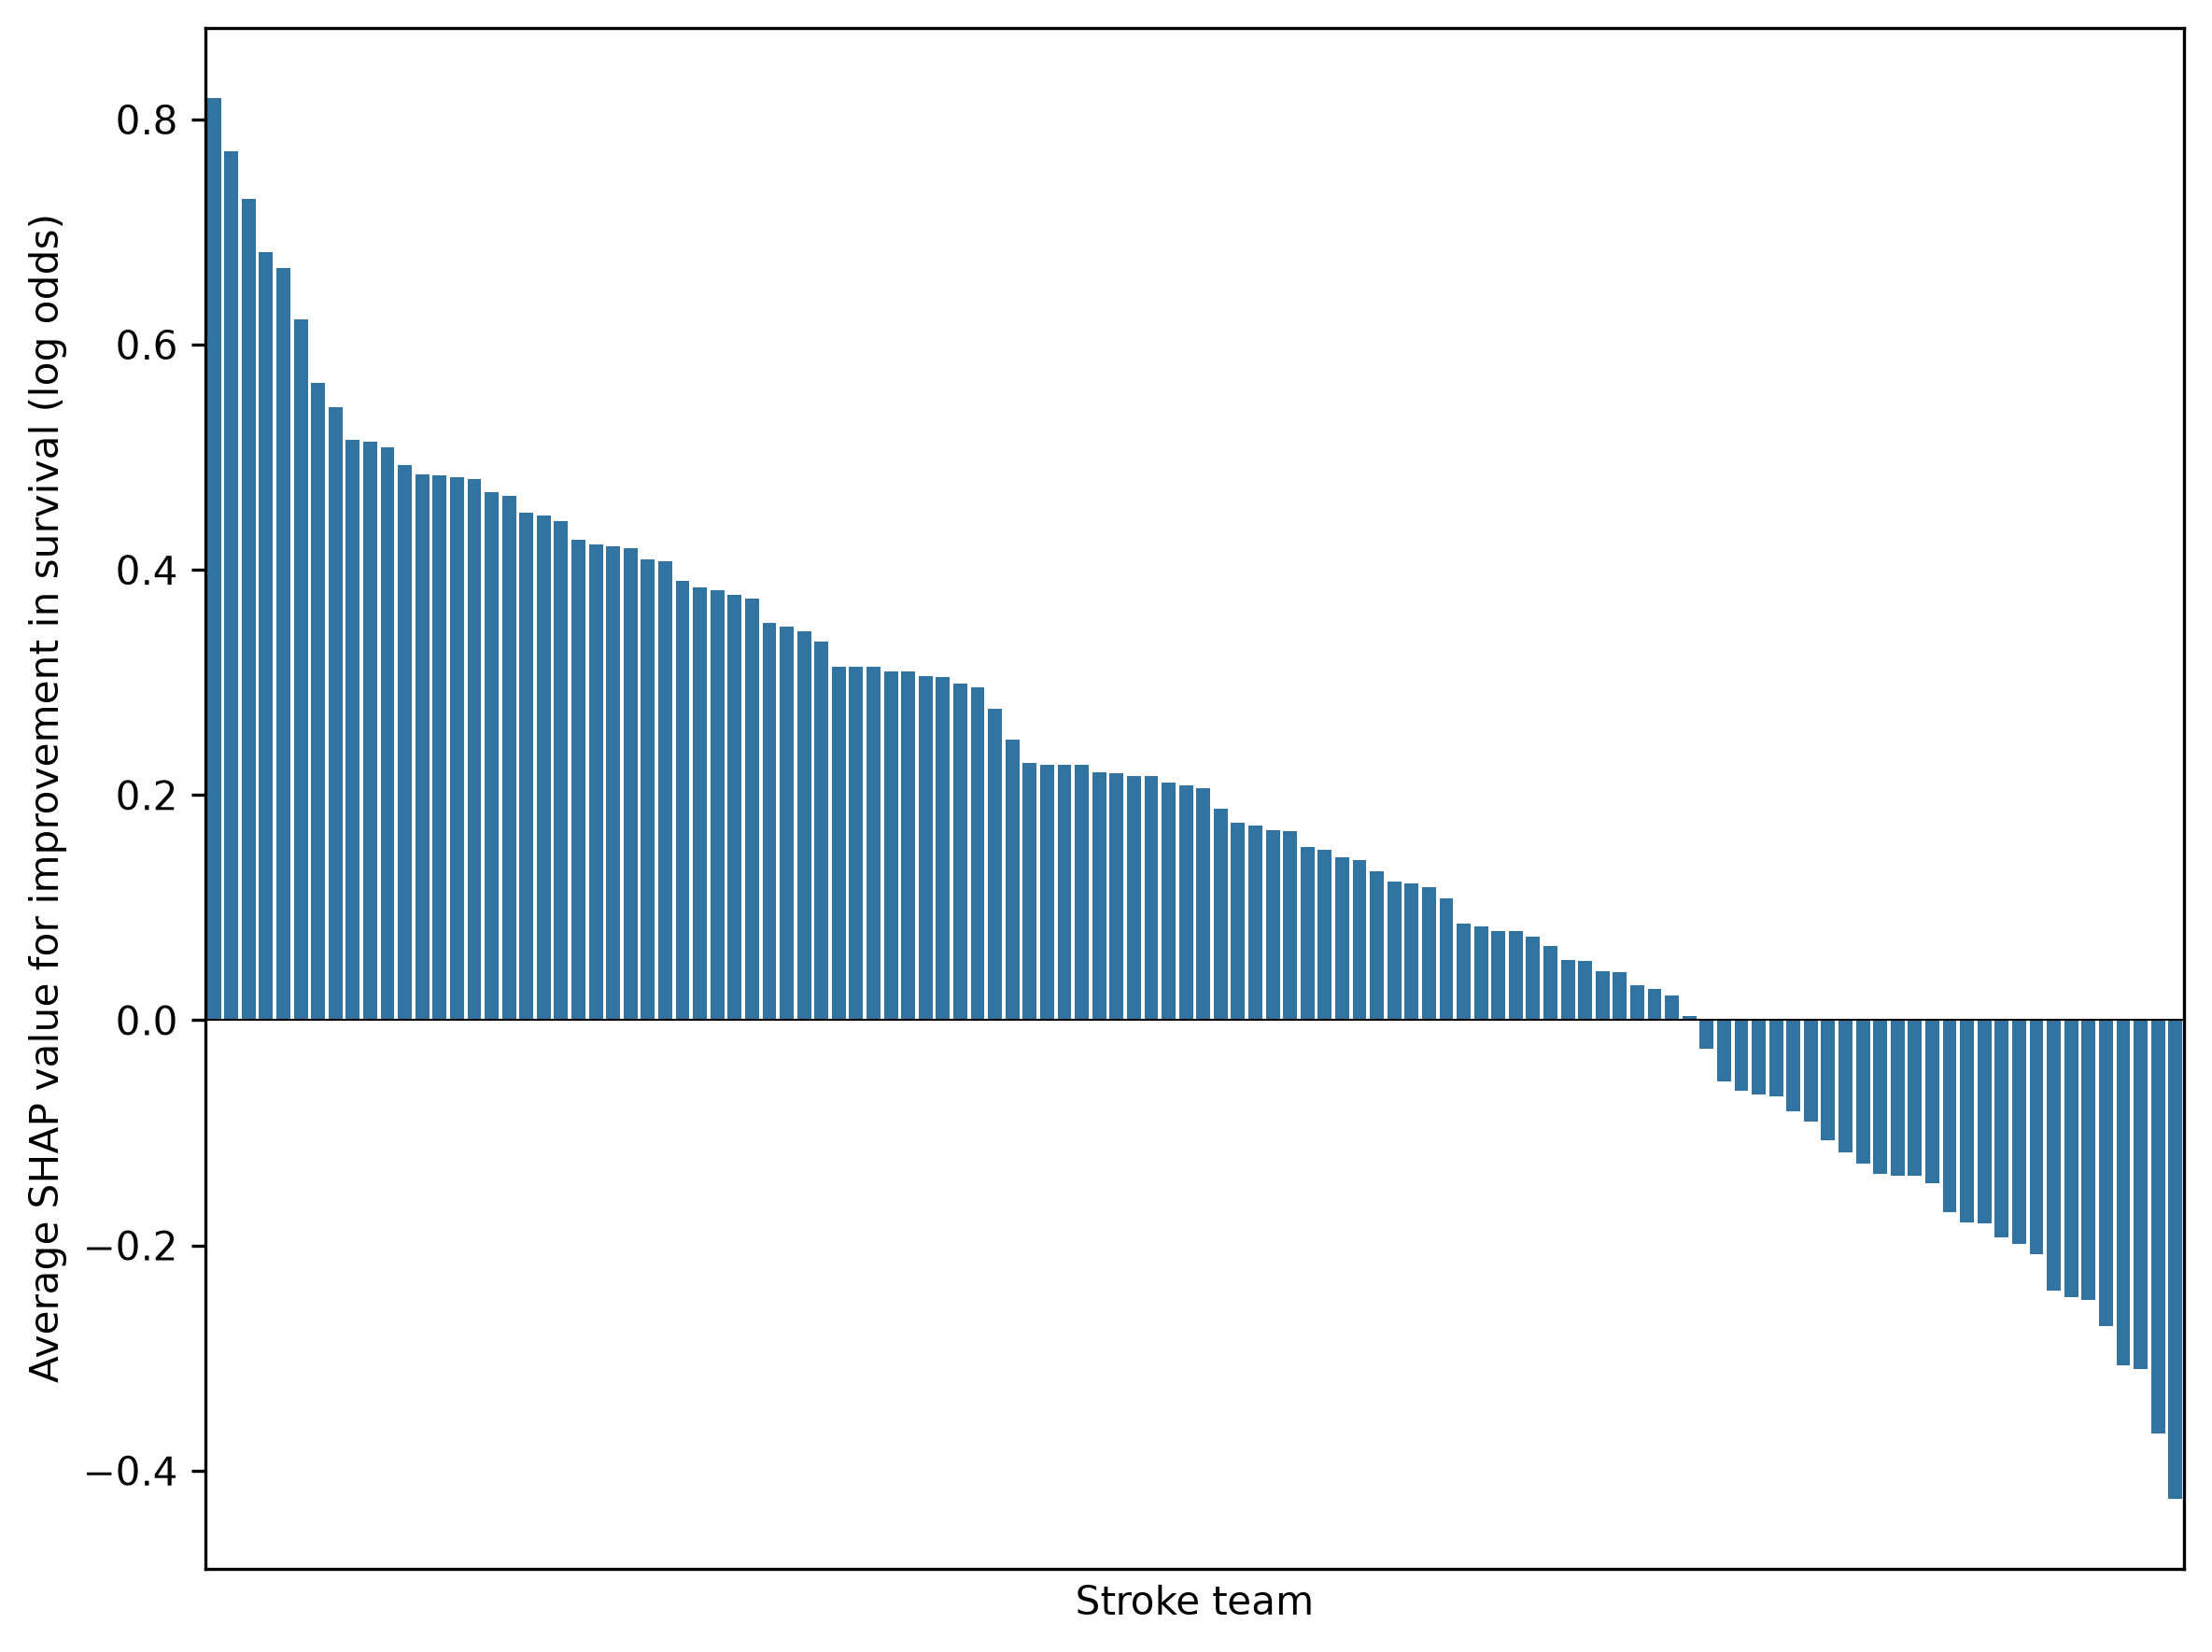
\includegraphics[width=\linewidth]{images/shap/shap_untreated_patients_survival_stroke_team.png}
        %\caption{}
    \end{subfigure}

    \caption{SHAP analysis of feature contributions to predicting survival in stroke patients who did not receive thrombolysis or thrombectomy. \textit{Top}: A SHAP summary plot detailing the impact of features on the model's log-odds predictions. Each point represents an individual patient instance. The position on the x-axis indicates the SHAP value, where positive values increase the predicted odds of survival, and negative values decrease it. For continuous and binary variables, colour represents the original feature value (red indicating high values; blue indicating low values). Categorical variables (\textit{stroke team} and \textit{ethnicity}) are plotted in grey. \textit{Bottom left}: Violin plots illustrating the distribution of SHAP values across distinct ethnic groups. This panel highlights the marginal impact and variance of ethnicity on the model’s prediction for survival. \textit{Bottom Right}: A ranked bar chart displaying the average SHAP value associated with each individual stroke team. This panel visualizes institutional variation, reflecting the contribution of the treating stroke team to the predicted survival outcome after accounting for patient-level clinical characteristics.}
    \label{fig:shap_survival_no_treatment}
\end{figure}

%%%%%%%%%%%%%%%%%%%%%%%%%% Length of stay %%%%%%%%%%%%%%%%%%%%%%%%%%%%%

%% All patients

\begin{figure}[htbp]
    \centering
    
    % Top image (Full width)
    \begin{subfigure}{0.50\textwidth}
        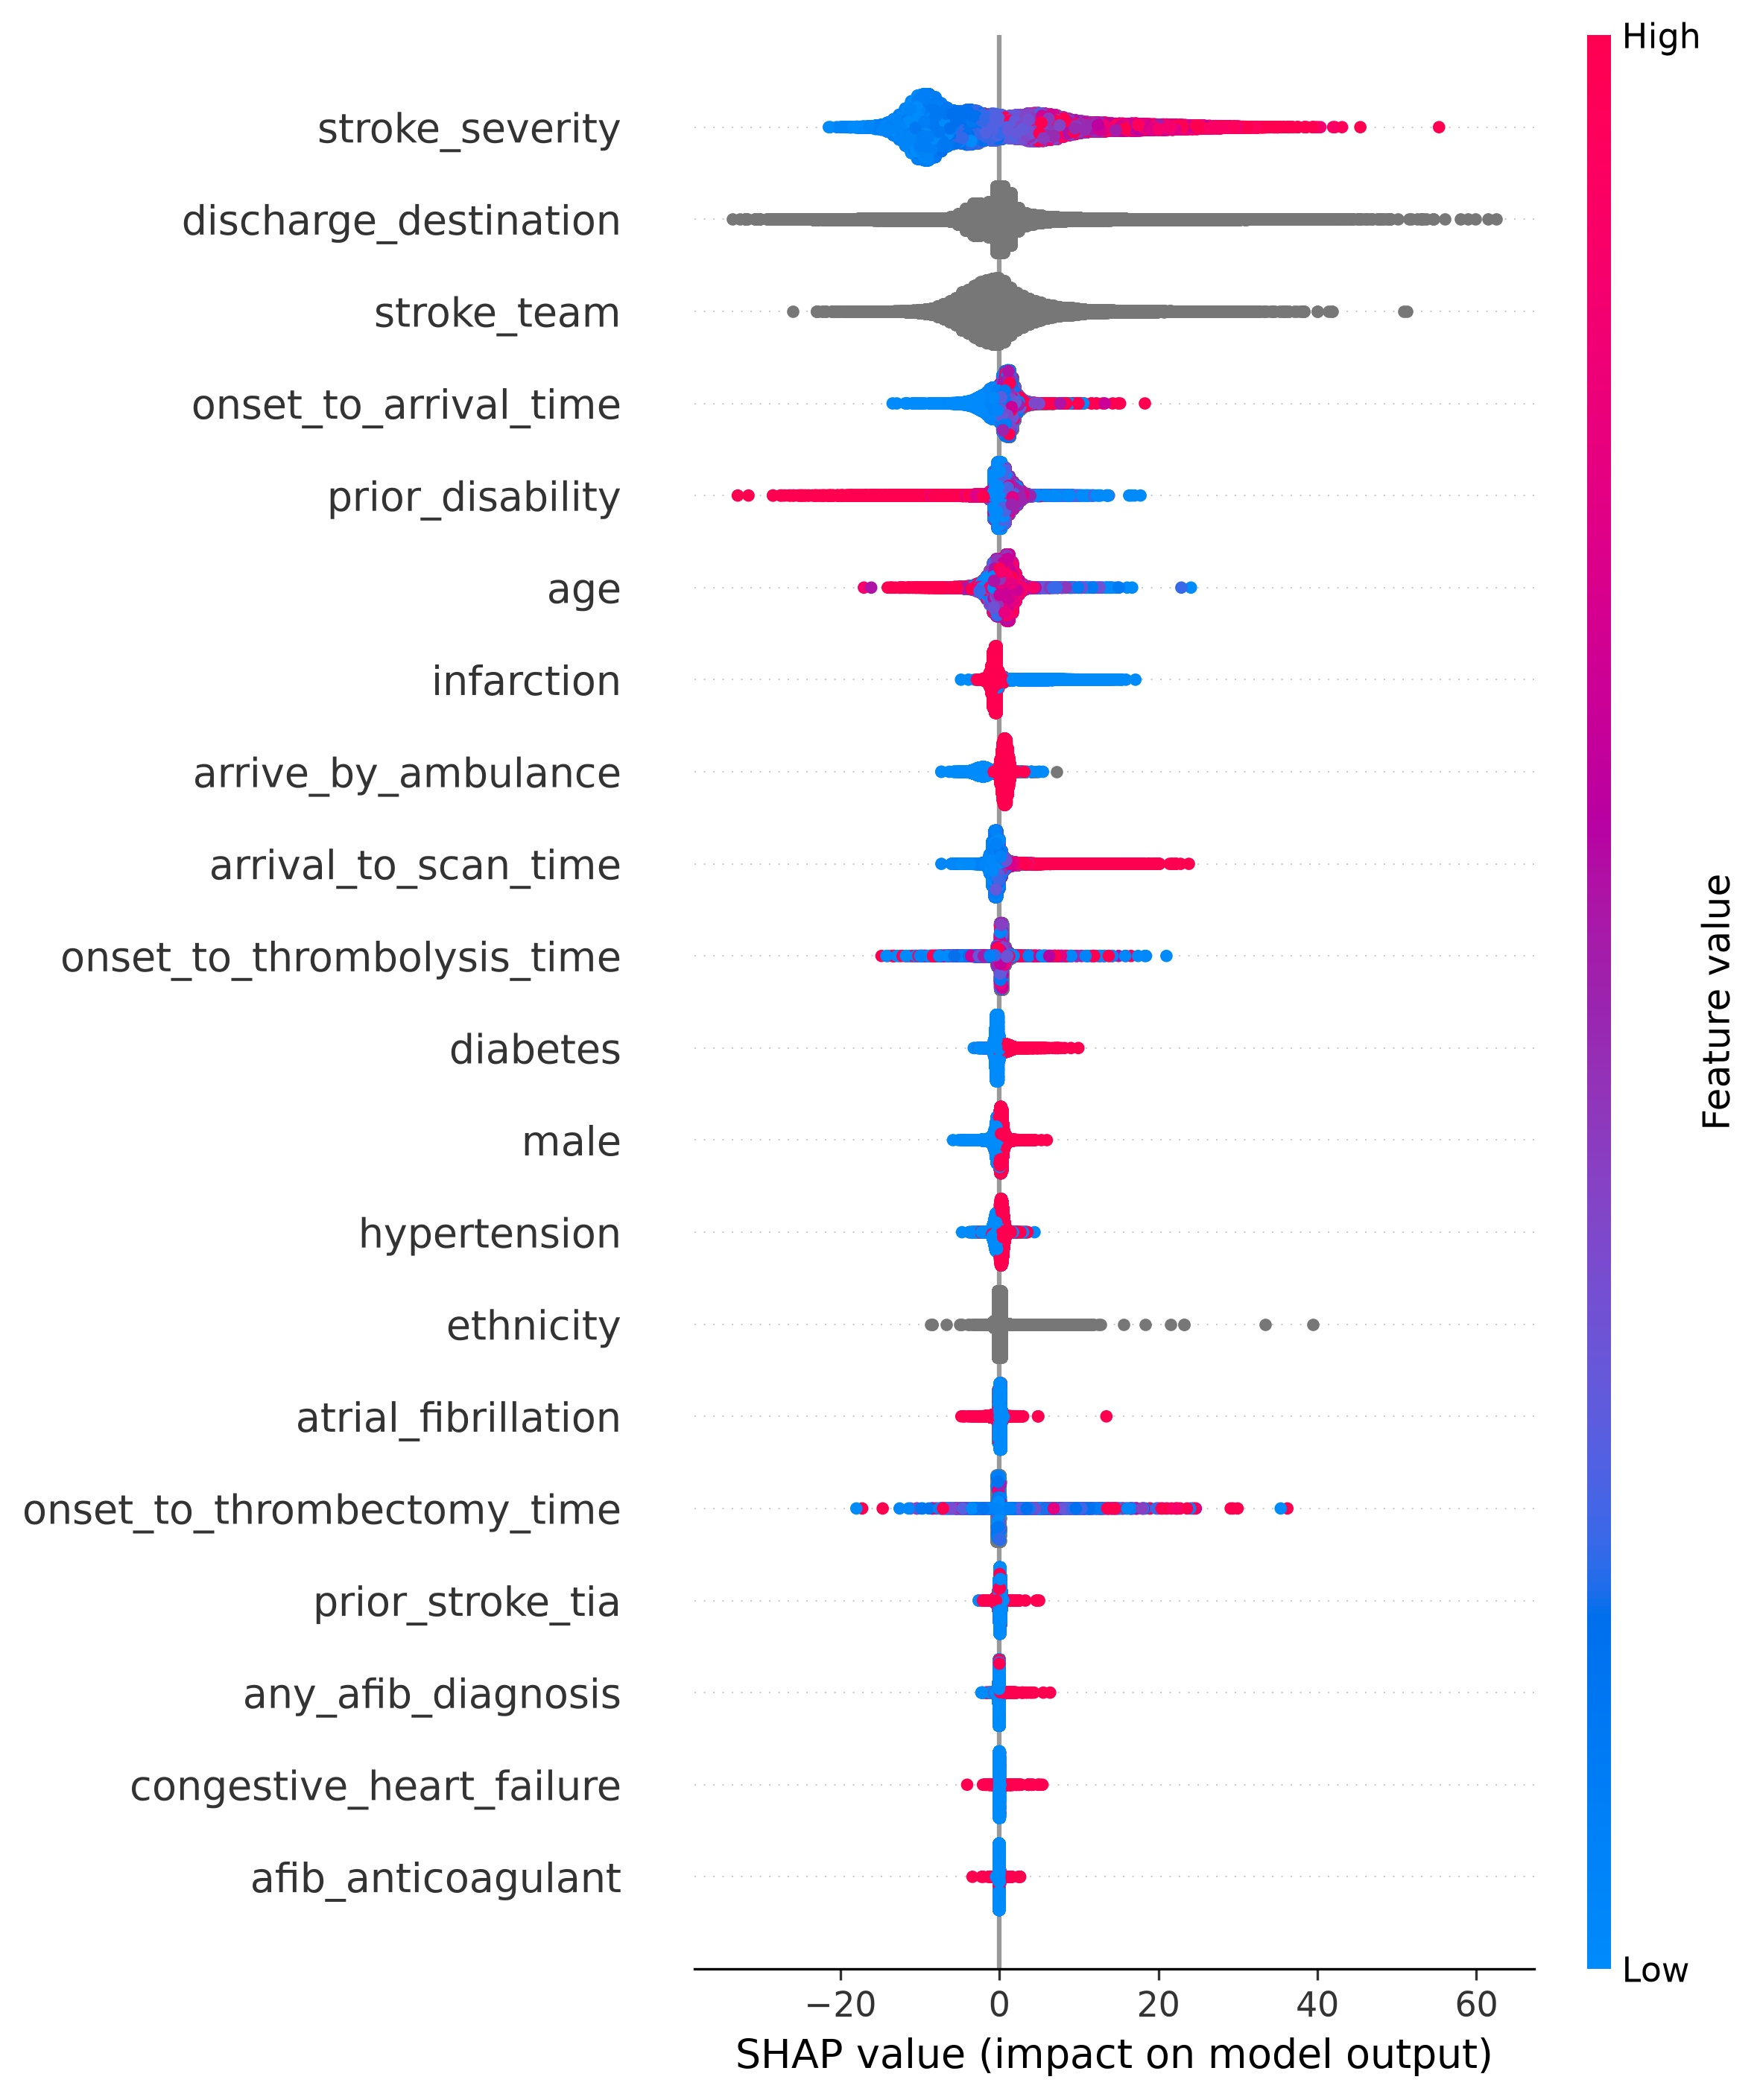
\includegraphics[width=\linewidth]{images/shap/shap_all_patients_los.png}
        %\caption{}
    \end{subfigure}

    \vspace{0.5cm} % Optional vertical space between rows

    % Bottom left image (~45% width)
    \begin{subfigure}{0.24\textwidth}
        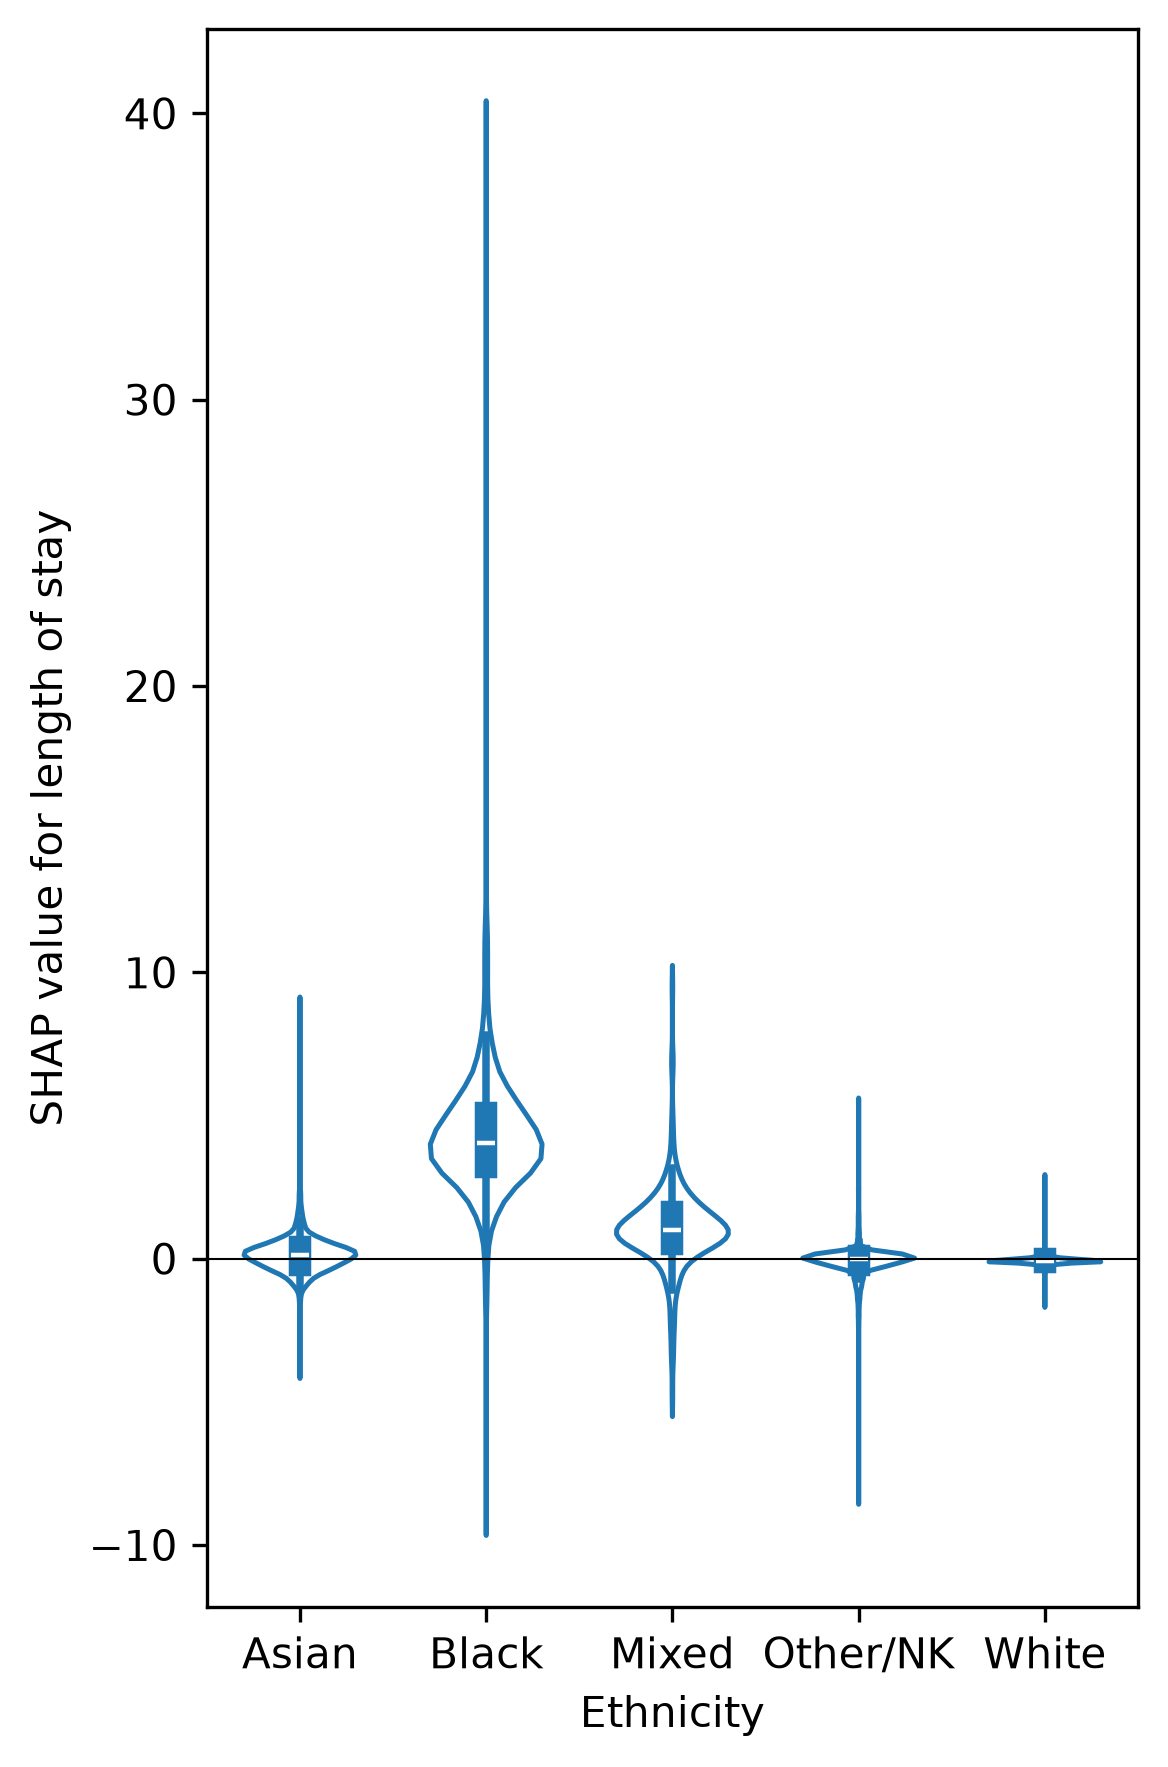
\includegraphics[width=\linewidth]{images/shap/shap_all_patients_los_ethnicity.png}
        %\caption{}
    \end{subfigure}
    \hfill % Adds flexible horizontal spacing
        \begin{subfigure}{0.24\textwidth}
        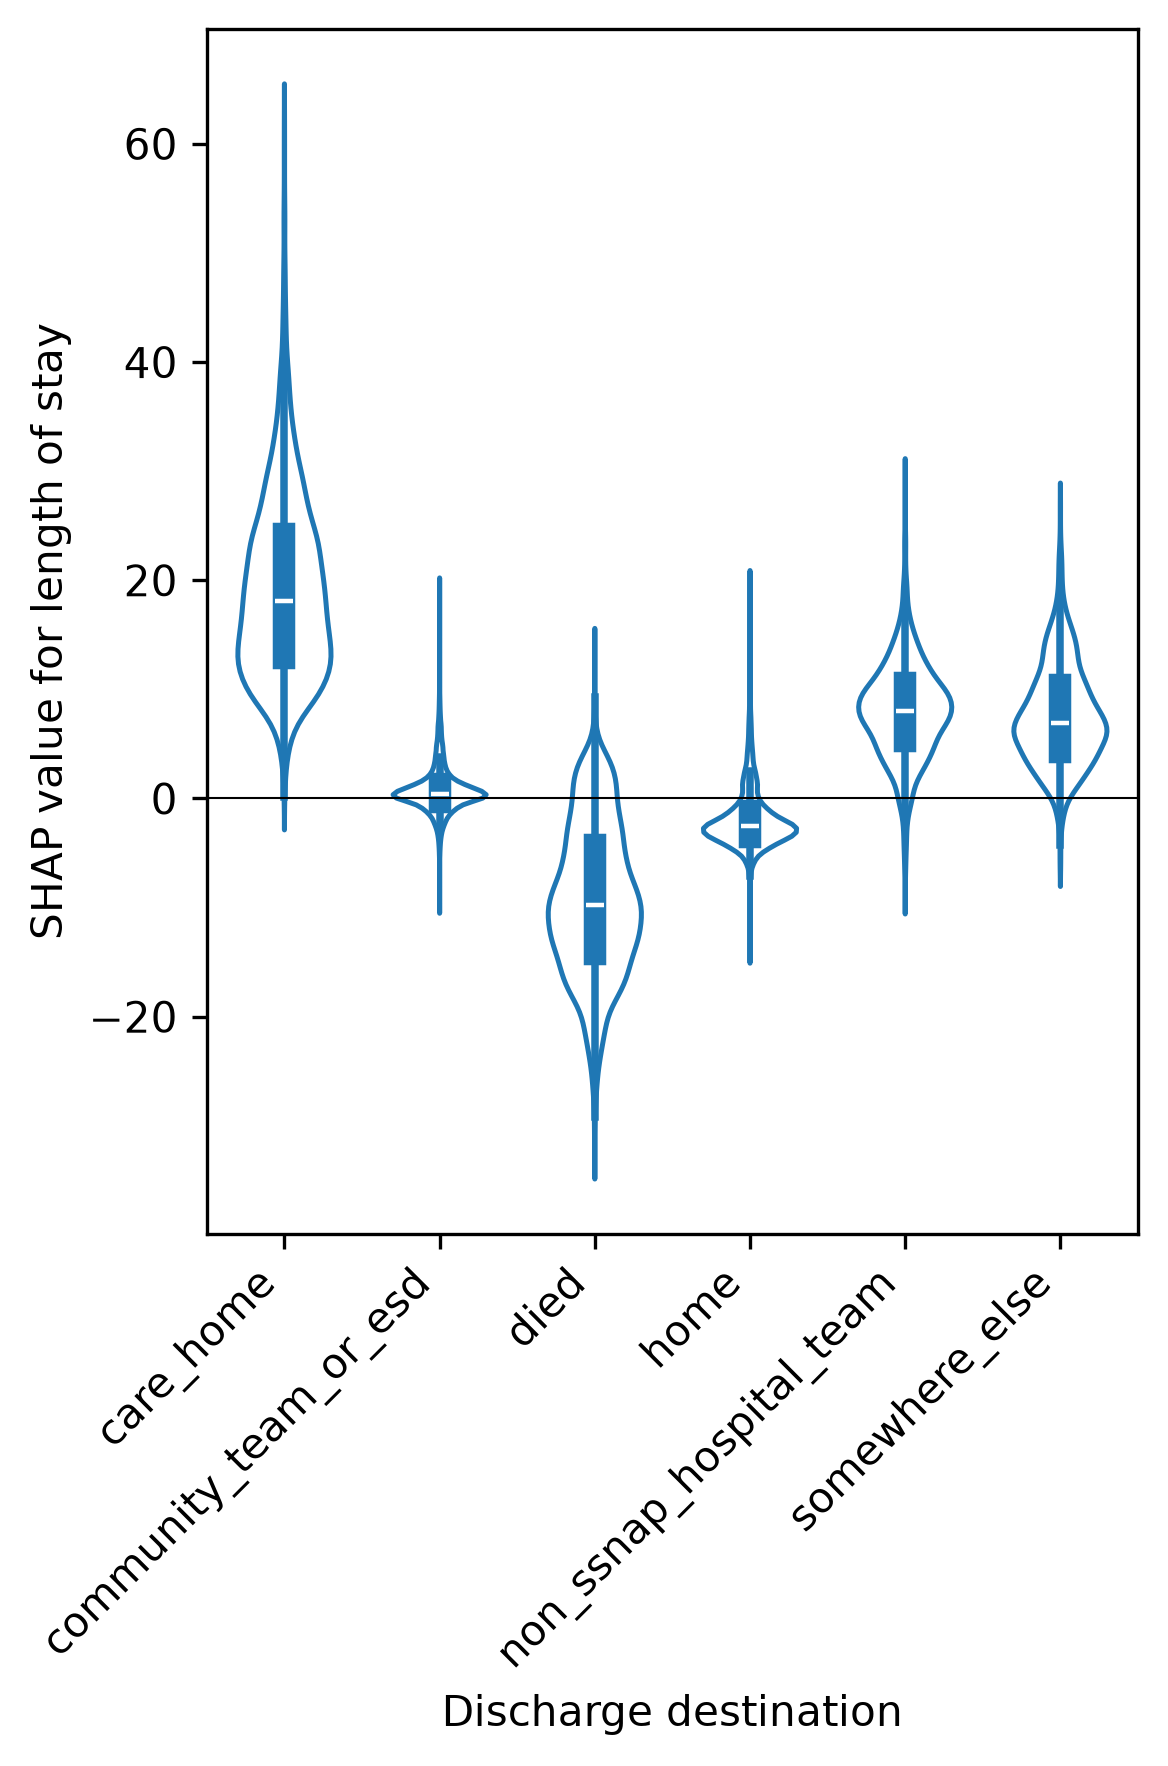
\includegraphics[width=\linewidth]{images/shap/shap_all_patients_los_discharge_destination.png}
        %\caption{}
        \label{fig:bottom-middke}
    \end{subfigure}
    \hfill
    % Bottom right image (~55% width)
    \begin{subfigure}{0.49\textwidth}
        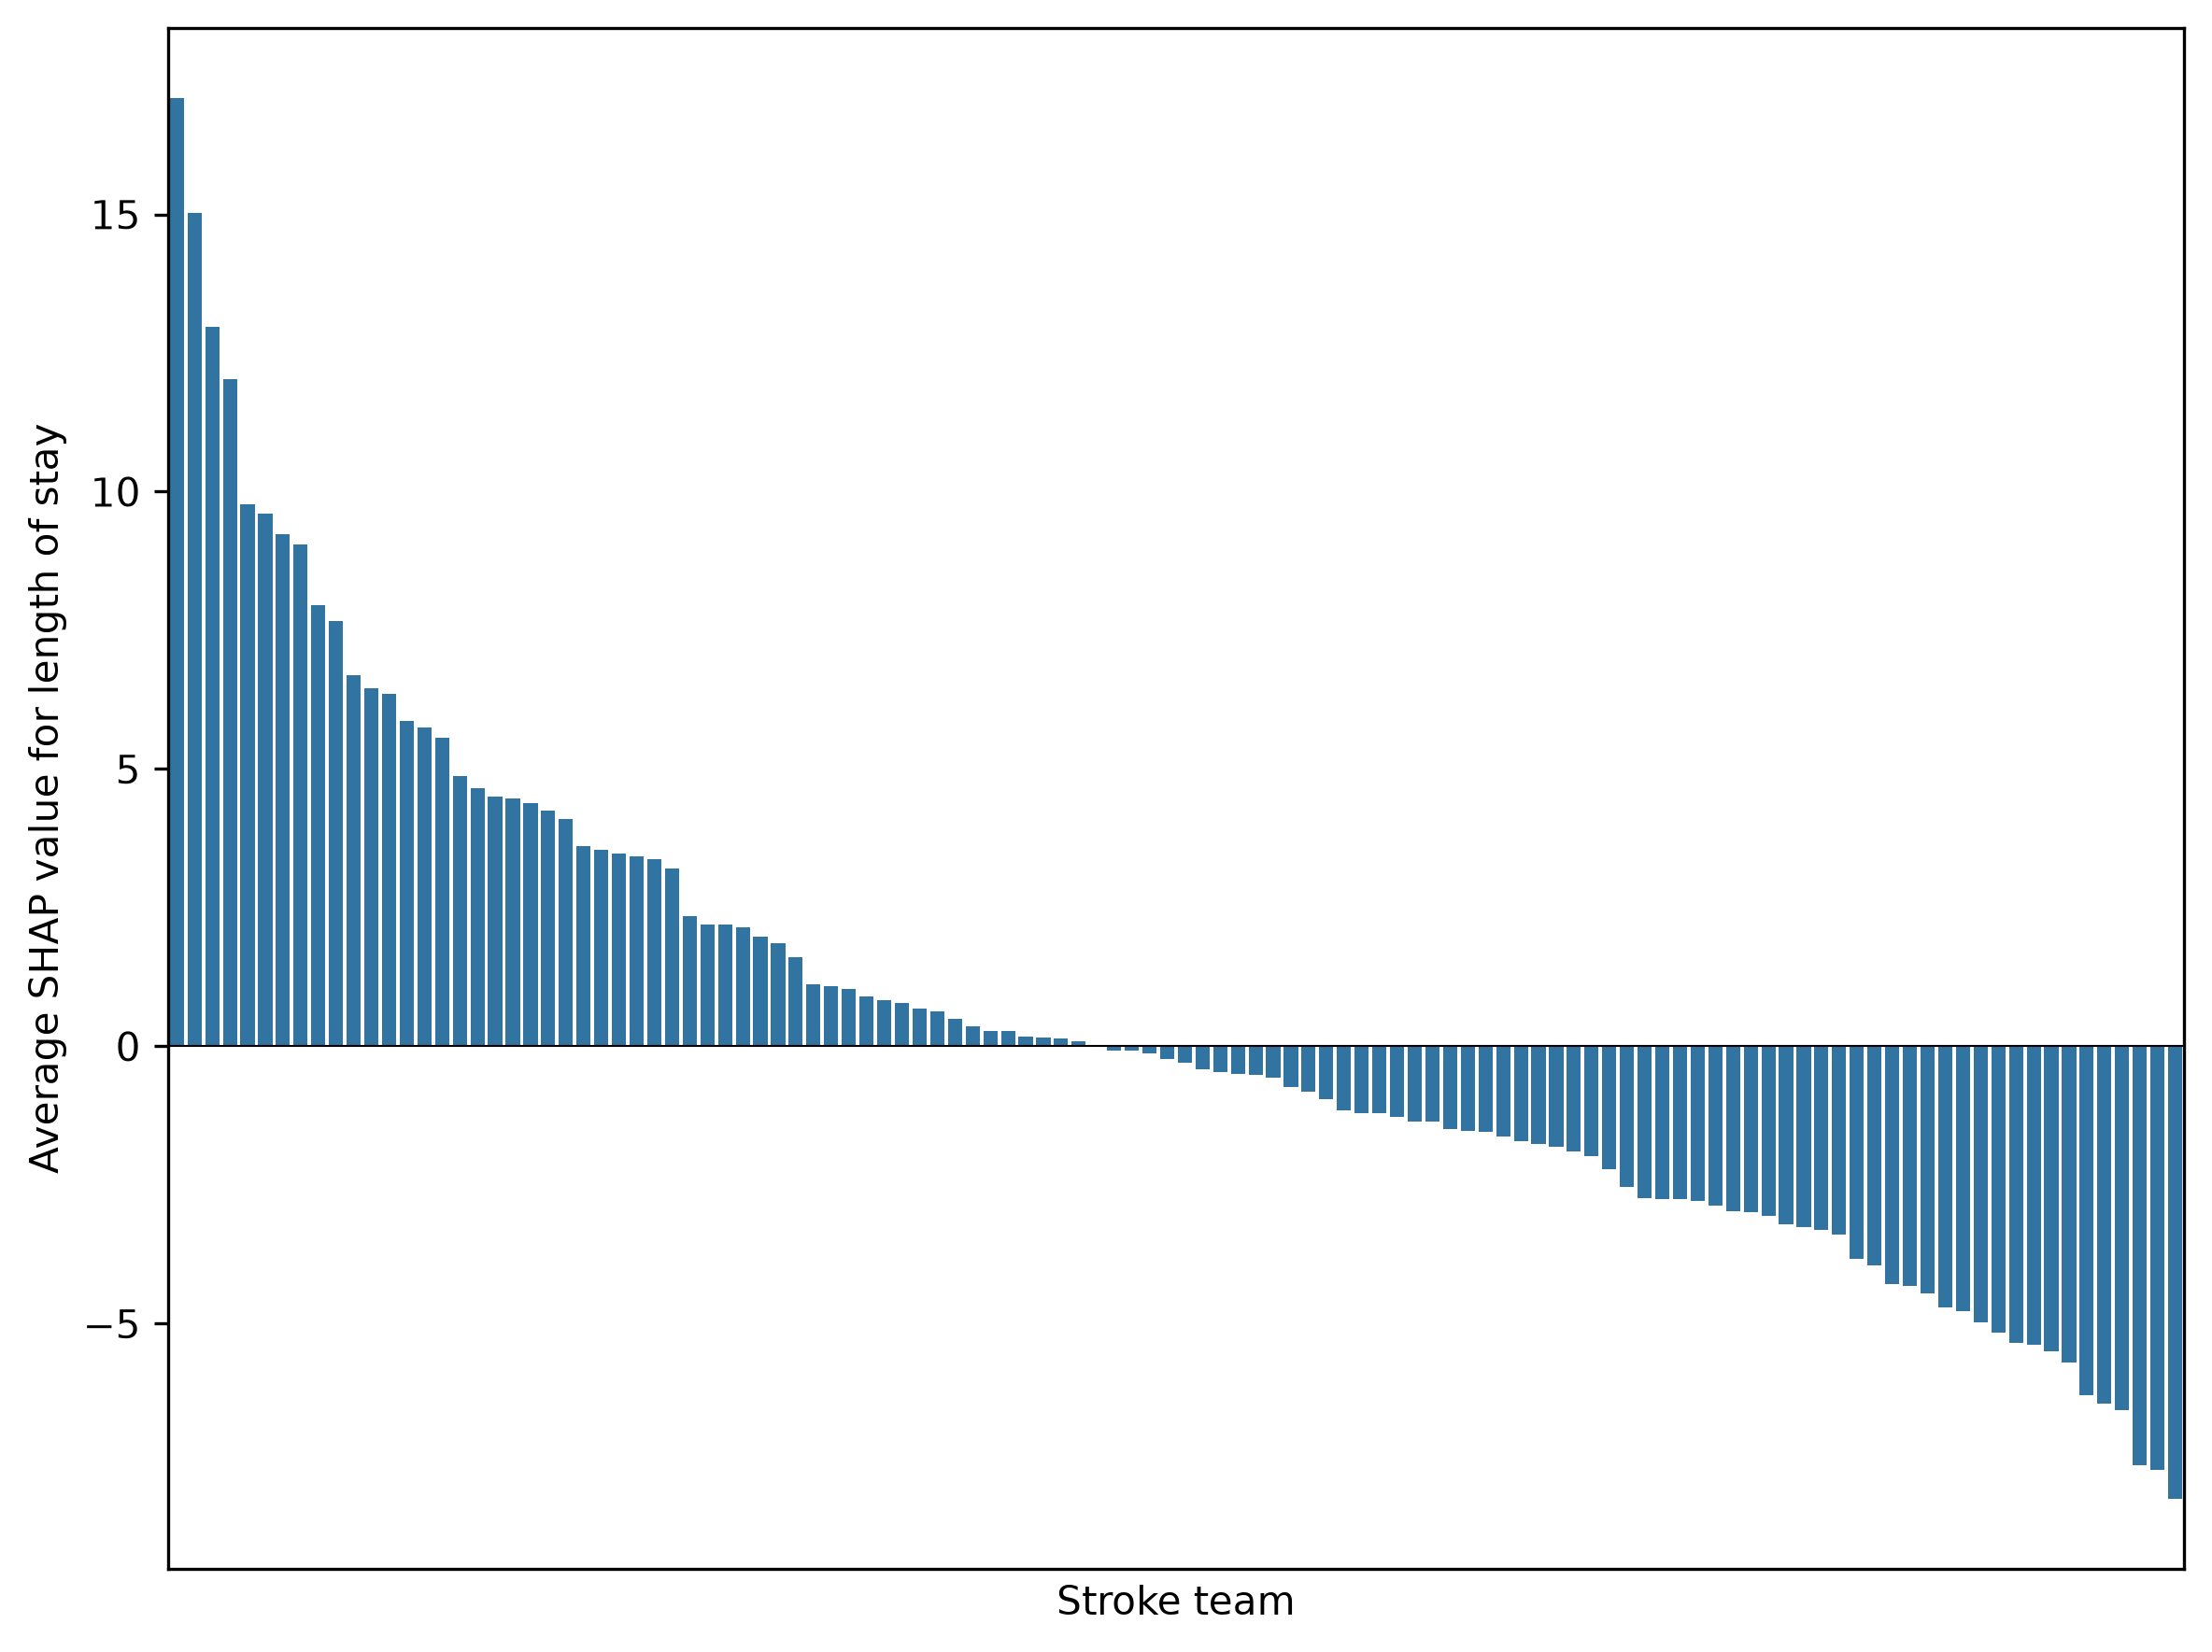
\includegraphics[width=\linewidth]{images/shap/shap_all_patients_los_stroke_team.png}
        %\caption{}
    \end{subfigure}

    \caption{SHAP analysis of feature contributions to predicting length of stay for stroke patients. \textit{Top}: A SHAP summary plot detailing feature impacts on the model's predictions. Each point represents an individual patient. The x-axis indicates the SHAP value, where positive values increase the predicted length of stay, and negative values decrease it. For continuous and binary variables, colour represents the original feature value (red for high; blue for low). Categorical variables (\textit{stroke team} and \textit{ethnicity}) are plotted in grey. \textit{Bottom left and middle}: Violin plots illustrating the distribution of SHAP values across ethnic groups and by discharge destination, highlighting the marginal impact of ethnicity and discharge destination on the predicted length of stay. \textit{Bottom right}: A ranked bar chart displaying the average SHAP value for each stroke team. This visualizes institutional variation, reflecting the treating stroke team's contribution to the length of stay after accounting for patient-level clinical characteristics.}
    \label{fig:shap_los_all}
\end{figure}

%%%%%%%%%%%%%%%%%%%% Use of thrombolysis %%%%%%%%%%%%%%%%%%%%%%%%

\begin{figure}[htbp]
    \centering
    
    % Top image (Full width)
    \begin{subfigure}{0.50\textwidth}
        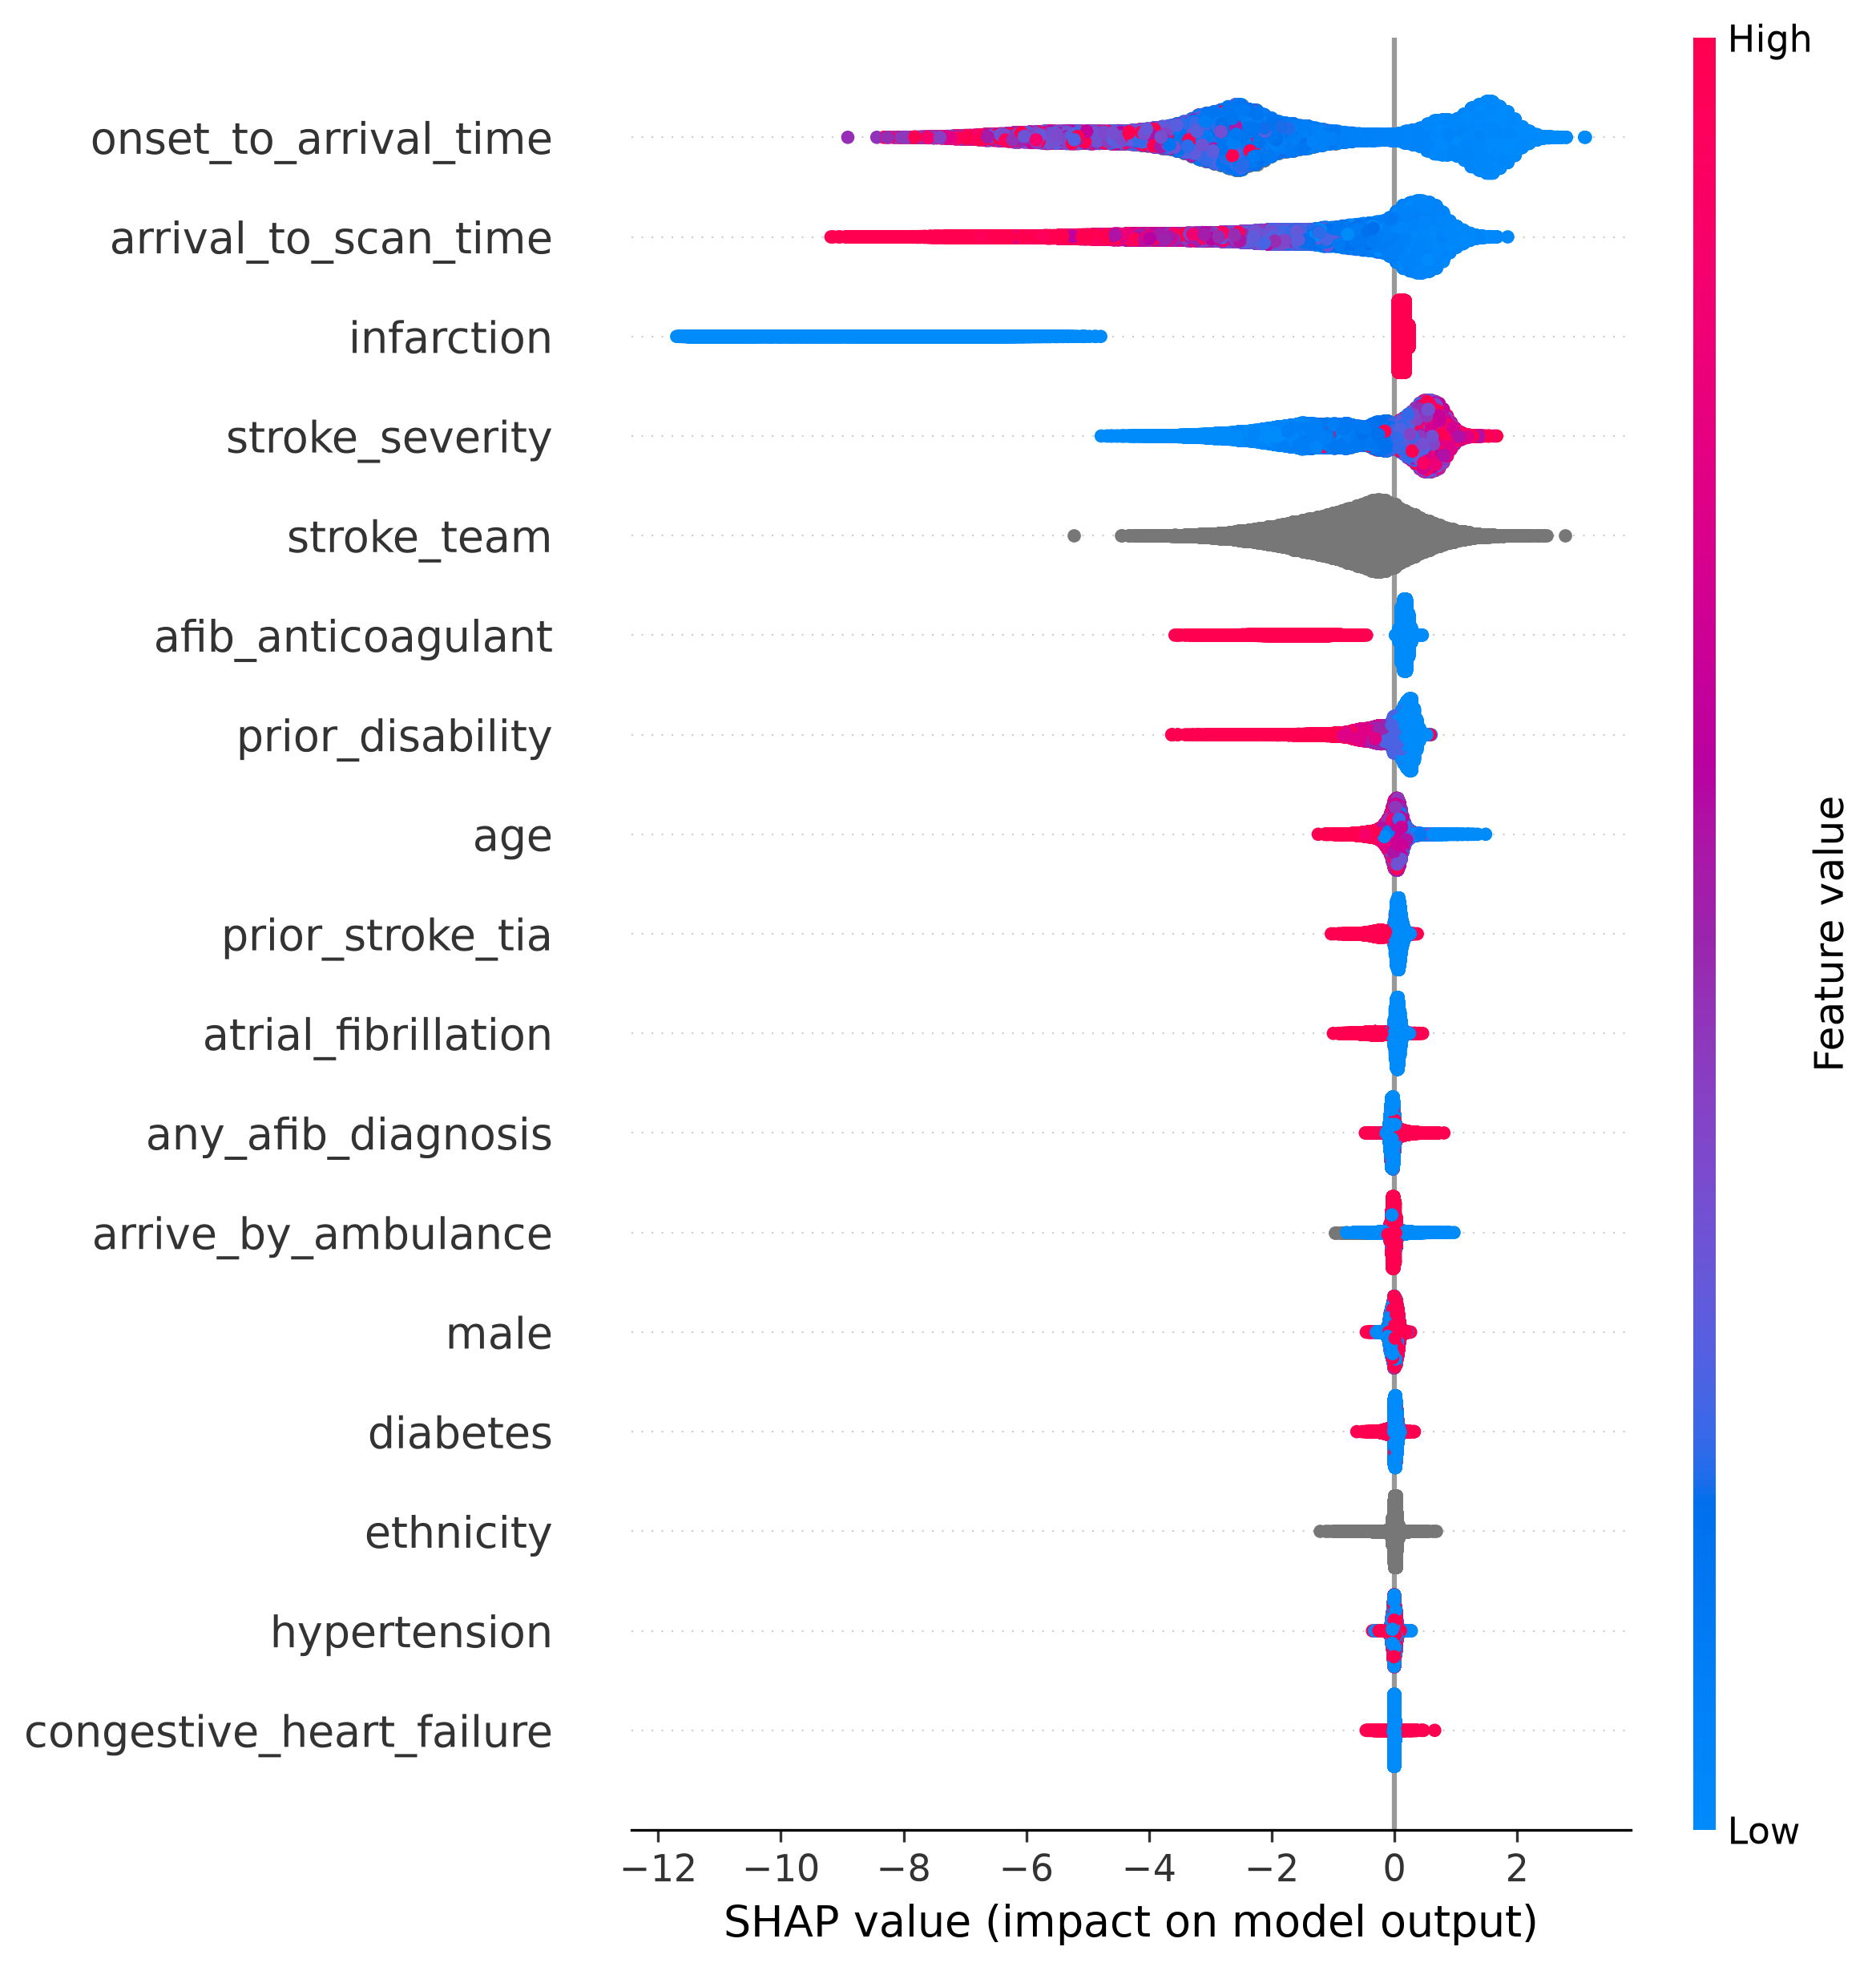
\includegraphics[width=\linewidth]{images/shap/shap_all_patients_thrombolysis_use.png}
        %\caption{}
    \end{subfigure}

    \vspace{0.5cm} % Optional vertical space between rows

    % Bottom left image (~45% width)
    \begin{subfigure}{0.407\textwidth}
        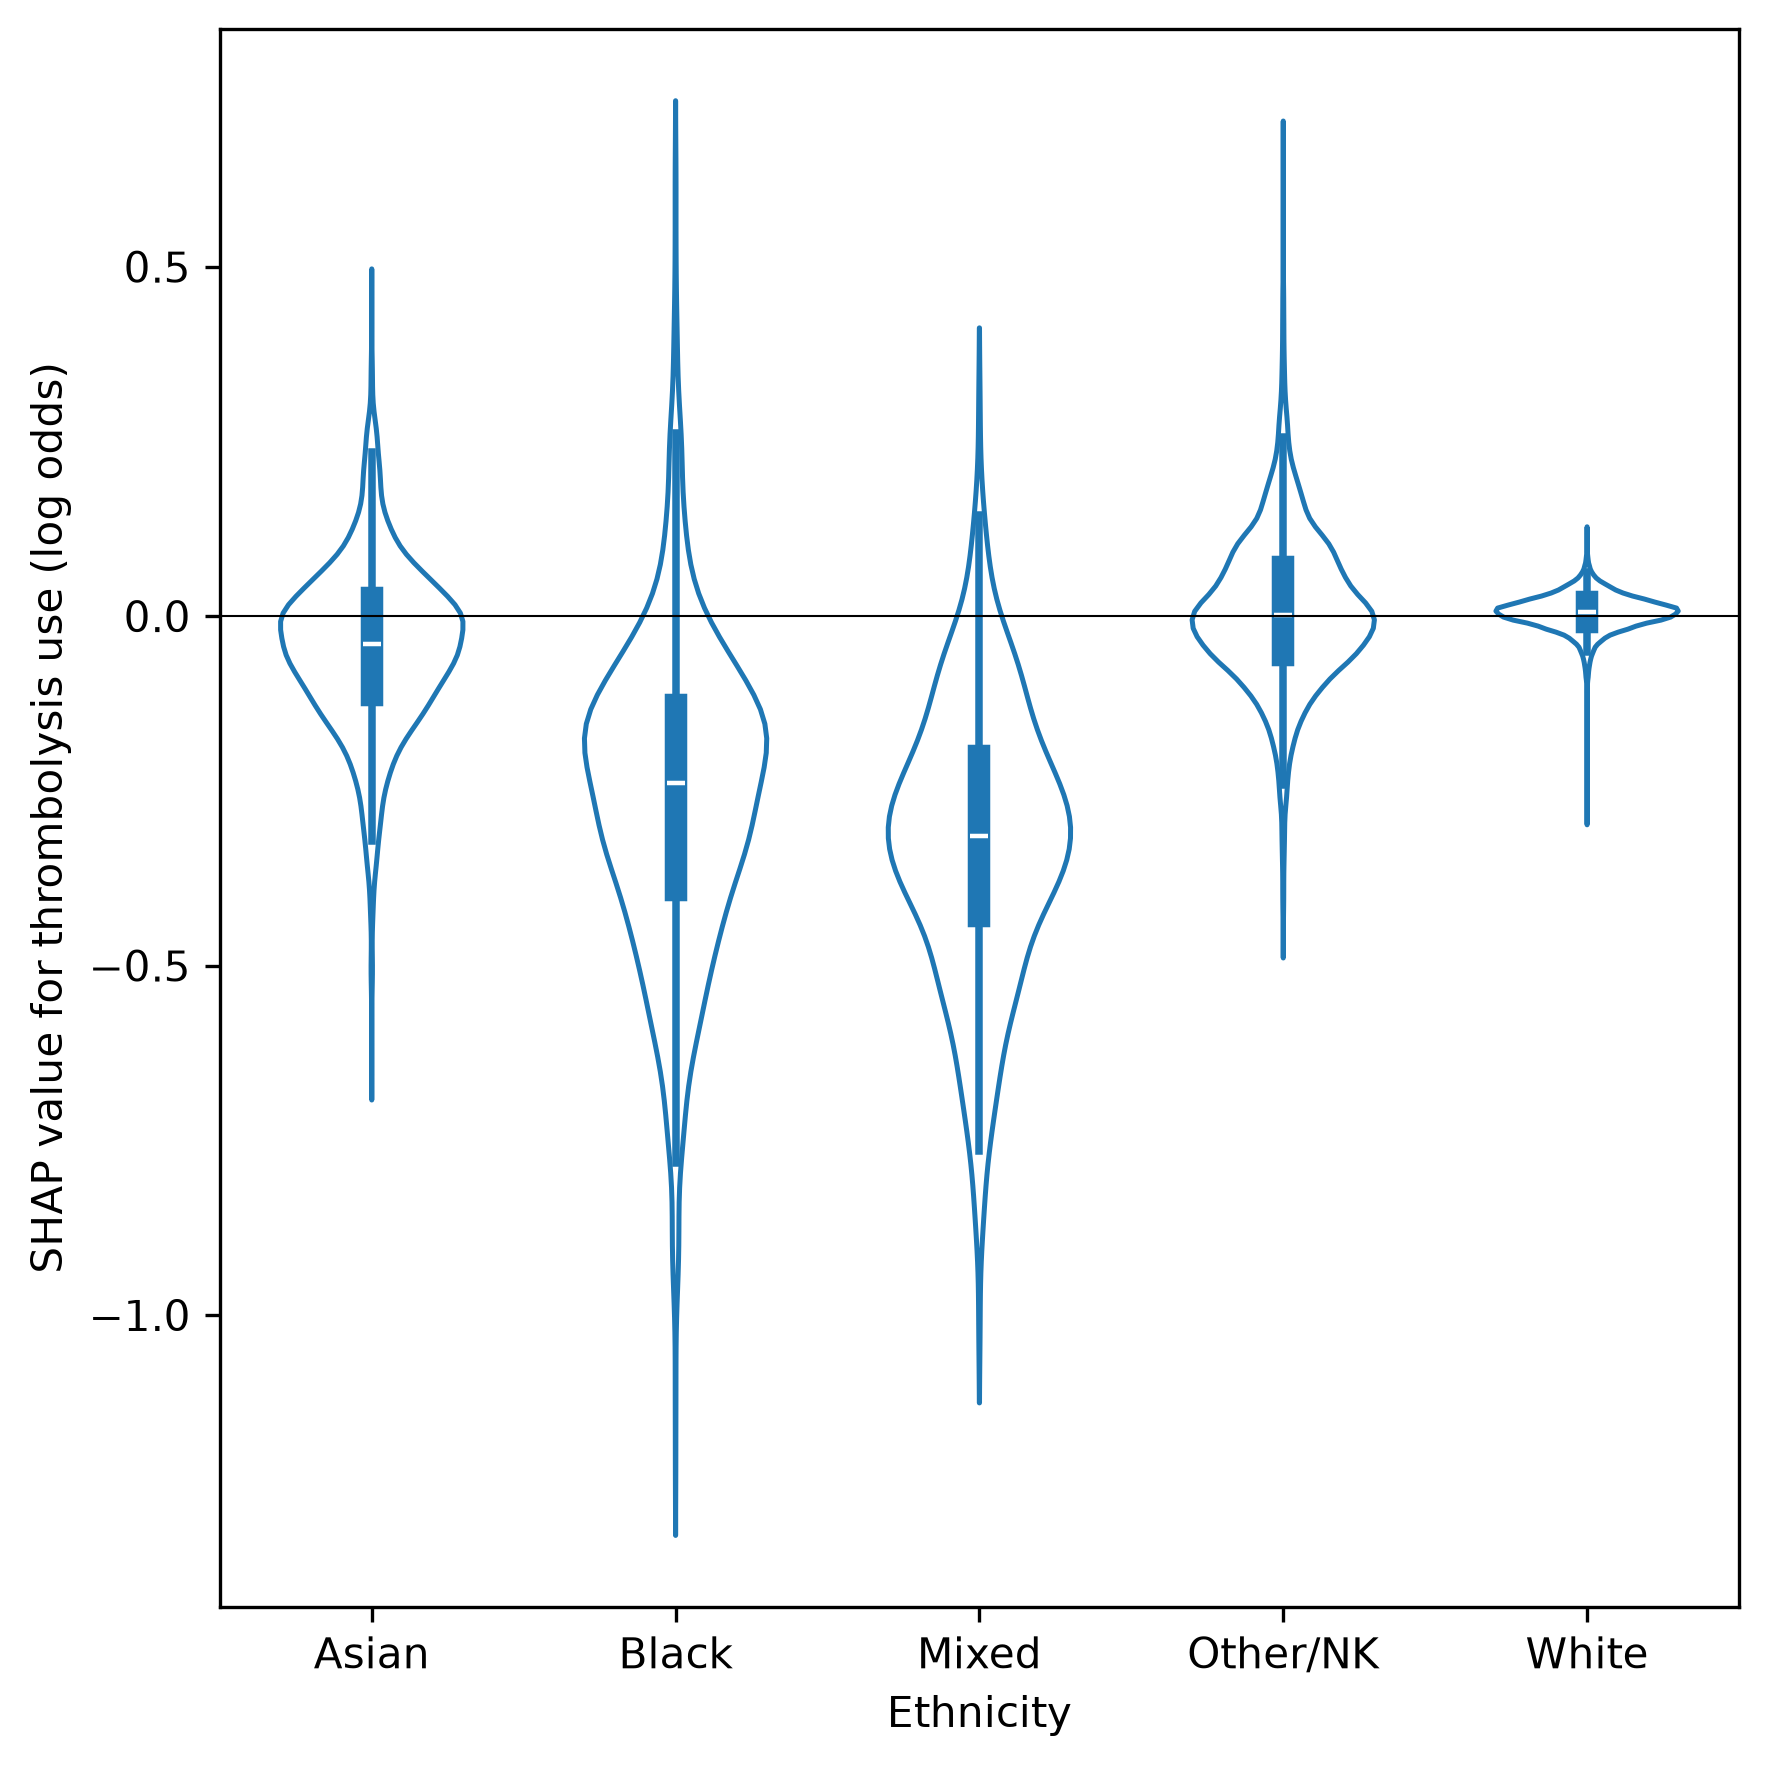
\includegraphics[width=\linewidth]{images/shap/shap_all_patients_thrombolysis_use_ethnicity.png}
        %\caption{}
    \end{subfigure}
    \hfill % Adds flexible horizontal spacing
    % Bottom right image (~55% width)
    \begin{subfigure}{0.543\textwidth}
        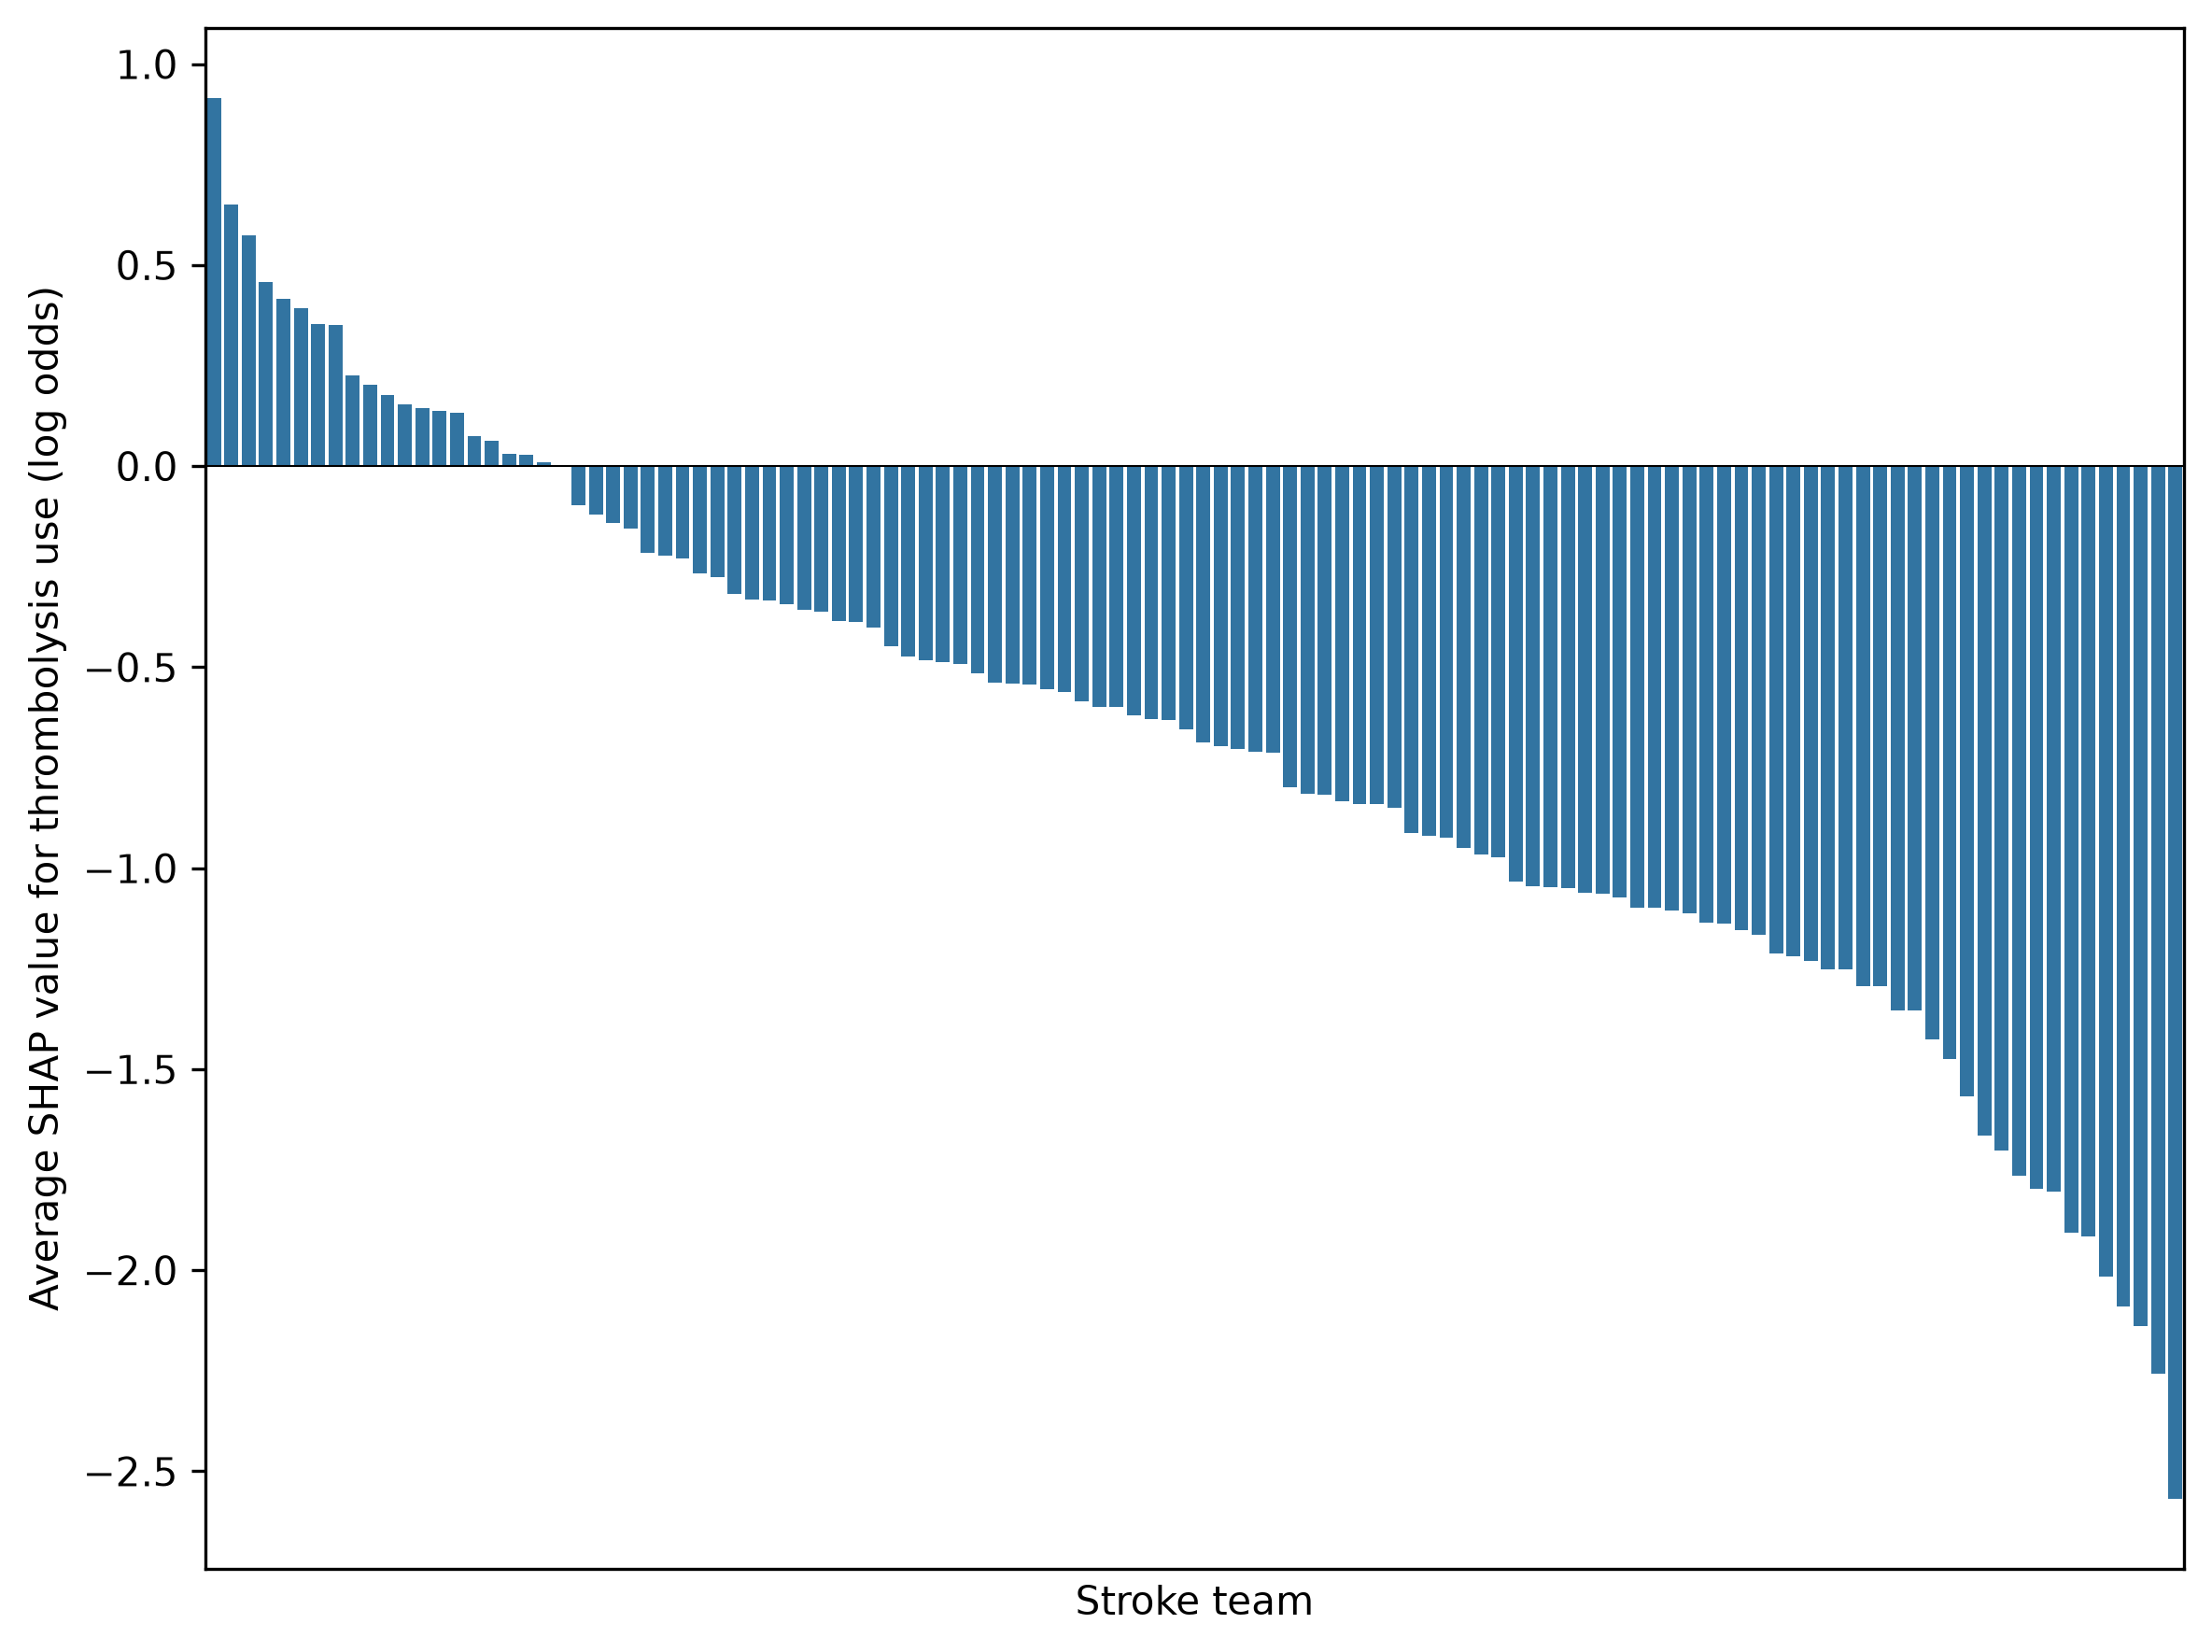
\includegraphics[width=\linewidth]{images/shap/shap_all_patients_thrombolysis_use_stroke_team.png}
        %\caption{}
    \end{subfigure}

    \caption{SHAP analysis of feature contributions to predicting use of thrombolysis in stroke patients. \textit{Top}: A SHAP summary plot detailing the impact of features on the model's log-odds predictions. Each point represents an individual patient instance. The position on the x-axis indicates the SHAP value, where positive values increase the predicted odds of receiving thrombolysis, and negative values decrease it. For continuous and binary variables, colour represents the original feature value (red indicating high values; blue indicating low values). Categorical variables (\textit{stroke team} and \textit{ethnicity}) are plotted in grey. \textit{Bottom left}: Violin plots illustrating the distribution of SHAP values across distinct ethnic groups. This panel highlights the marginal impact and variance of ethnicity on the model's prediction for thrombolysis use. \textit{Bottom Right}: A ranked bar chart displaying the average SHAP value associated with each individual stroke team. This panel visualizes institutional variation, reflecting the contribution of the treating stroke team to the predicted likelihood of receiving thrombolysis after accounting for patient-level clinical characteristics.}  
    \label{fig:shap_thrombolysis_all}
\end{figure}


%%%%%%%%%%%%%%%%%%%% Use of thrombectomy %%%%%%%%%%%%%%%%%%%%%%%%

\begin{figure}[htbp]
    \centering
    
    % Top image (Full width)
    \begin{subfigure}{0.50\textwidth}
        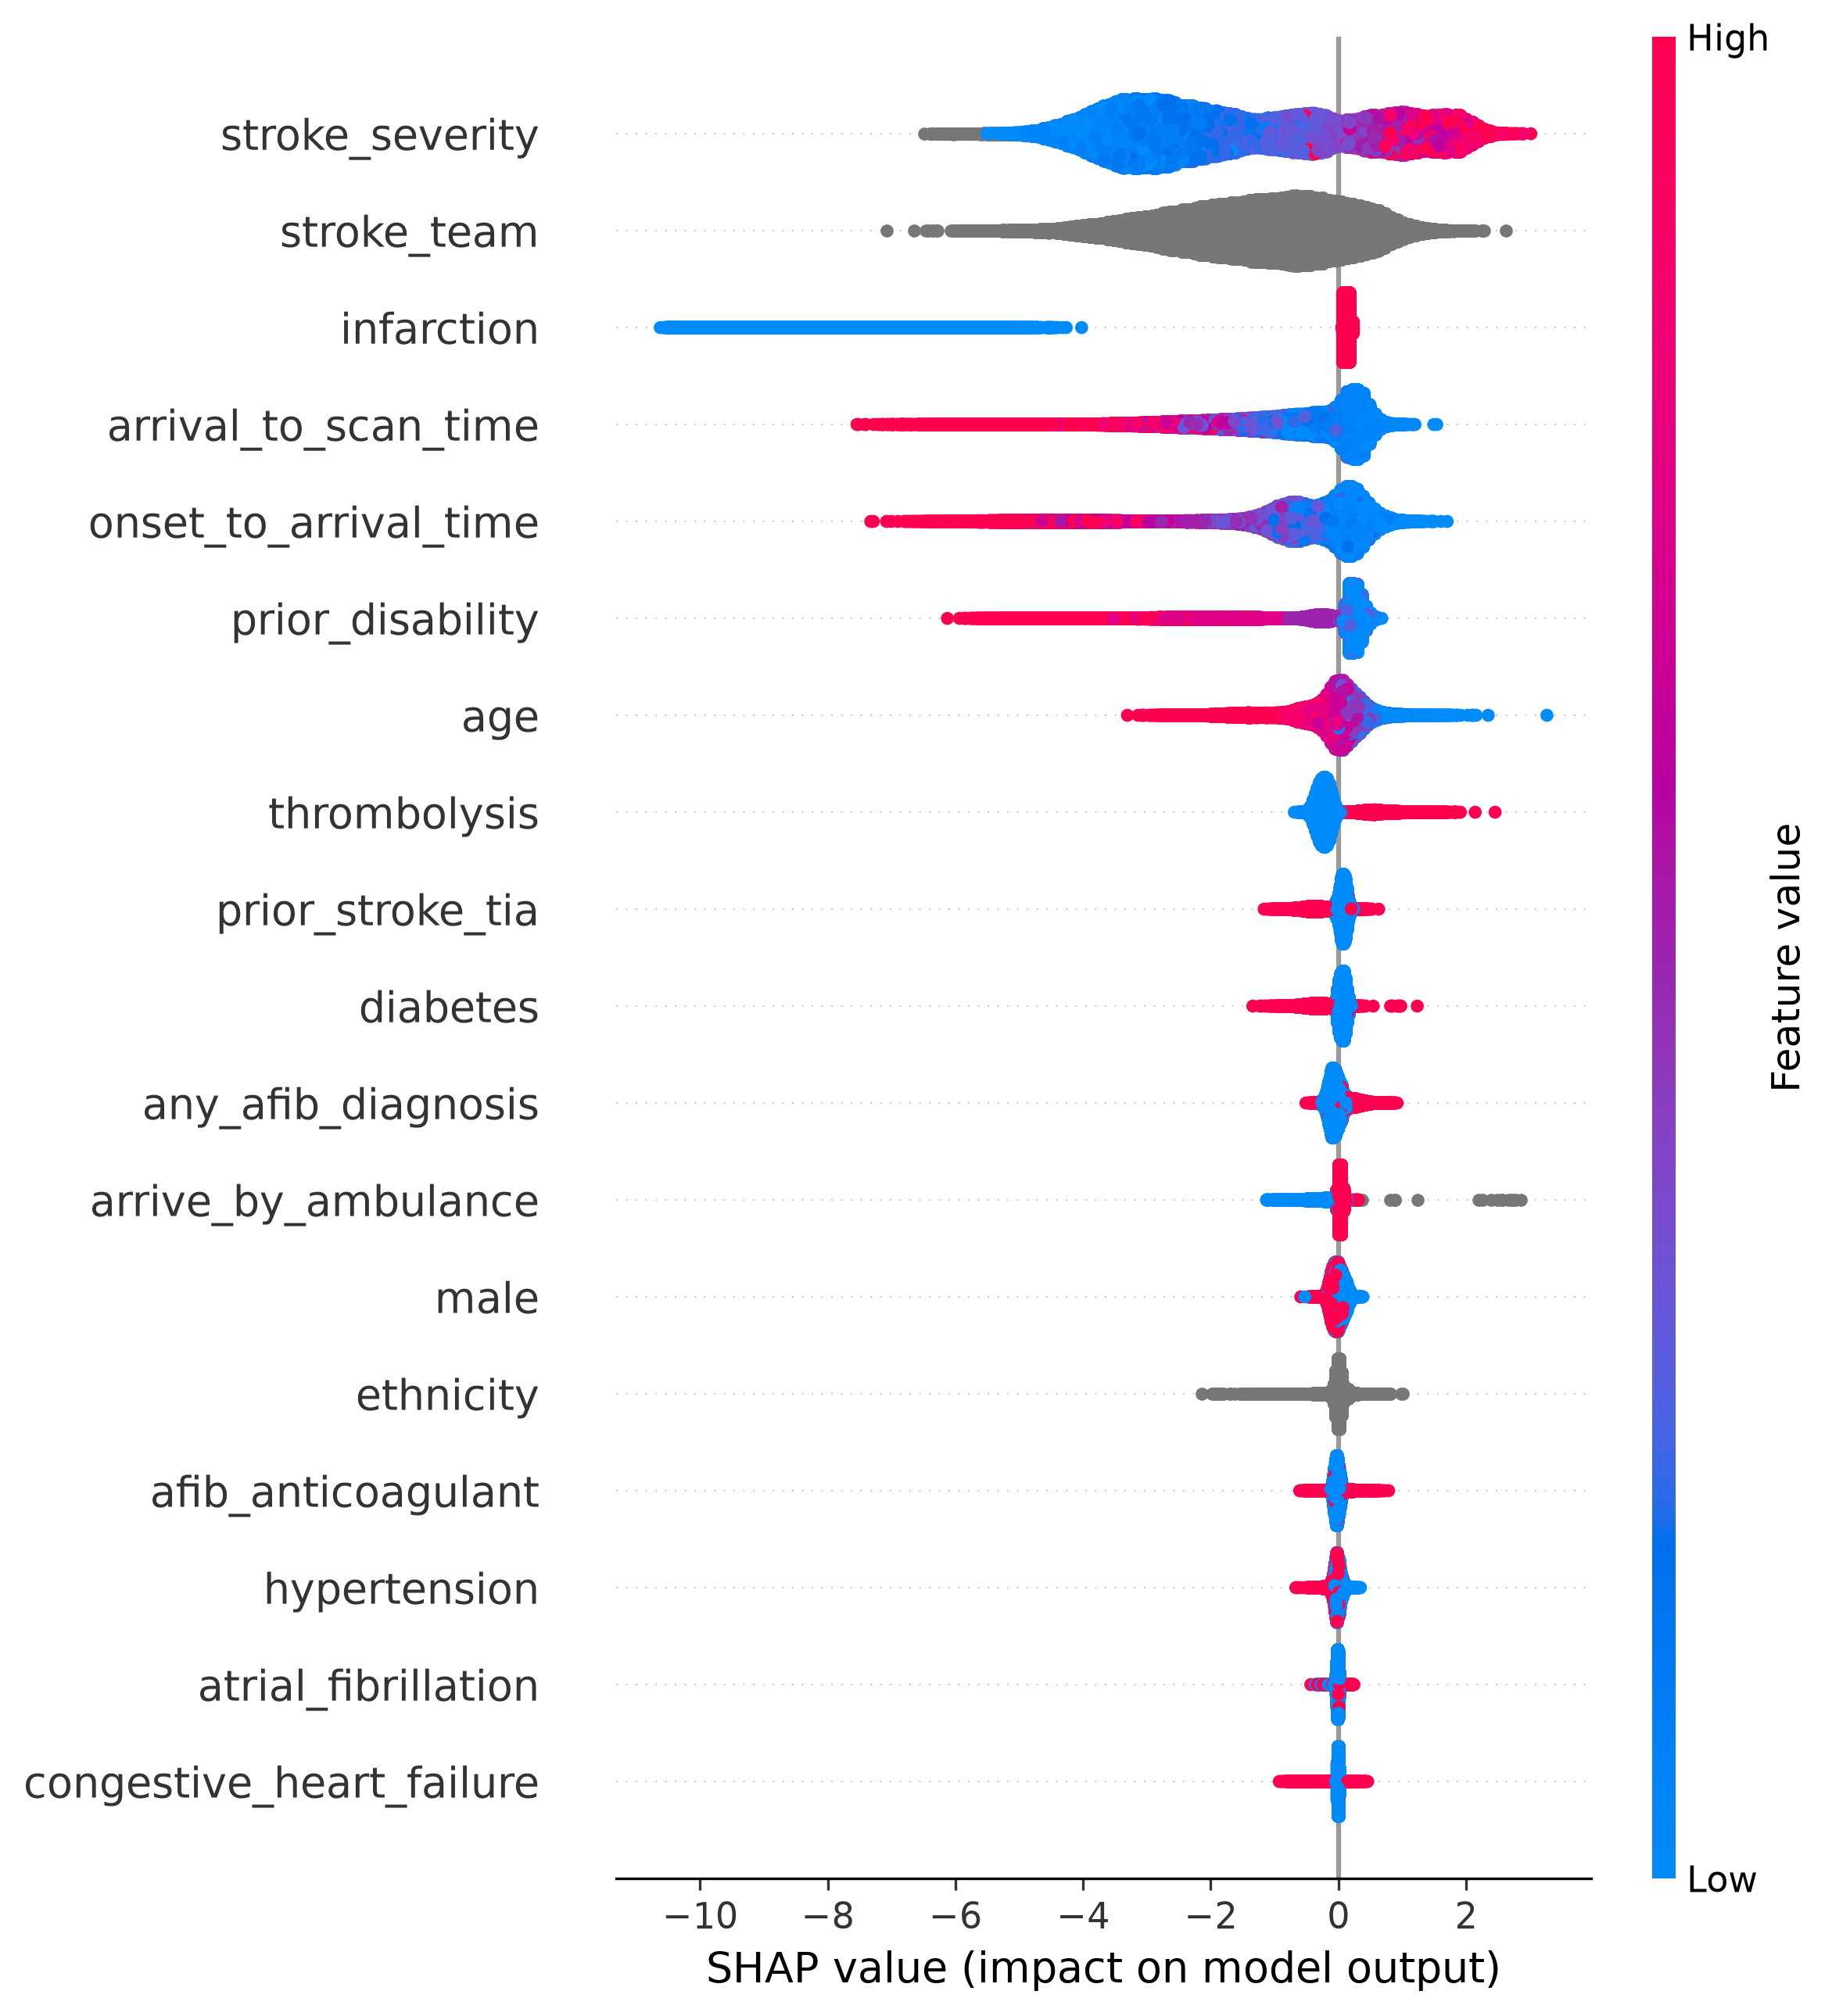
\includegraphics[width=\linewidth]{images/shap/shap_all_patients_thrombectomy_use.png}
        %\caption{}
    \end{subfigure}

    \vspace{0.5cm} % Optional vertical space between rows

    % Bottom left image (~45% width)
    \begin{subfigure}{0.407\textwidth}
        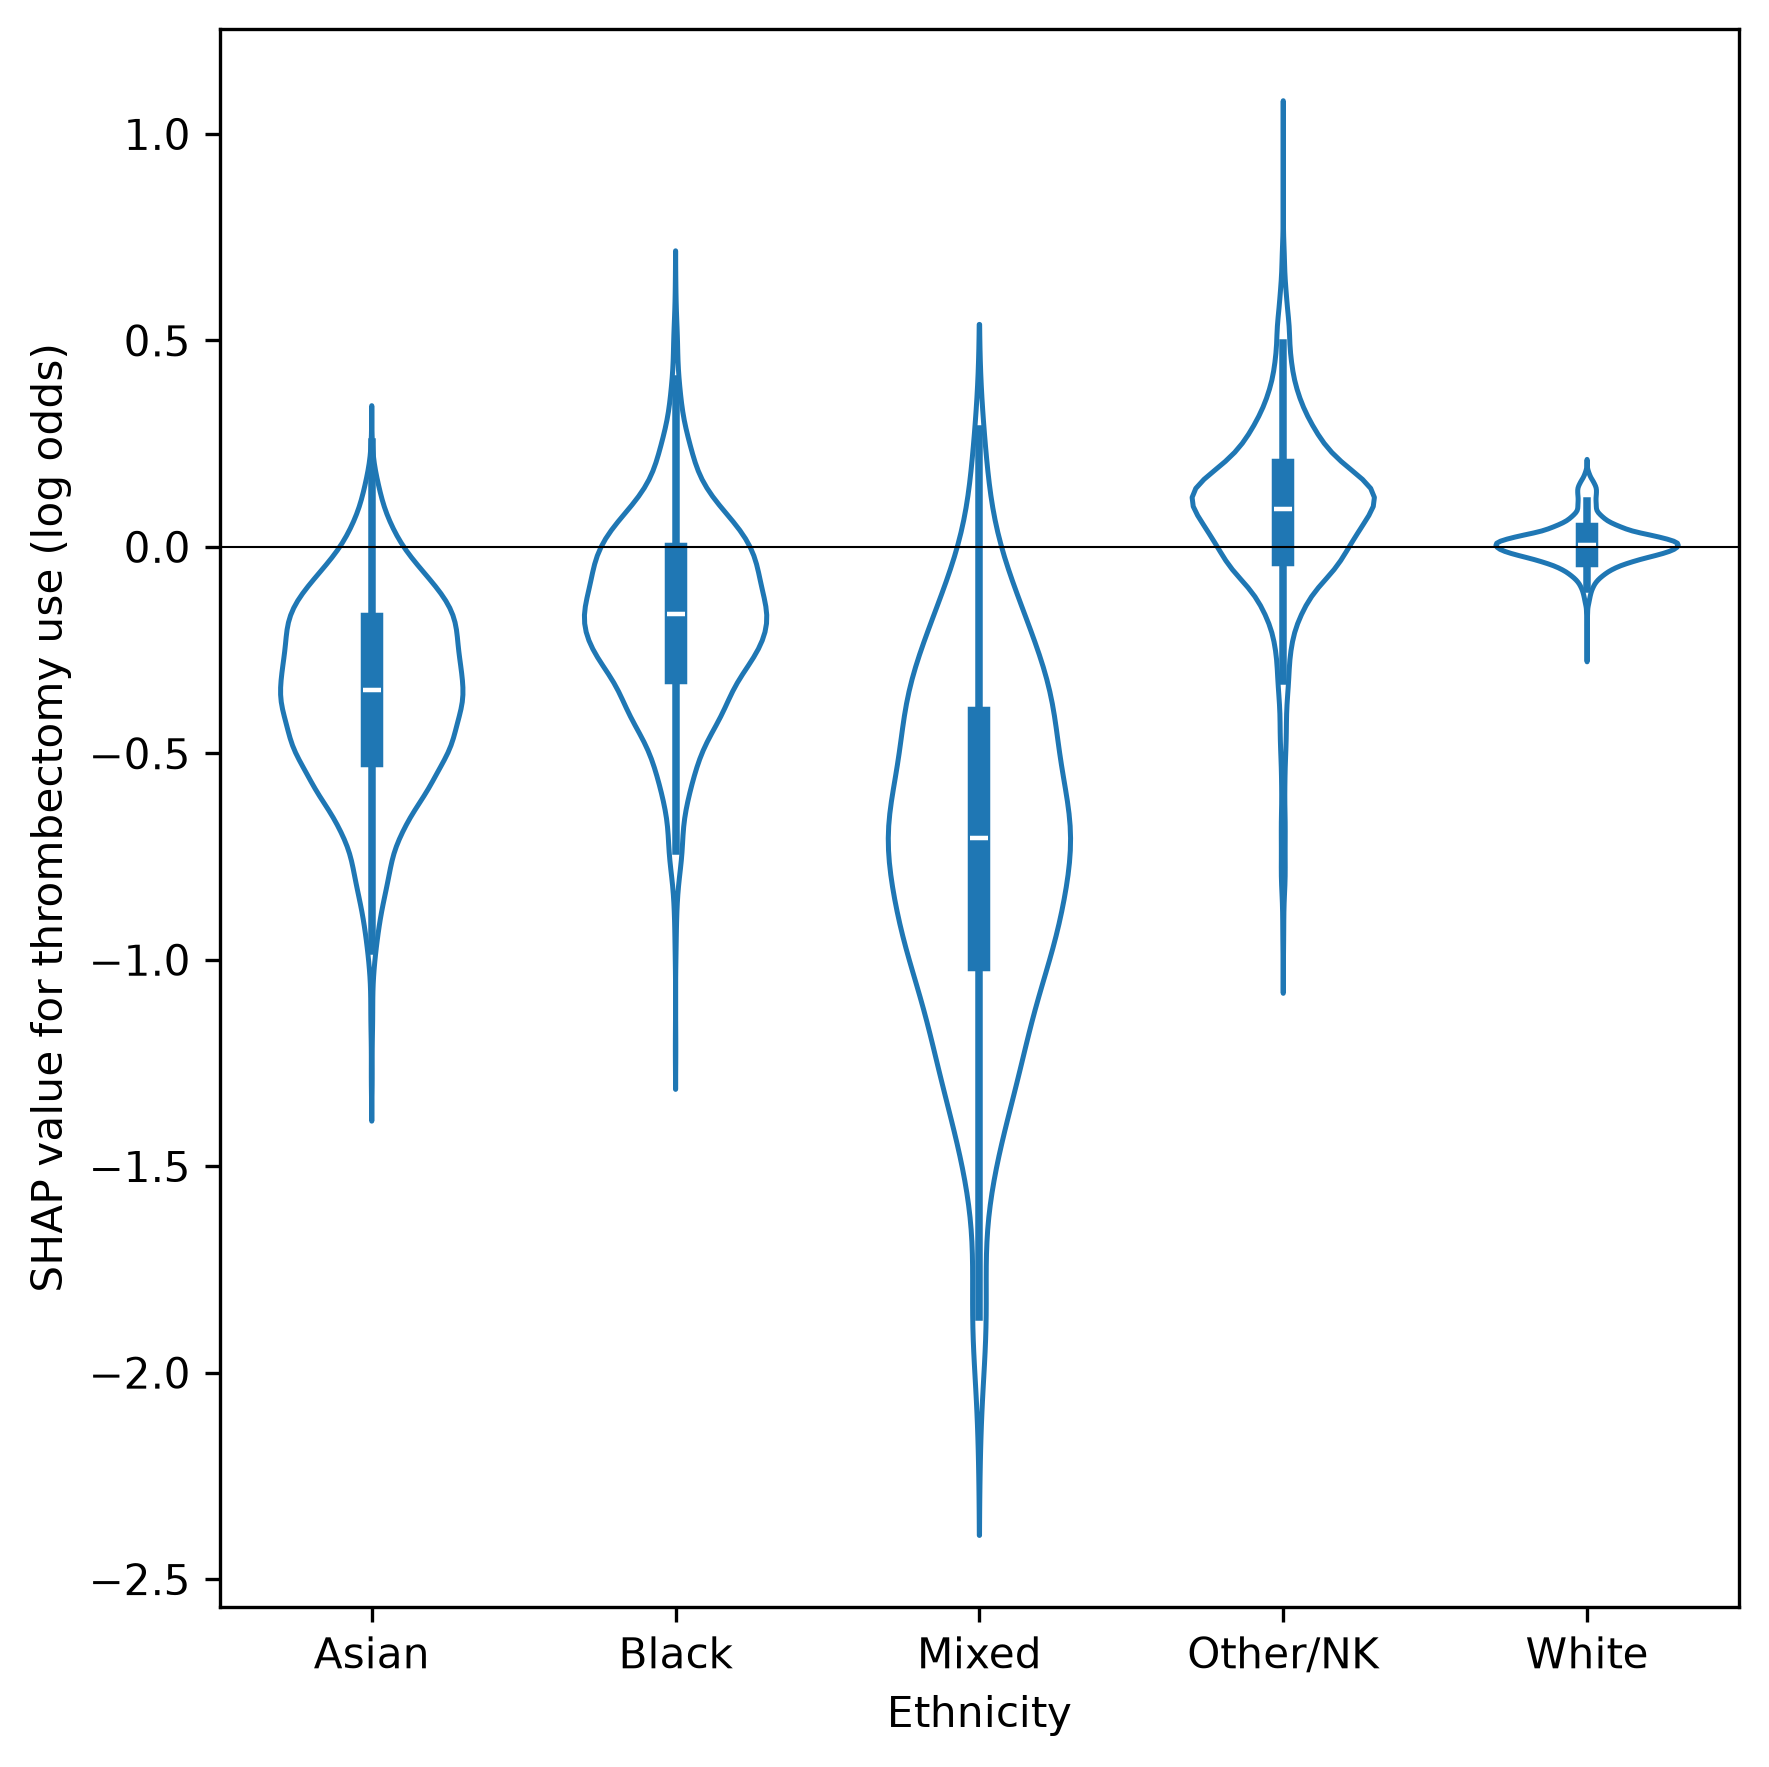
\includegraphics[width=\linewidth]{images/shap/shap_all_patients_thrombectomy_use_ethnicity.png}
        %\caption{}
    \end{subfigure}
    \hfill % Adds flexible horizontal spacing
    % Bottom right image (~55% width)
    \begin{subfigure}{0.543\textwidth}
        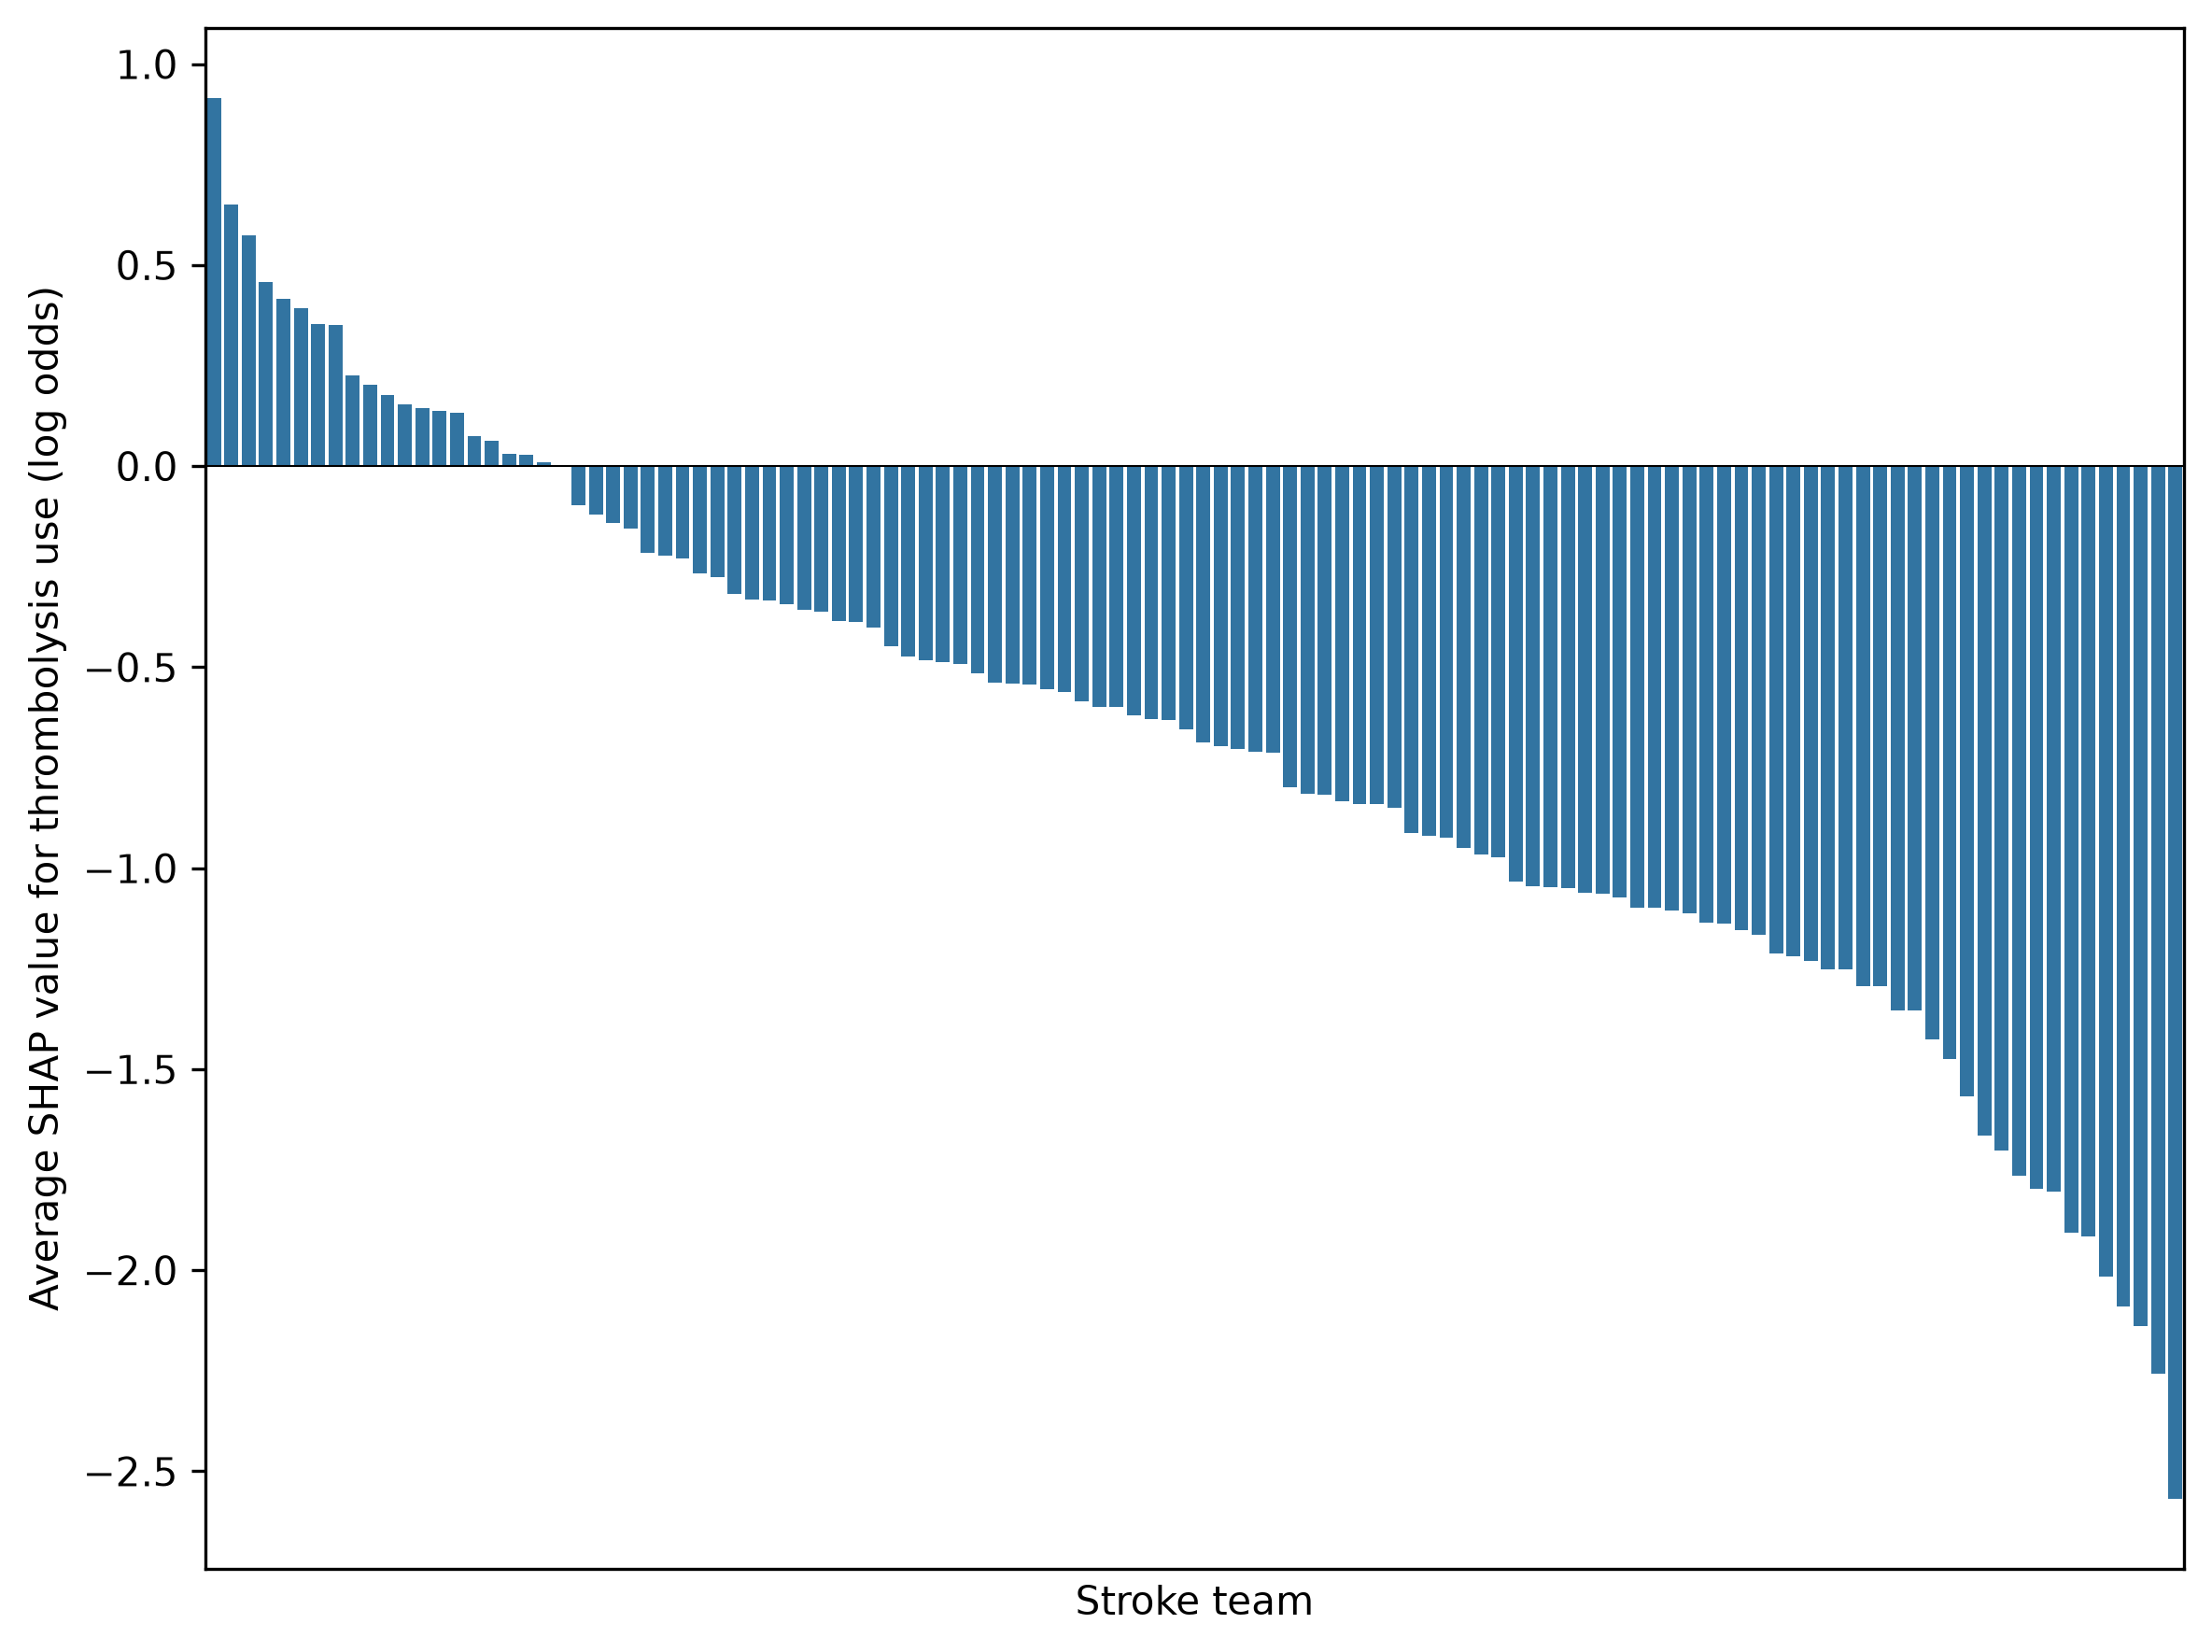
\includegraphics[width=\linewidth]{images/shap/shap_all_patients_thrombolysis_use_stroke_team.png}
        %\caption{}
    \end{subfigure}

    \caption{SHAP analysis of feature contributions to predicting use of thrombectomy in stroke patients. \textit{Top}: A SHAP summary plot detailing the impact of features on the model's log-odds predictions. Each point represents an individual patient instance. The position on the x-axis indicates the SHAP value, where positive values increase the predicted odds of receiving thrombectomy, and negative values decrease it. For continuous and binary variables, colour represents the original feature value (red indicating high values; blue indicating low values). Categorical variables (\textit{stroke team} and \textit{ethnicity}) are plotted in grey. \textit{Bottom left}: Violin plots illustrating the distribution of SHAP values across distinct ethnic groups. This panel highlights the marginal impact and variance of ethnicity on the model's prediction for thrombectomy use. \textit{Bottom Right}: A ranked bar chart displaying the average SHAP value associated with each individual stroke team. This panel visualizes institutional variation, reflecting the contribution of the treating stroke team to the predicted likelihood of receiving thrombectomy after accounting for patient-level clinical characteristics.}  
    \label{fig:shap_thrombectomy_all}
\end{figure}


%%%%%%%%%%%%%%%%%%%% Thrombolysis-induced haemorrhage %%%%%%%%%%%%%%%%%%%%%%%%

\begin{figure}[htbp]
    \centering
    
    % Top image (Full width)
    \begin{subfigure}{0.50\textwidth}
        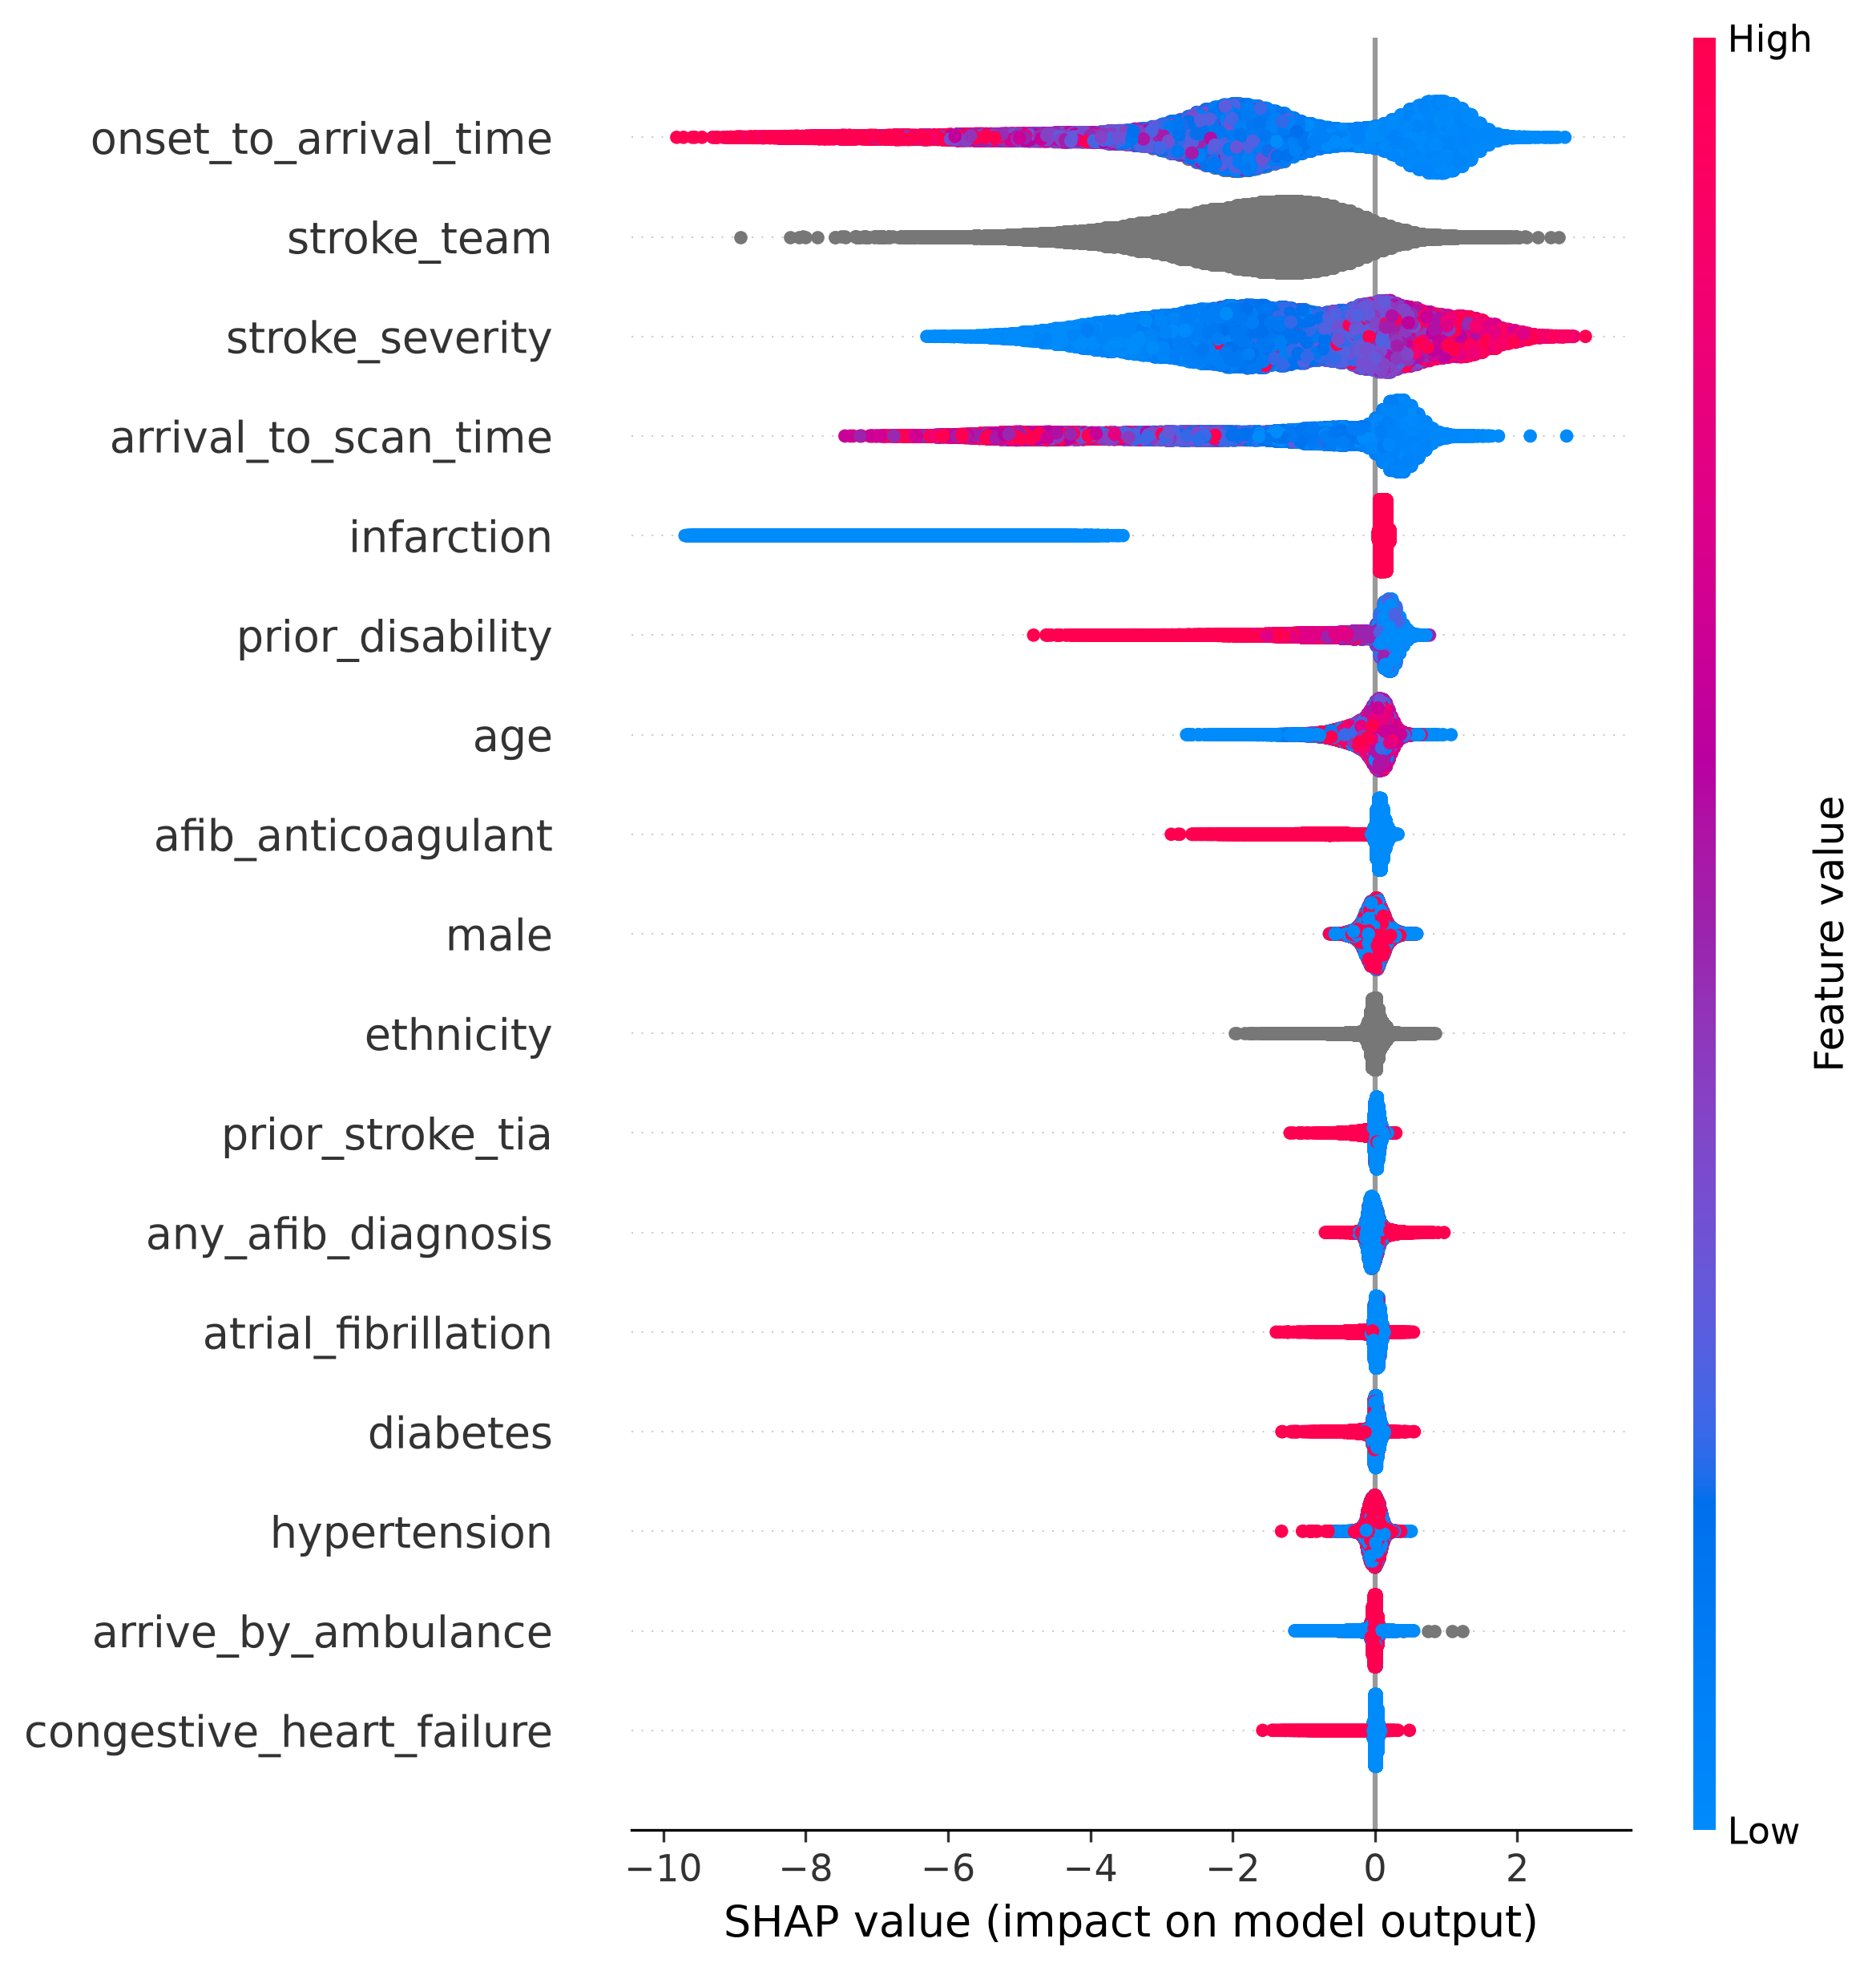
\includegraphics[width=\linewidth]{images/shap/shap_thrombolysis_induced_haemorrhage_use.png}
        %\caption{}
    \end{subfigure}

    \vspace{0.5cm} % Optional vertical space between rows

    % Bottom left image (~45% width)
    \begin{subfigure}{0.407\textwidth}
        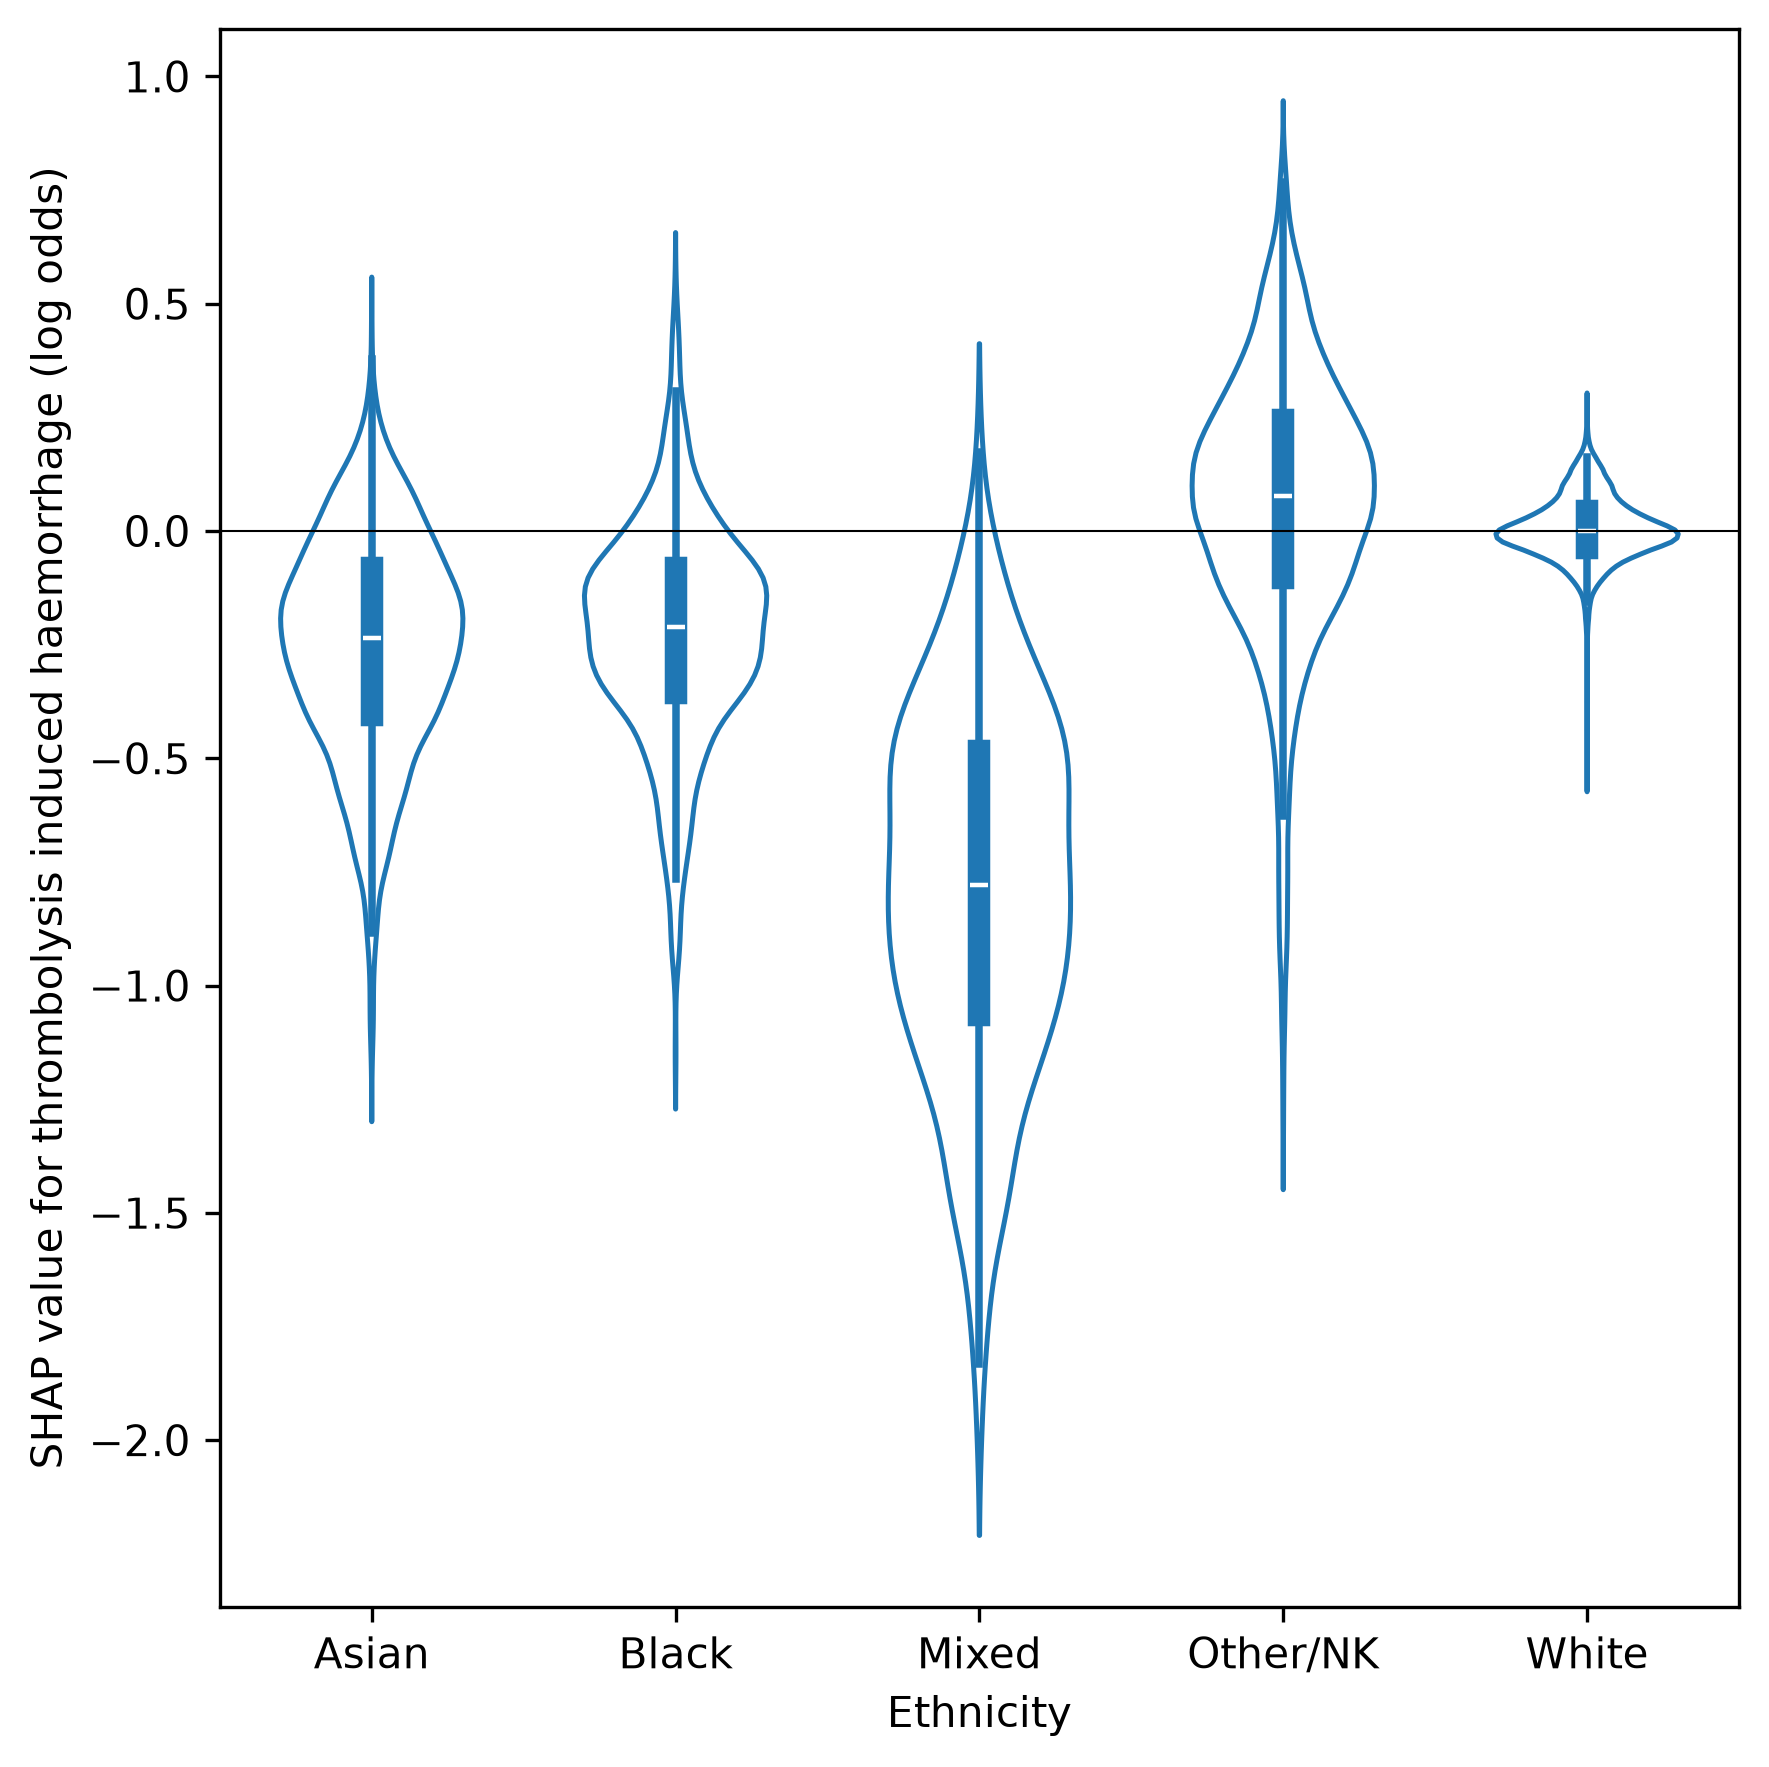
\includegraphics[width=\linewidth]{images/shap/shap_thrombolysis_induced_haemorrhage_use_ethnicity.png}
        %\caption{}
    \end{subfigure}
    \hfill % Adds flexible horizontal spacing
    % Bottom right image (~55% width)
    \begin{subfigure}{0.543\textwidth}
        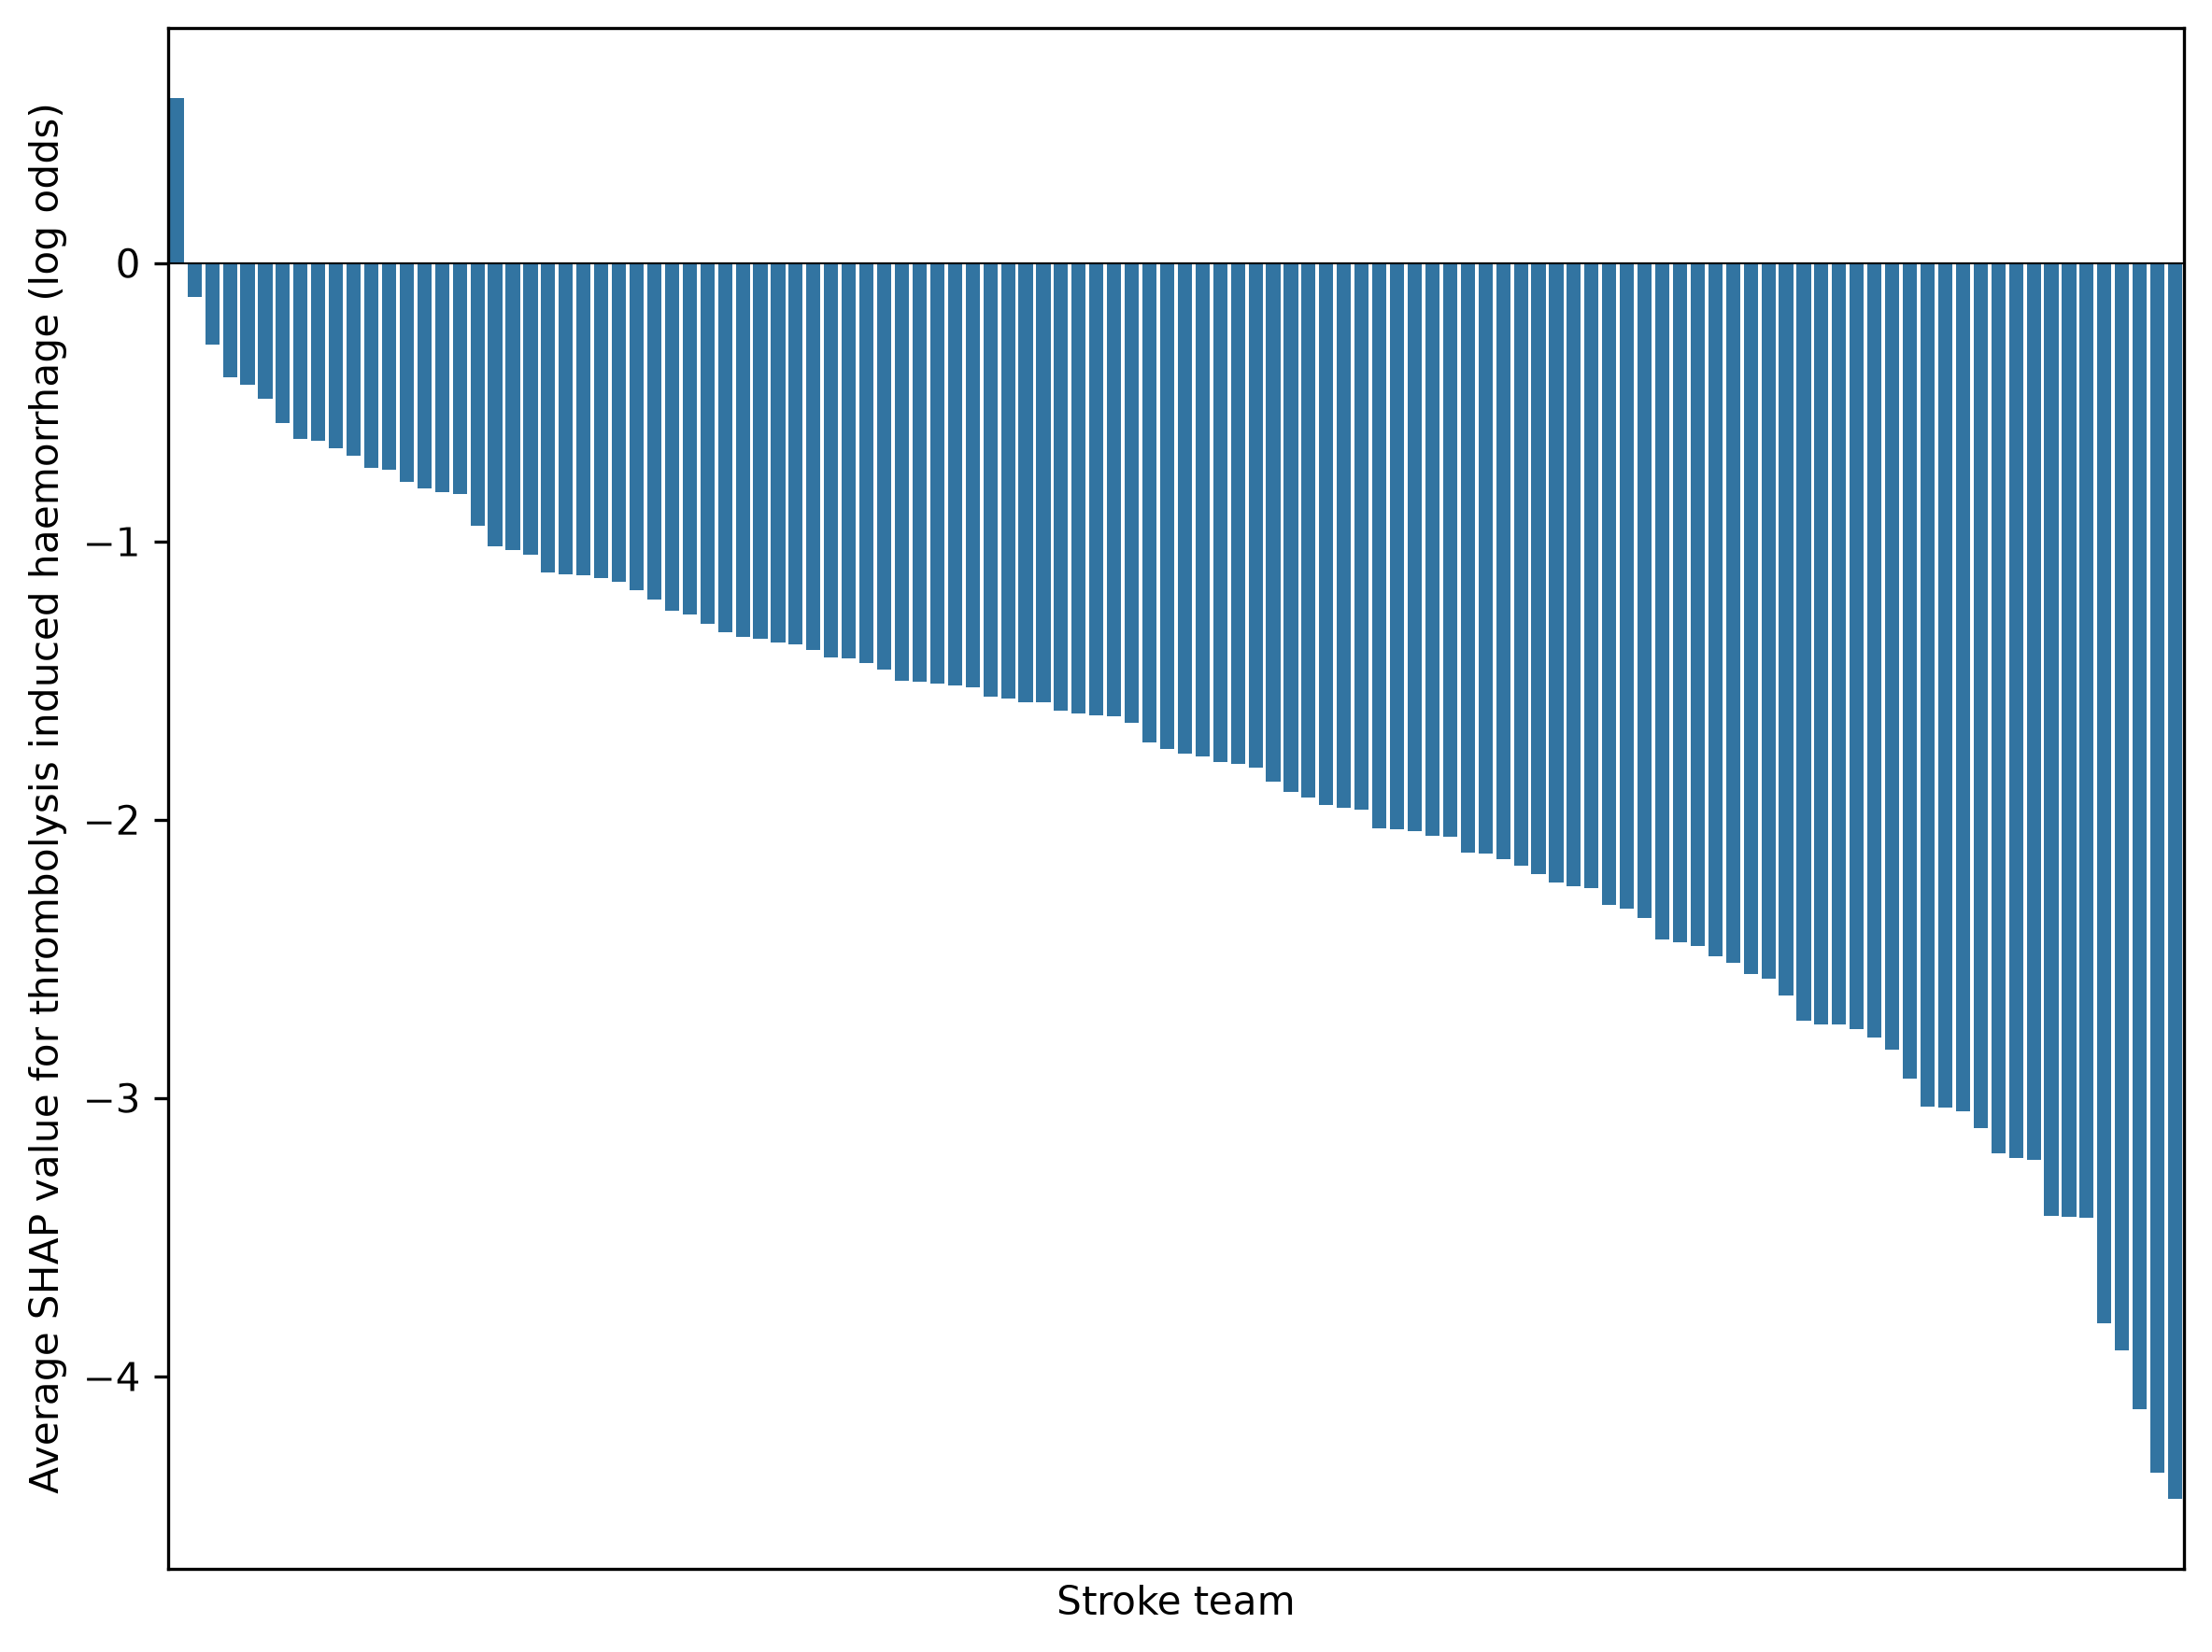
\includegraphics[width=\linewidth]{images/shap/shap_thrombolysis_induced_haemorrhage_use_stroke_team.png}
        %\caption{}
    \end{subfigure}
    \caption{SHAP analysis of feature contributions to predicting thrombolysis-induced haemorrhage in stroke patients who have received thrombolysis. \textit{Top}: A SHAP summary plot detailing the impact of features on the model's log-odds predictions. Each point represents an individual patient instance. The position on the x-axis indicates the SHAP value, where positive values increase the predicted odds of haemorrhage, and negative values decrease it. For continuous and binary variables, colour represents the original feature value (red indicating high values; blue indicating low values). Categorical variables (\textit{stroke team} and \textit{ethnicity}) are plotted in grey. \textit{Bottom left}: Violin plots illustrating the distribution of SHAP values across distinct ethnic groups. This panel highlights the marginal impact and variance of ethnicity on the model's prediction for haemorrhage risk. \textit{Bottom Right}: A ranked bar chart displaying the average SHAP value associated with each individual stroke team. This panel visualizes institutional variation, reflecting the contribution of the treating stroke team to the predicted risk of thrombolysis-induced haemorrhage after accounting for patient-level clinical characteristics.}
    \label{fig:shap_thrombolysis_haemorrhage}
\end{figure}


% ====================================================================================

\newpage

\section{Treatment effects}

The main paper reports treatment effects for a good outcome at discharge, defined as a discharge mRS of 0--2, or a discharge mRS no worse than the patient's pre-stroke mRS. This section repeats each analysis with the mRS threshold set to each possible value (mRS 0--1, 0--2, 0--3, 0--4 and 0--5, the last being survival to discharge), to show whether the conclusions depend on the threshold chosen. At each threshold, a good outcome is a discharge mRS at or below the threshold, or no worse than the patient's pre-stroke mRS. Treatment groups are as defined in the main paper: thrombolysis and thrombectomy, alone or combined, each given early ($\leq$270 minutes after stroke onset) or late ($>$270 minutes).

\subsection{Target trial emulation}

Figures \ref{fig:target_trial_mrs_1} to \ref{fig:target_trial_mrs_5} show treatment effects estimated by matching-based target trial emulation for each mRS threshold. For each treatment group, every treated patient was matched to an untreated patient with similar characteristics (see main Methods), and outcomes were then compared between the treated patients (red) and their matched controls (blue). The difference between each pair of points is the estimated effect of treatment in those who received it.

The left panel of each figure shows mean discharge mRS, which does not depend on the threshold and is therefore the same in every figure; a lower value indicates less disability. The right panel shows the proportion of patients with a good outcome at the given mRS threshold (discharge mRS at or below the threshold, or no worse than before the stroke), where a higher value indicates a better outcome. Because a separate matched control group was constructed for each treatment group, the untreated (blue) values differ between treatment groups, reflecting the different characteristics of the patients who received each treatment.

\begin{figure}
    \centering
    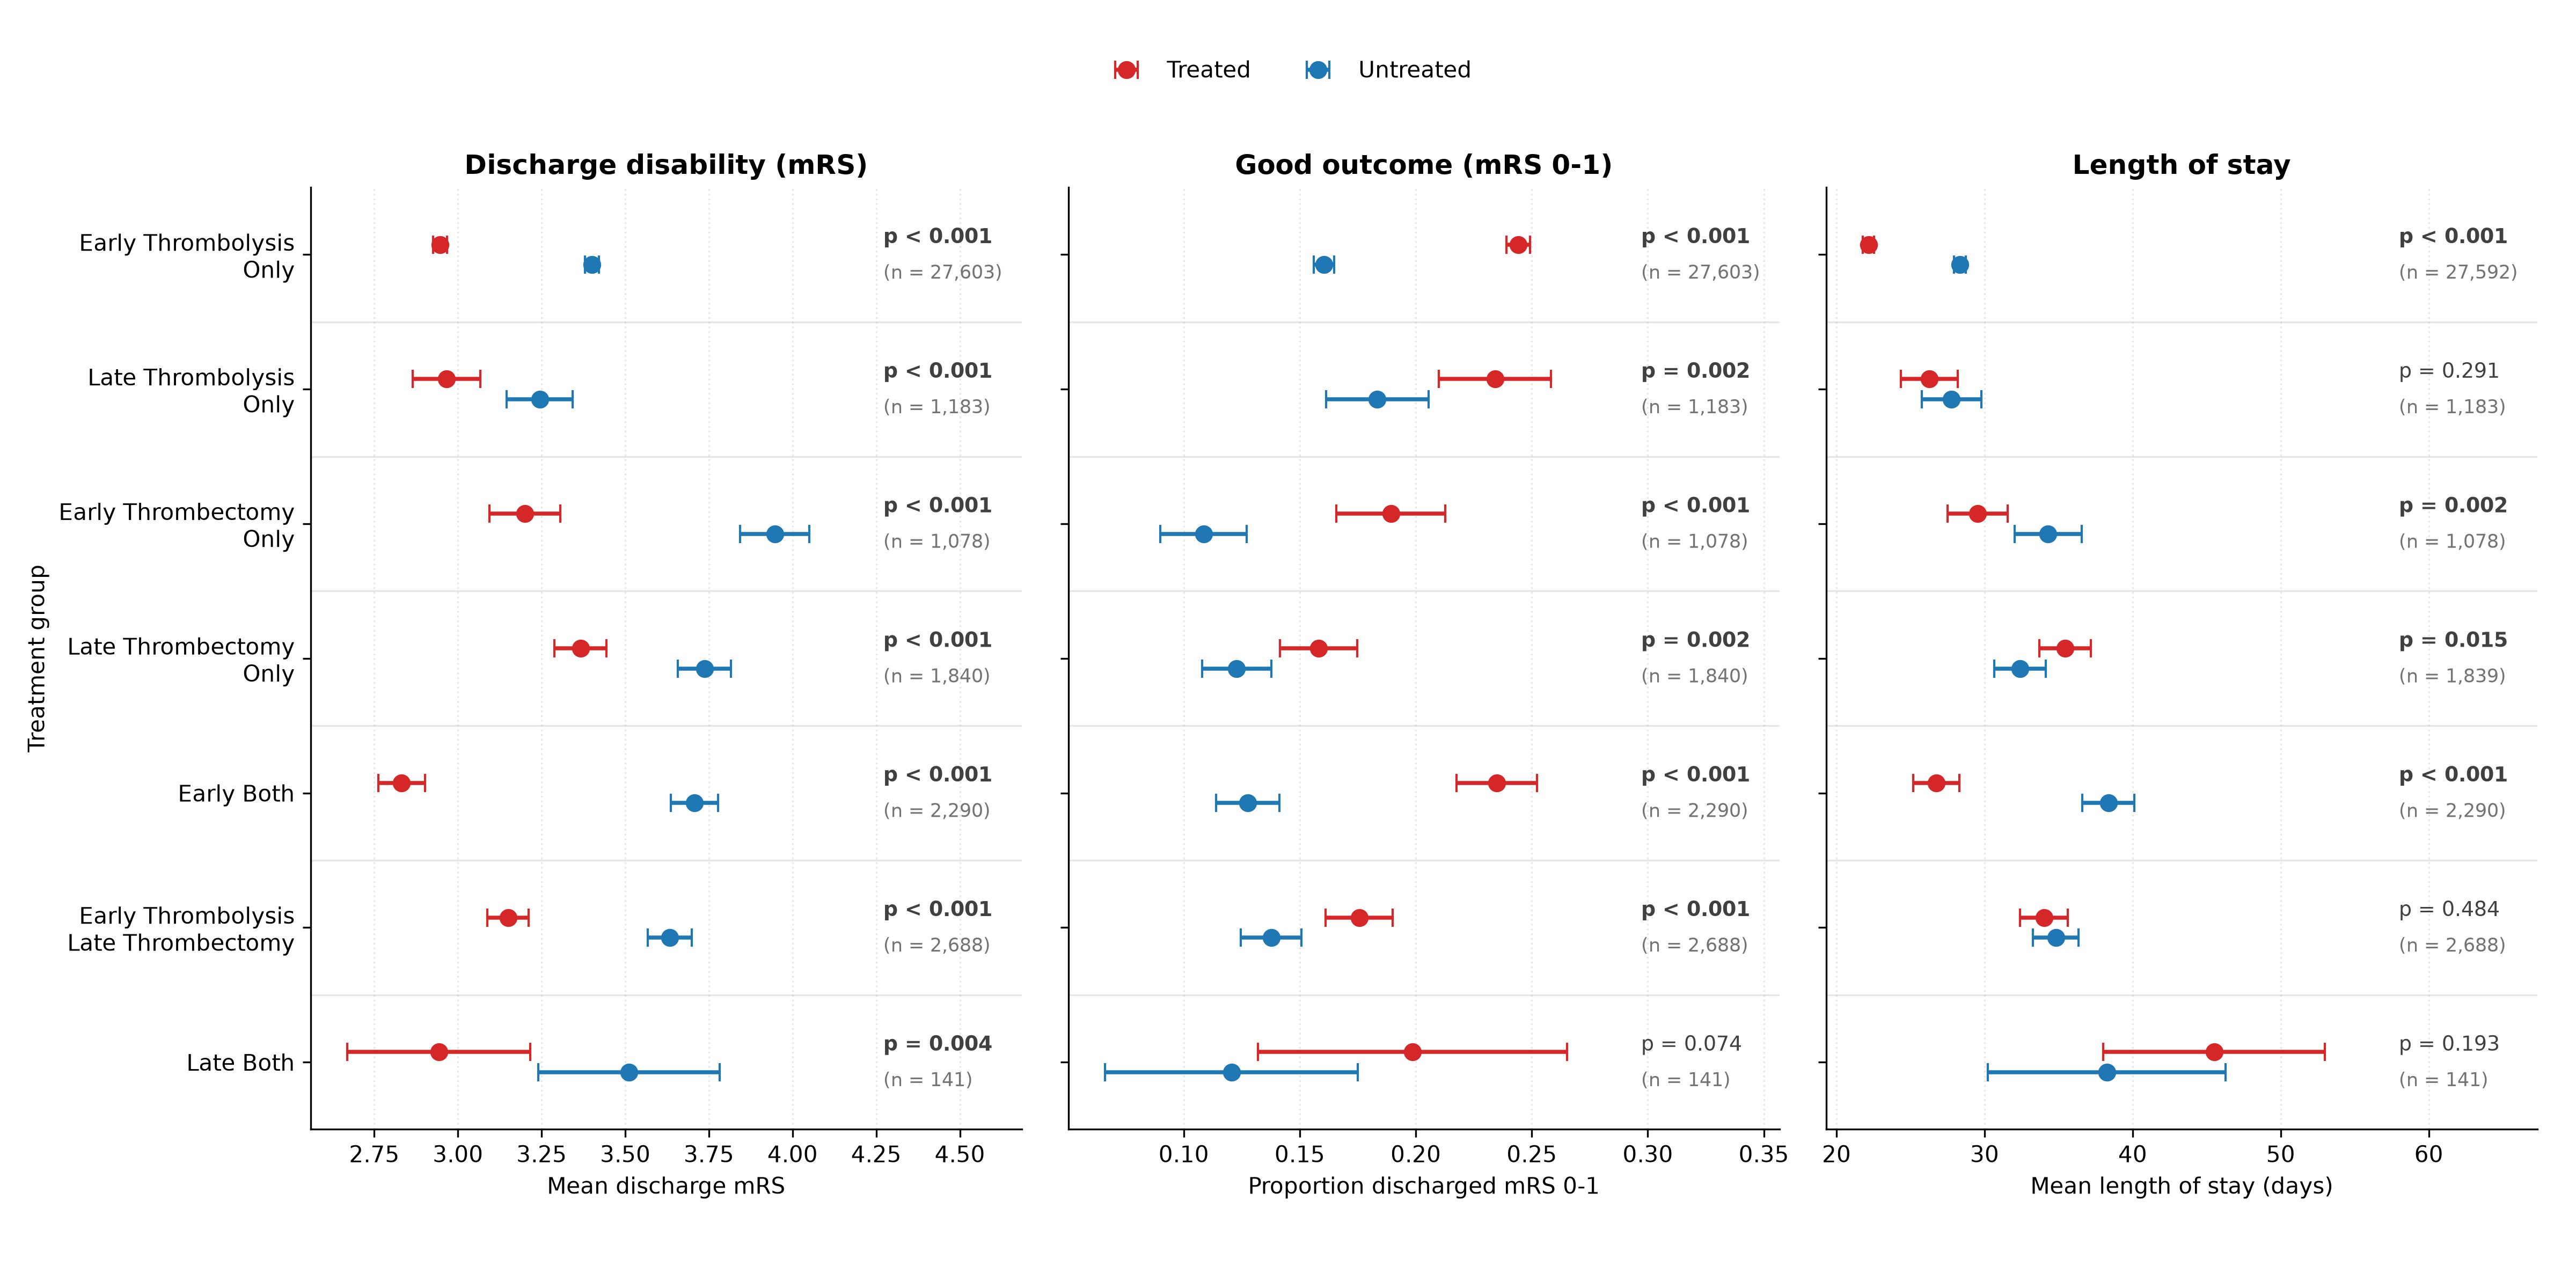
\includegraphics[width=1\linewidth]{images/treatment_effects/target_trial_emulation_mrs_1.png}
    \caption{Target trial emulation of reperfusion-treatment timing strategies and discharge functional outcomes, using matched control and treated patients. Estimated mean discharge modified Rankin Scale (mRS; left panel) and proportion achieving a good outcome at the mRS 0–1 threshold (right panel) are shown for patients receiving each treatment strategy (red) and their emulated untreated comparators (blue). Strategies are defined by early ($\leq$ 270 mins from onset) or late ($>$ 270 mins from onset) intravenous thrombolysis, mechanical thrombectomy, or their combination. Points denote estimated outcomes and horizontal bars 95\% confidence intervals; p-values indicate the treated–untreated comparison within each emulated treatment group, with sample sizes shown. Lower mRS and higher proportions with a good outcome indicate more favourable outcomes.}
    \label{fig:target_trial_mrs_1}
\end{figure}


\begin{figure}
    \centering
    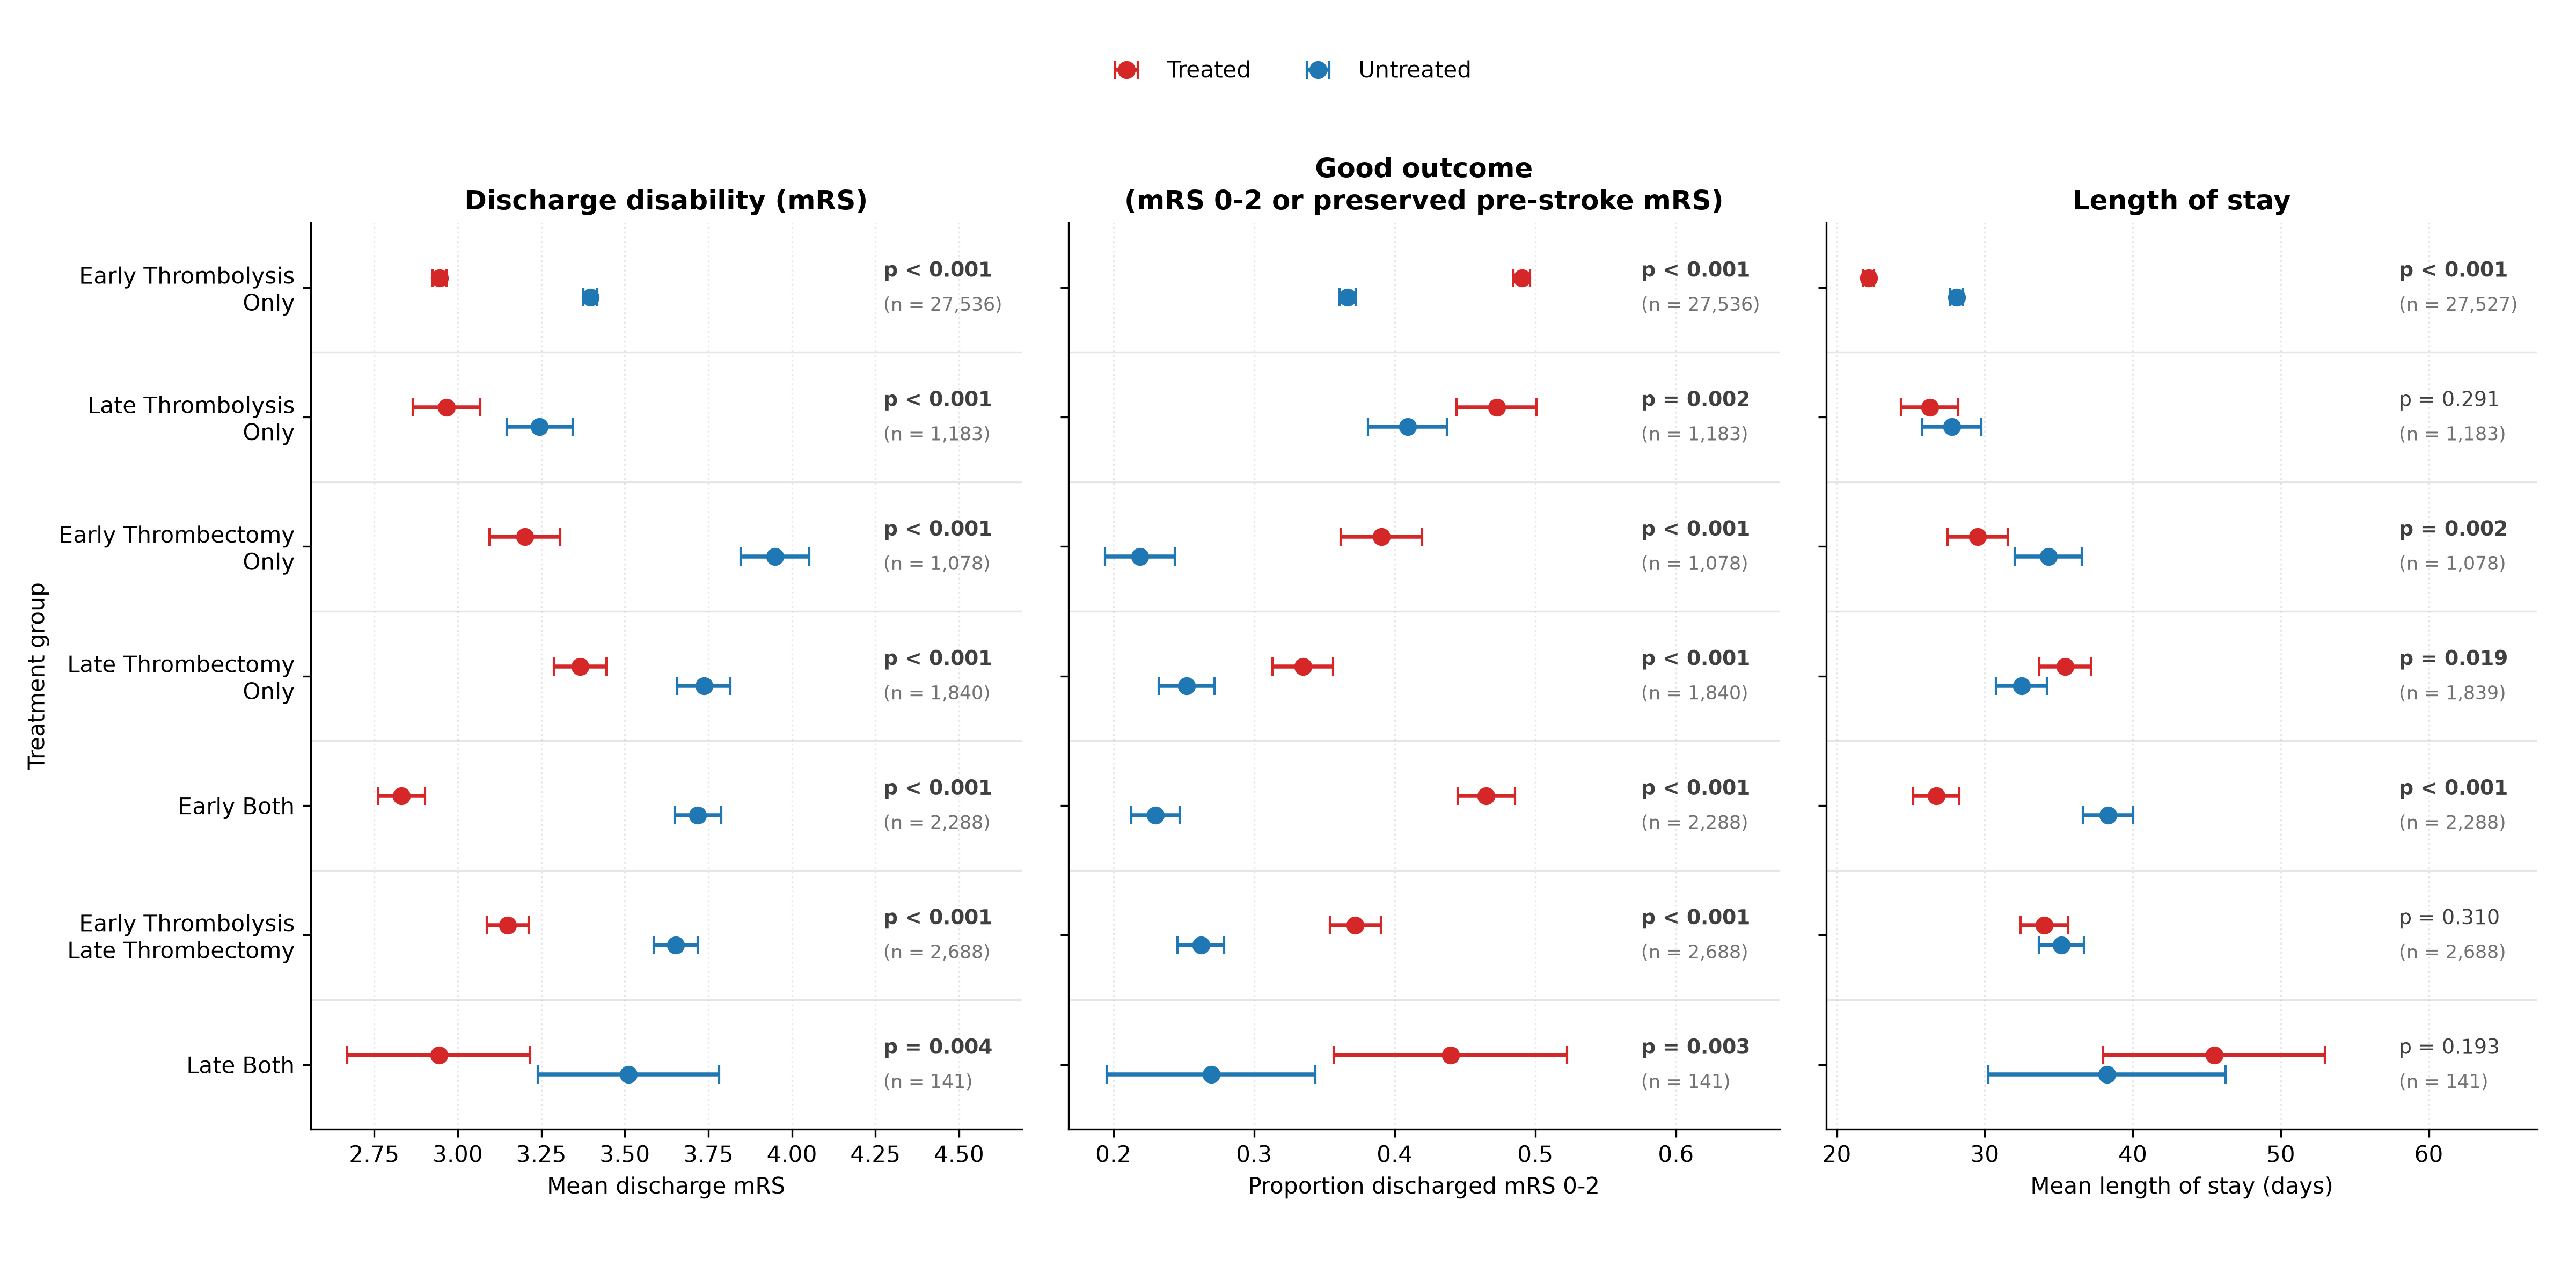
\includegraphics[width=1\linewidth]{images/treatment_effects/target_trial_emulation_mrs_2.png}
    \caption{Target trial emulation of reperfusion-treatment timing strategies and discharge functional outcomes, using matched control and treated patients. Estimated mean discharge modified Rankin Scale (mRS; left panel) and proportion achieving a good outcome at the mRS 0–2 threshold (right panel) are shown for patients receiving each treatment strategy (red) and their emulated untreated comparators (blue). Strategies are defined by early ($\leq$ 270 mins from onset) or late ($>$ 270 mins from onset) intravenous thrombolysis, mechanical thrombectomy, or their combination. Points denote estimated outcomes and horizontal bars 95\% confidence intervals; p-values indicate the treated–untreated comparison within each emulated treatment group, with sample sizes shown. Lower mRS and higher proportions with a good outcome indicate more favourable outcomes.}
    \label{fig:target_trial_mrs_2}
\end{figure}

\begin{figure}
    \centering
    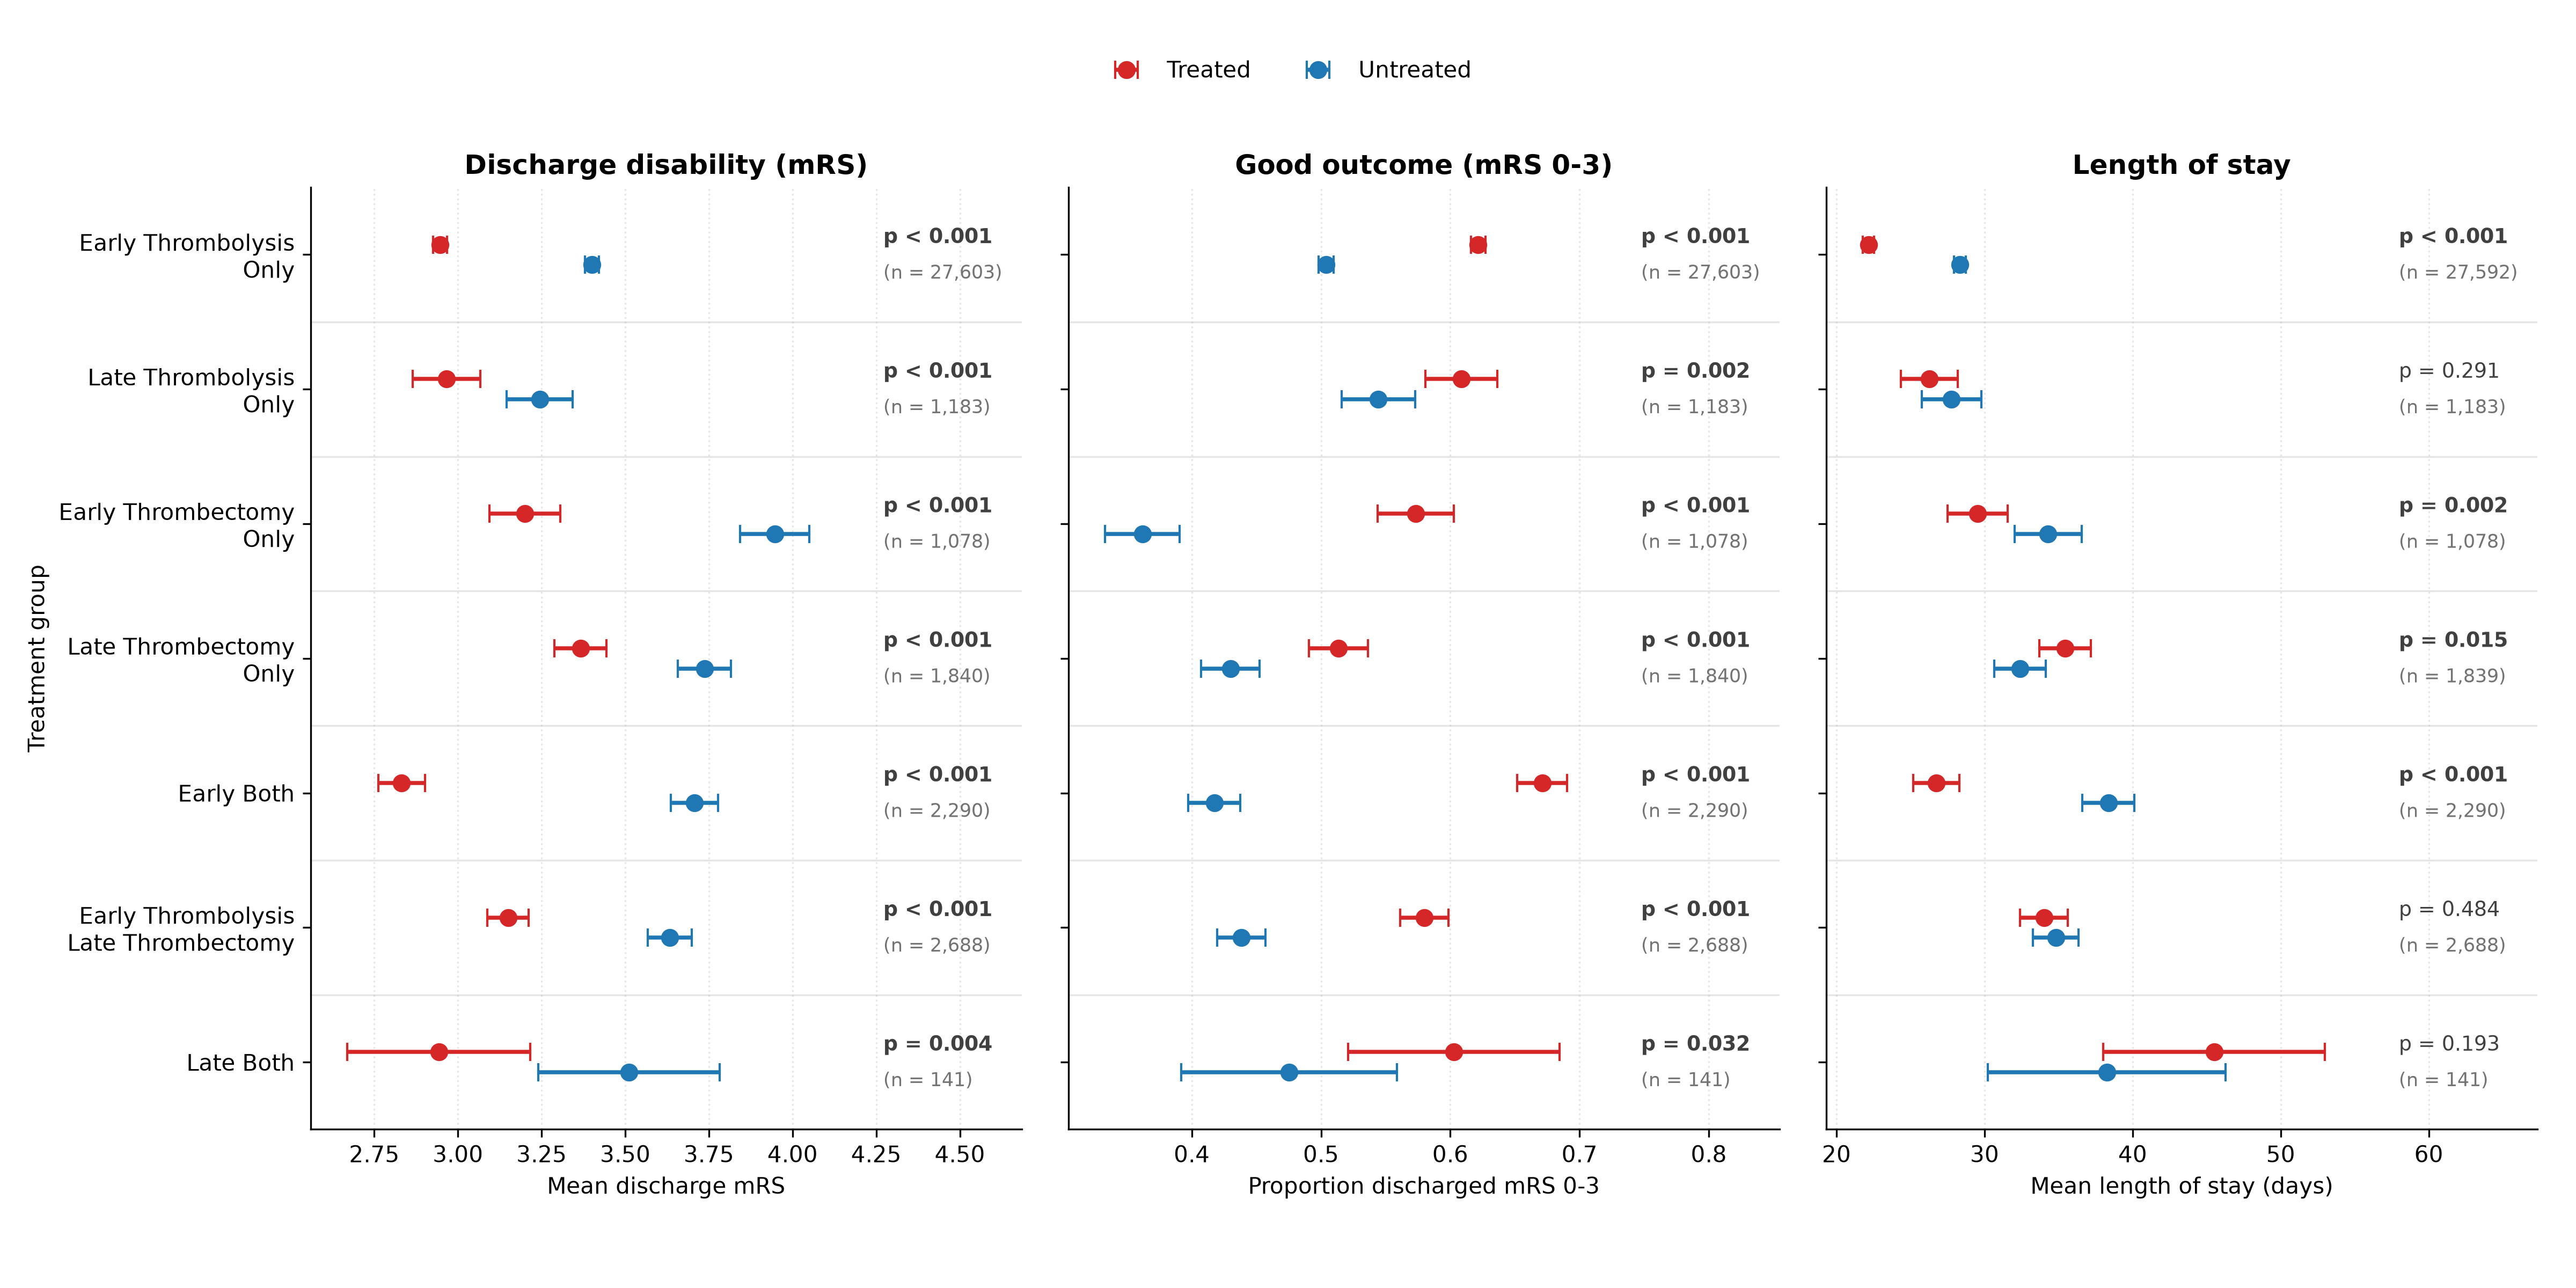
\includegraphics[width=1\linewidth]{images/treatment_effects/target_trial_emulation_mrs_3.png}
    \caption{Target trial emulation of reperfusion-treatment timing strategies and discharge functional outcomes, using matched control and treated patients. Estimated mean discharge modified Rankin Scale (mRS; left panel) and proportion achieving a good outcome at the mRS 0–3 threshold (right panel) are shown for patients receiving each treatment strategy (red) and their emulated untreated comparators (blue). Strategies are defined by early ($\leq$ 270 mins from onset) or late ($>$ 270 mins from onset) intravenous thrombolysis, mechanical thrombectomy, or their combination. Points denote estimated outcomes and horizontal bars 95\% confidence intervals; p-values indicate the treated–untreated comparison within each emulated treatment group, with sample sizes shown. Lower mRS and higher proportions with a good outcome indicate more favourable outcomes.}
    \label{fig:target_trial_mrs_3}
\end{figure}

\begin{figure}
    \centering
    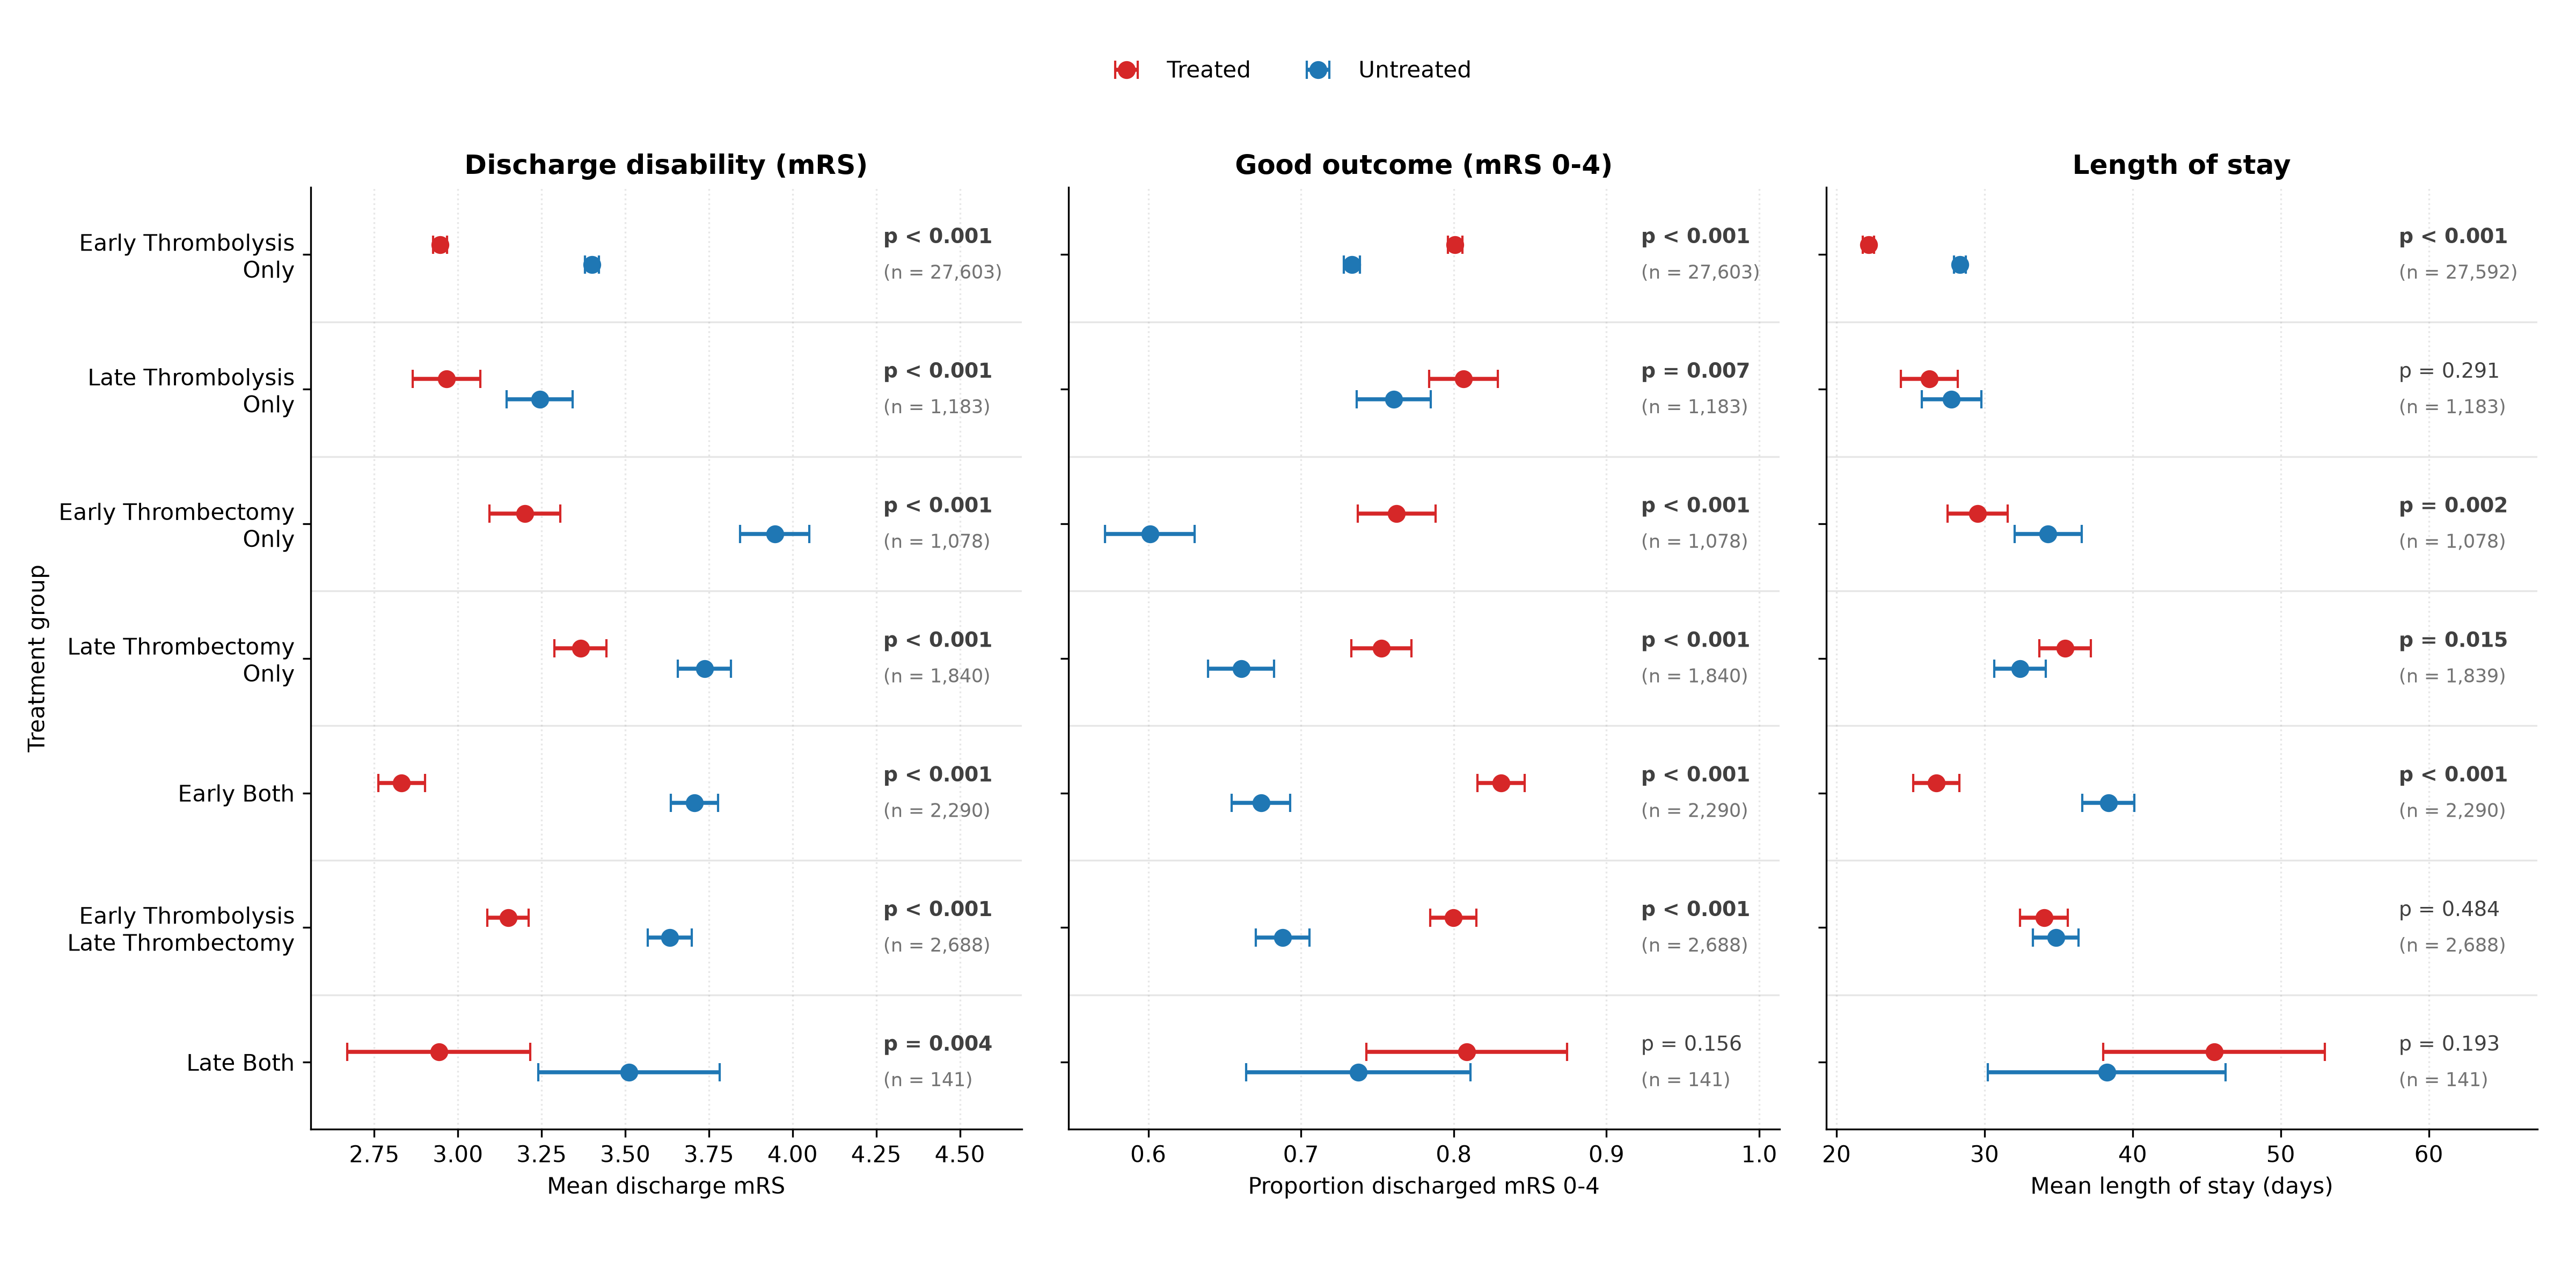
\includegraphics[width=1\linewidth]{images/treatment_effects/target_trial_emulation_mrs_4.png}
    \caption{Target trial emulation of reperfusion-treatment timing strategies and discharge functional outcomes, using matched control and treated patients. Estimated mean discharge modified Rankin Scale (mRS; left panel) and proportion achieving a good outcome at the mRS 0–4 threshold (right panel) are shown for patients receiving each treatment strategy (red) and their emulated untreated comparators (blue). Strategies are defined by early ($\leq$ 270 mins from onset) or late ($>$ 270 mins from onset) intravenous thrombolysis, mechanical thrombectomy, or their combination. Points denote estimated outcomes and horizontal bars 95\% confidence intervals; p-values indicate the treated–untreated comparison within each emulated treatment group, with sample sizes shown. Lower mRS and higher proportions with a good outcome indicate more favourable outcomes.}
    \label{fig:target_trial_mrs_4}
\end{figure}

\begin{figure}
    \centering
    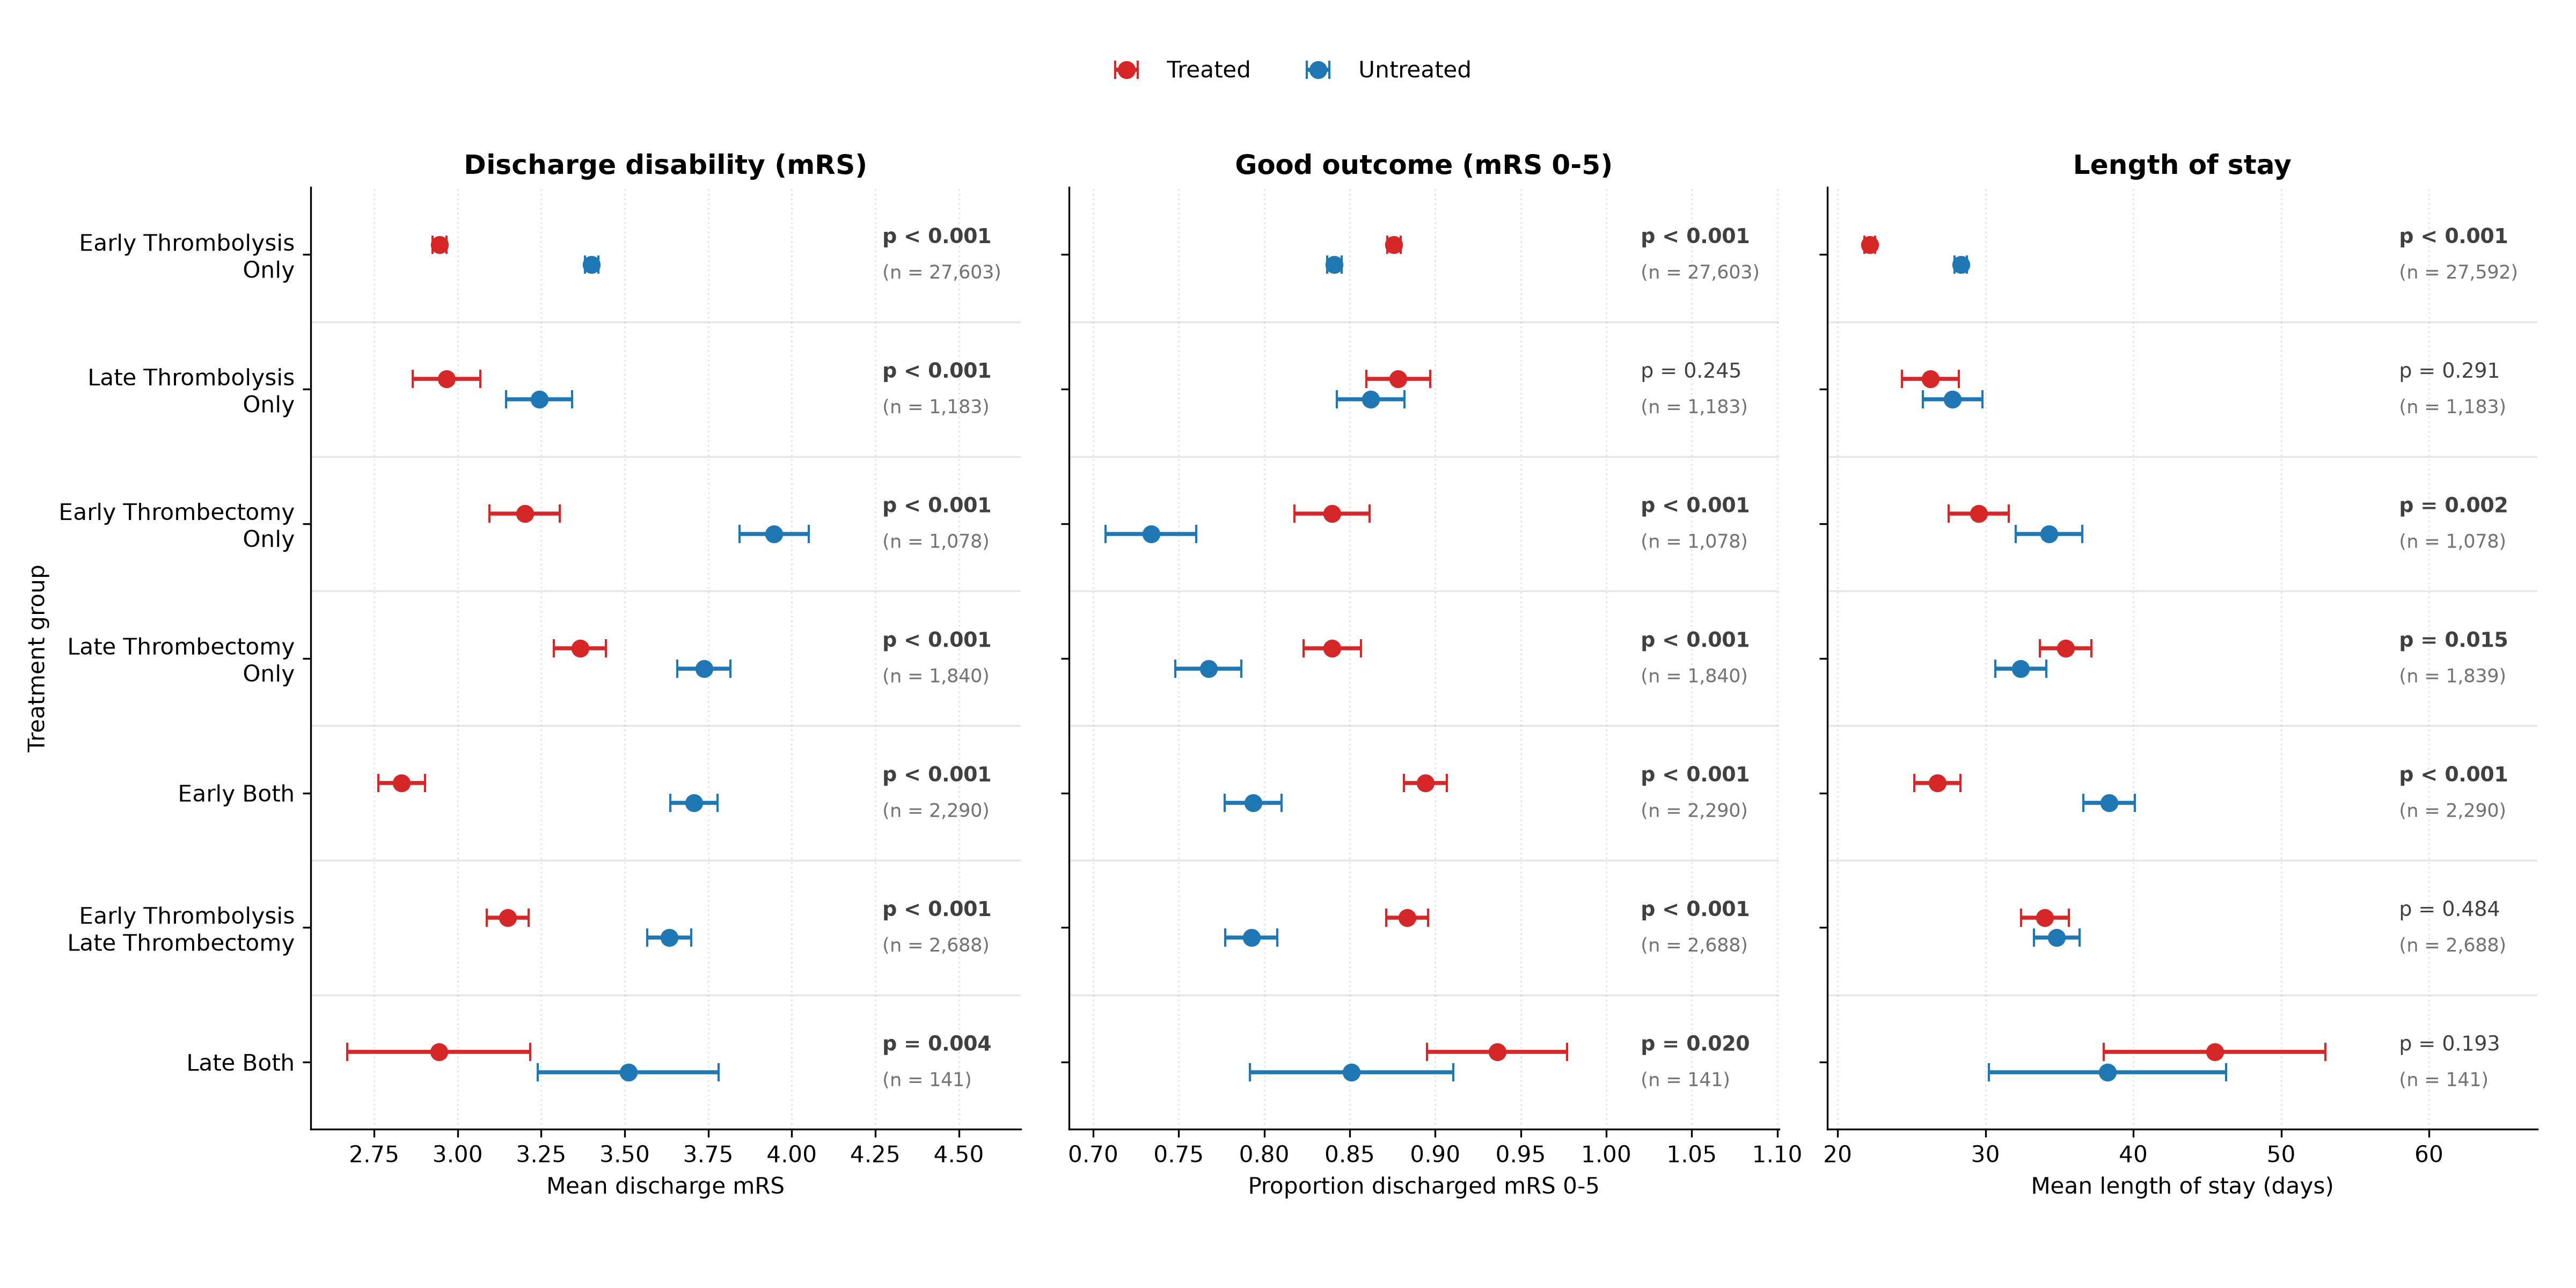
\includegraphics[width=1\linewidth]{images/treatment_effects/target_trial_emulation_mrs_5.png}
    \caption{Target trial emulation of reperfusion-treatment timing strategies and discharge functional outcomes, using matched control and treated patients. Estimated mean discharge modified Rankin Scale (mRS; left panel) and proportion achieving a good outcome at the mRS 0–5 threshold (survival, right panel) are shown for patients receiving each treatment strategy (red) and their emulated untreated comparators (blue). Strategies are defined by early ($\leq$ 270 mins from onset) or late ($>$ 270 mins from onset) intravenous thrombolysis, mechanical thrombectomy, or their combination. Points denote estimated outcomes and horizontal bars 95\% confidence intervals; p-values indicate the treated–untreated comparison within each emulated treatment group, with sample sizes shown. Lower mRS and higher proportions with a good outcome indicate more favourable outcomes.}
    \label{fig:target_trial_mrs_5}
\end{figure}

% ------------------------------------------------------------------------------------

\newpage

\subsection{S-learner}

Figure \ref{fig:s_learner_benefit} shows treatment effects estimated by the XGBoost S-learner for each mRS threshold. For each treated patient, the model predicted the outcome both with the treatment actually received and with no reperfusion treatment; the difference between these two predictions is that patient's estimated treatment effect. Treatment effects are shown as log odds ratios (treated vs.\ untreated) for achieving the outcome, averaged over patients in each treatment group. A value of zero indicates no effect, positive values indicate benefit, and a log odds ratio of about 0.69 corresponds to a doubling of the odds. Treatment type and timing (early vs.\ late, using a 270-minute onset-to-treatment threshold) were coded as a single categorical feature for this model.

%%%%%%%%%%%%%%%%%%%%%%%%%%%%%%%%%%%%%%%%%%

\begin{figure}
    \centering
    
    % Top left
    \begin{subfigure}{0.48\textwidth}
        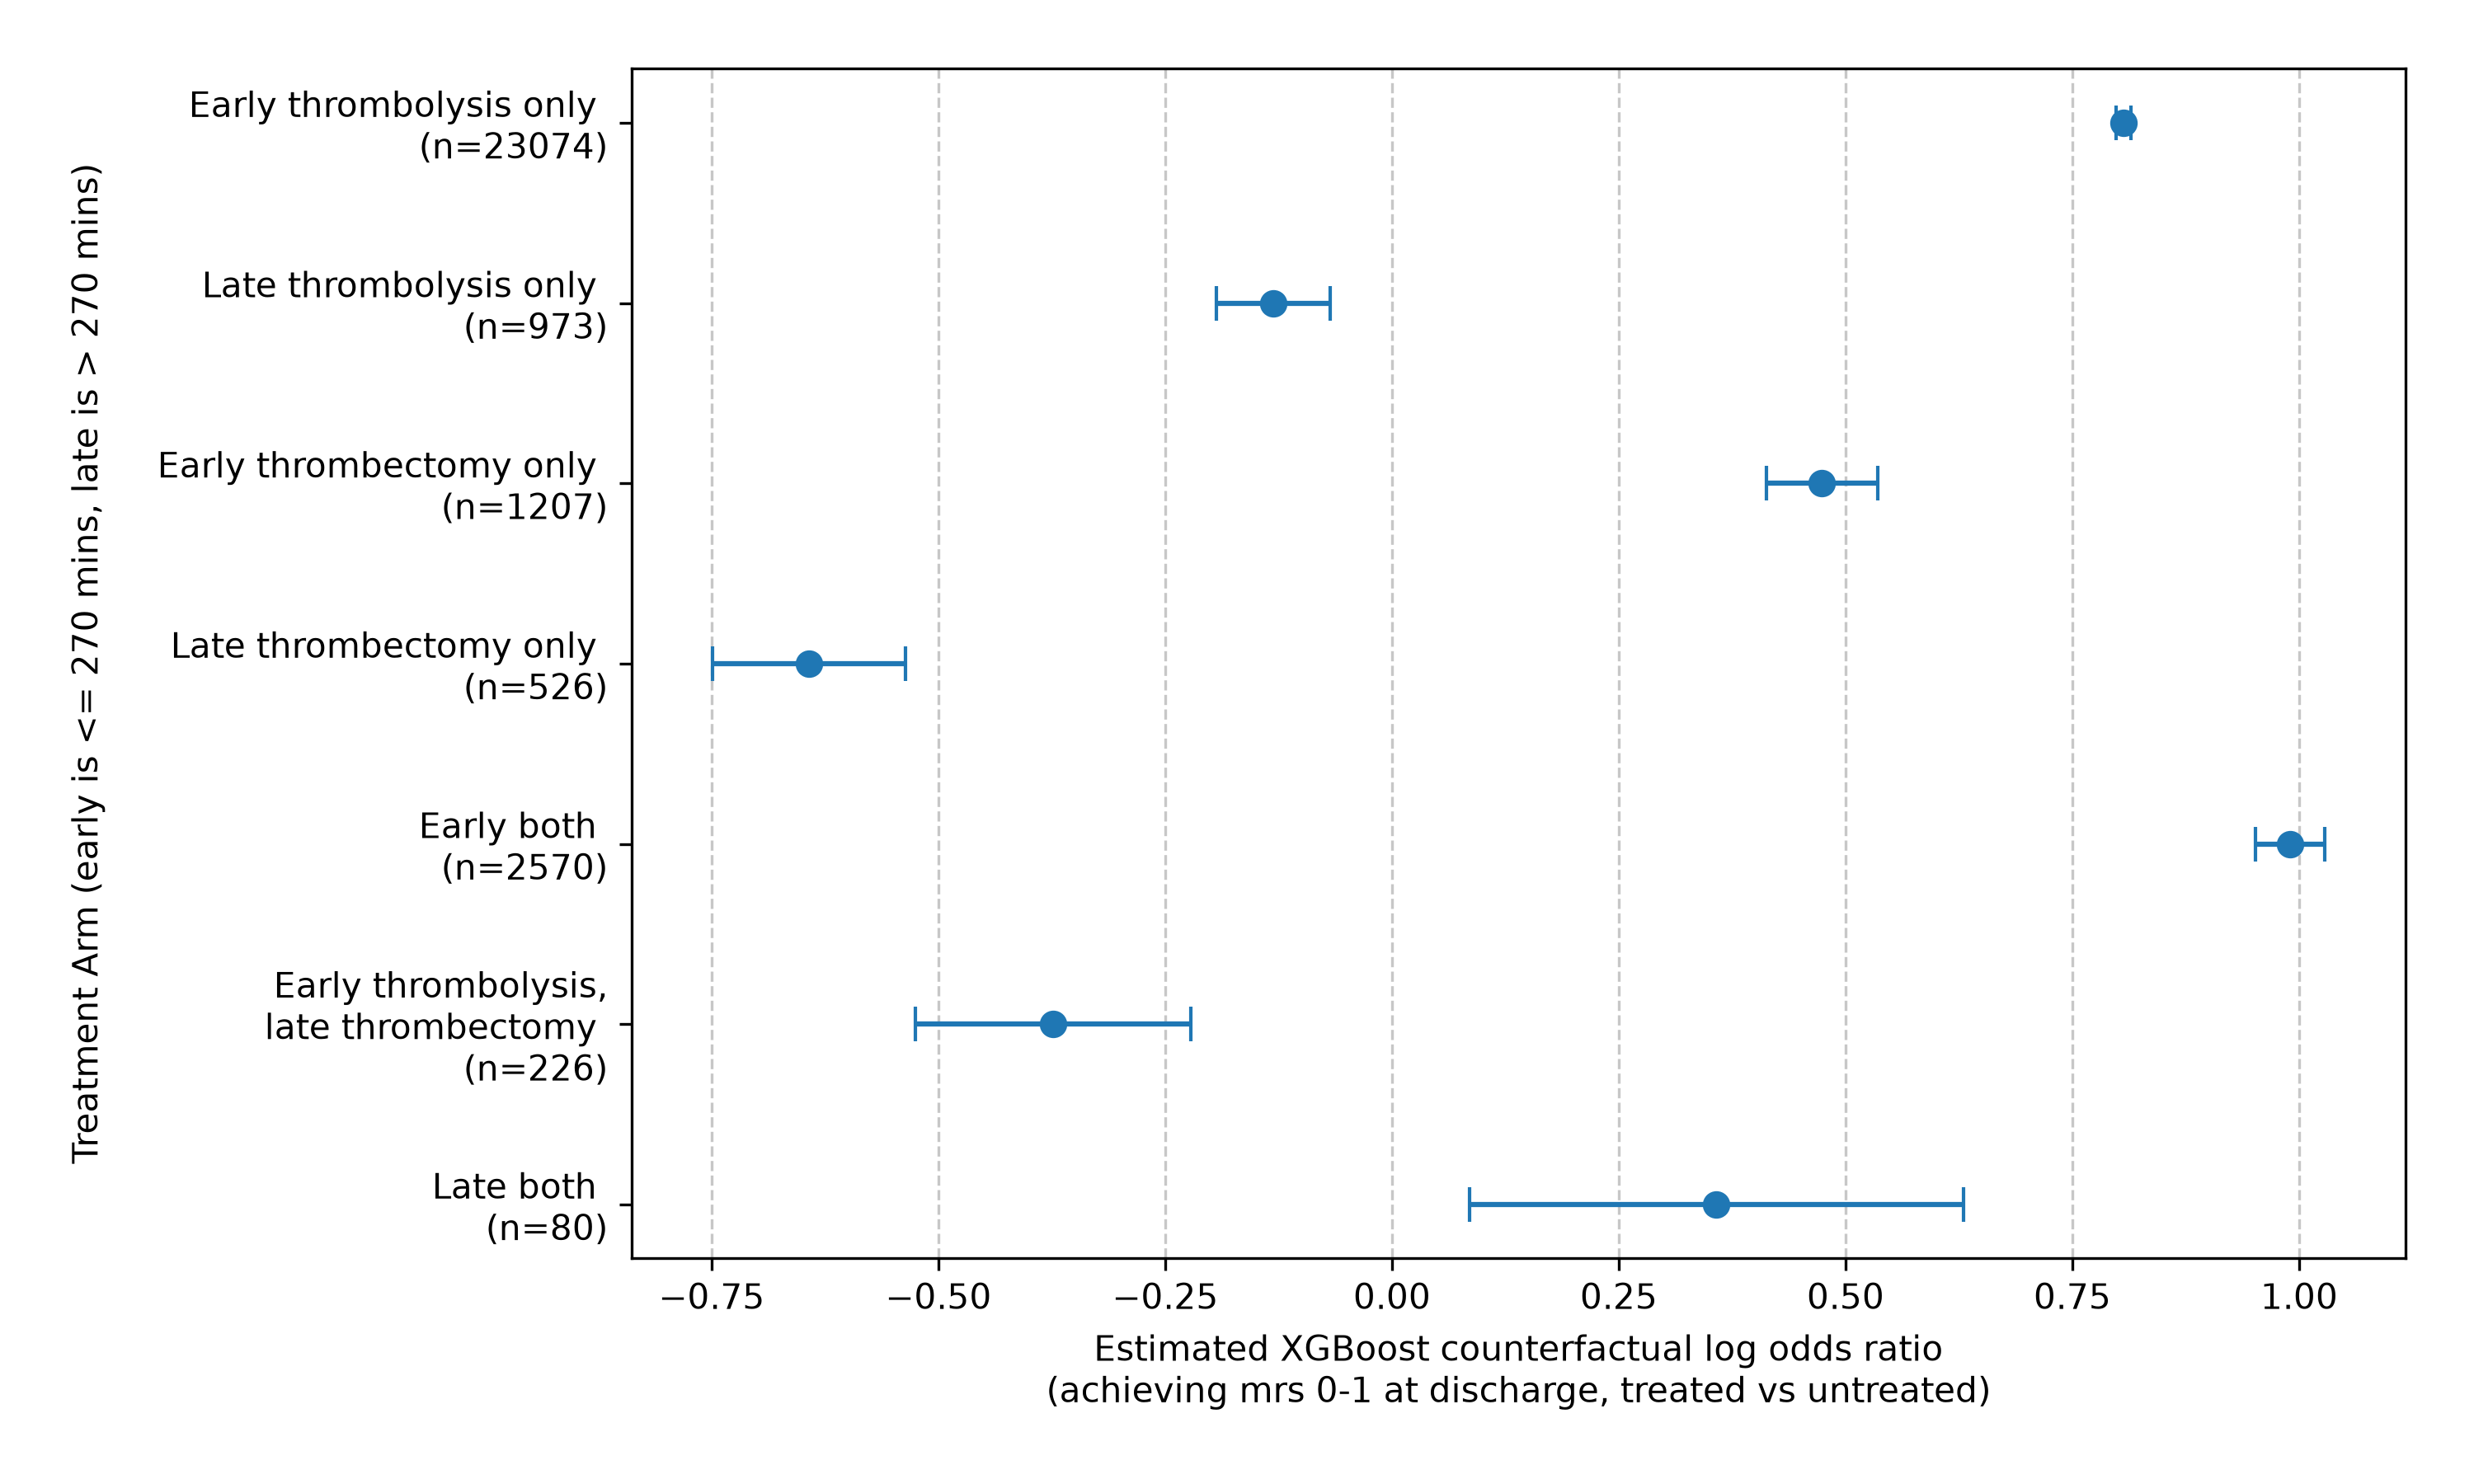
\includegraphics[width=\linewidth]{images/treatment_effects/xgboost_counterfactual_cate_log_odds_estimates_1.png}
        %\caption{}
    \end{subfigure}
    \hfill % Adds flexible horizontal spacing
    % top right image 
    \begin{subfigure}{0.48\textwidth}
        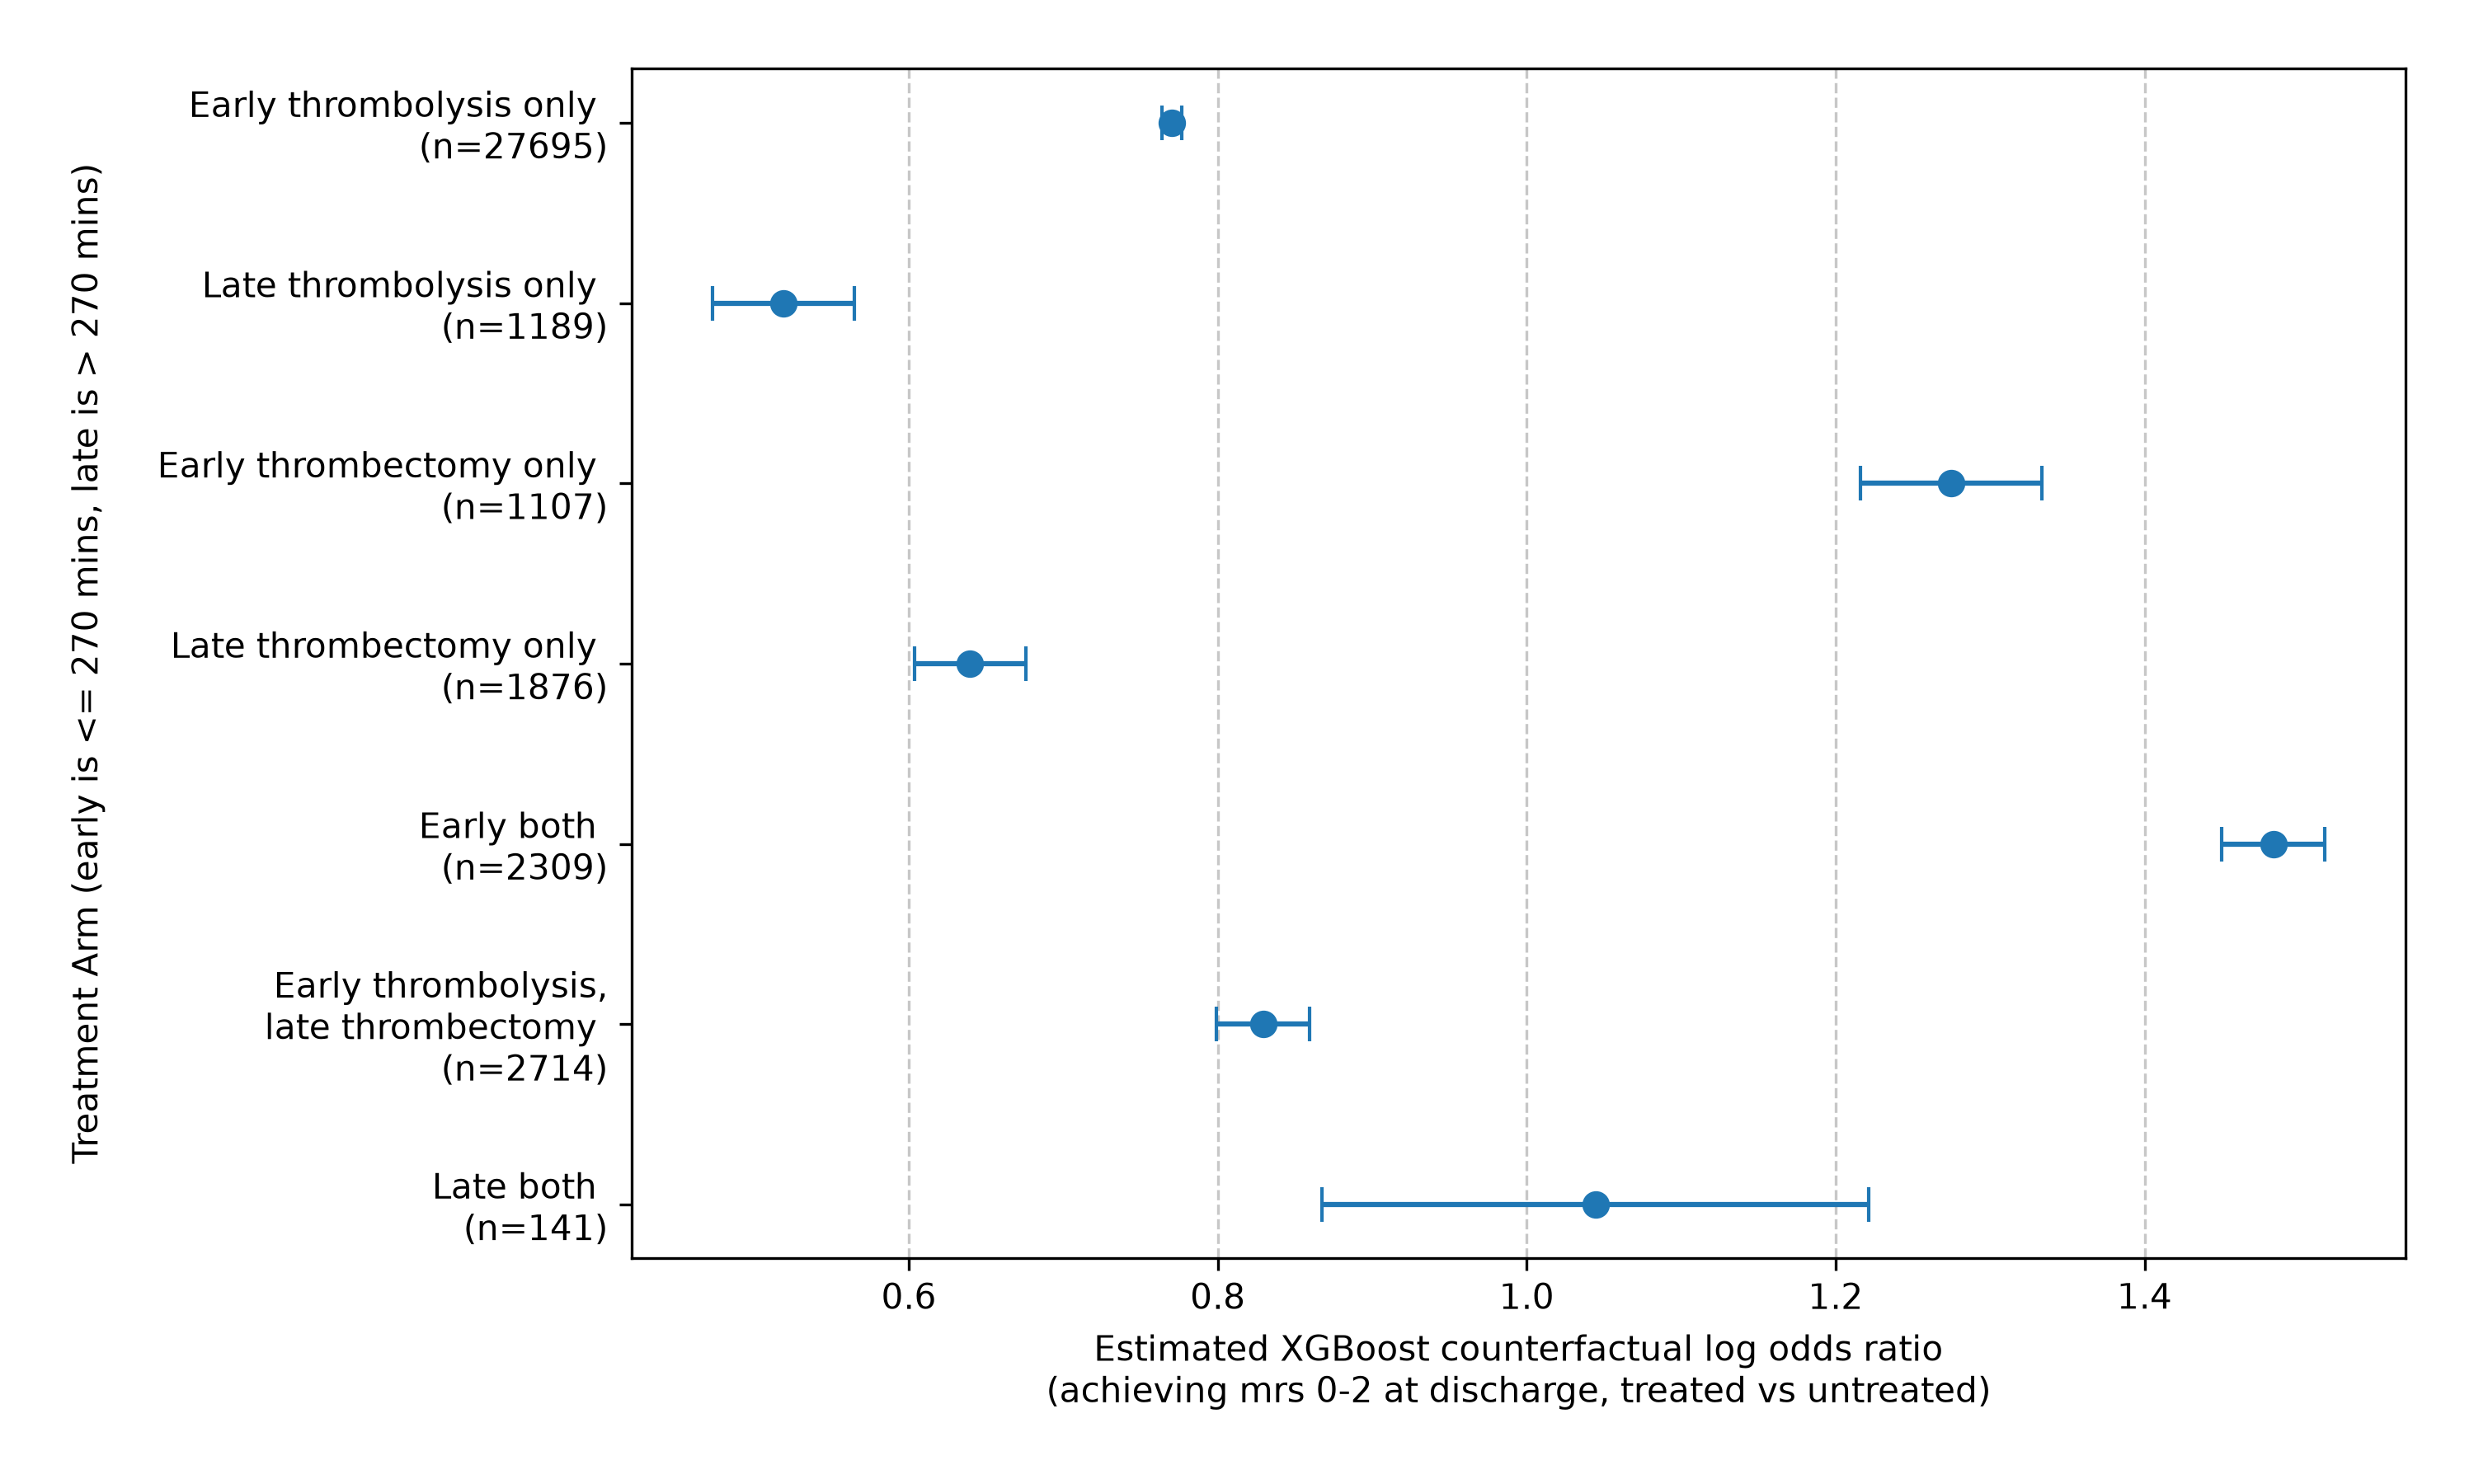
\includegraphics[width=\linewidth]{images/treatment_effects/xgboost_counterfactual_cate_log_odds_estimates_2.png}
        %\caption{}
    \end{subfigure}

    \vspace{0.5cm} % Optional vertical space between rows

    % Center left image
    \begin{subfigure}{0.48\textwidth}
        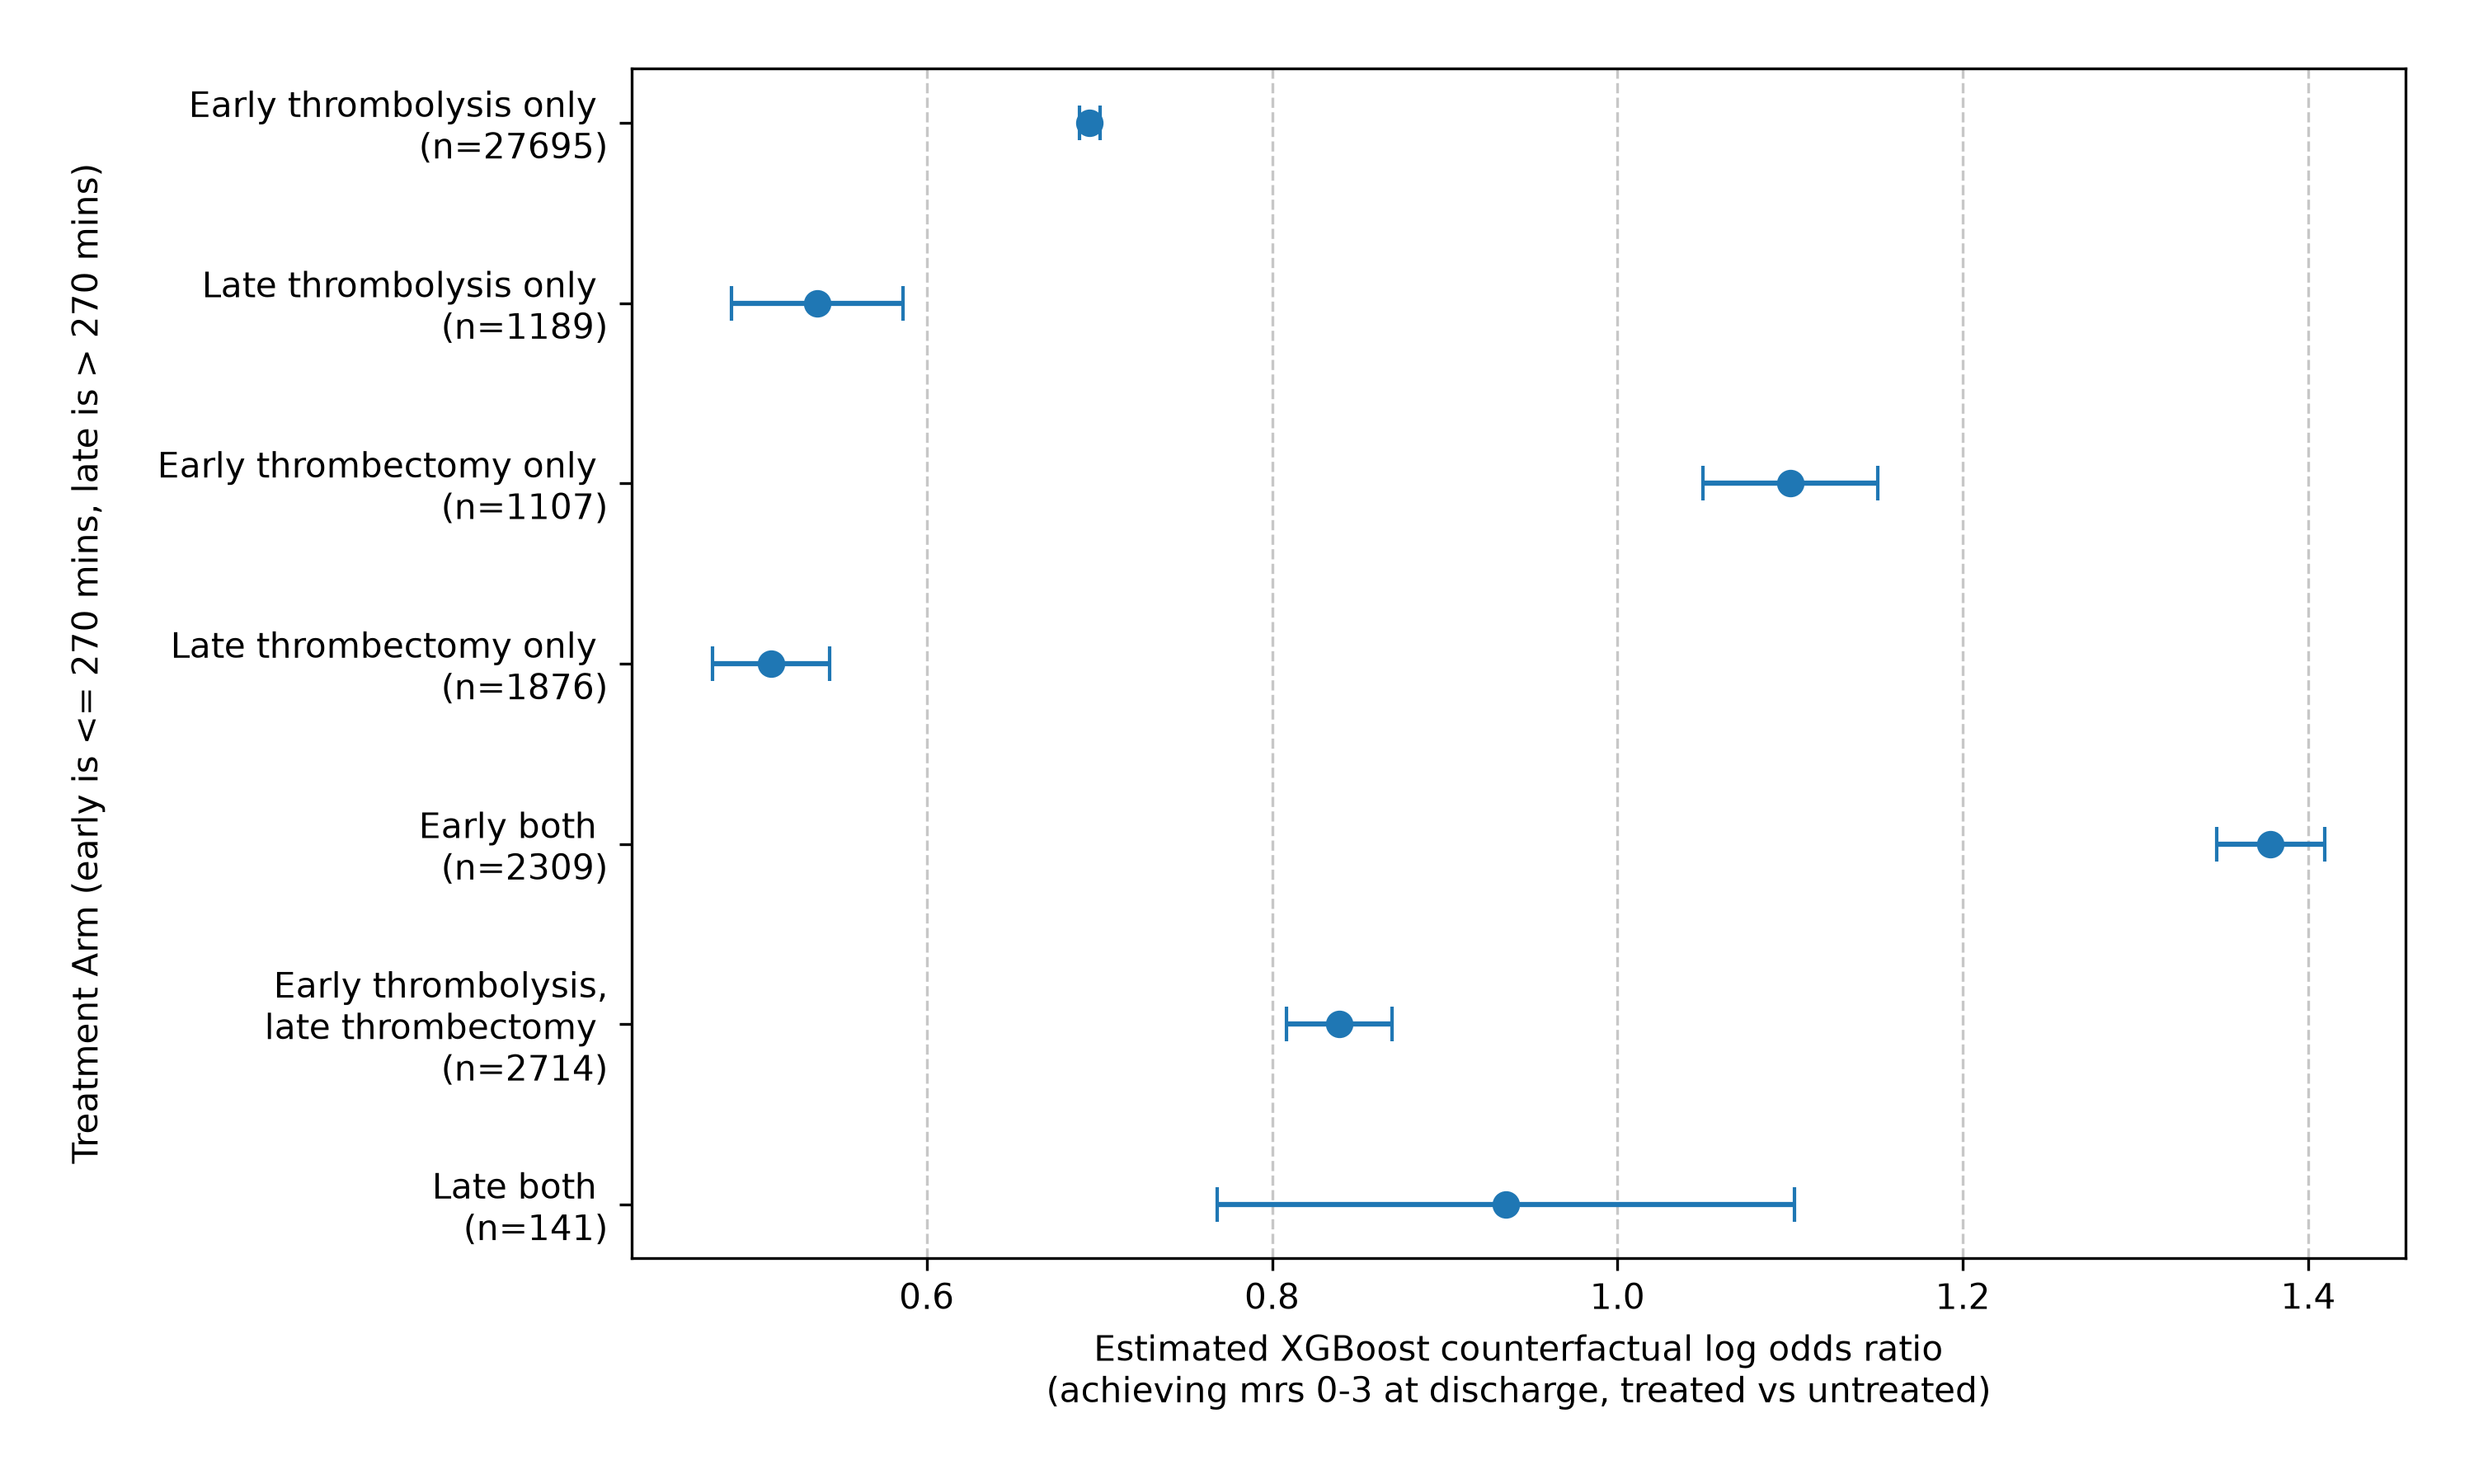
\includegraphics[width=\linewidth]{images/treatment_effects/xgboost_counterfactual_cate_log_odds_estimates_3}
        %\caption{}
    \end{subfigure}
    \hfill % Adds flexible horizontal spacing
    % Centre right image 
    \begin{subfigure}{0.48\textwidth}
        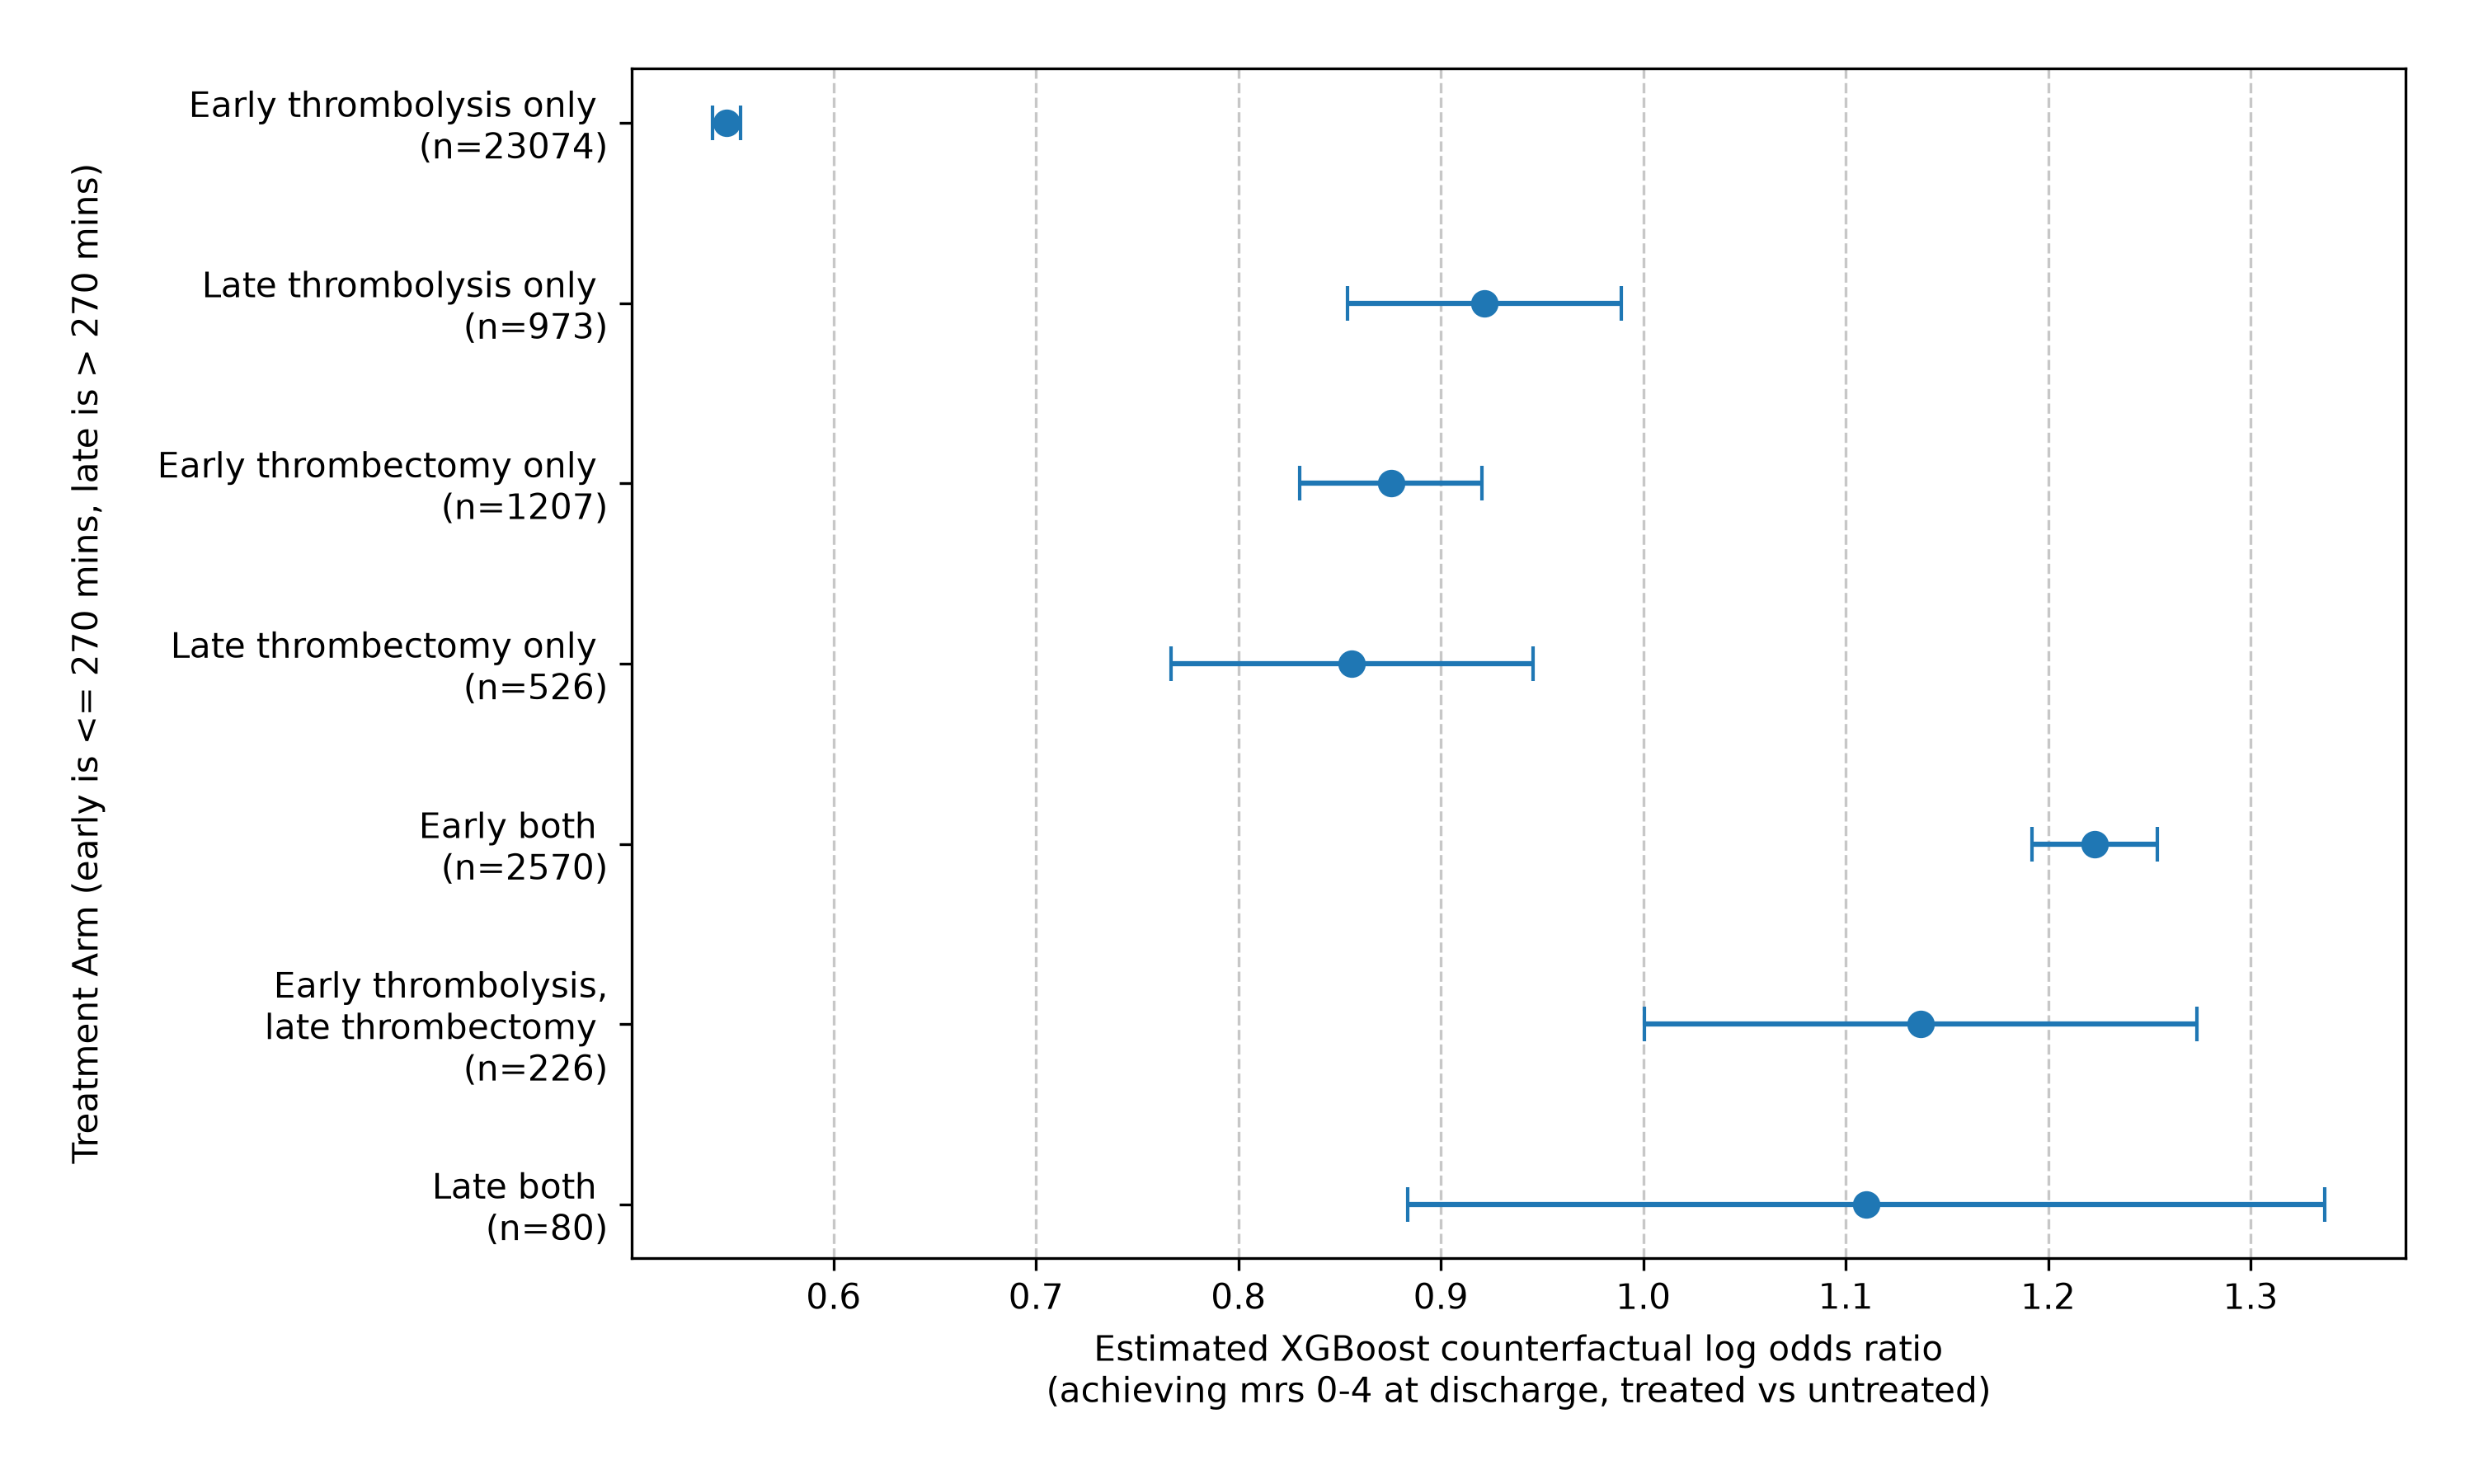
\includegraphics[width=\linewidth]{images/treatment_effects/xgboost_counterfactual_cate_log_odds_estimates_4}
        %\caption{}
    \end{subfigure}

    \vspace{0.5cm} % Optional vertical space between rows

    % Bottom image
    \begin{subfigure}{0.48\textwidth}
        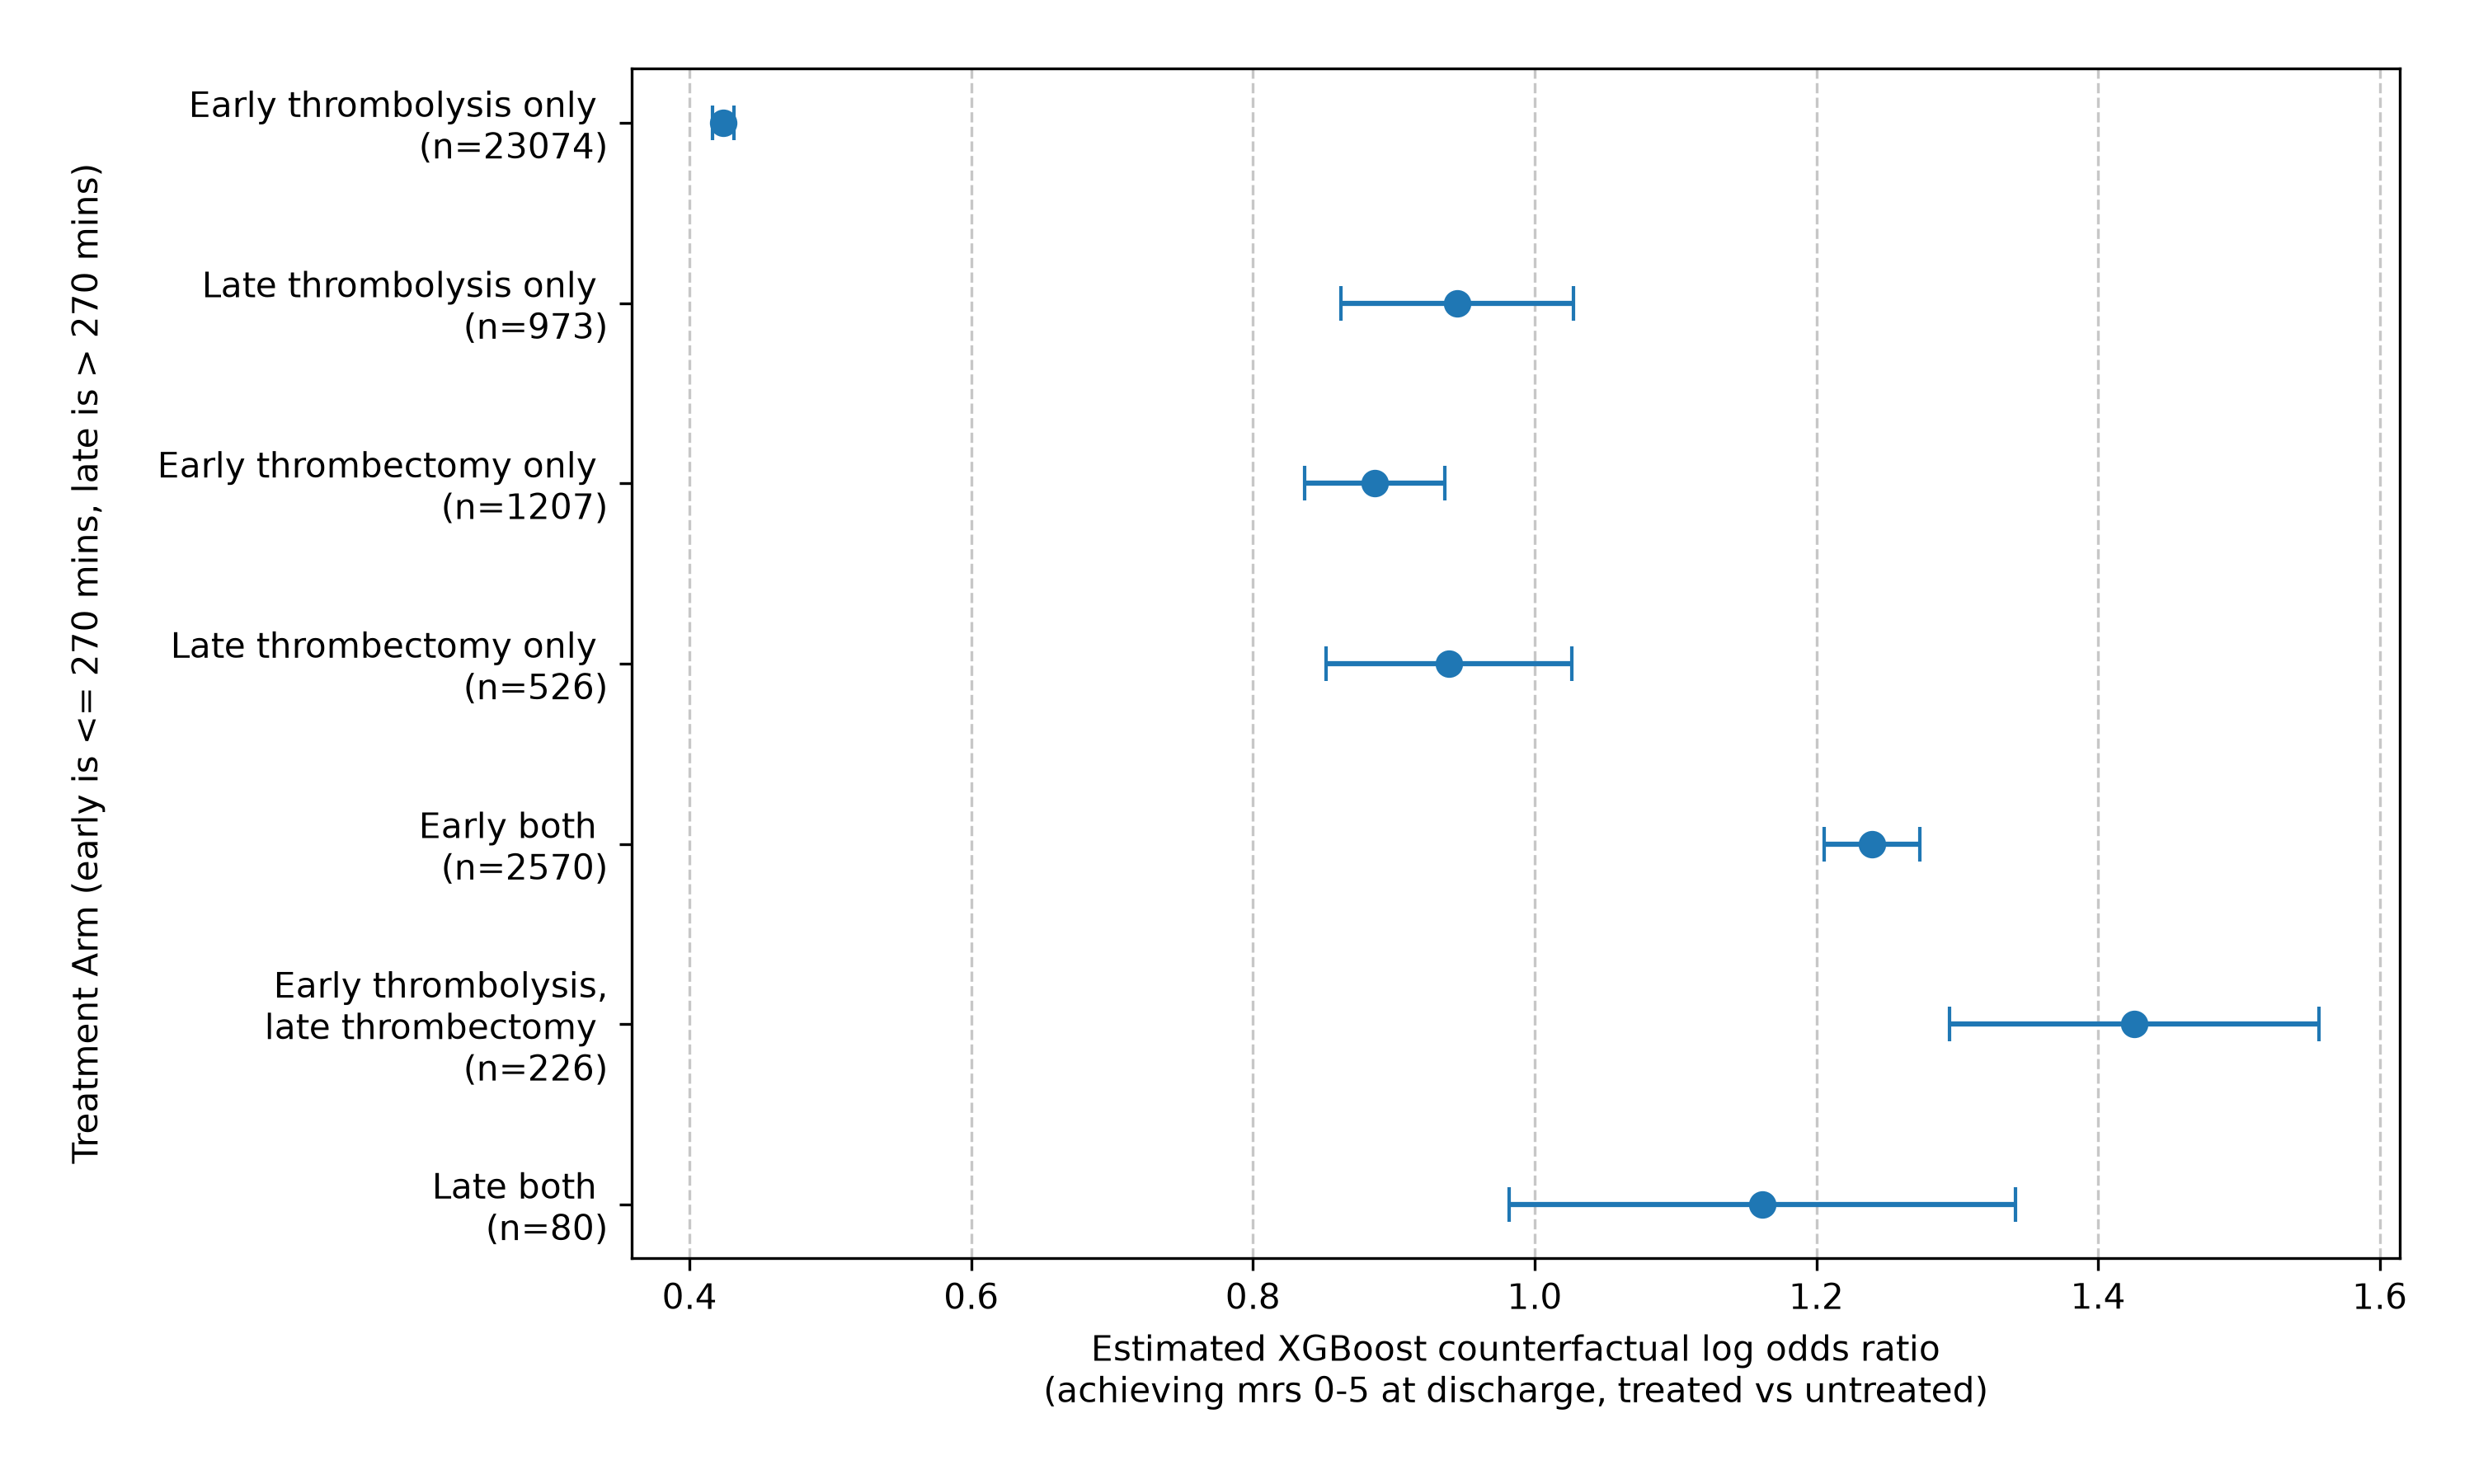
\includegraphics[width=\linewidth]{images/treatment_effects/xgboost_counterfactual_cate_log_odds_estimates_5}
        %\caption{}
    \end{subfigure}
    
    \caption{Estimated counterfactual treatment benefit across reperfusion-treatment timing strategies, derived from the XGBoost S-learner model. Each panel shows results for discharge at or below each modified Rankin Scale (mRS) level. Points represent the mean estimated individual treatment effect for each treatment-timing group, expressed as the counterfactual log odds ratio for the specified outcome relative to no reperfusion treatment; horizontal error bars show 95\% confidence intervals. Treatment groups are defined by receipt of intravenous thrombolysis and/or mechanical thrombectomy, with early treatment defined as onset-to-treatment time $<$270 minutes and late treatment as $\geq$270 minutes. Sample sizes are shown alongside group labels. Values above zero indicate a model-predicted increase in the odds of a good outcome at the corresponding threshold under the observed treatment strategy compared with no treatment.}
    \label{fig:s_learner_benefit}
\end{figure}



%%%%%%%%%%%%%%%%%%%%%%%%%%%%%%%%%%%%%%%%%%

Figure \ref{fig:s_learner_heatmap_log odds} shows a heatmap of the estimated benefit of thrombolysis and thrombectomy by use and speed in achieving each mRS threshold. This model used actual onset-to-treatment times for each of thrombolysis and thrombectomy, rather than early/late groups. The resulting benefit, estimated for each patient using counterfactual modelling, was then grouped by the time (in hours) of each treatment after stroke onset. Each cell gives the mean predicted benefit for patients whose thrombolysis and thrombectomy were given in that pair of hourly intervals, so reading along a row or down a column shows how benefit changes as one treatment is delayed while the timing of the other is held fixed. The final row and column show patients who received only one of the two treatments.

\begin{figure}[htbp]
    \centering
    
    % Top left
    \begin{subfigure}{0.48\textwidth}
        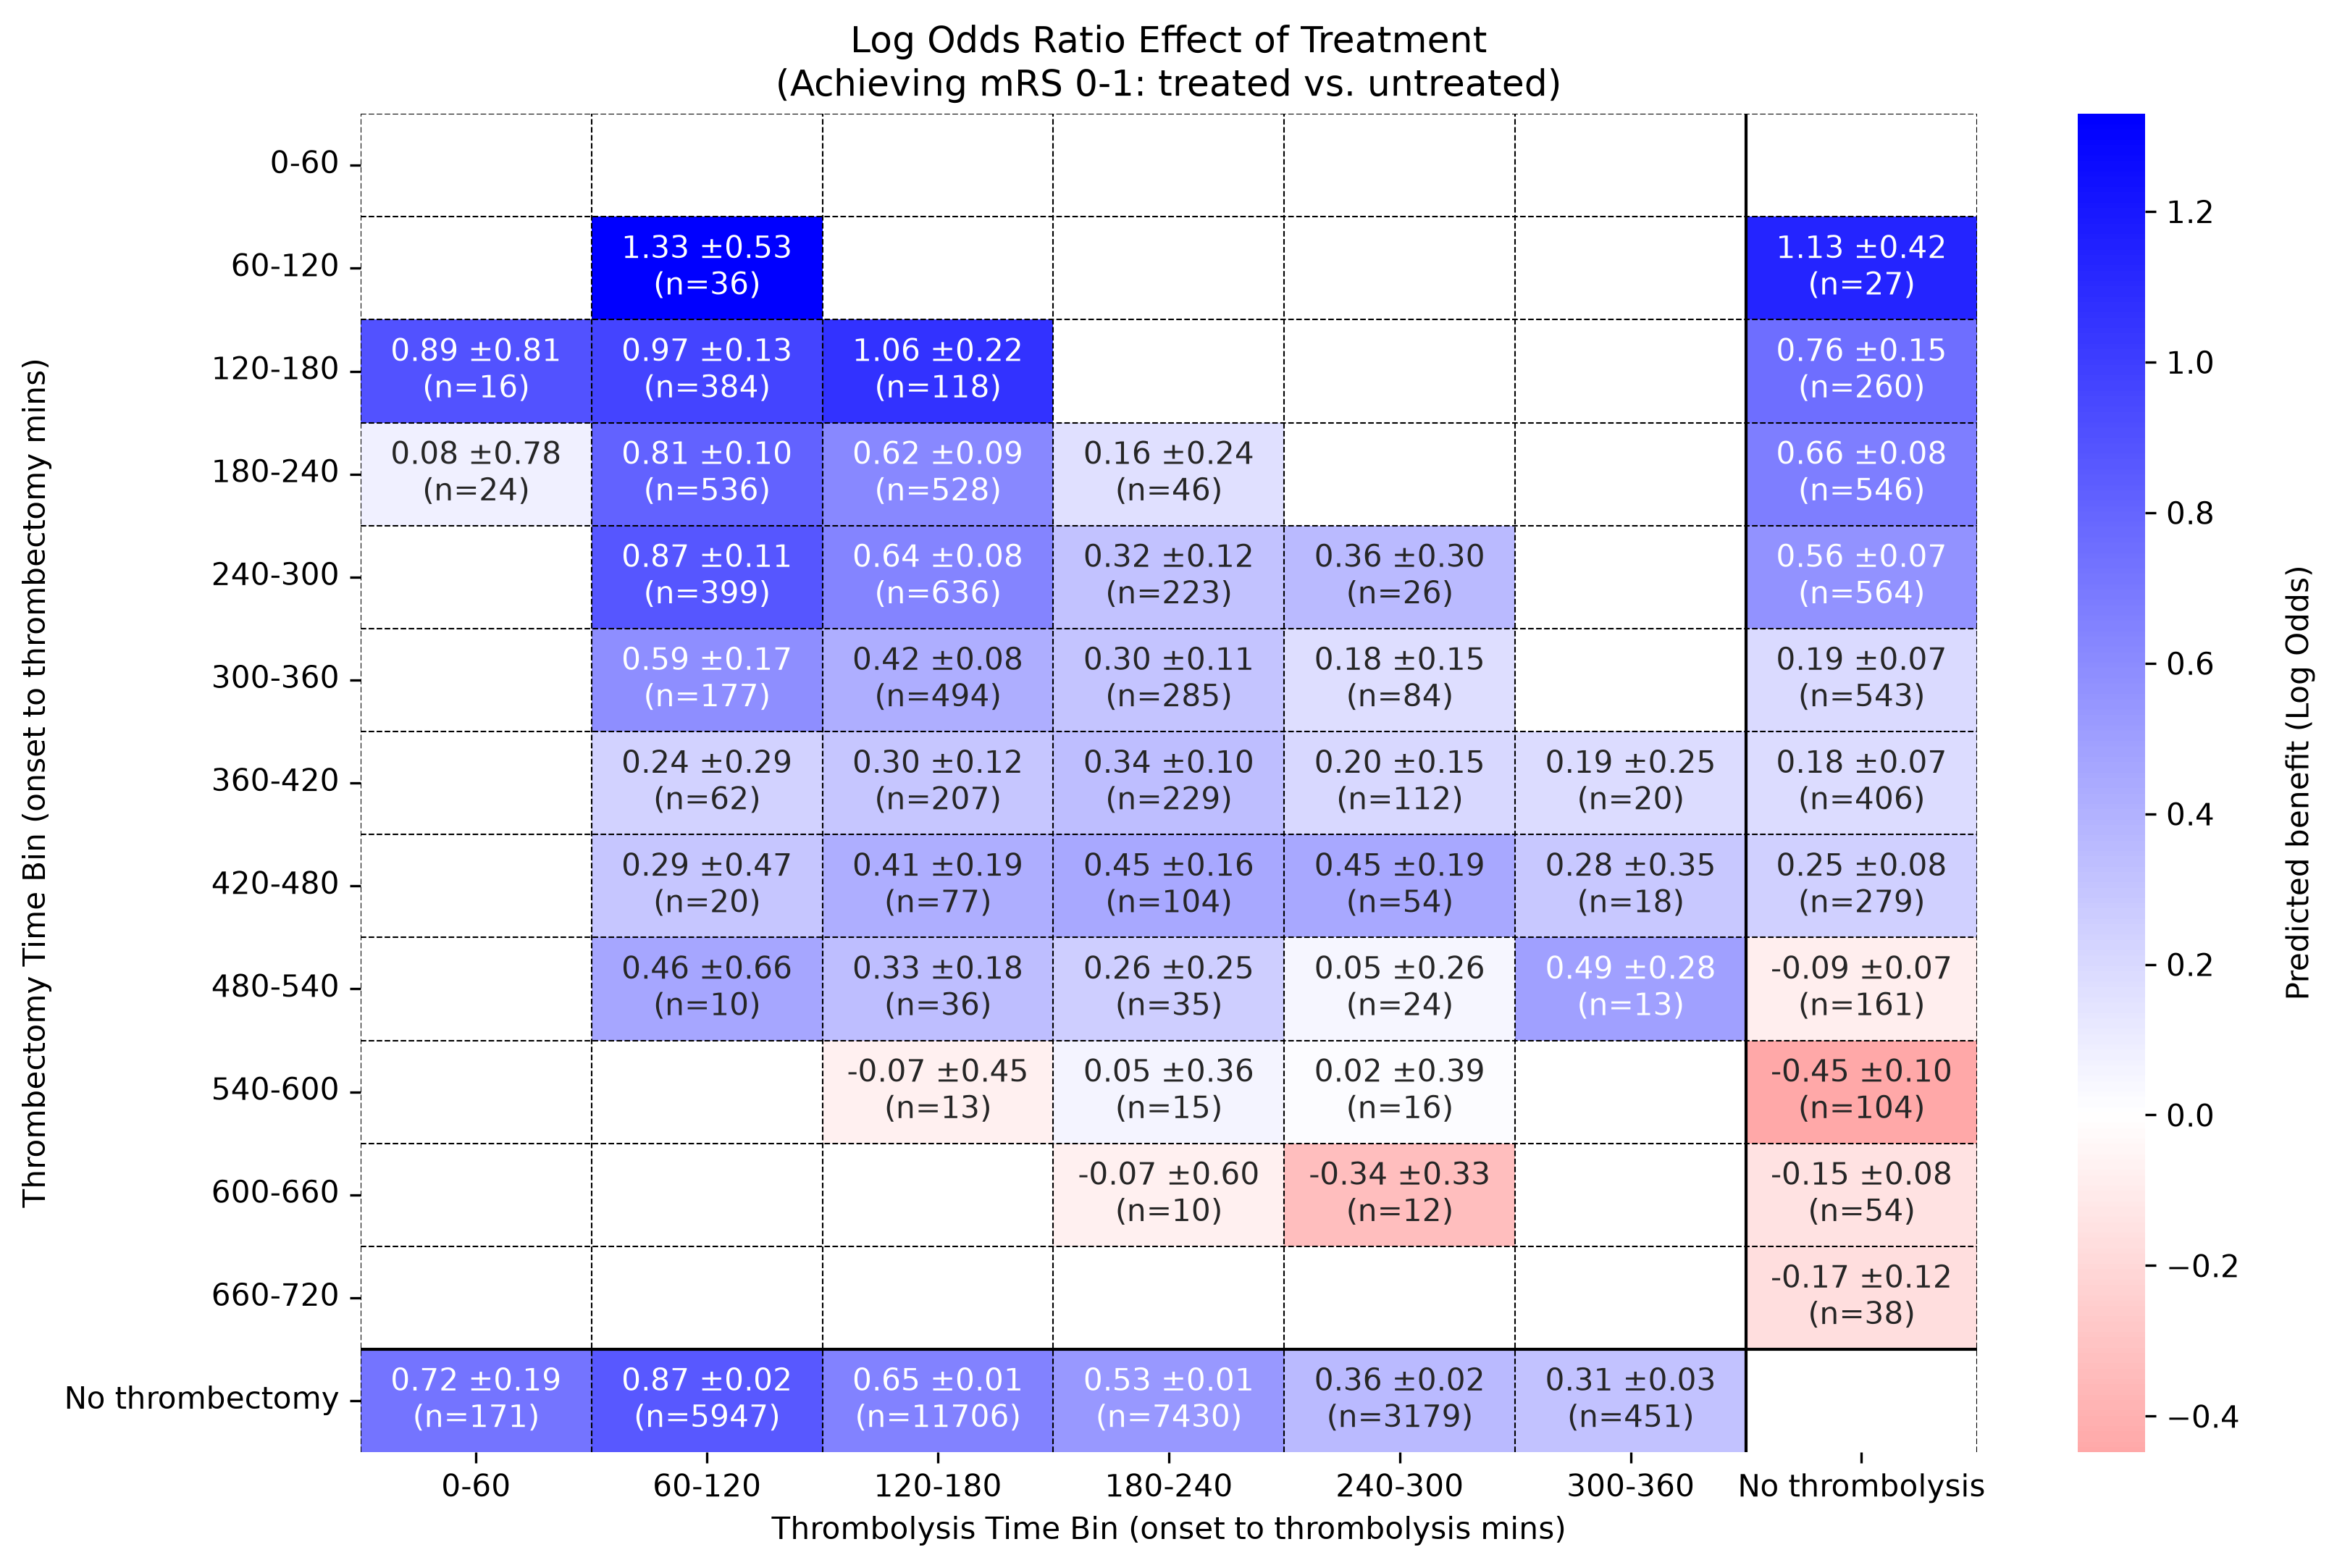
\includegraphics[width=\linewidth]{images/treatment_effects/thrombolysis_thrombectomy_heatmap_mrs_1.png}
        %\caption{}
    \end{subfigure}
    \hfill % Adds flexible horizontal spacing
    % top right image 
    \begin{subfigure}{0.48\textwidth}
        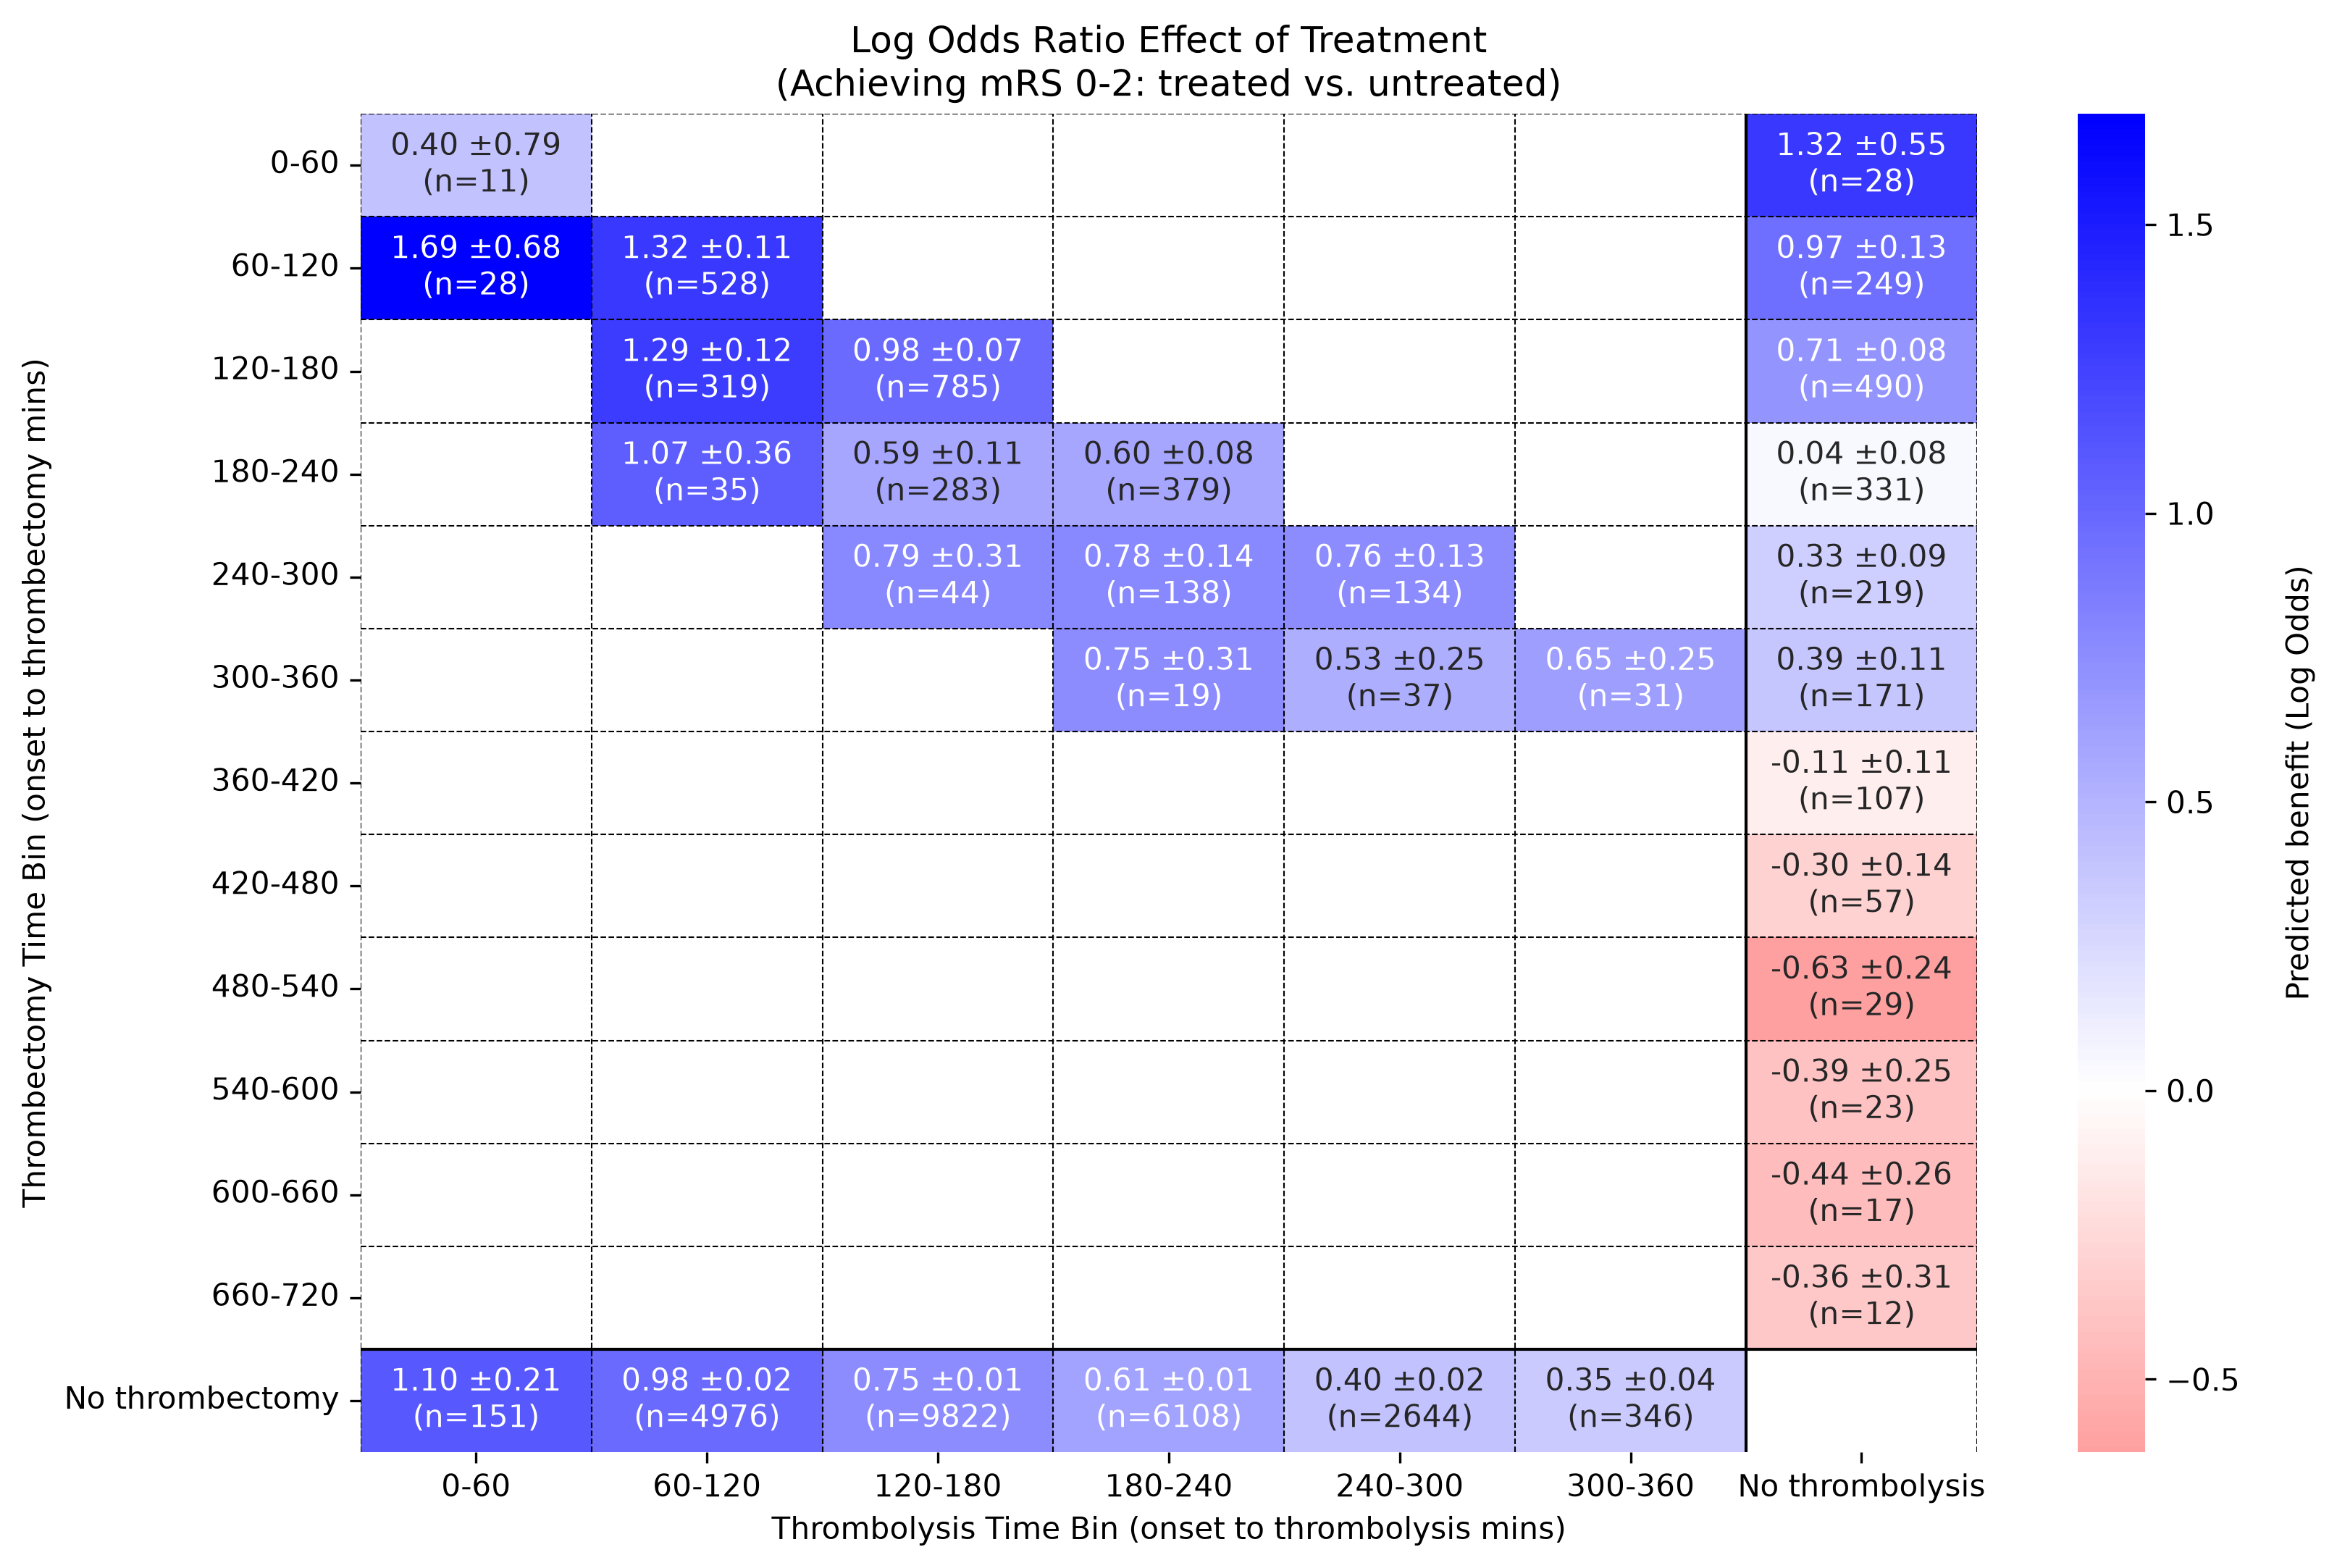
\includegraphics[width=\linewidth]{images/treatment_effects/thrombolysis_thrombectomy_heatmap_mrs_2.png}
        %\caption{}
    \end{subfigure}

    \vspace{0.5cm} % Optional vertical space between rows

    % Center left image
    \begin{subfigure}{0.48\textwidth}
        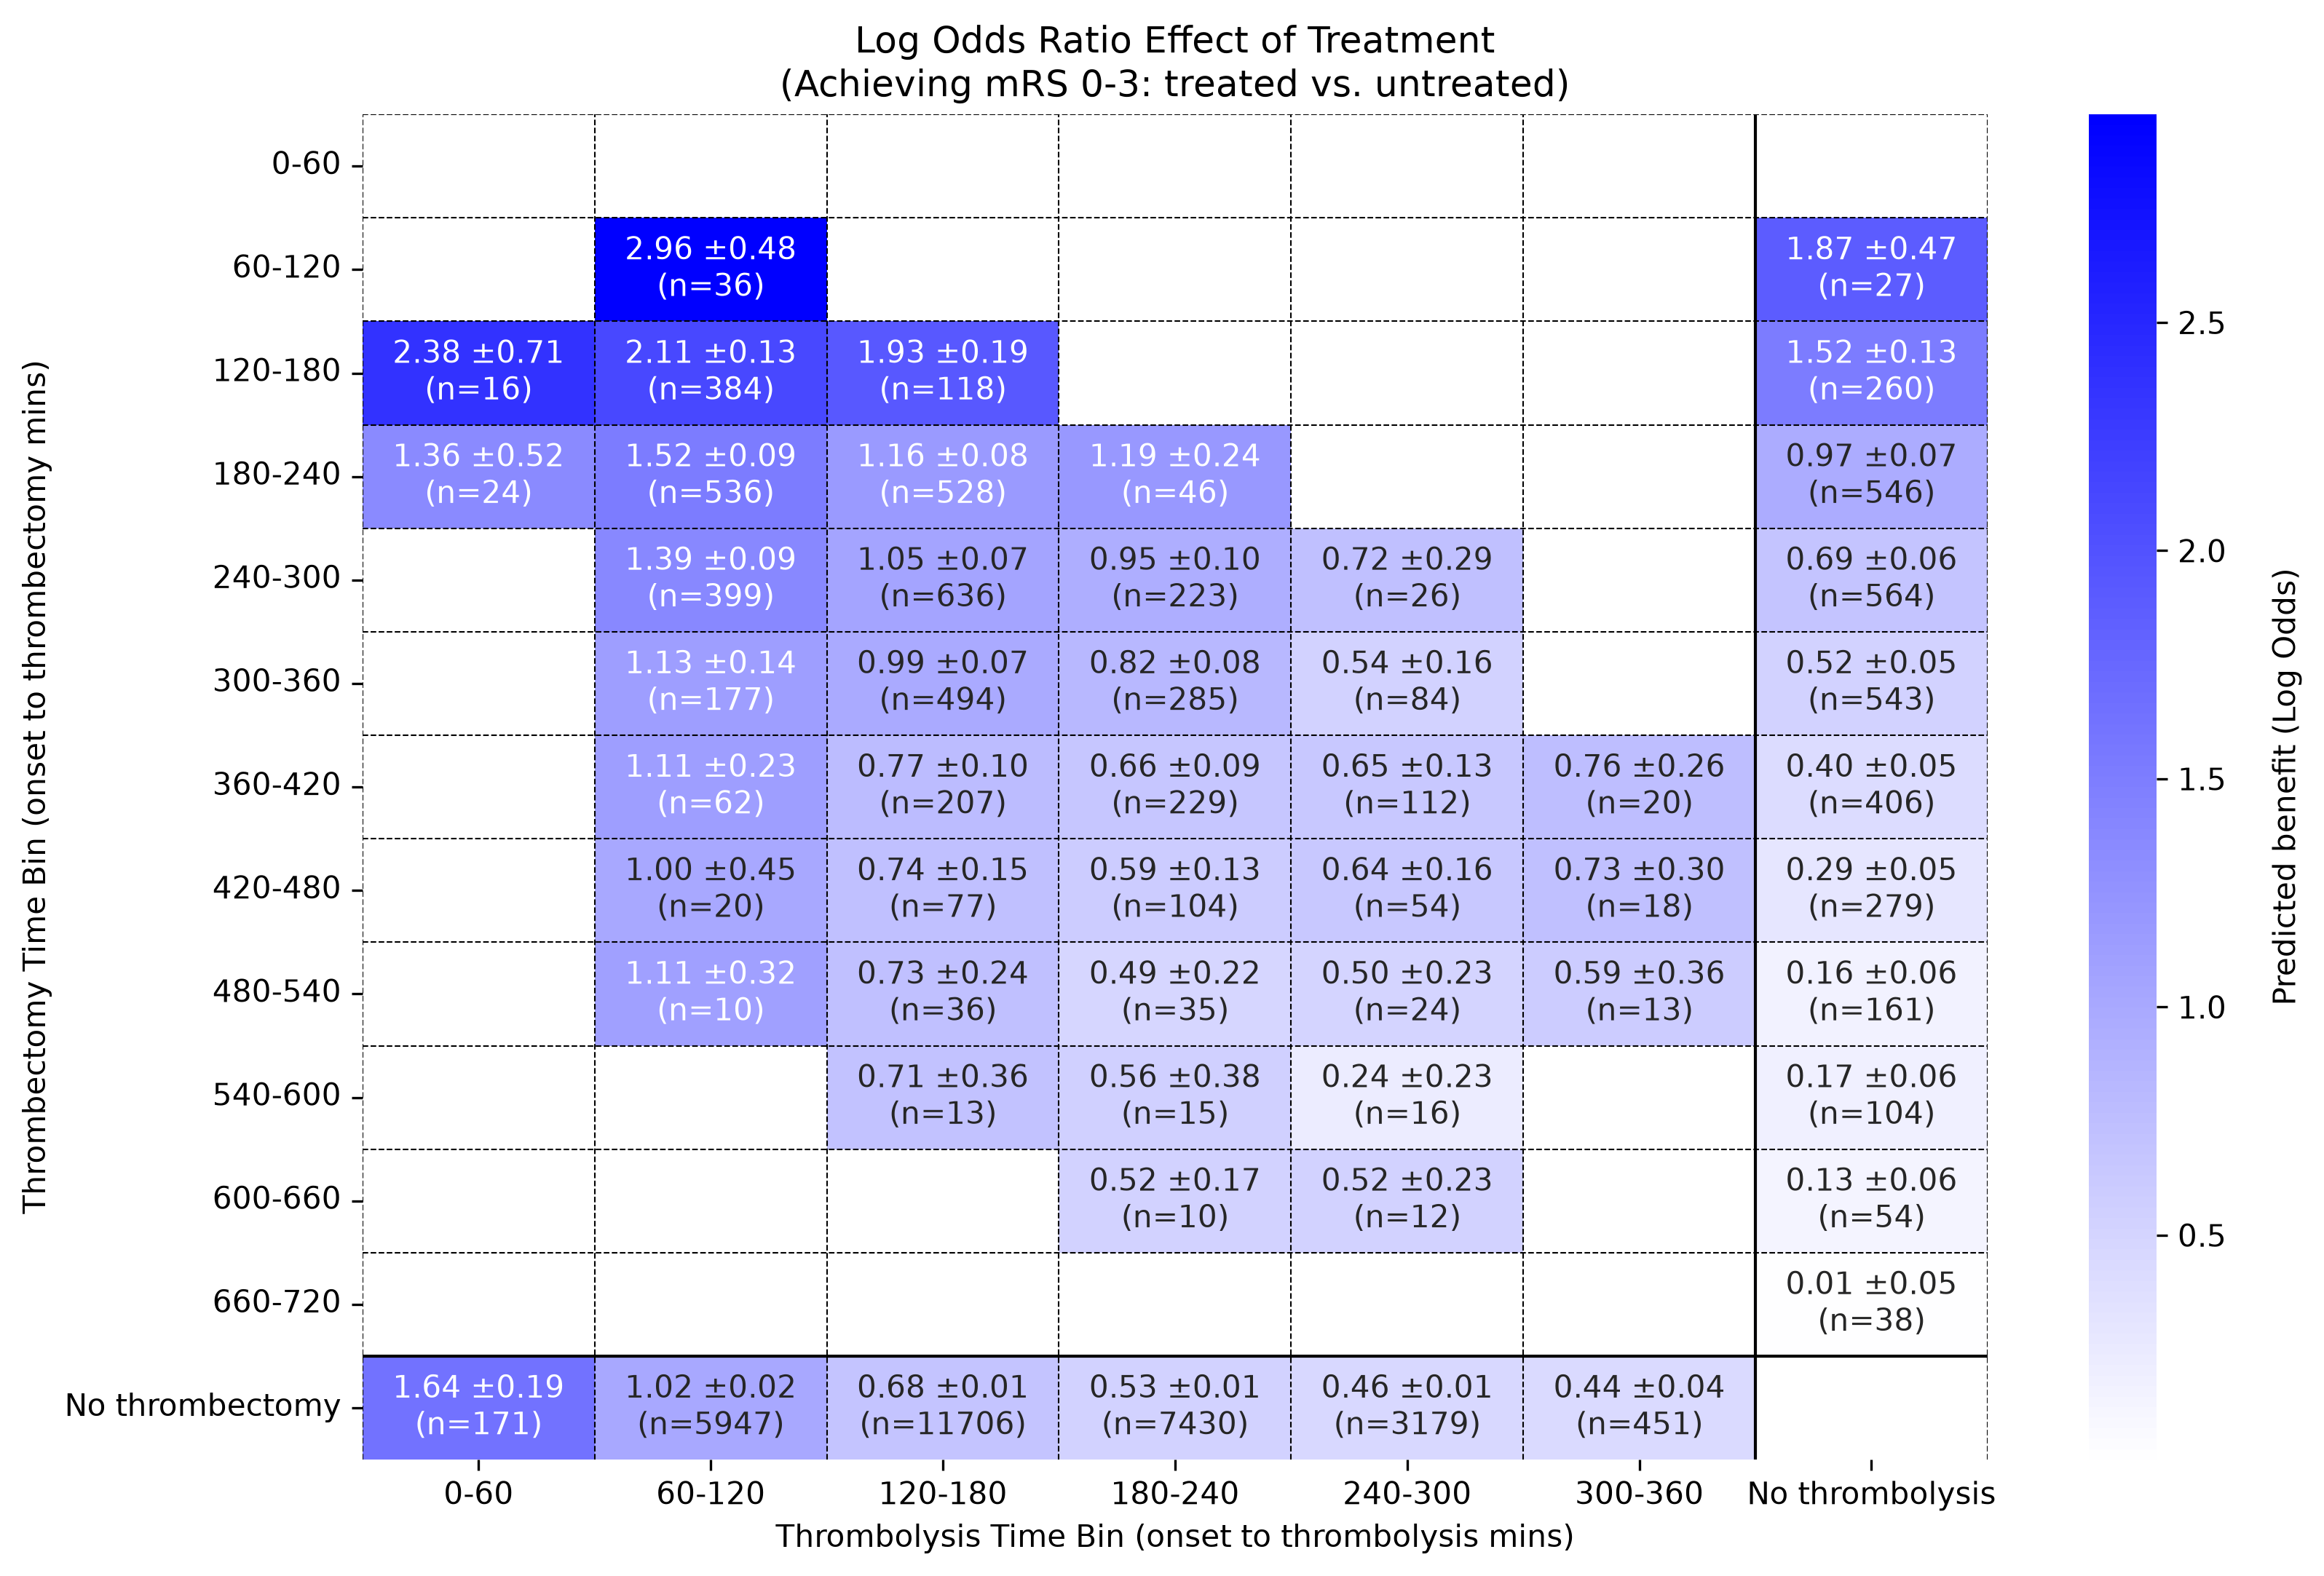
\includegraphics[width=\linewidth]{images/treatment_effects/thrombolysis_thrombectomy_heatmap_mrs_3.png}
        %\caption{}
    \end{subfigure}
    \hfill % Adds flexible horizontal spacing
    % Centre right image 
    \begin{subfigure}{0.48\textwidth}
        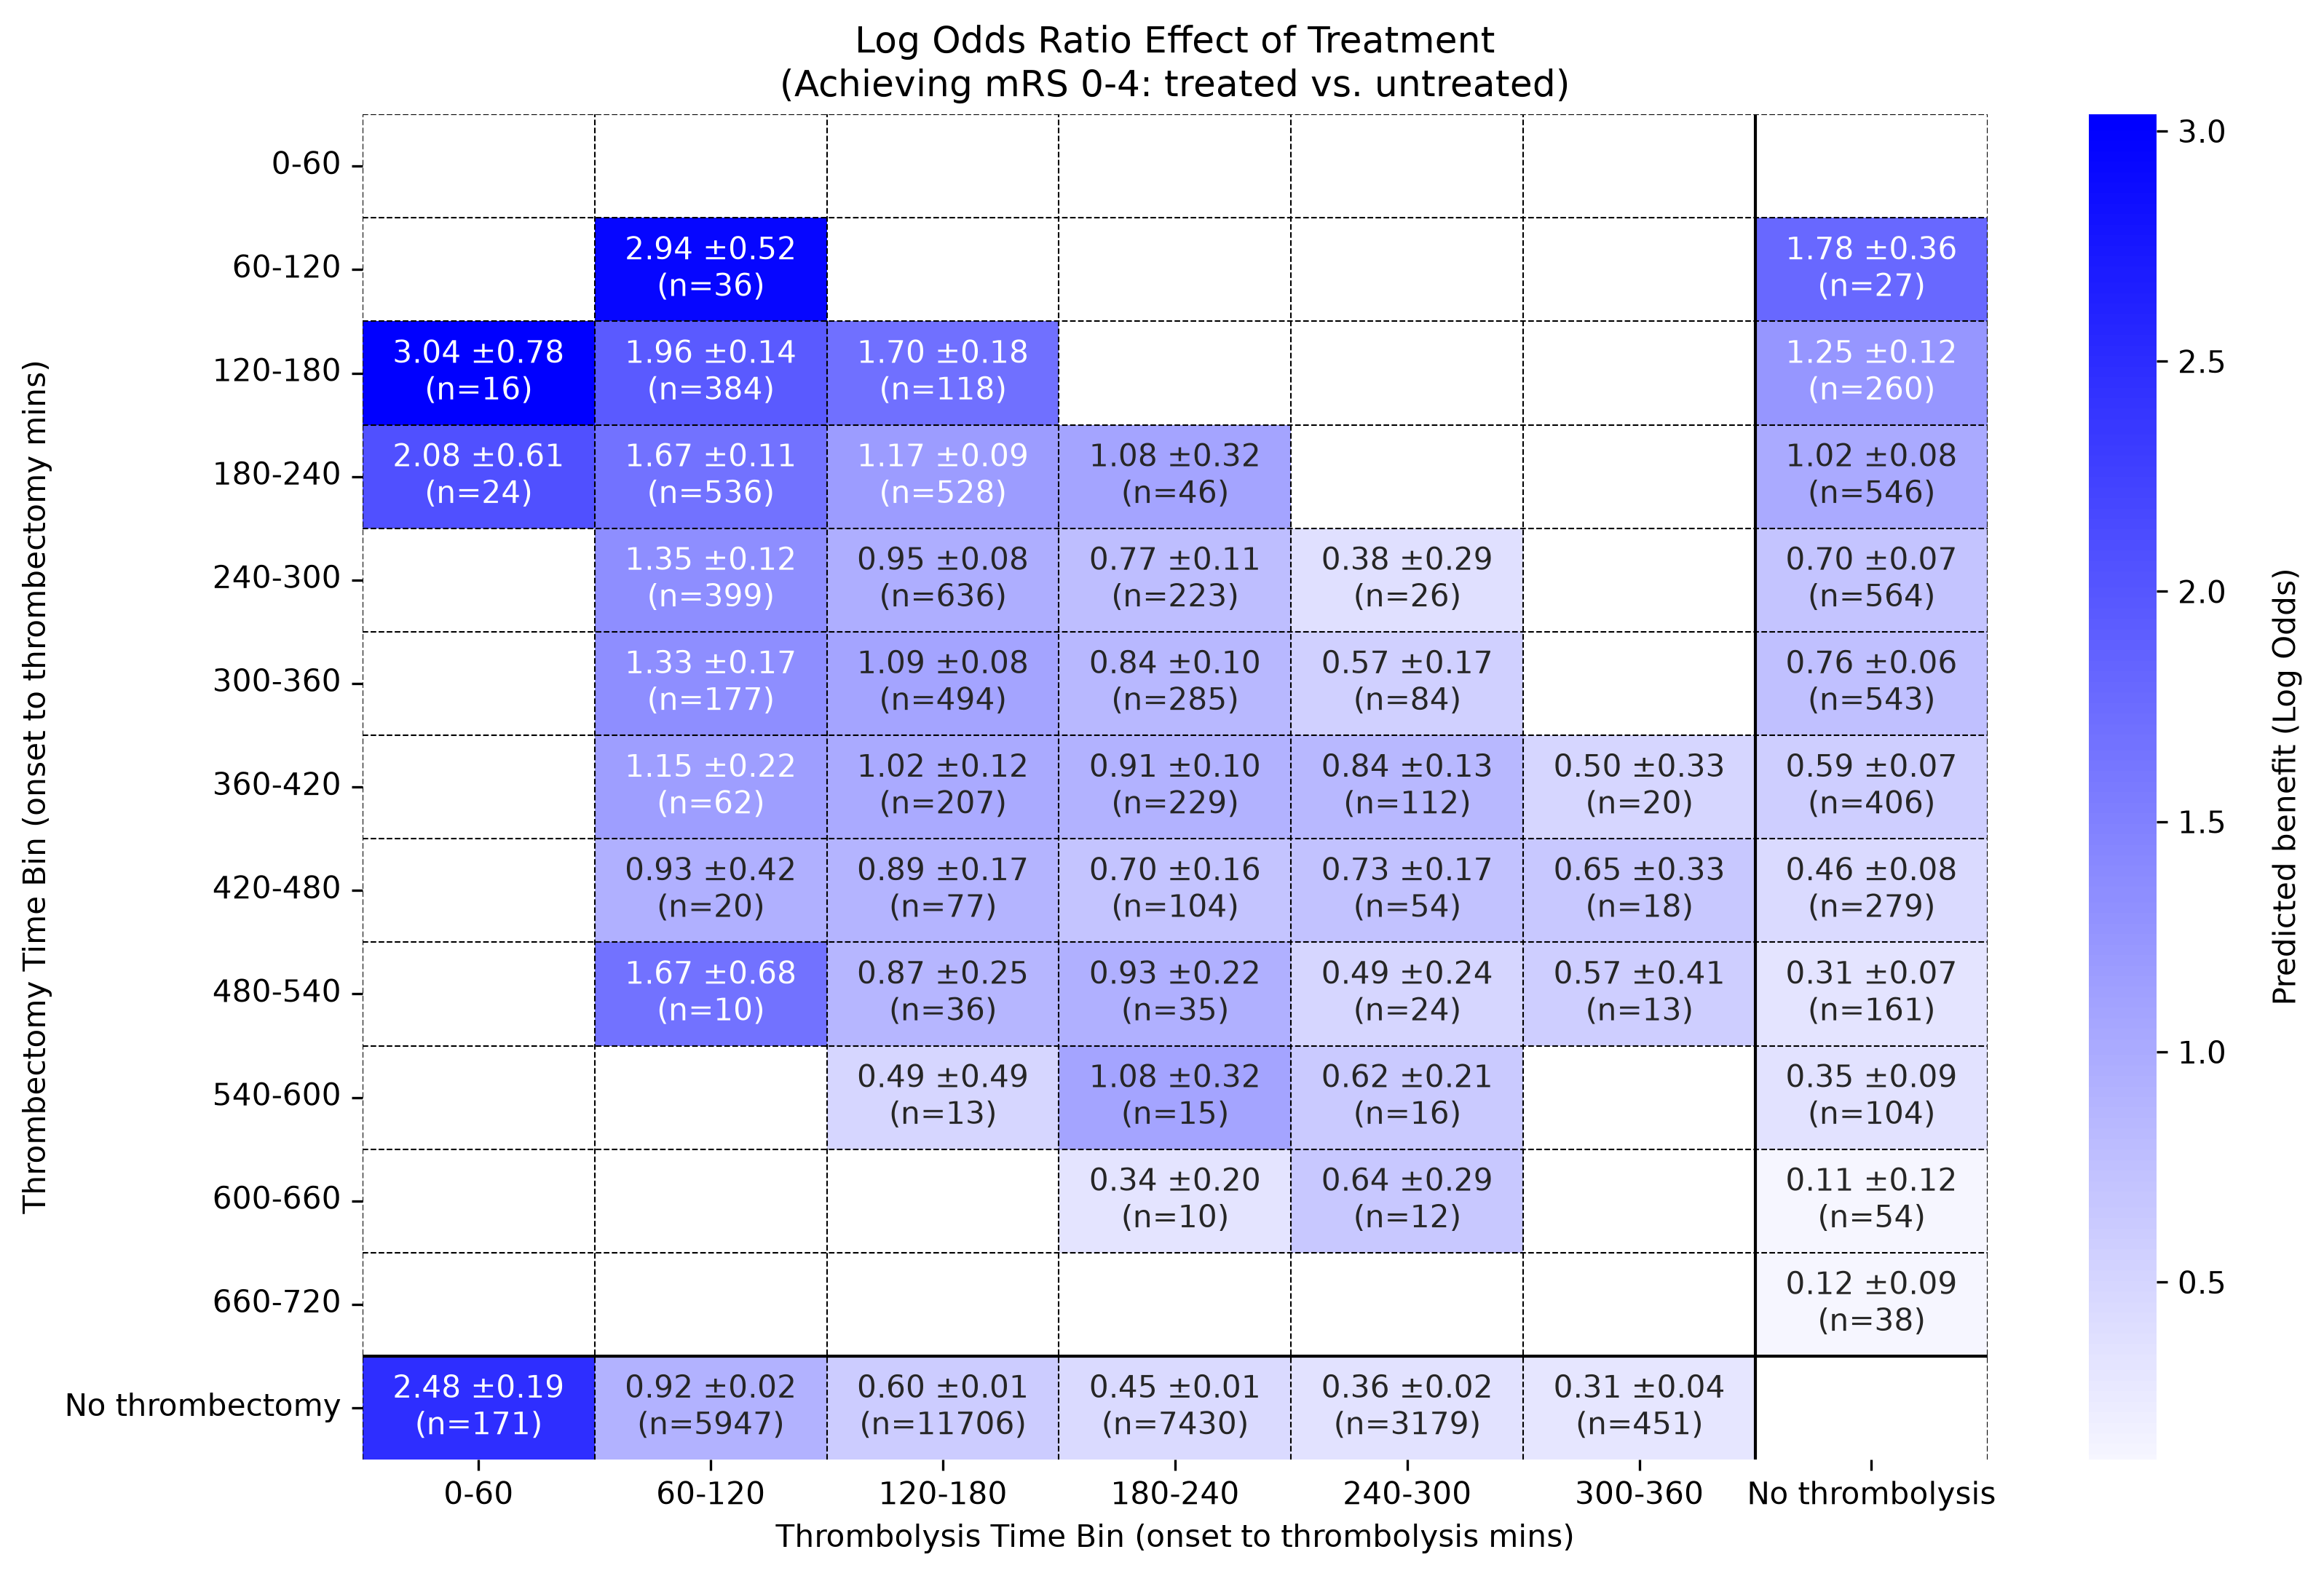
\includegraphics[width=\linewidth]{images/treatment_effects/thrombolysis_thrombectomy_heatmap_mrs_4.png}
        %\caption{}
    \end{subfigure}

    \vspace{0.5cm} % Optional vertical space between rows

    % Bottom image
    \begin{subfigure}{0.48\textwidth}
        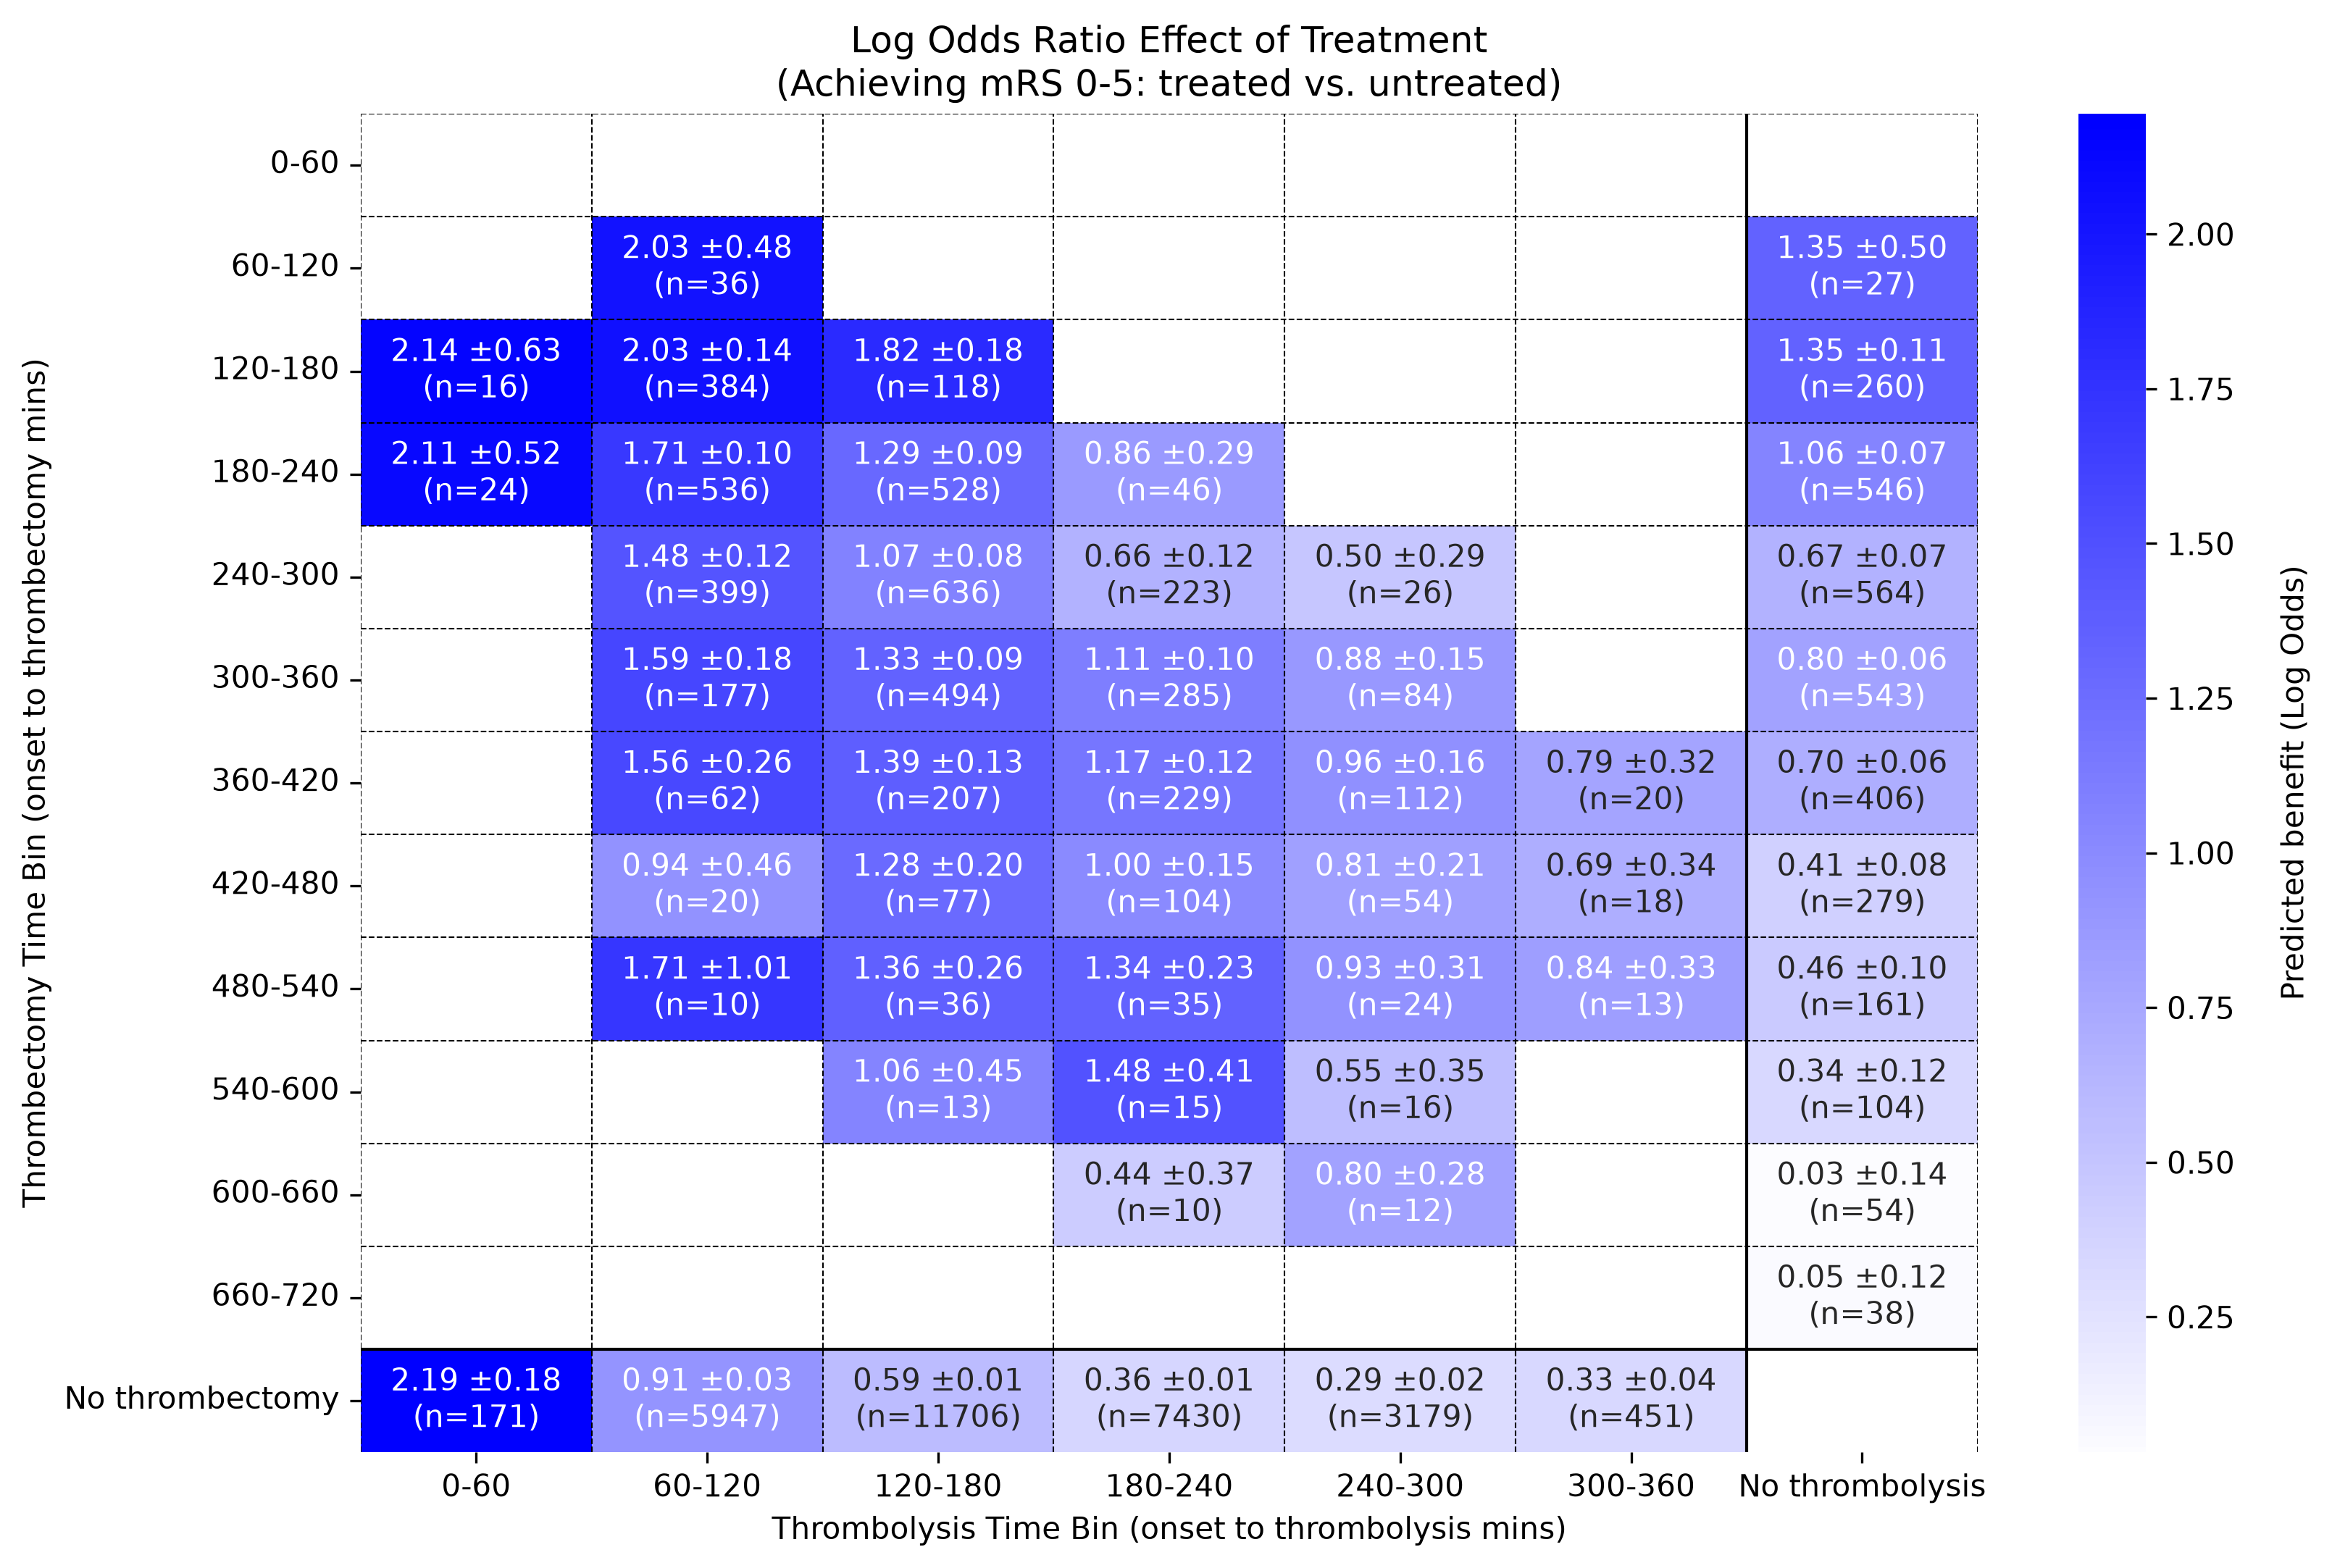
\includegraphics[width=\linewidth]{images/treatment_effects/thrombolysis_thrombectomy_heatmap_mrs_5}
        %\caption{}
    \end{subfigure}
    
    \caption{Predicted treatment benefit by thrombolysis and thrombectomy timing from the S-learner XGBoost model. Each panel shows a heatmap of the model-estimated effect of treatment on the log-odds of being discharged at each modified Rankin Scale (mRS) level, comparing treated with untreated patients across combinations of onset-to-thrombolysis and onset-to-thrombectomy time intervals. Each cell reports the mean predicted treatment benefit ± standard deviation, with the number of patients in parentheses. Blue shading denotes a positive predicted effect of treatment (increased log-odds of achieving each mRS level), whereas red shading denotes a negative predicted effect. The final row and column represent patients receiving thrombectomy without thrombolysis and thrombolysis without thrombectomy, respectively; blank cells indicate treatment-timing combinations with fewer than 10 observations in the data}
    \label{fig:s_learner_heatmap_log odds}
\end{figure}



%%%%%%%%%%%%%%%%%%%%%%%%%%%%%%%%%%%%%%%%%%

Figure \ref{fig:s_learner_time_thrombolysis} shows a scatter plot, with regression line, of the estimated benefit of thrombolysis (log odds ratio, treated vs untreated), by time after onset, in achieving each mRS threshold. This model used actual onset-to-treatment times for thrombolysis, and includes only patients who received thrombolysis without thrombectomy. Each point represents one patient. The fitted line shows the average decline in benefit with increasing time to treatment: extrapolating it back to the time of onset gives the maximum expected benefit, and the time at which it crosses zero gives the estimated time beyond which no benefit would be expected.

\begin{figure}[htbp]
    \centering
    
    % Top left
    \begin{subfigure}{0.38\textwidth}
        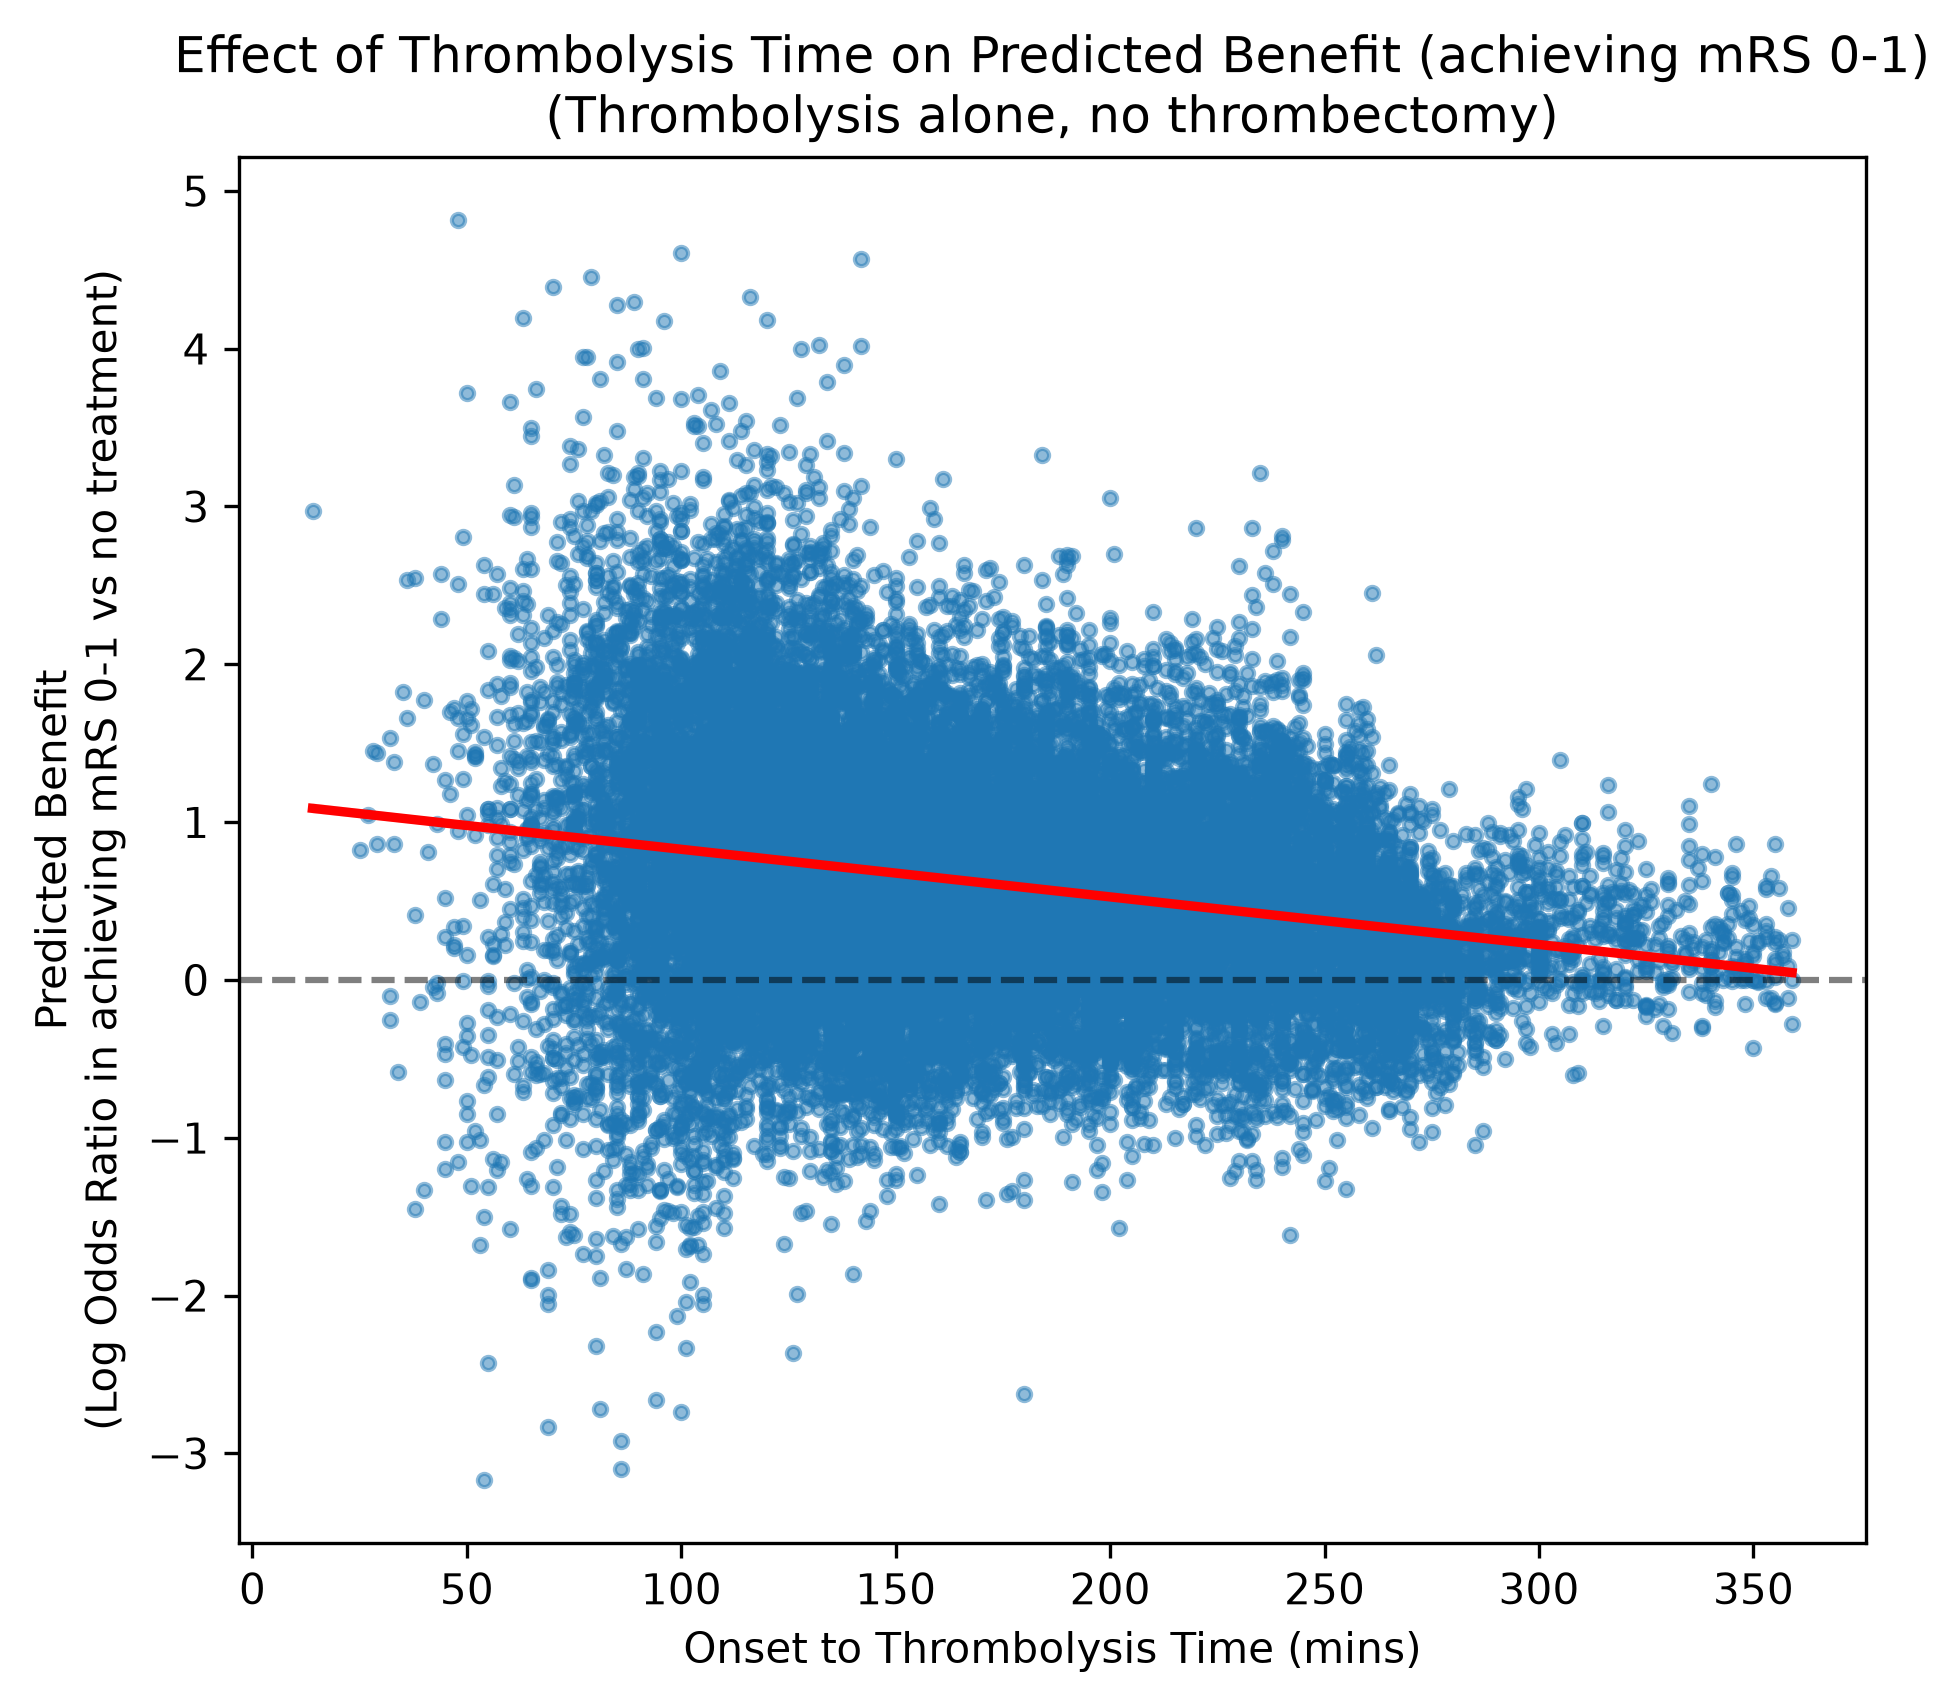
\includegraphics[width=\linewidth]{images/treatment_effects/thrombolysis_alone_time_effect_mrs_1.png}
        %\caption{}
    \end{subfigure}
    %\hfill % Adds flexible horizontal spacing
    % top right image 
    \begin{subfigure}{0.38\textwidth}
        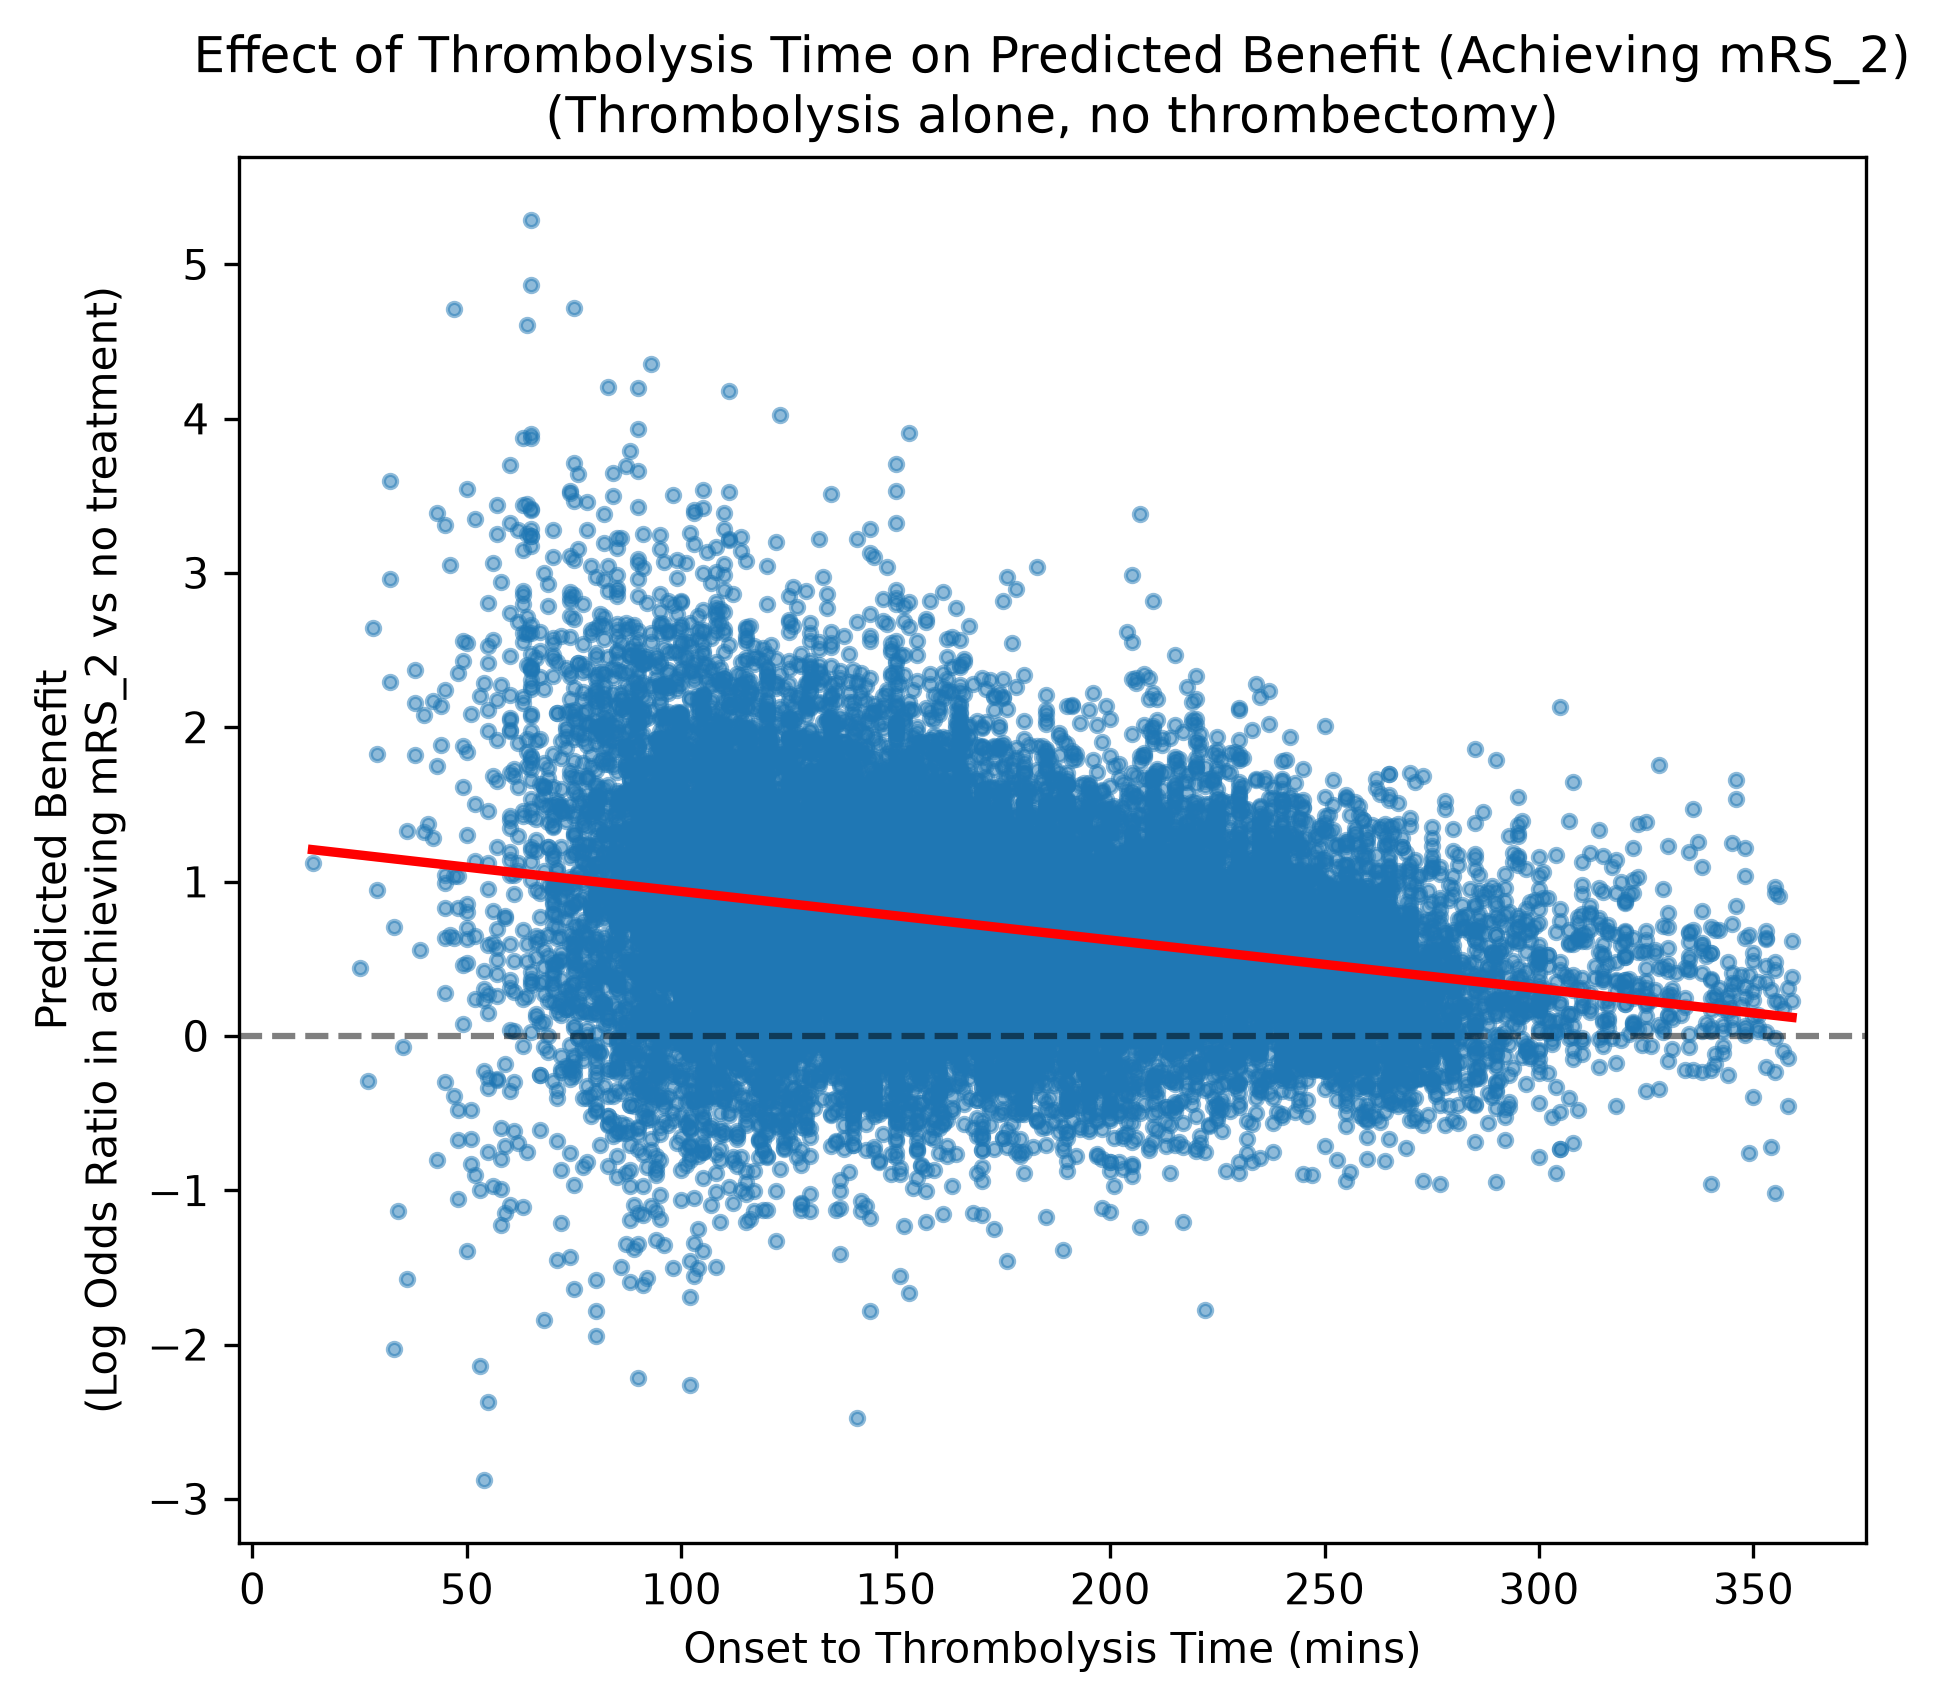
\includegraphics[width=\linewidth]{images/treatment_effects/thrombolysis_alone_time_effect_mrs_2.png}
        %\caption{}
    \end{subfigure}

    \vspace{0.2cm} % Optional vertical space between rows

    % Center left image
    \begin{subfigure}{0.38\textwidth}
        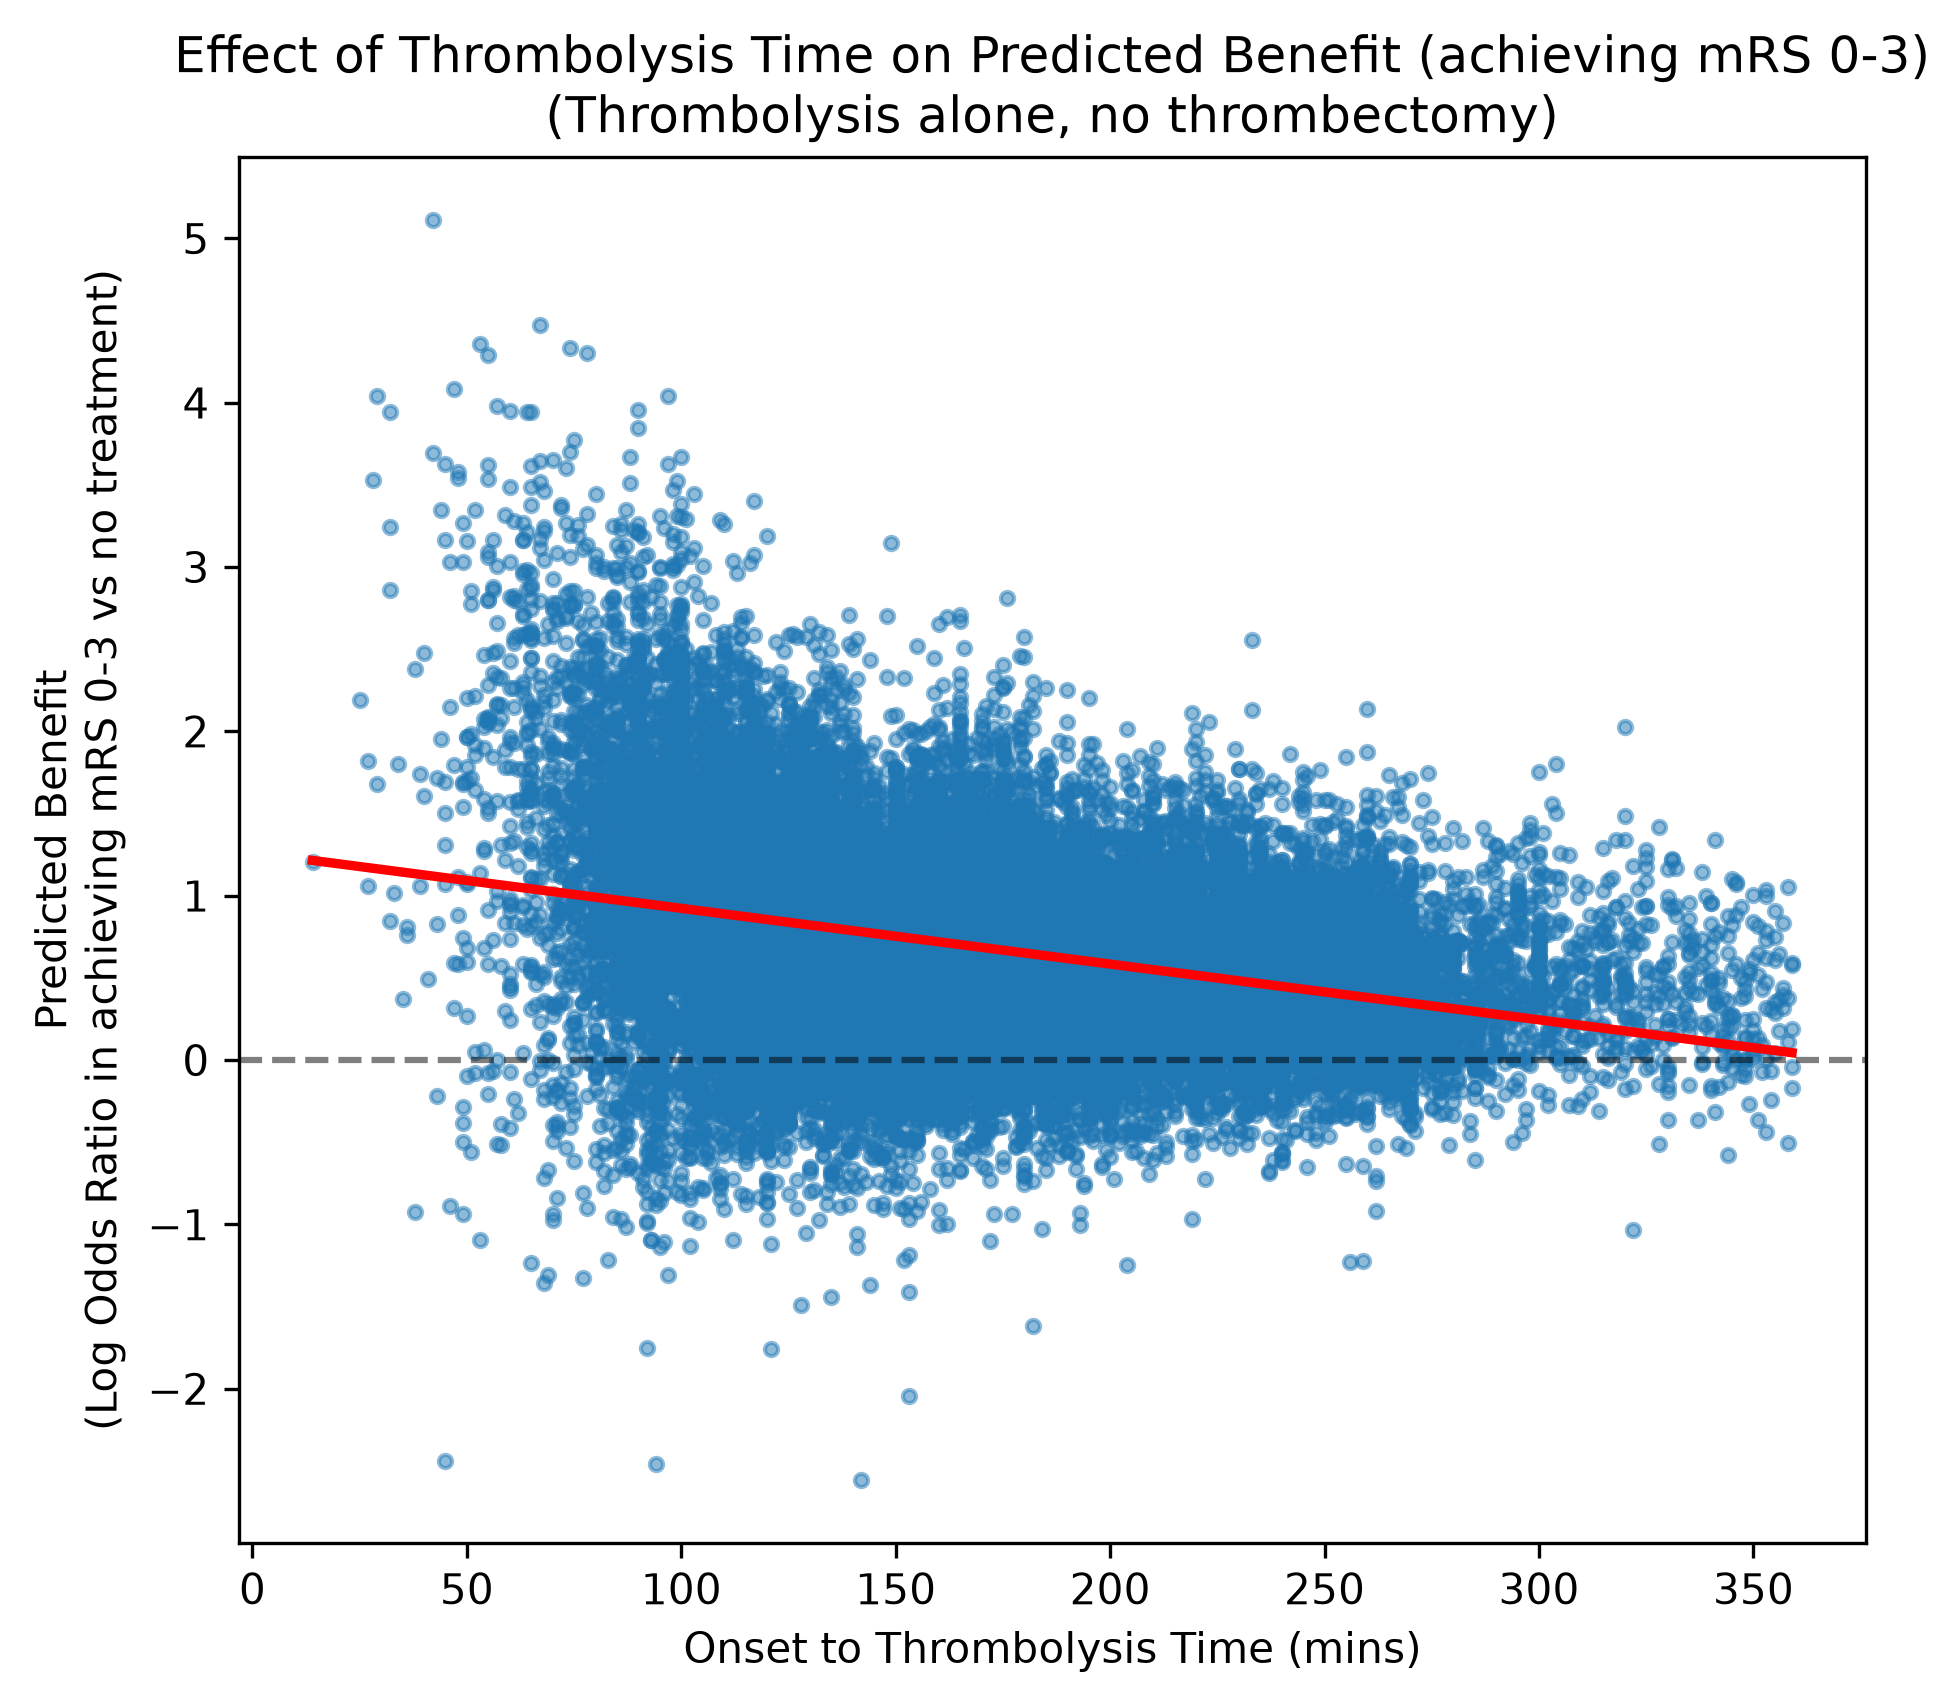
\includegraphics[width=\linewidth]{images/treatment_effects/thrombolysis_alone_time_effect_mrs_3.png}
        %\caption{}
    \end{subfigure}
    %\hfill % Adds flexible horizontal spacing
    % Centre right image 
    \begin{subfigure}{0.38\textwidth}
        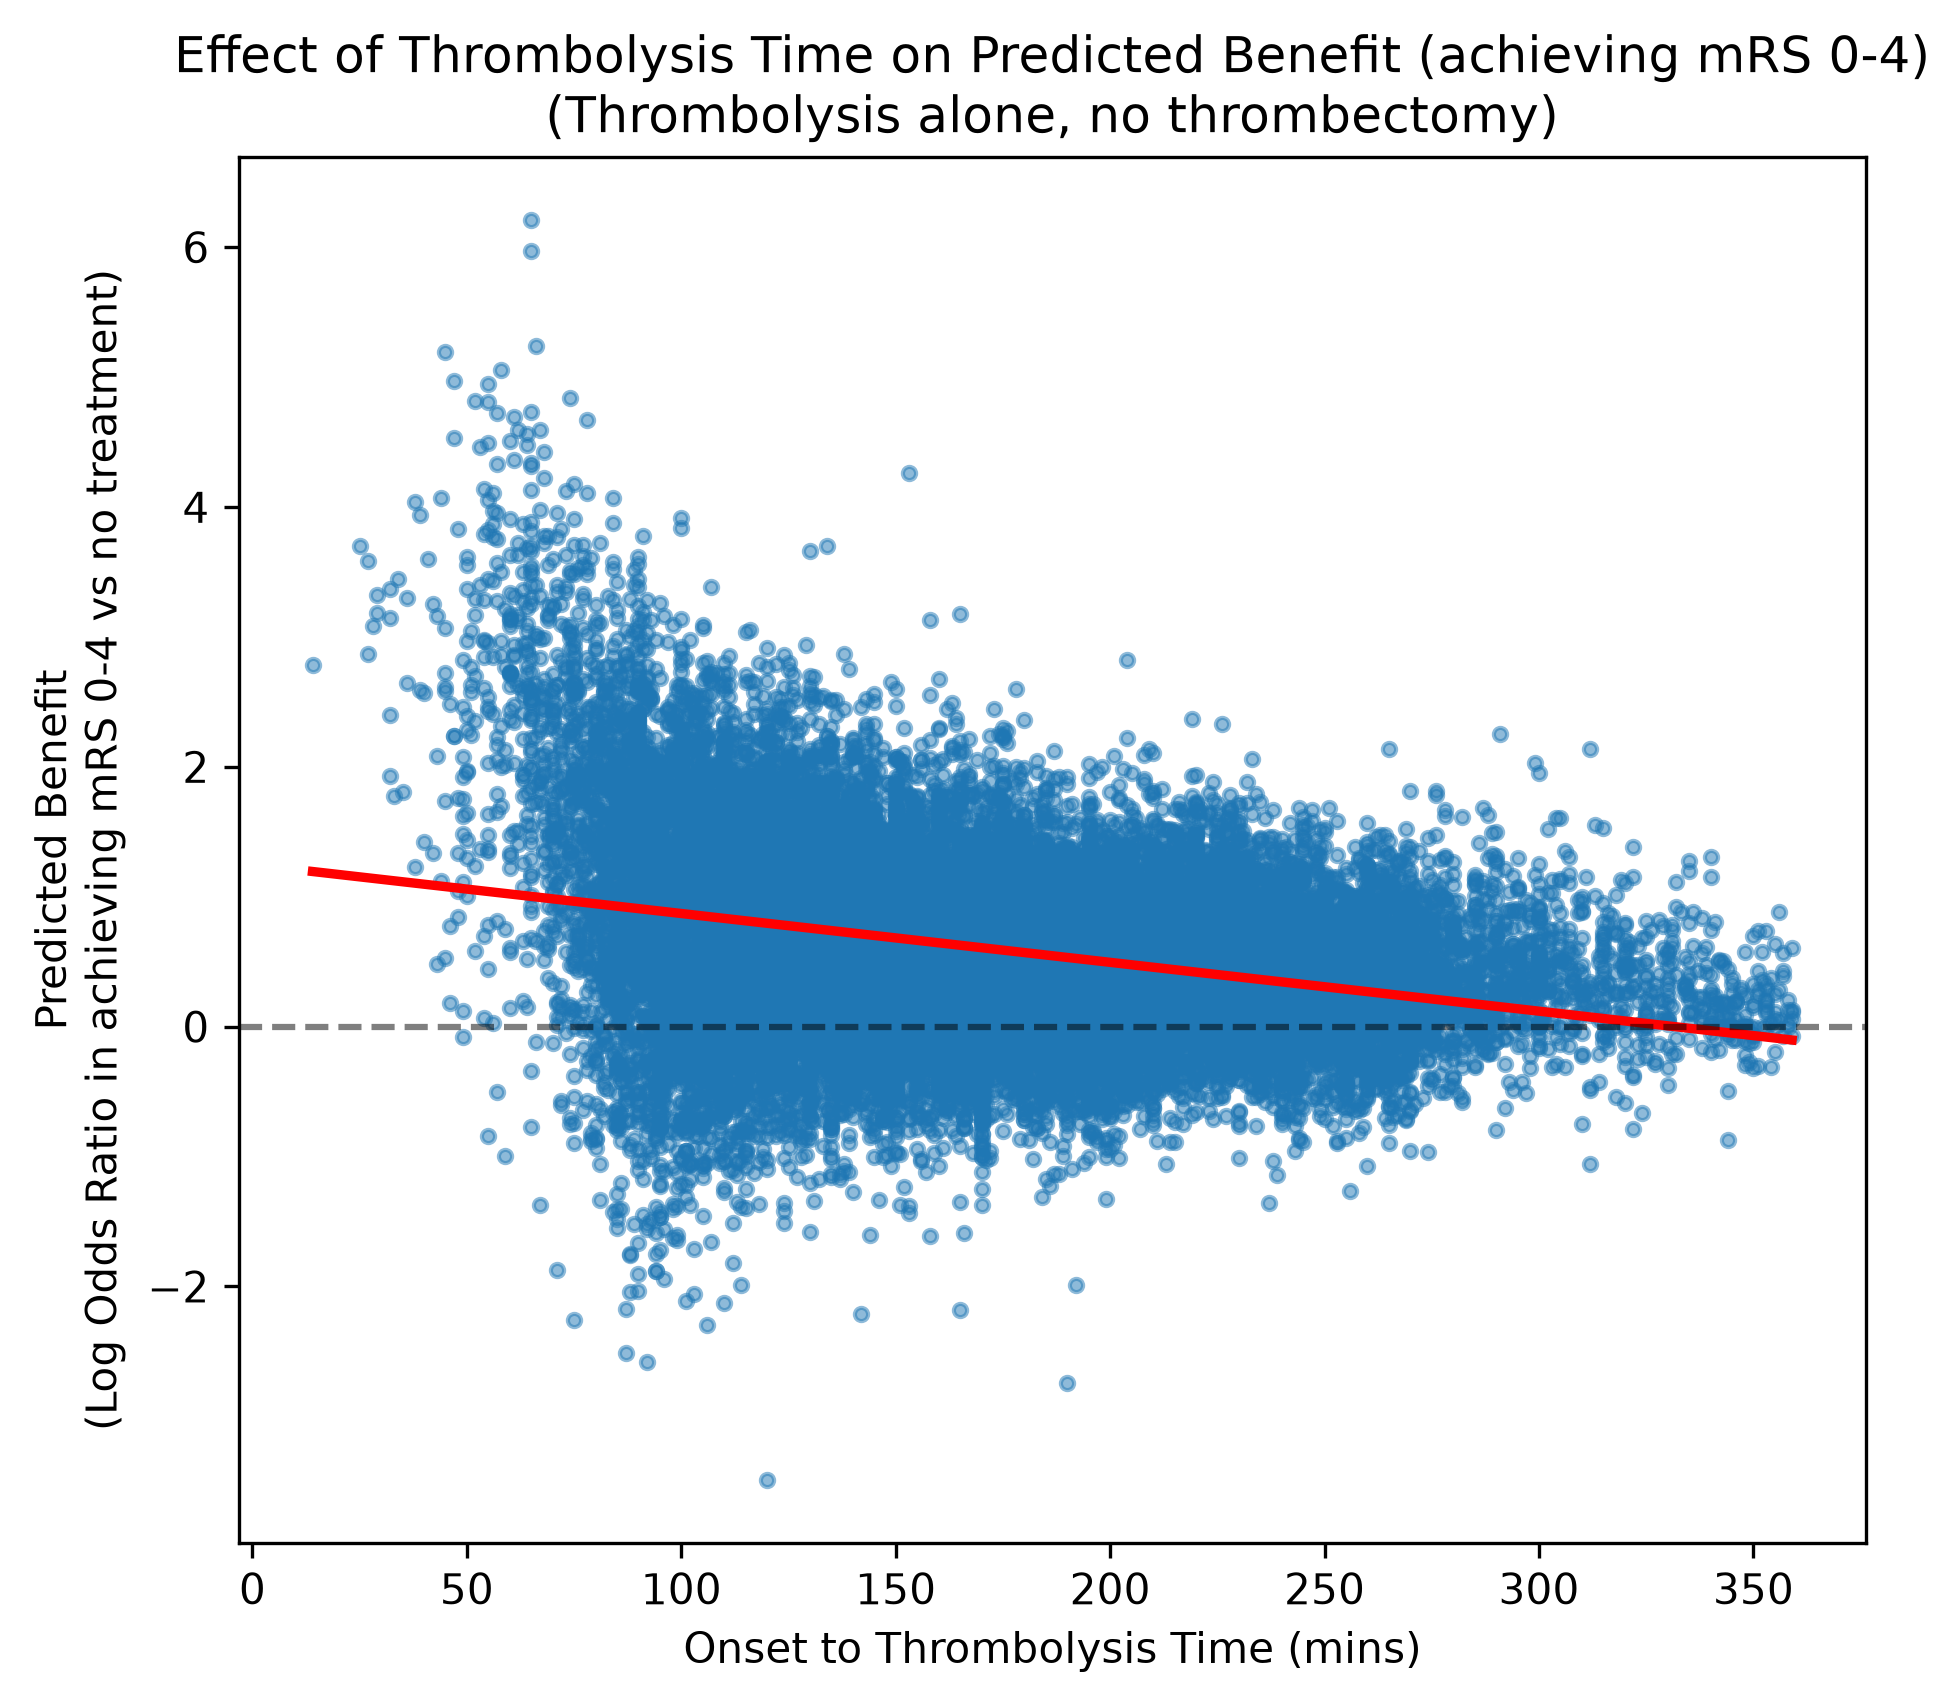
\includegraphics[width=\linewidth]{images/treatment_effects/thrombolysis_alone_time_effect_mrs_4.png}
        %\caption{}
    \end{subfigure}

    \vspace{0.2cm} % Optional vertical space between rows

    % Bottom image
    \begin{subfigure}{0.38\textwidth}
        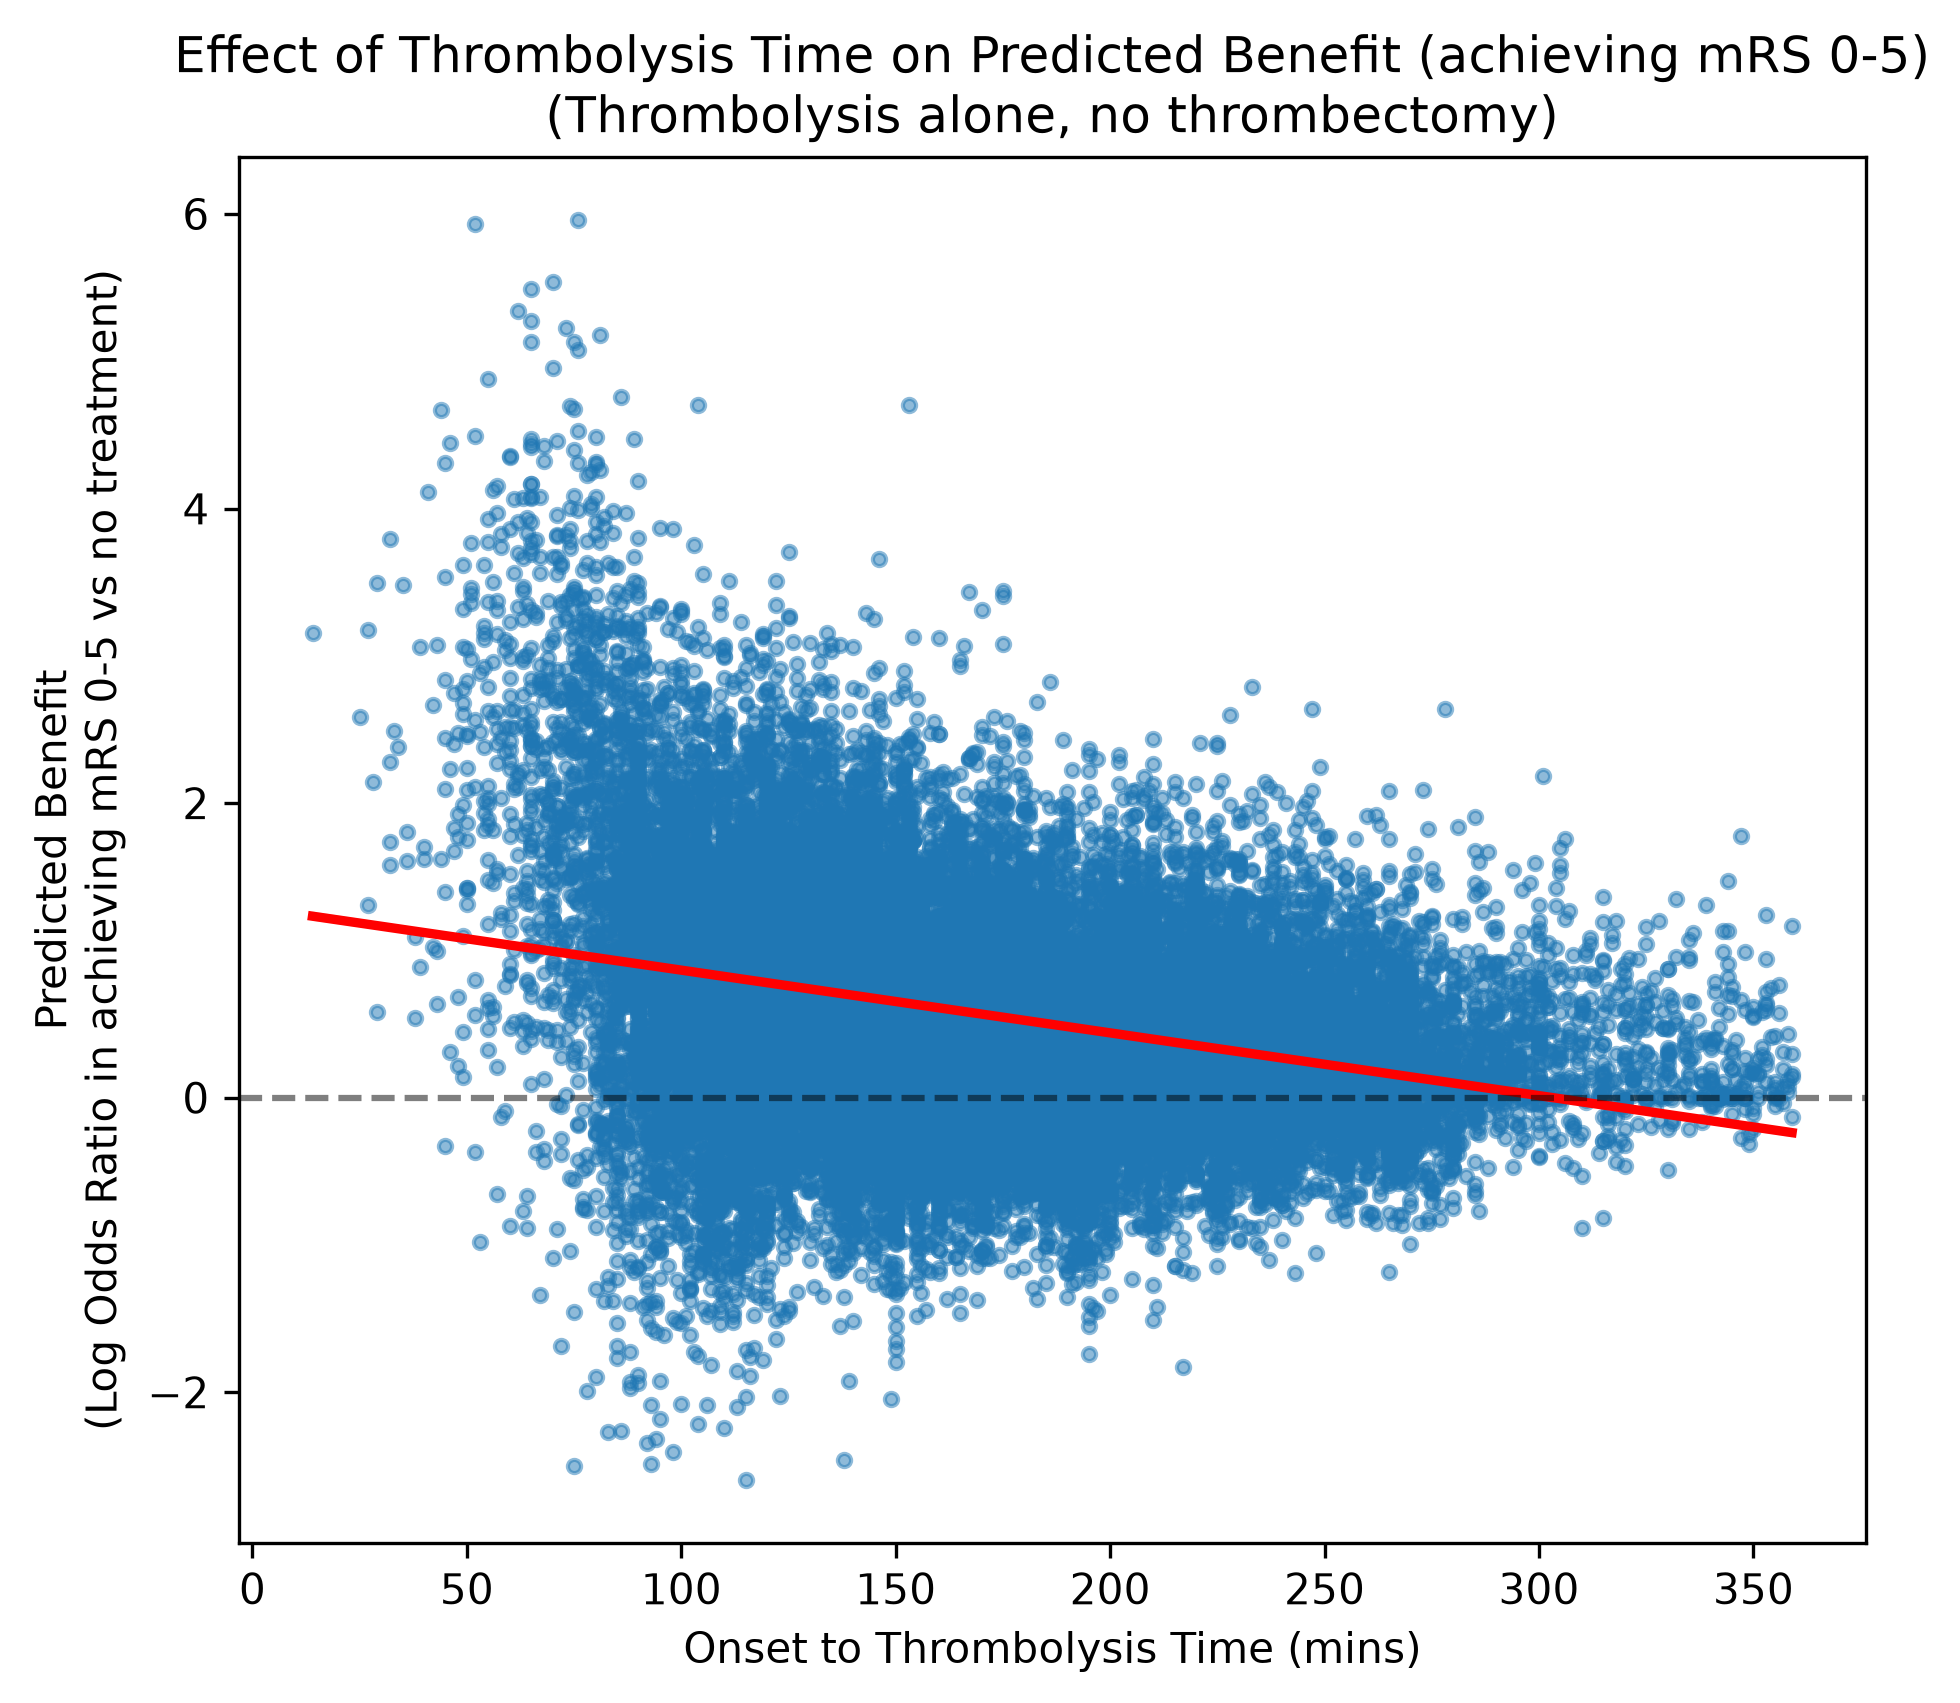
\includegraphics[width=\linewidth]{images/treatment_effects/thrombolysis_alone_time_effect_mrs_5}
        %\caption{}
    \end{subfigure}
    
    \caption{Association between onset-to-thrombolysis time and individualised predicted benefit of thrombolysis alone, estimated using the S-learner XGBoost model. Each panel shows the predicted improvement in the odds of a good outcome (discharge at or below the specified modified Rankin Scale (mRS) threshold, or no worse than the pre-stroke mRS). Analyses are restricted to patients receiving intravenous thrombolysis without mechanical thrombectomy; each point represents an individual patient. The vertical axis shows the model-estimated treatment benefit on the log-odds scale, relative to the counterfactual prediction under no treatment. The red line denotes the fitted linear trend, illustrating the decline in predicted benefit with increasing onset-to-thrombolysis time. The dashed horizontal line indicates no predicted treatment benefit (log-odds ratio = 0); values above and below this line indicate predicted benefit and harm, respectively.}
    \label{fig:s_learner_time_thrombolysis}
\end{figure}


%%%%%%%%%%%%%%%%%%%%%%%%%%%%%%%%%%%%%%%%%%

Figure \ref{fig:s_learner_time_thrombectomy} shows a scatter plot, with regression line, of the estimated benefit of thrombectomy (log odds ratio, treated vs untreated), by time after onset, in achieving each mRS threshold. This model used actual onset-to-treatment times for thrombectomy, and includes only patients who received thrombectomy without thrombolysis. As for thrombolysis, each point represents one patient, and the fitted line summarises how benefit declines with time to treatment.


\begin{figure}[htbp]
    \centering
    
    % Top left
    \begin{subfigure}{0.38\textwidth}
        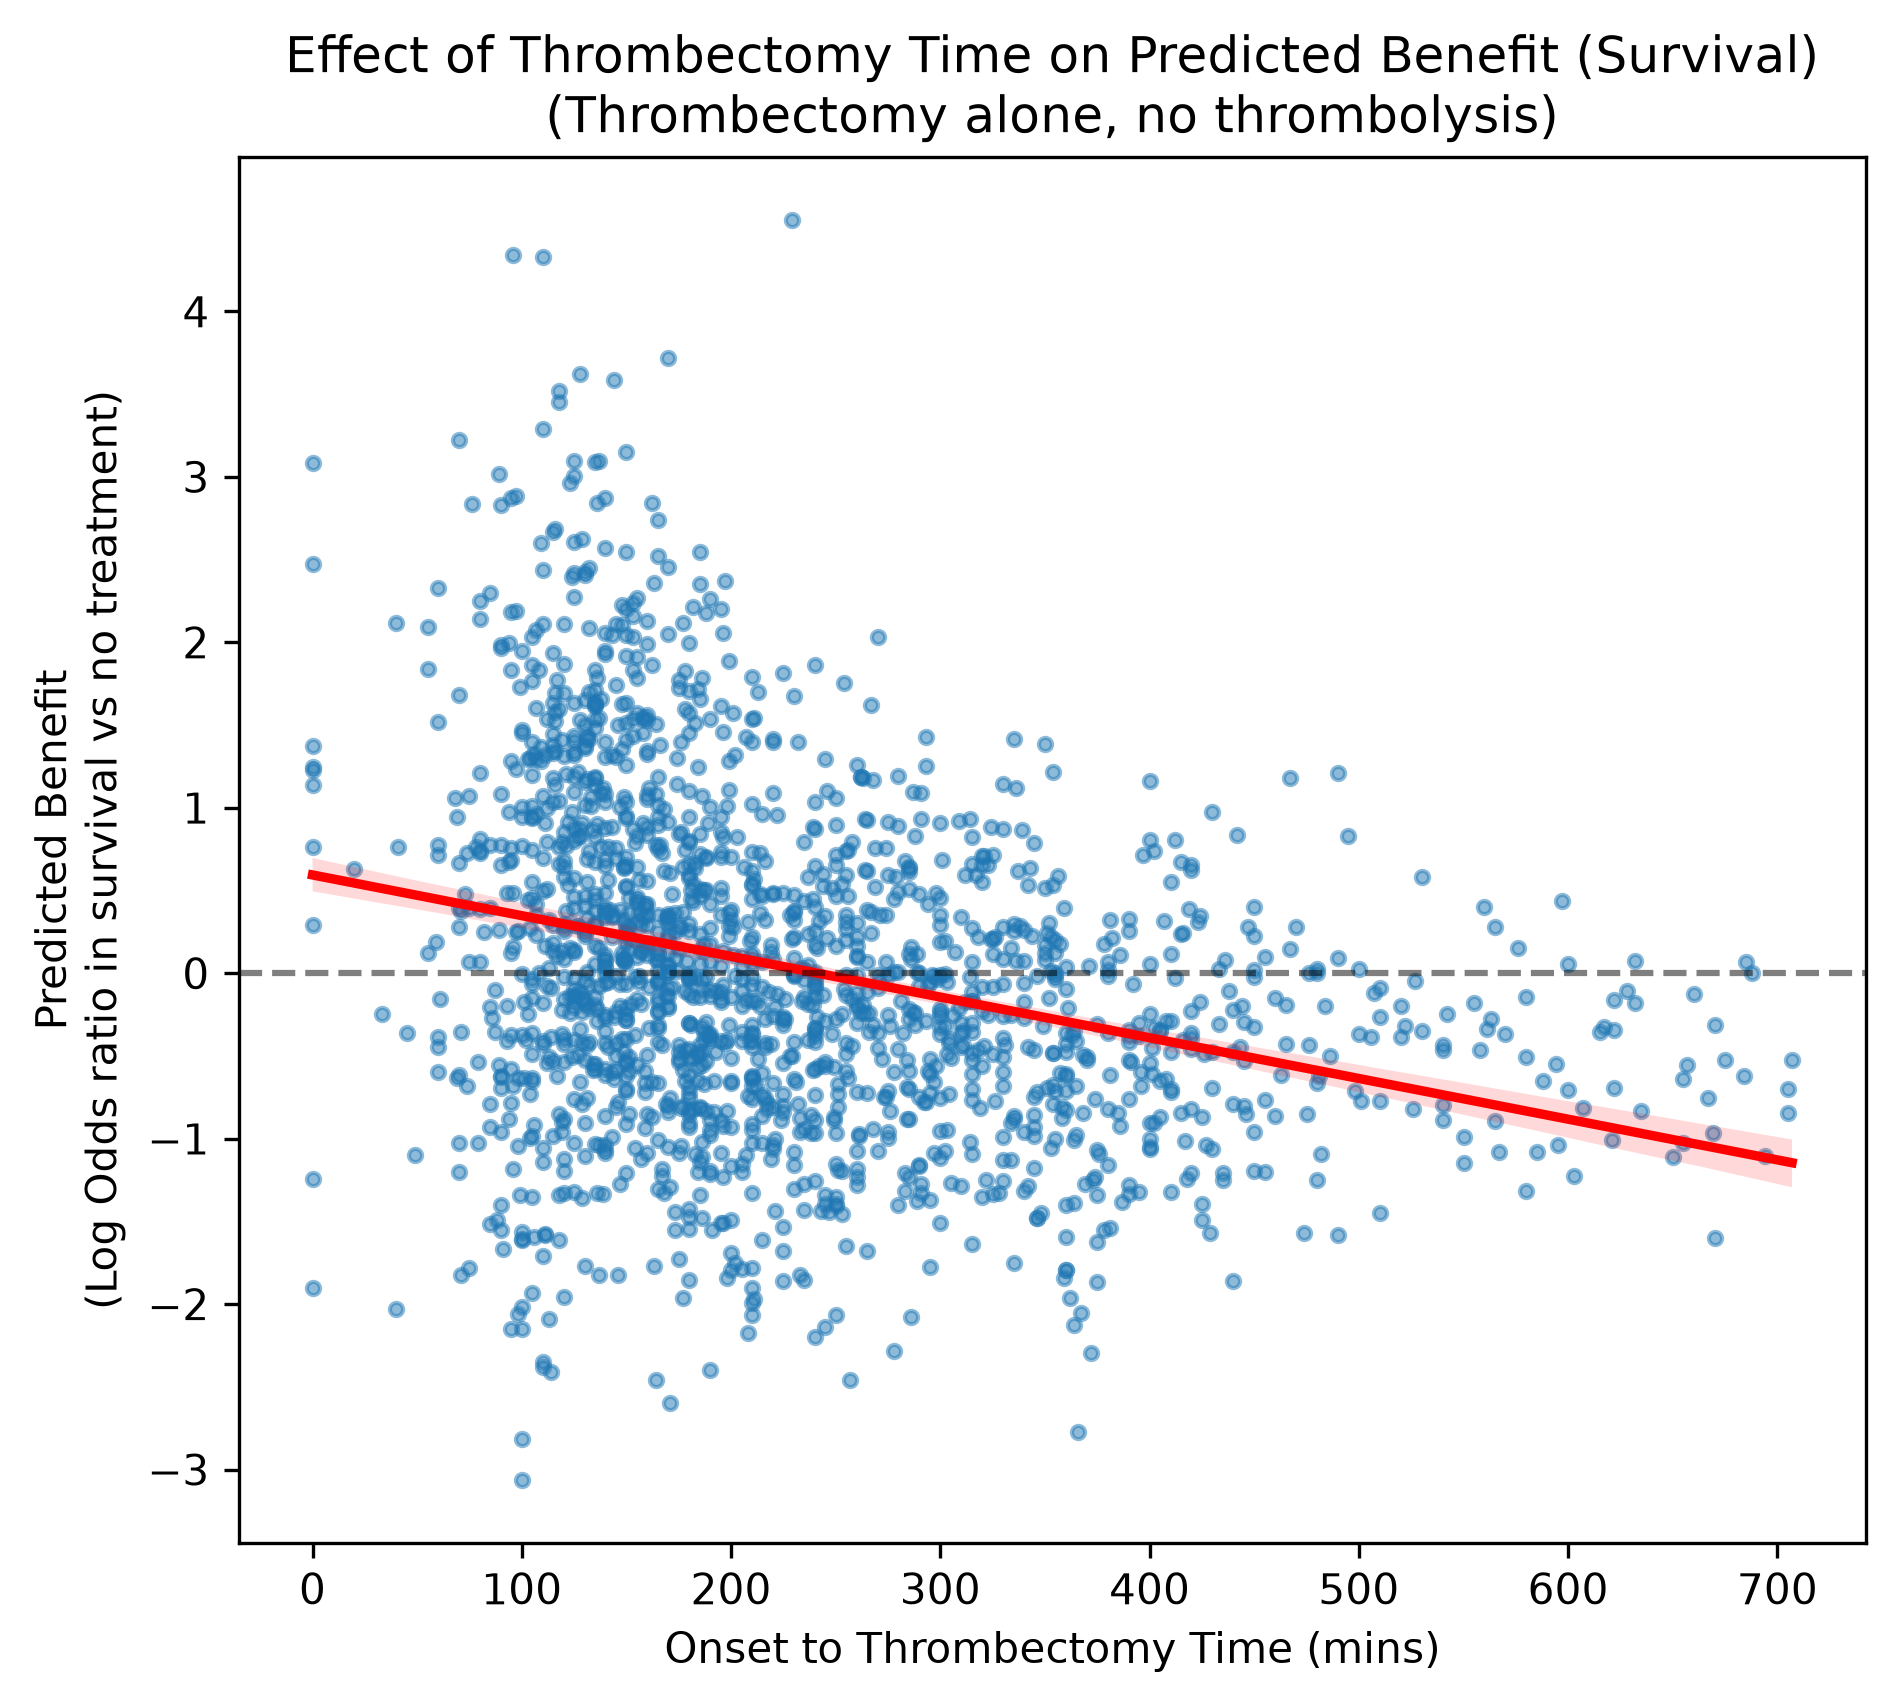
\includegraphics[width=\linewidth]{images/treatment_effects/thrombectomy_alone_time_effect_mrs_1.png}
        %\caption{}
    \end{subfigure}
    %\hfill % Adds flexible horizontal spacing
    % top right image 
    \begin{subfigure}{0.38\textwidth}
        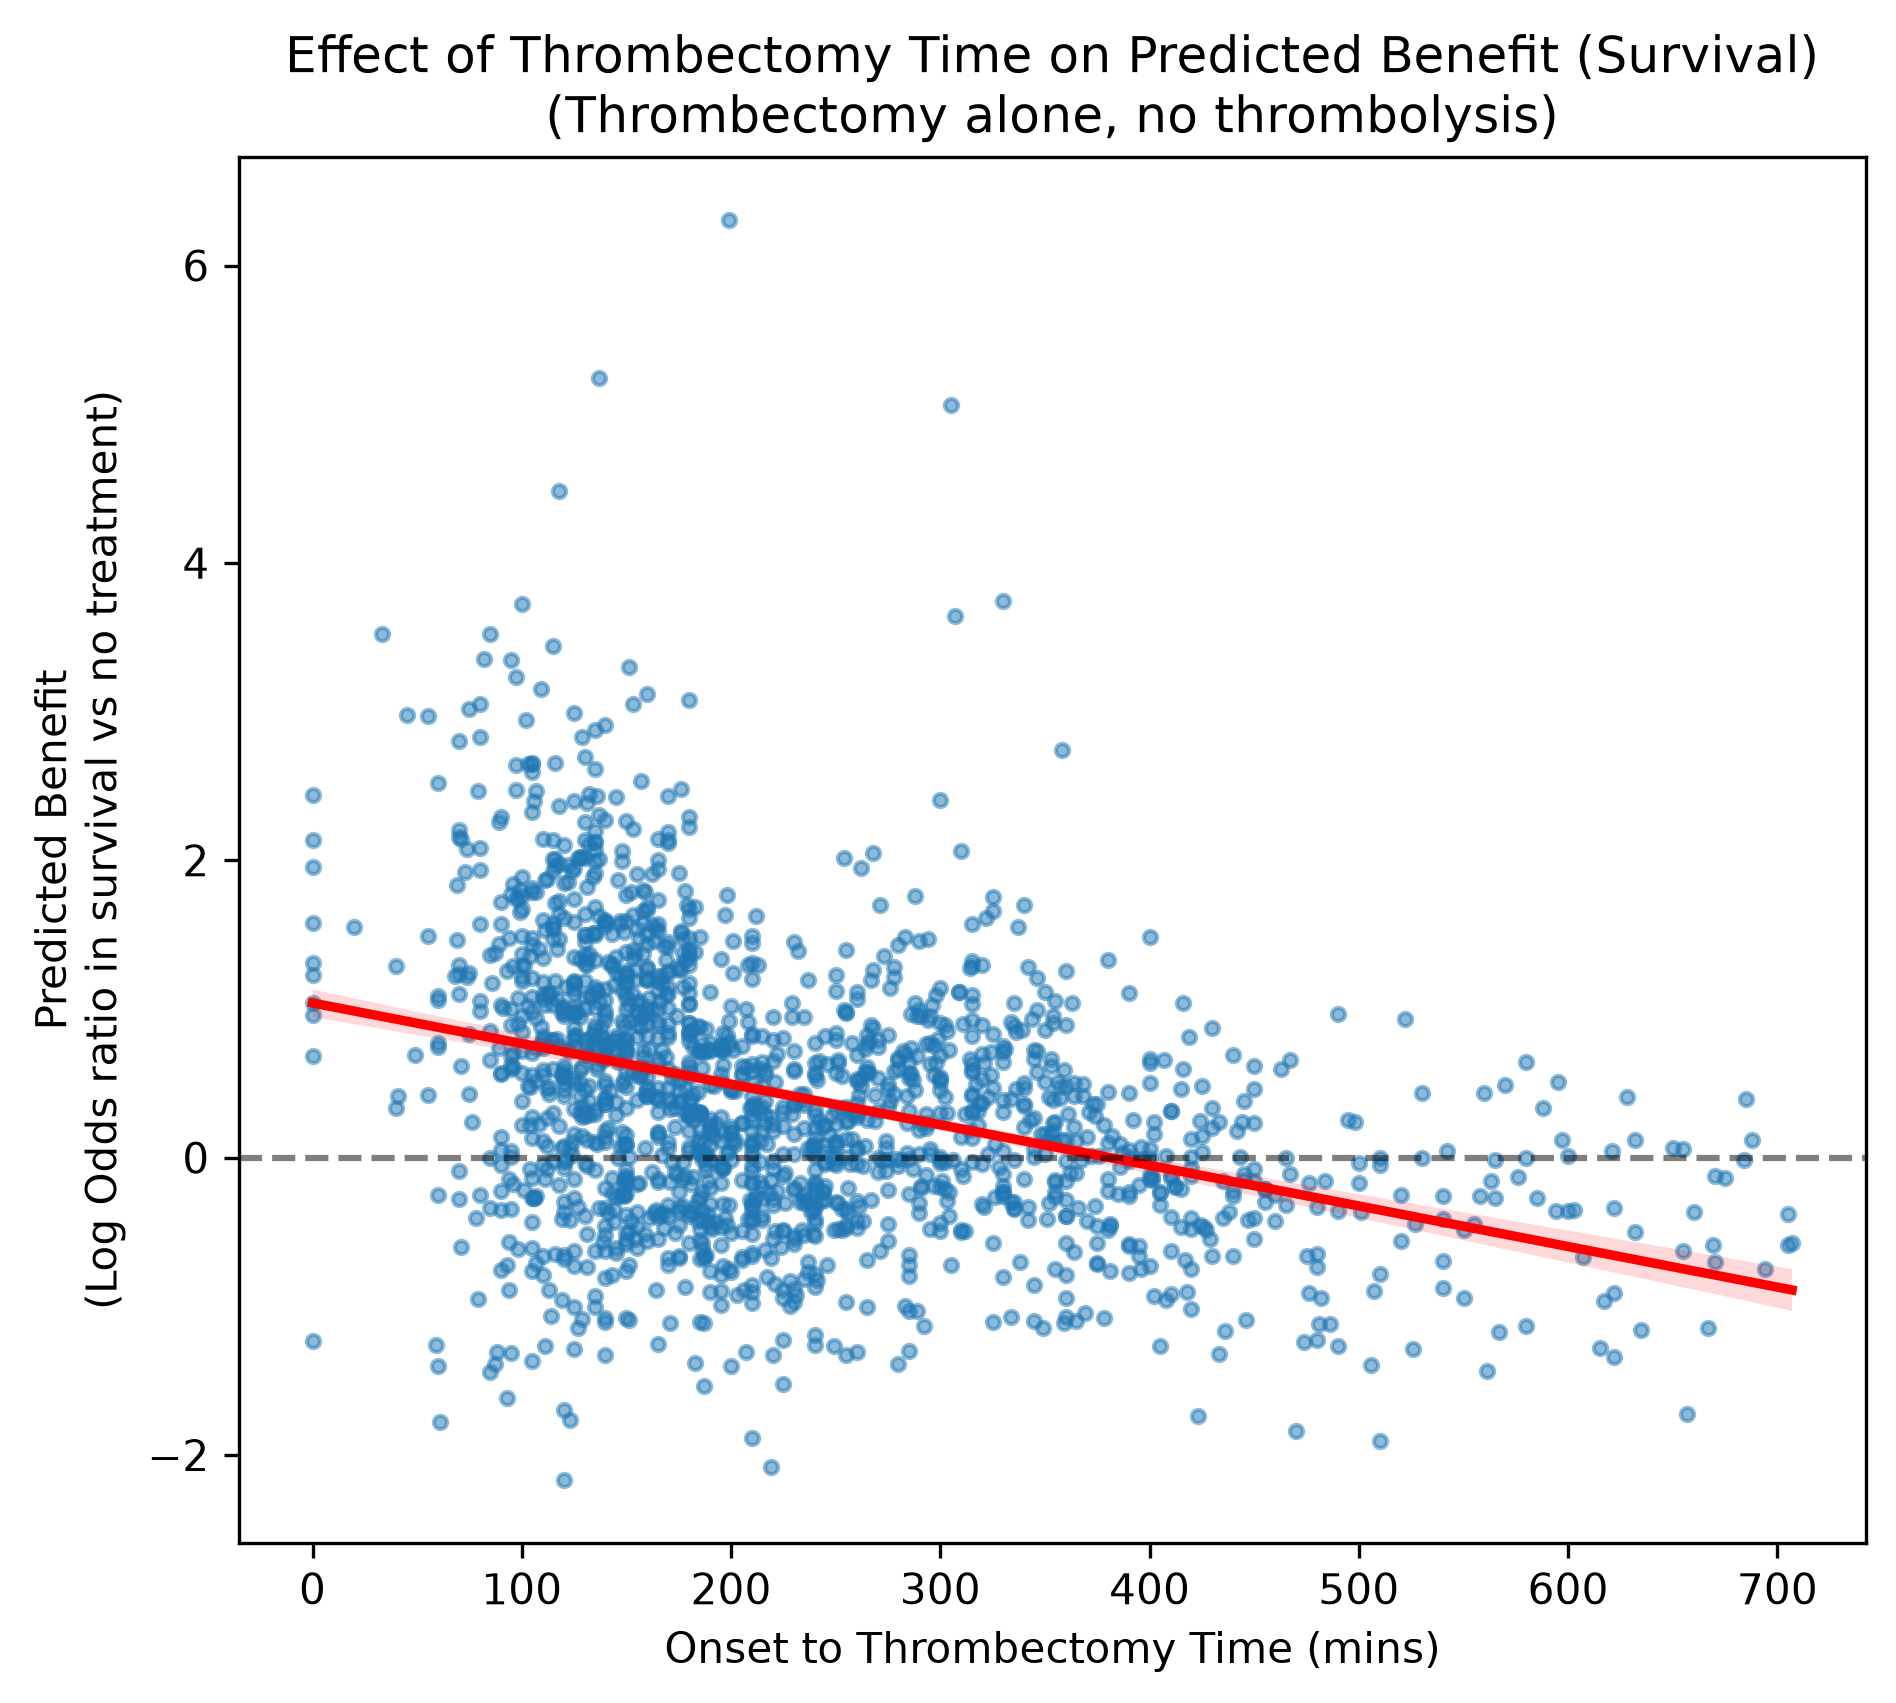
\includegraphics[width=\linewidth]{images/treatment_effects/thrombectomy_alone_time_effect_mrs_2.png}
        %\caption{}
    \end{subfigure}

    \vspace{0.2cm} % Optional vertical space between rows

    % Center left image
    \begin{subfigure}{0.38\textwidth}
        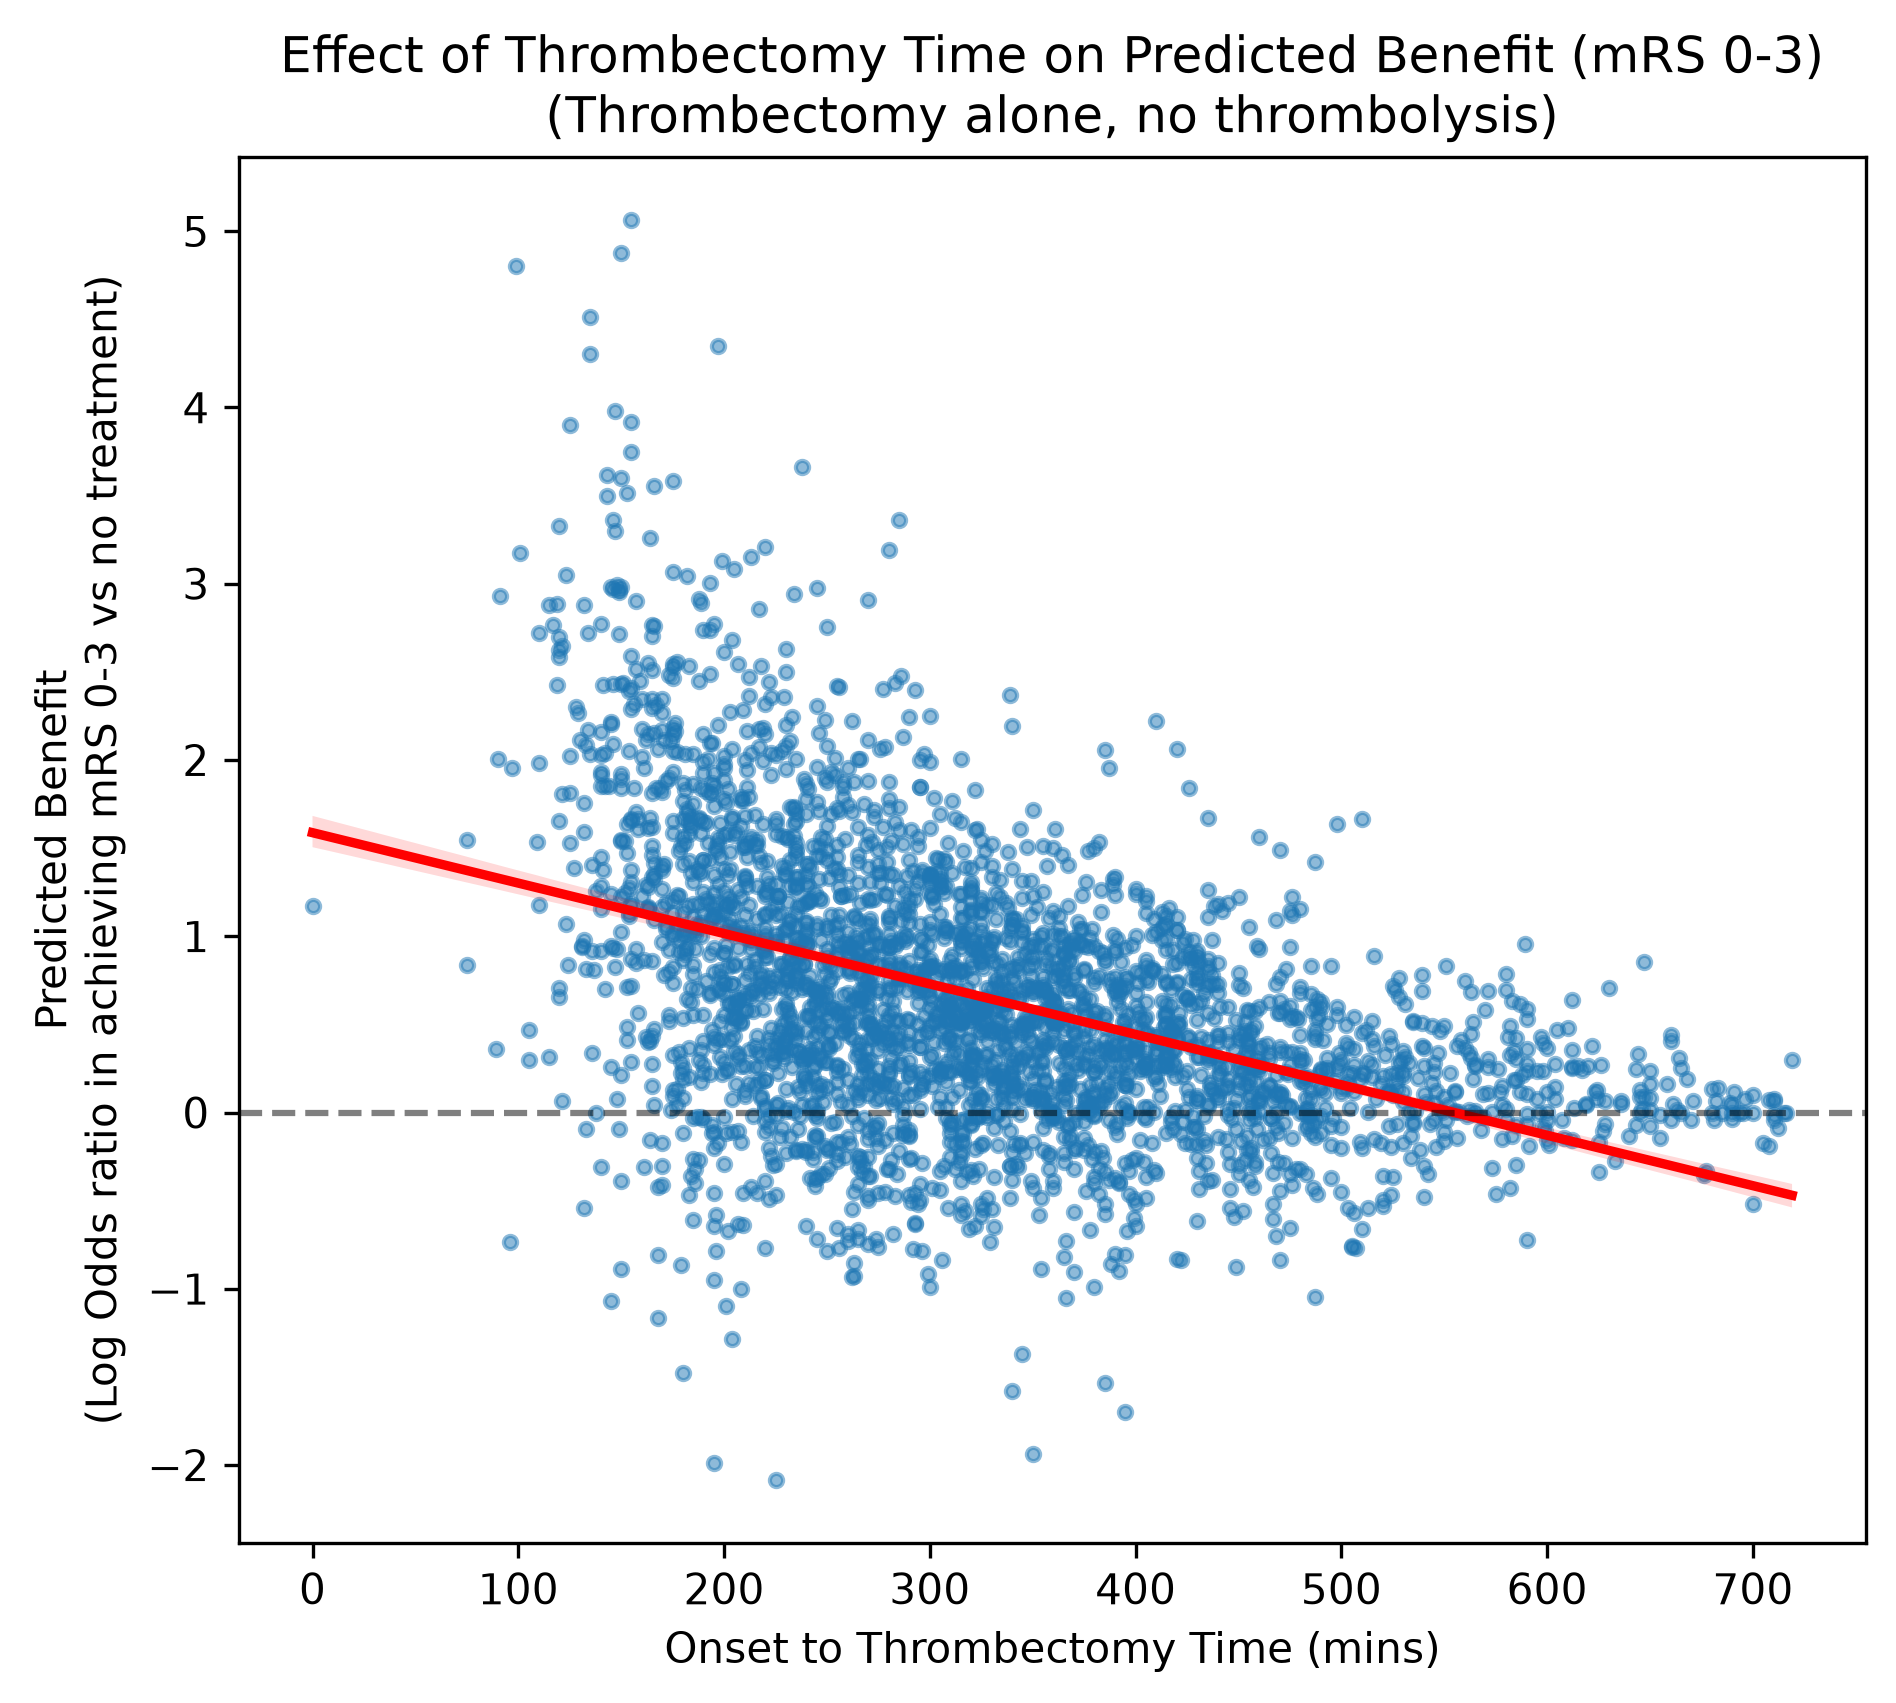
\includegraphics[width=\linewidth]{images/treatment_effects/thrombectomy_alone_time_effect_mrs_3.png}
        %\caption{}
    \end{subfigure}
    %\hfill{} % Adds flexible horizontal spacing
    % Centre right image 
    \begin{subfigure}{0.38\textwidth}
        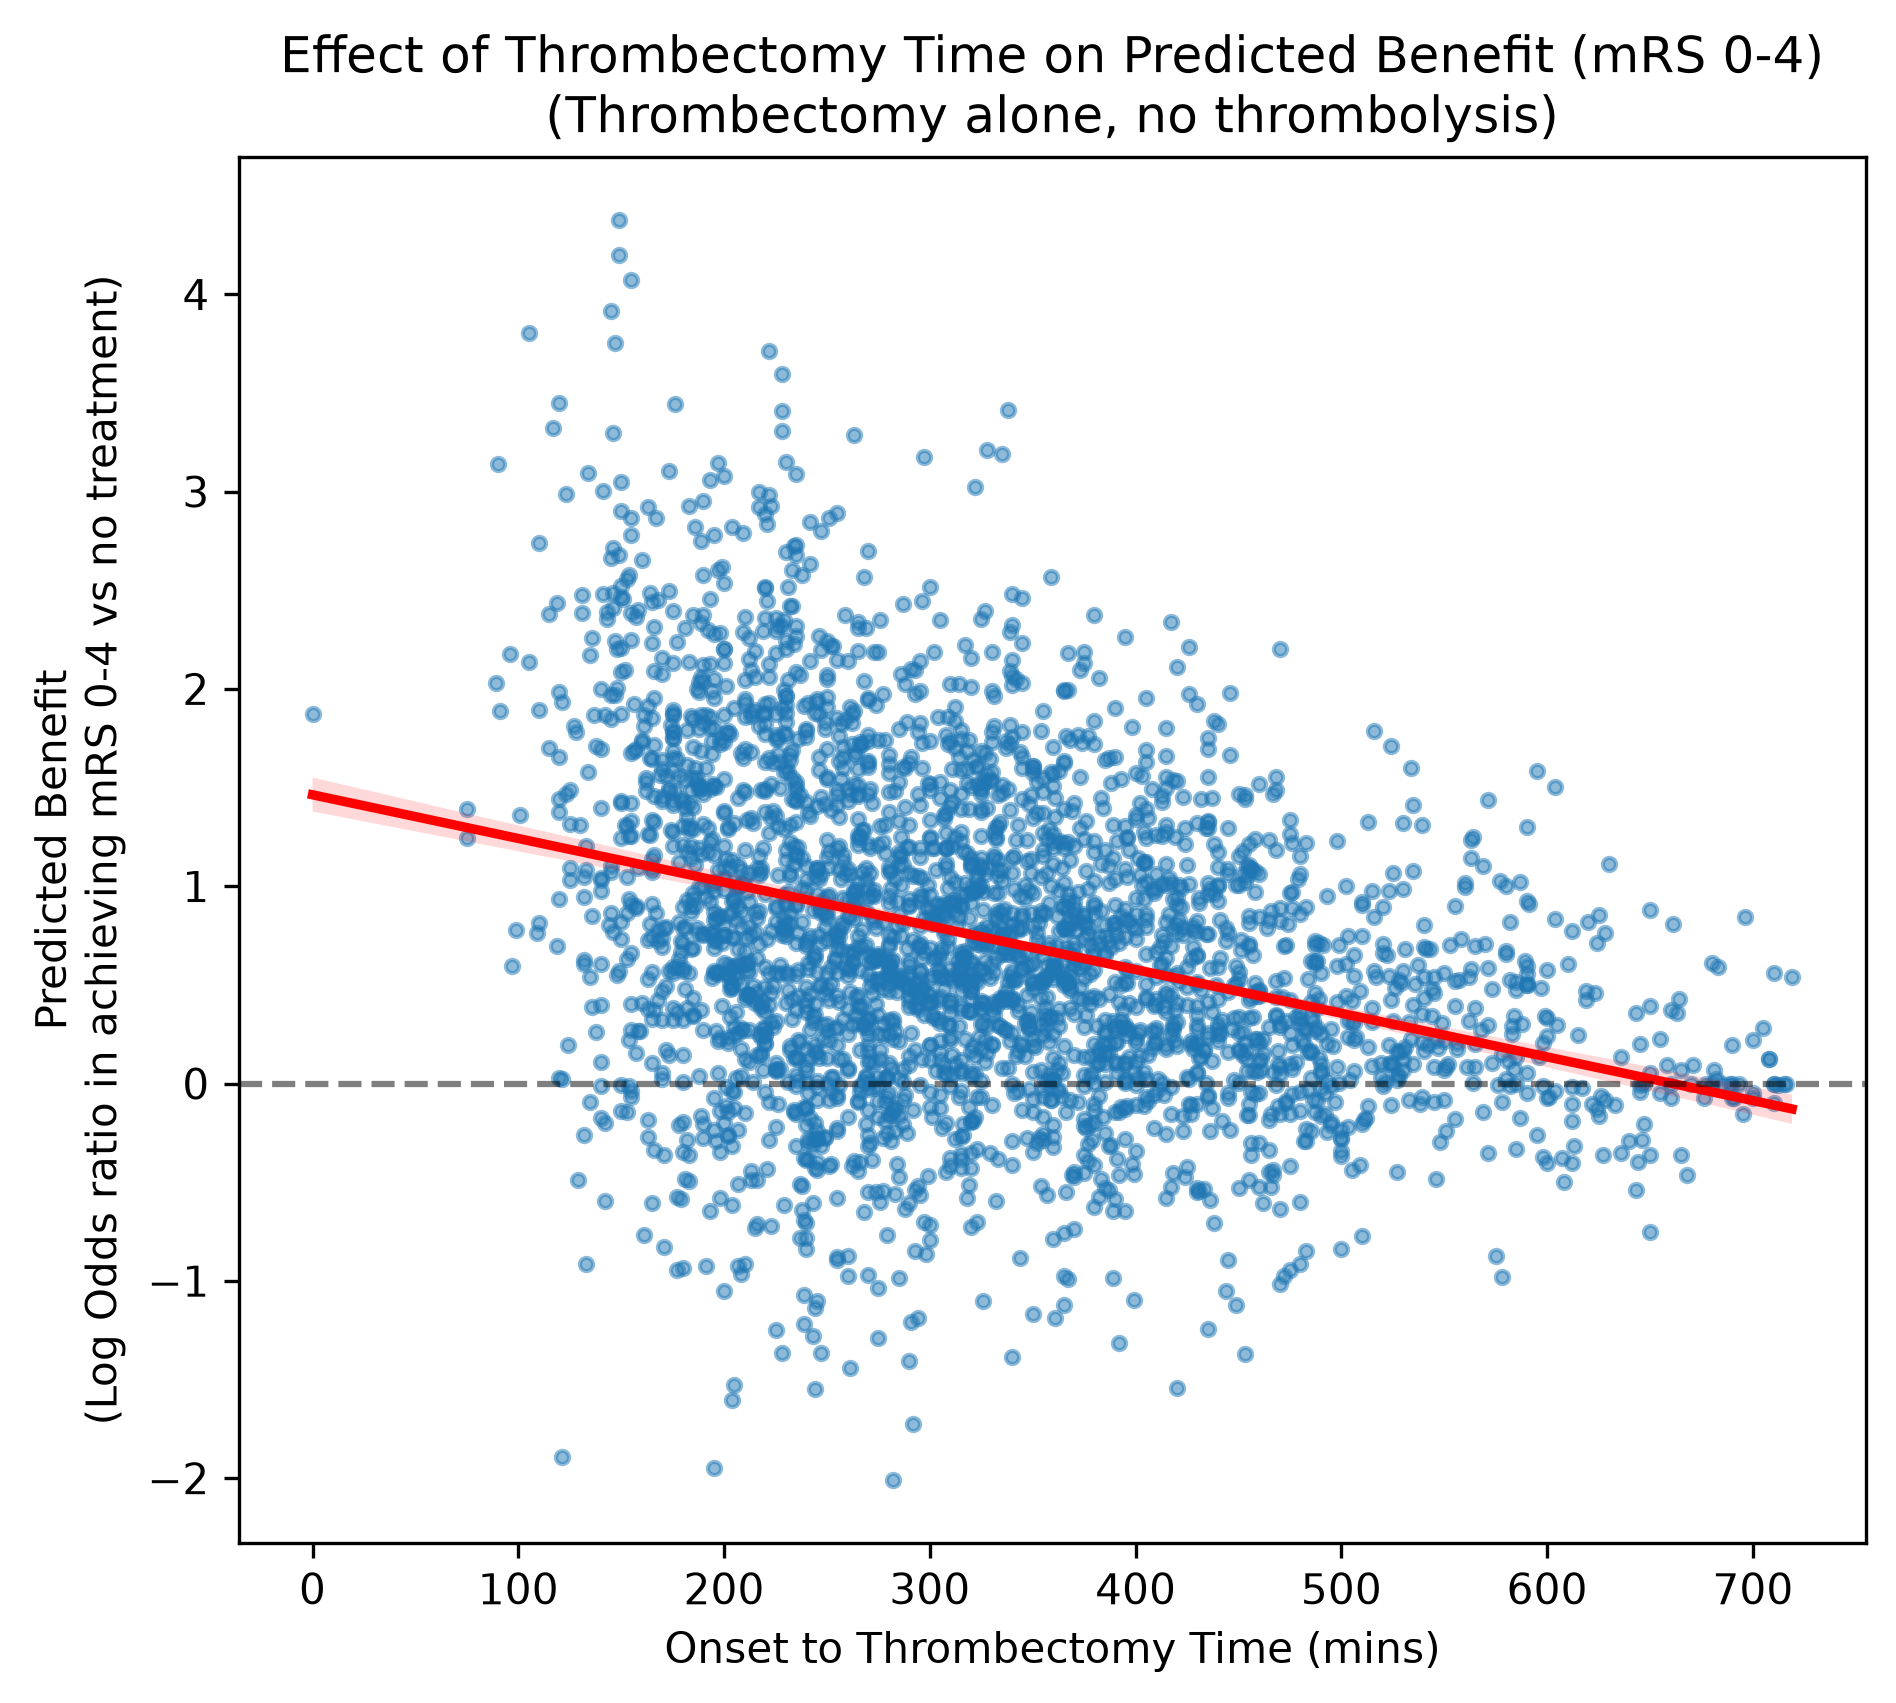
\includegraphics[width=\linewidth]{images/treatment_effects/thrombectomy_alone_time_effect_mrs_4.png}
        %\caption{}
    \end{subfigure}

    \vspace{0.2cm} % Optional vertical space between rows

    % Bottom image
    \begin{subfigure}{0.38\textwidth}
        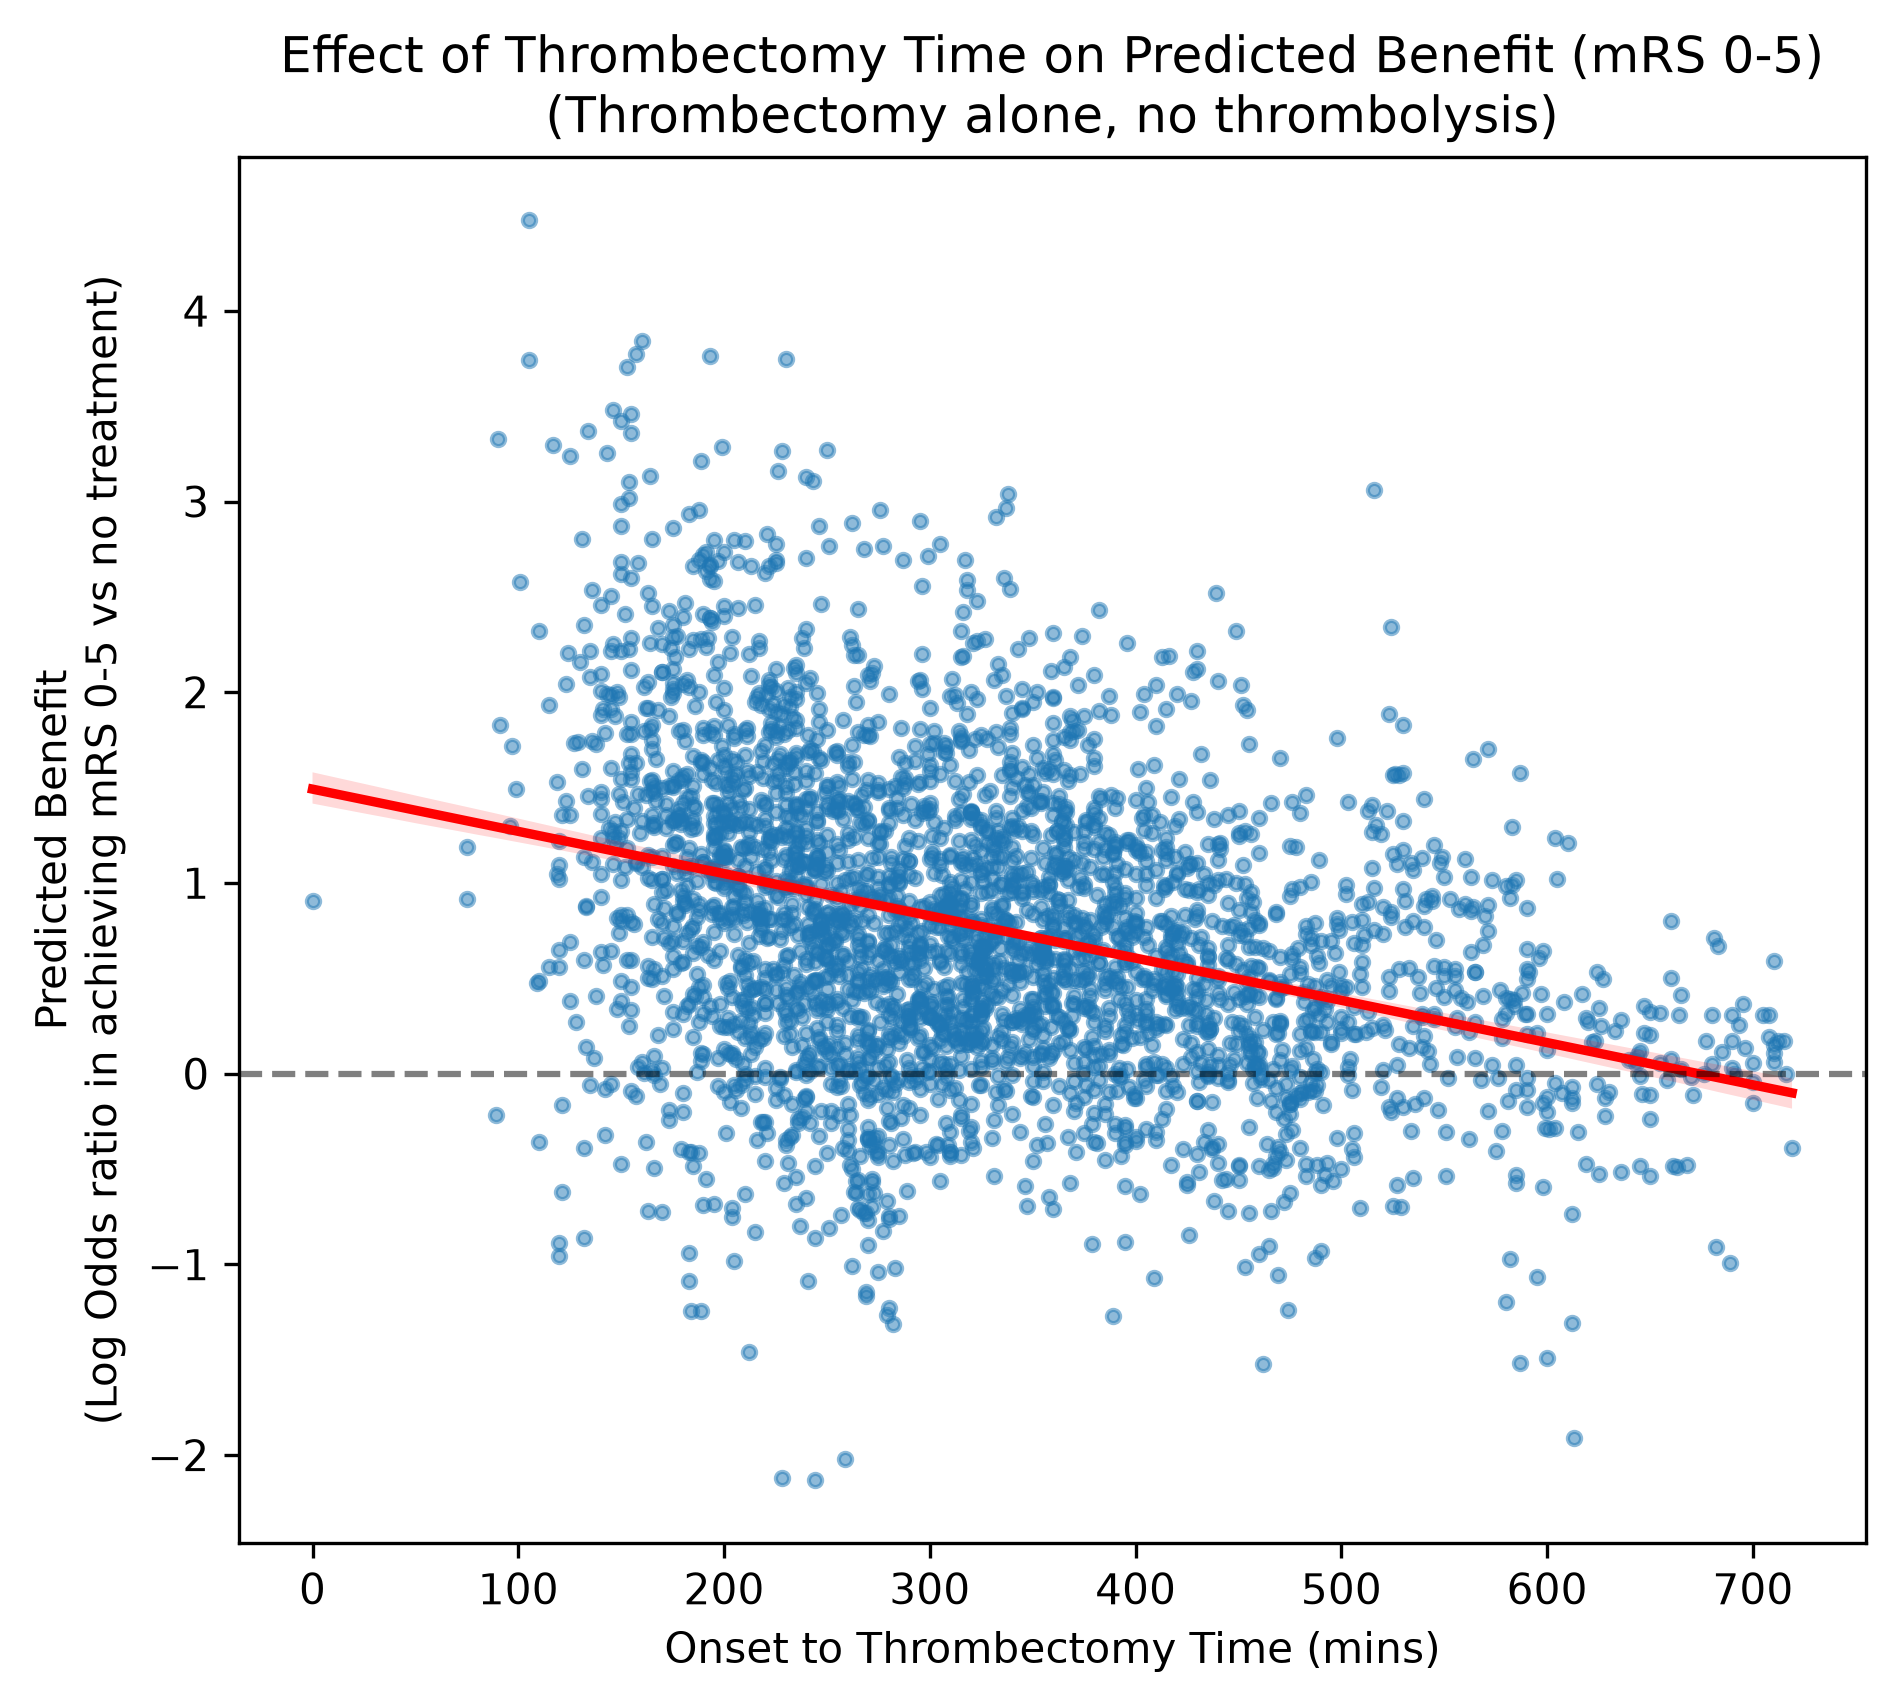
\includegraphics[width=\linewidth]{images/treatment_effects/thrombectomy_alone_time_effect_mrs_5}
        %\caption{}
    \end{subfigure}
    
    \caption{Association between onset-to-thrombectomy time and individualised predicted benefit of thrombectomy alone, estimated using the S-learner XGBoost model. Each panel shows the predicted improvement in the odds of a good outcome (discharge at or below the specified modified Rankin Scale (mRS) threshold, or no worse than the pre-stroke mRS). Analyses are restricted to patients receiving mechanical thrombectomy without intravenous thrombolysis; each point represents an individual patient. The vertical axis shows the model-estimated treatment benefit on the log-odds scale, relative to the counterfactual prediction under no treatment. The red line denotes the fitted linear trend, illustrating the decline in predicted benefit with increasing onset-to-thrombectomy time. The dashed horizontal line indicates no predicted treatment benefit (log-odds ratio = 0); values above and below this line indicate predicted benefit and harm, respectively.}
    \label{fig:s_learner_time_thrombectomy}
\end{figure}





% S-learner SHAP benefit

\subsubsection{SHAP for S-learner predicted benefit}

To understand which patients benefited most, a secondary XGBoost model was fitted to predict each treated patient's estimated benefit (from the S-learner) from their characteristics and treatment, and SHAP values were calculated for this model. Figures \ref{fig:s_learner_benefit_shap_mrs_1} to \ref{fig:s_learner_benefit_shap_mrs_5} show these SHAP values for each mRS threshold. For each feature, the box plots show how the feature's values were associated with higher (positive SHAP value) or lower (negative SHAP value) predicted benefit than average. As with the other SHAP analyses in this supplement, these associations describe how the model makes its predictions and should not, on their own, be interpreted as causal.


\begin{figure}
    \centering
    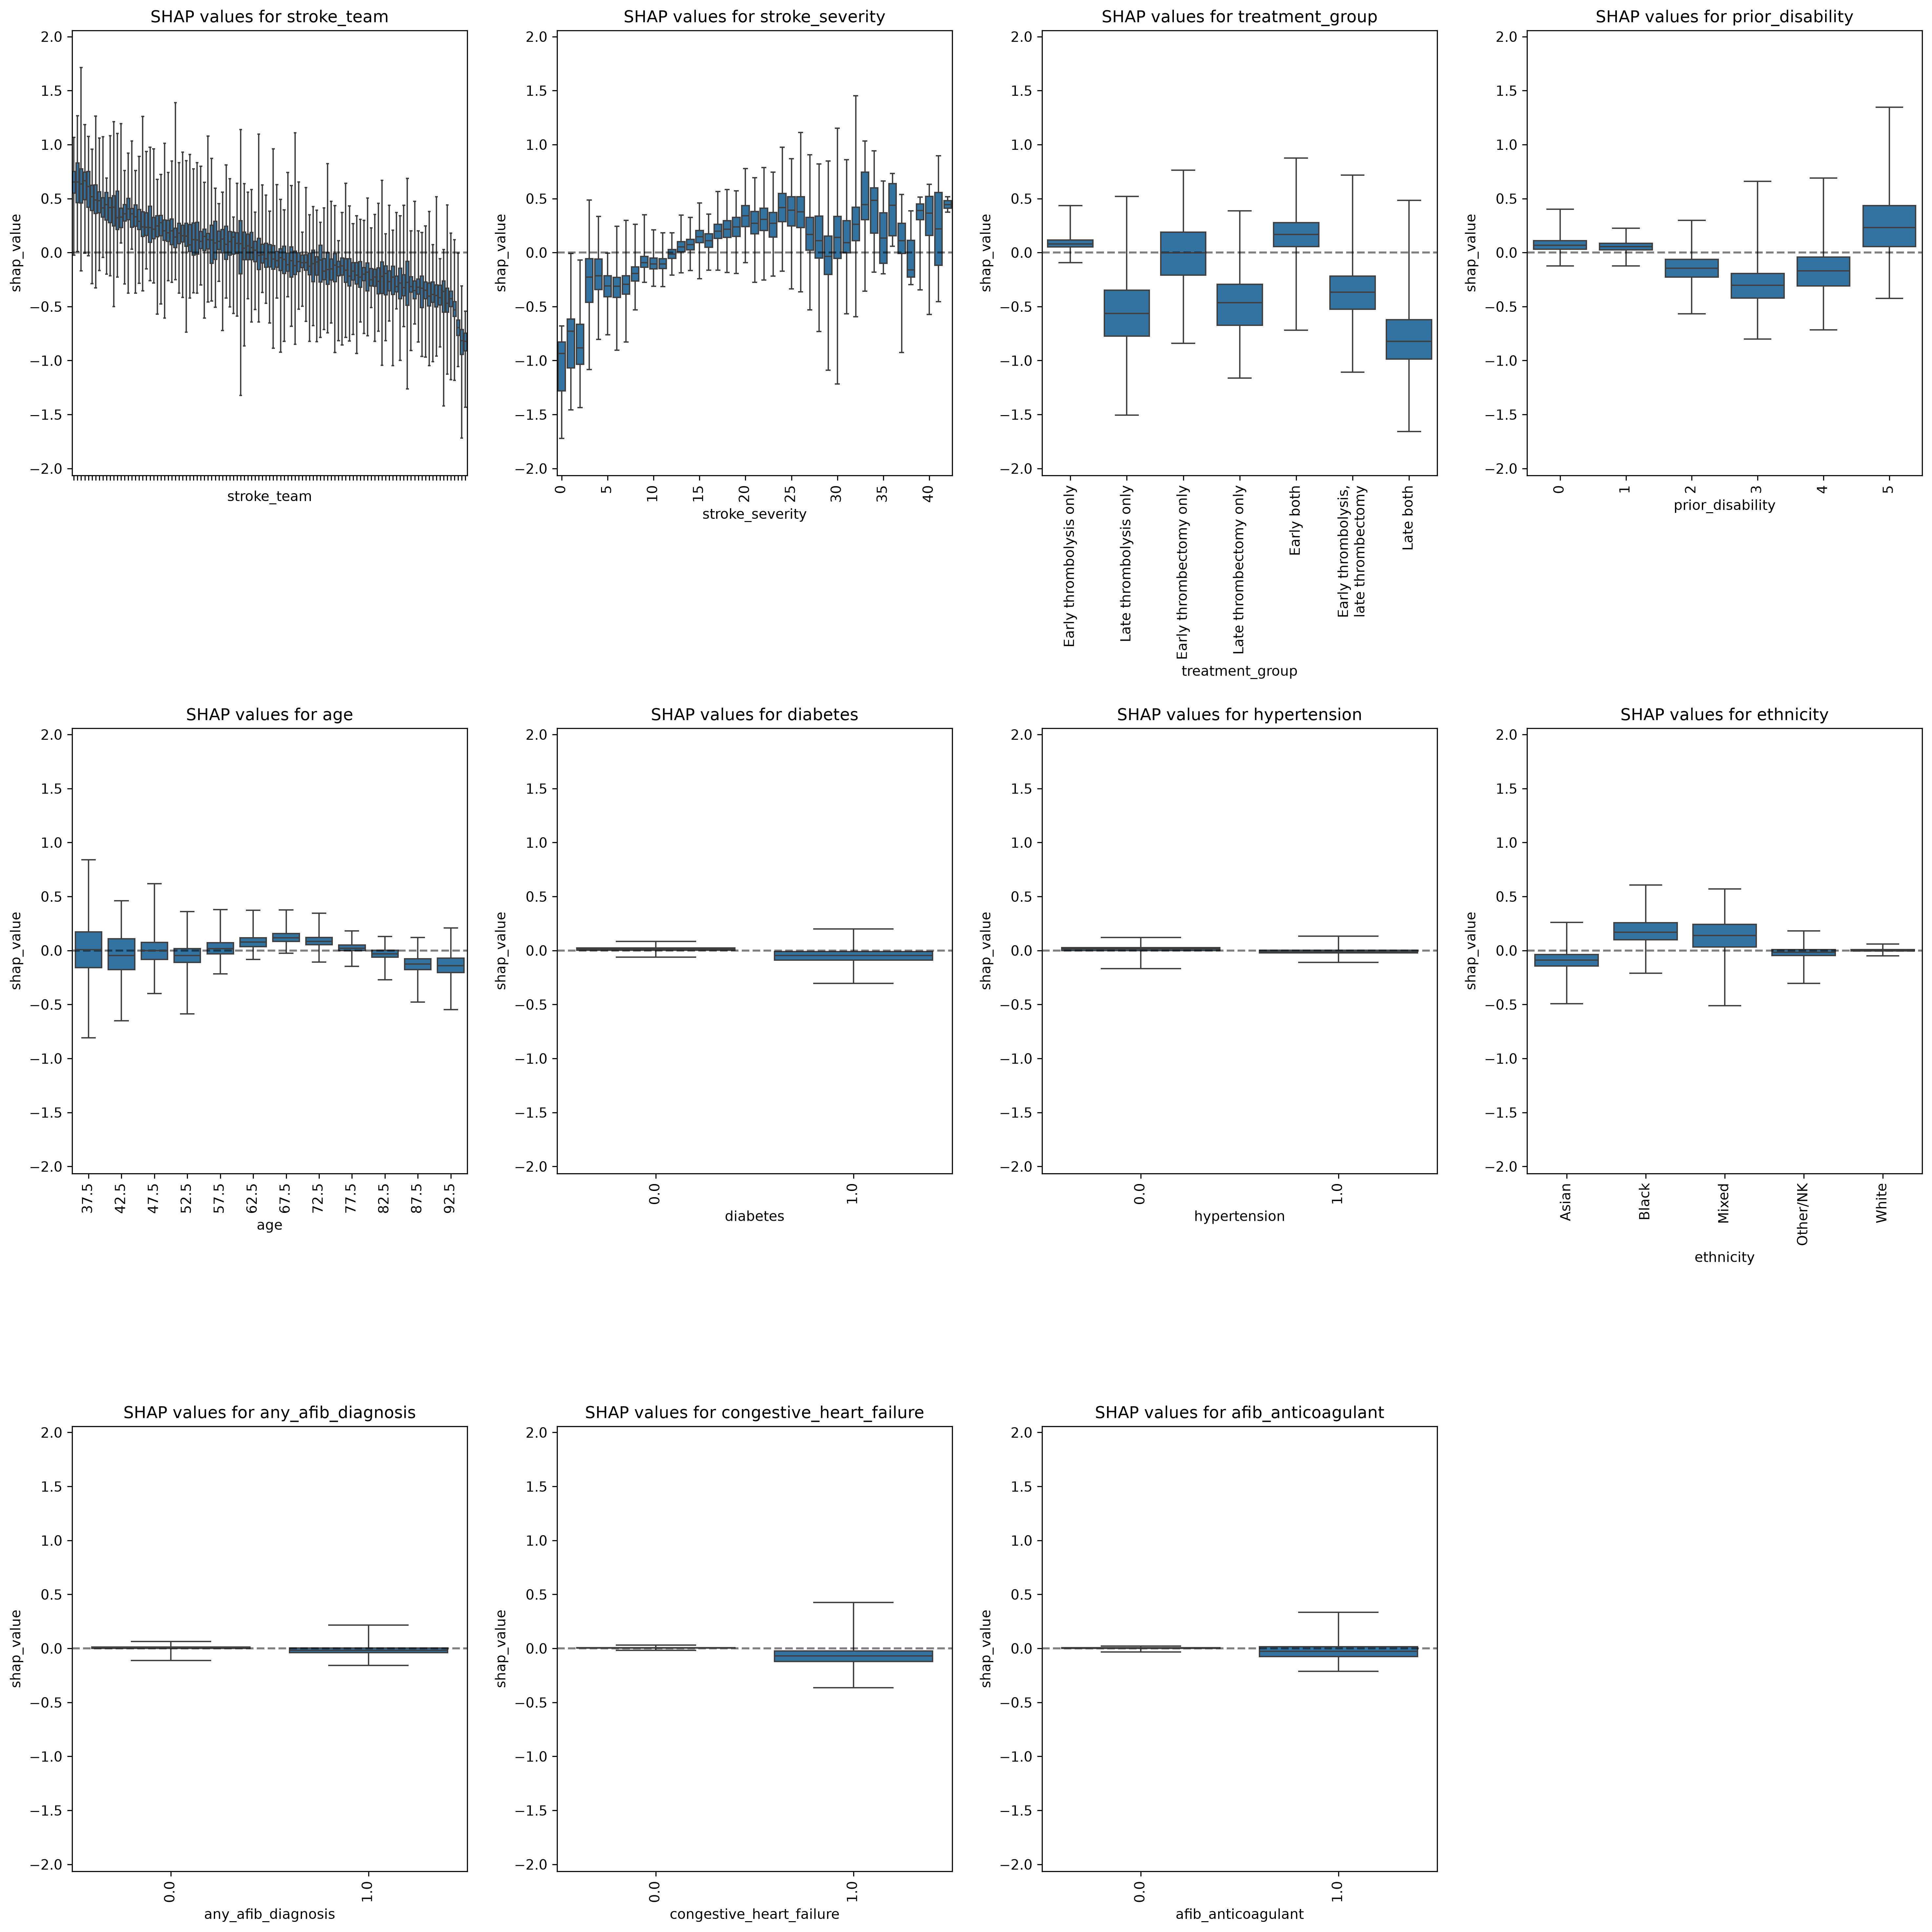
\includegraphics[width=1\linewidth]
{images/treatment_effects/s_learner_shap_box_plots_1.png}
    \caption{Effect of patient feature values on the predicted benefit of treatment. Subplots (top to bottom, left to right) are ordered by their average effect on benefit of treatment. Each subplot shows the feature value, and a boxplot of SHAP values for that feature value. The SHAP value is the contribution to the log-odds ratio treatment effect (treated vs untreated) for achieving a good outcome at the mRS 0–1 threshold.}
    \label{fig:s_learner_benefit_shap_mrs_1}
\end{figure}

\begin{figure}
    \centering
    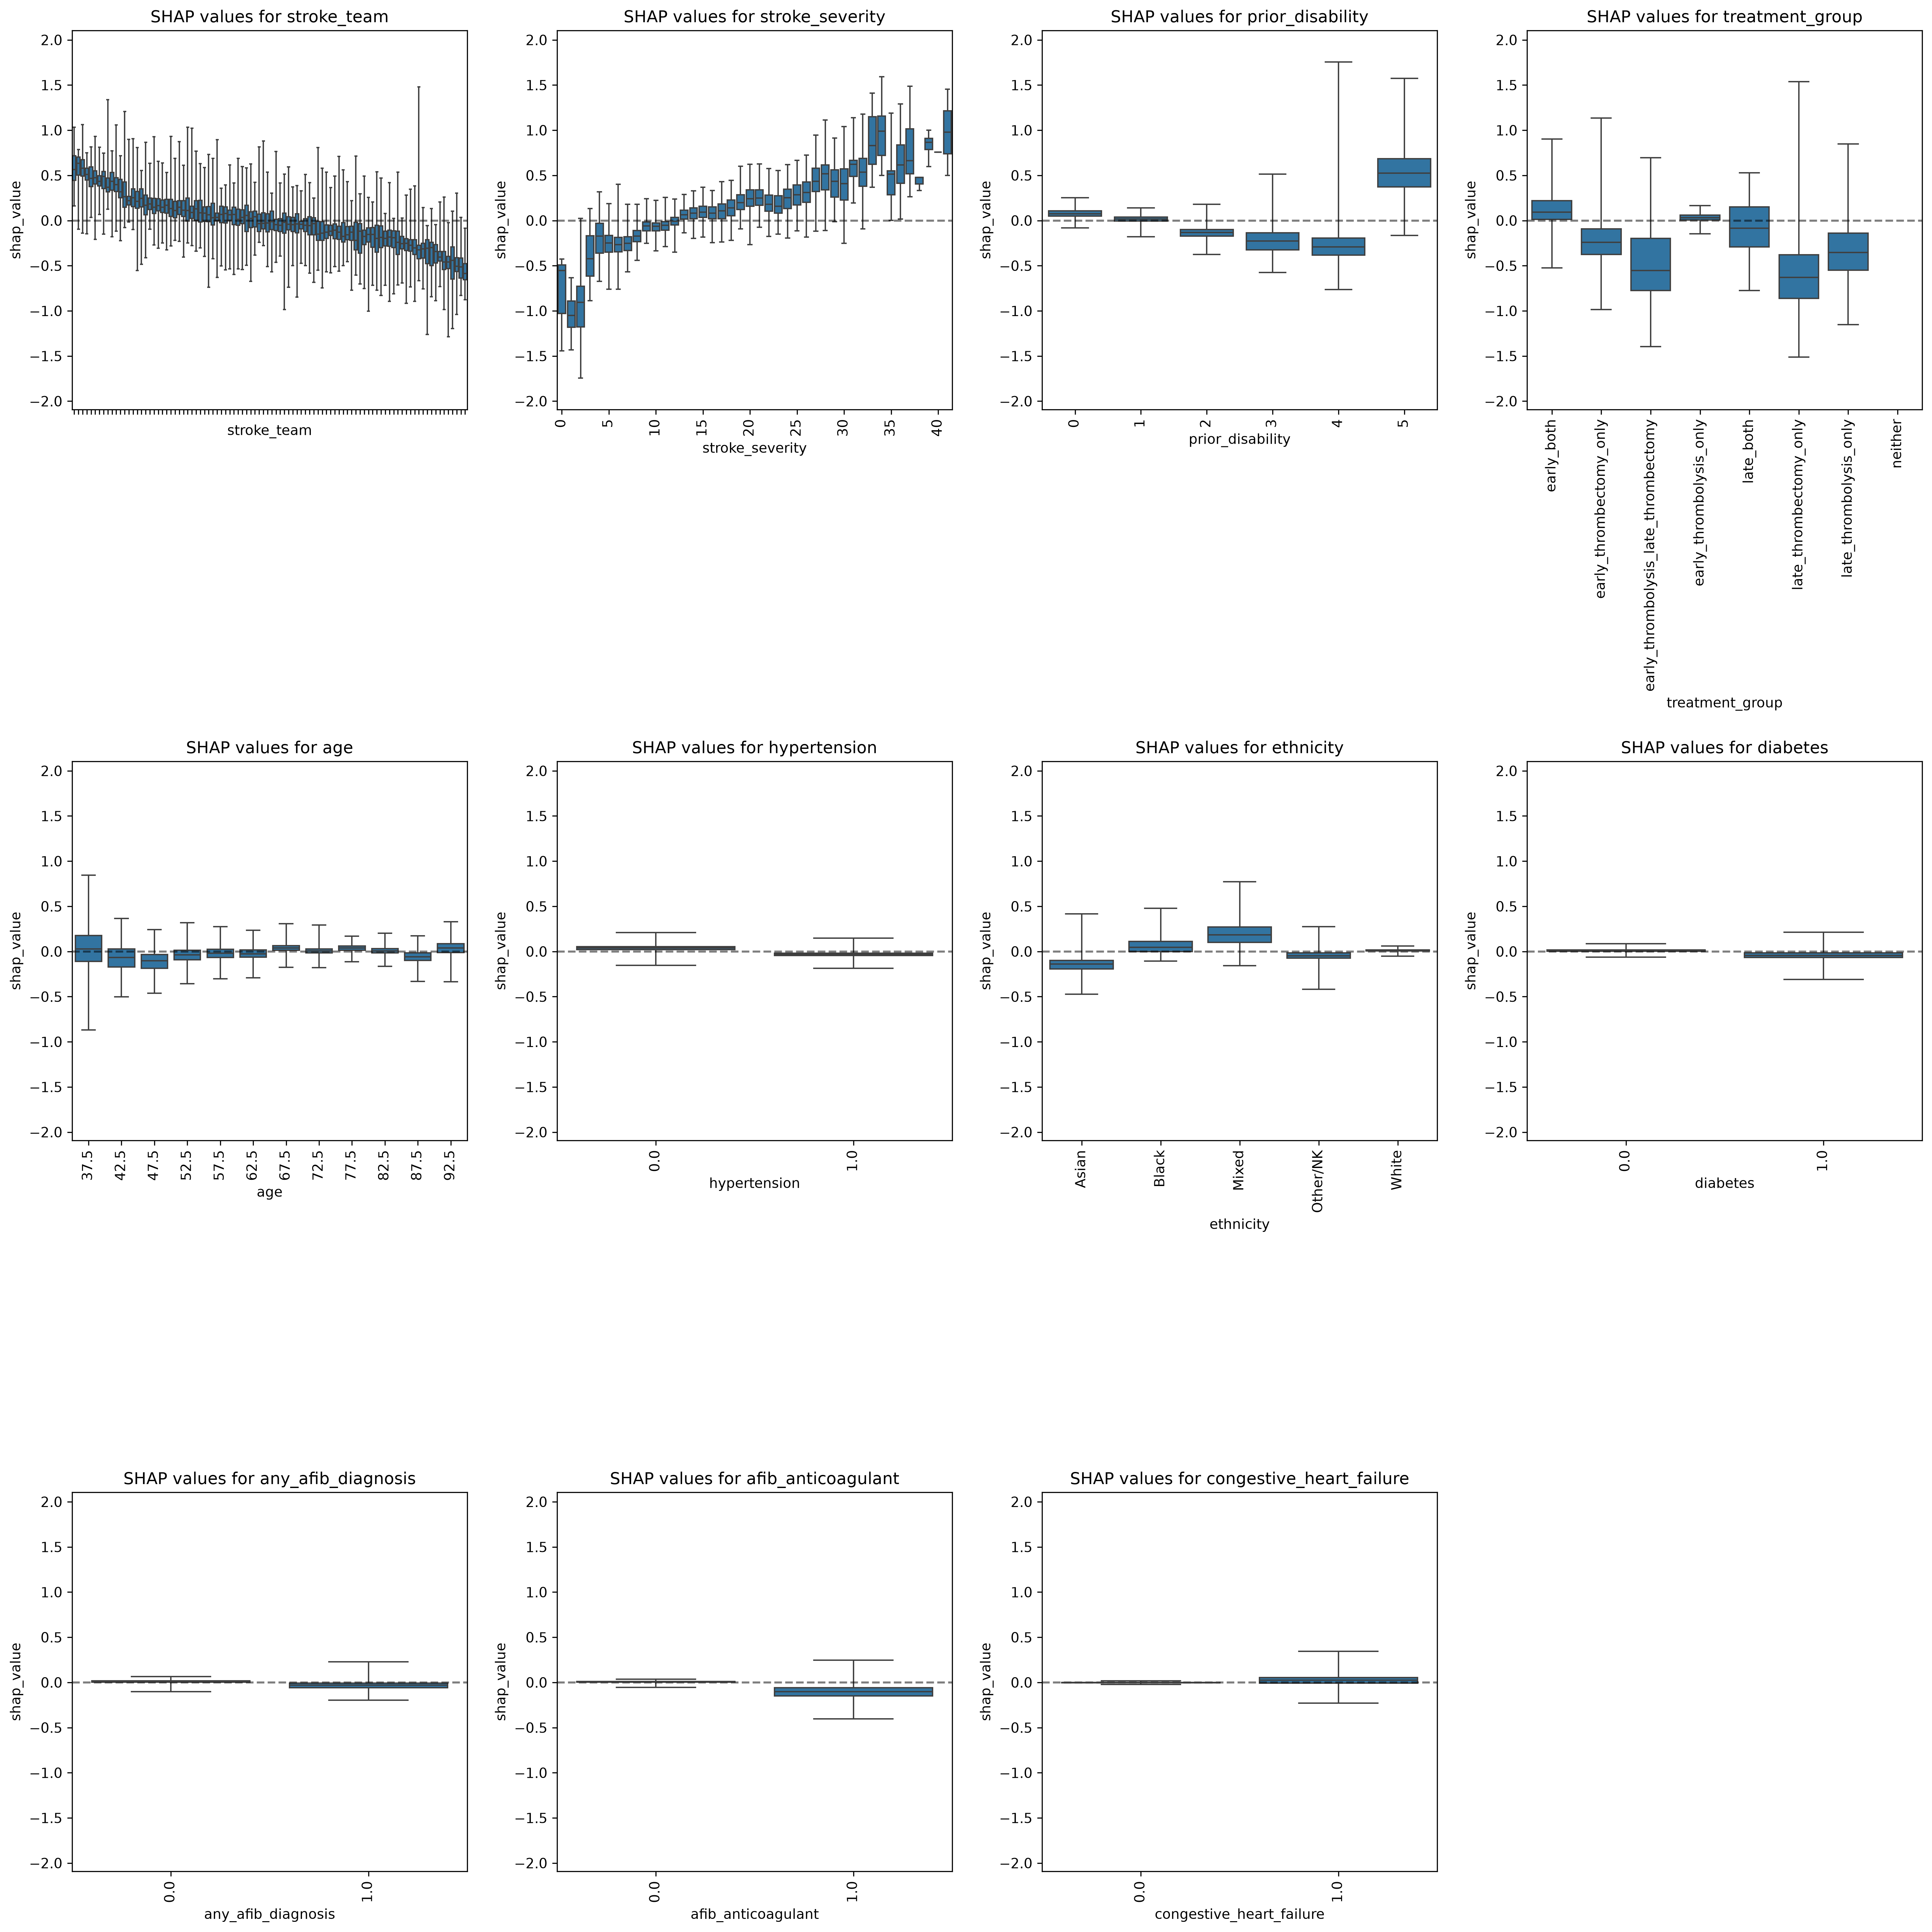
\includegraphics[width=1\linewidth]
{images/treatment_effects/s_learner_shap_box_plots_2.png}
    \caption{Effect of patient feature values on the predicted benefit of treatment. Subplots (top to bottom, left to right) are ordered by their average effect on benefit of treatment. Each subplot shows the feature value, and a boxplot of SHAP values for that feature value. The SHAP value is the contribution to the log-odds ratio treatment effect (treated vs untreated) for achieving a good outcome at the mRS 0–2 threshold.}
    \label{fig:s_learner_benefit_shap_mrs_2}
\end{figure}

\begin{figure}
    \centering
    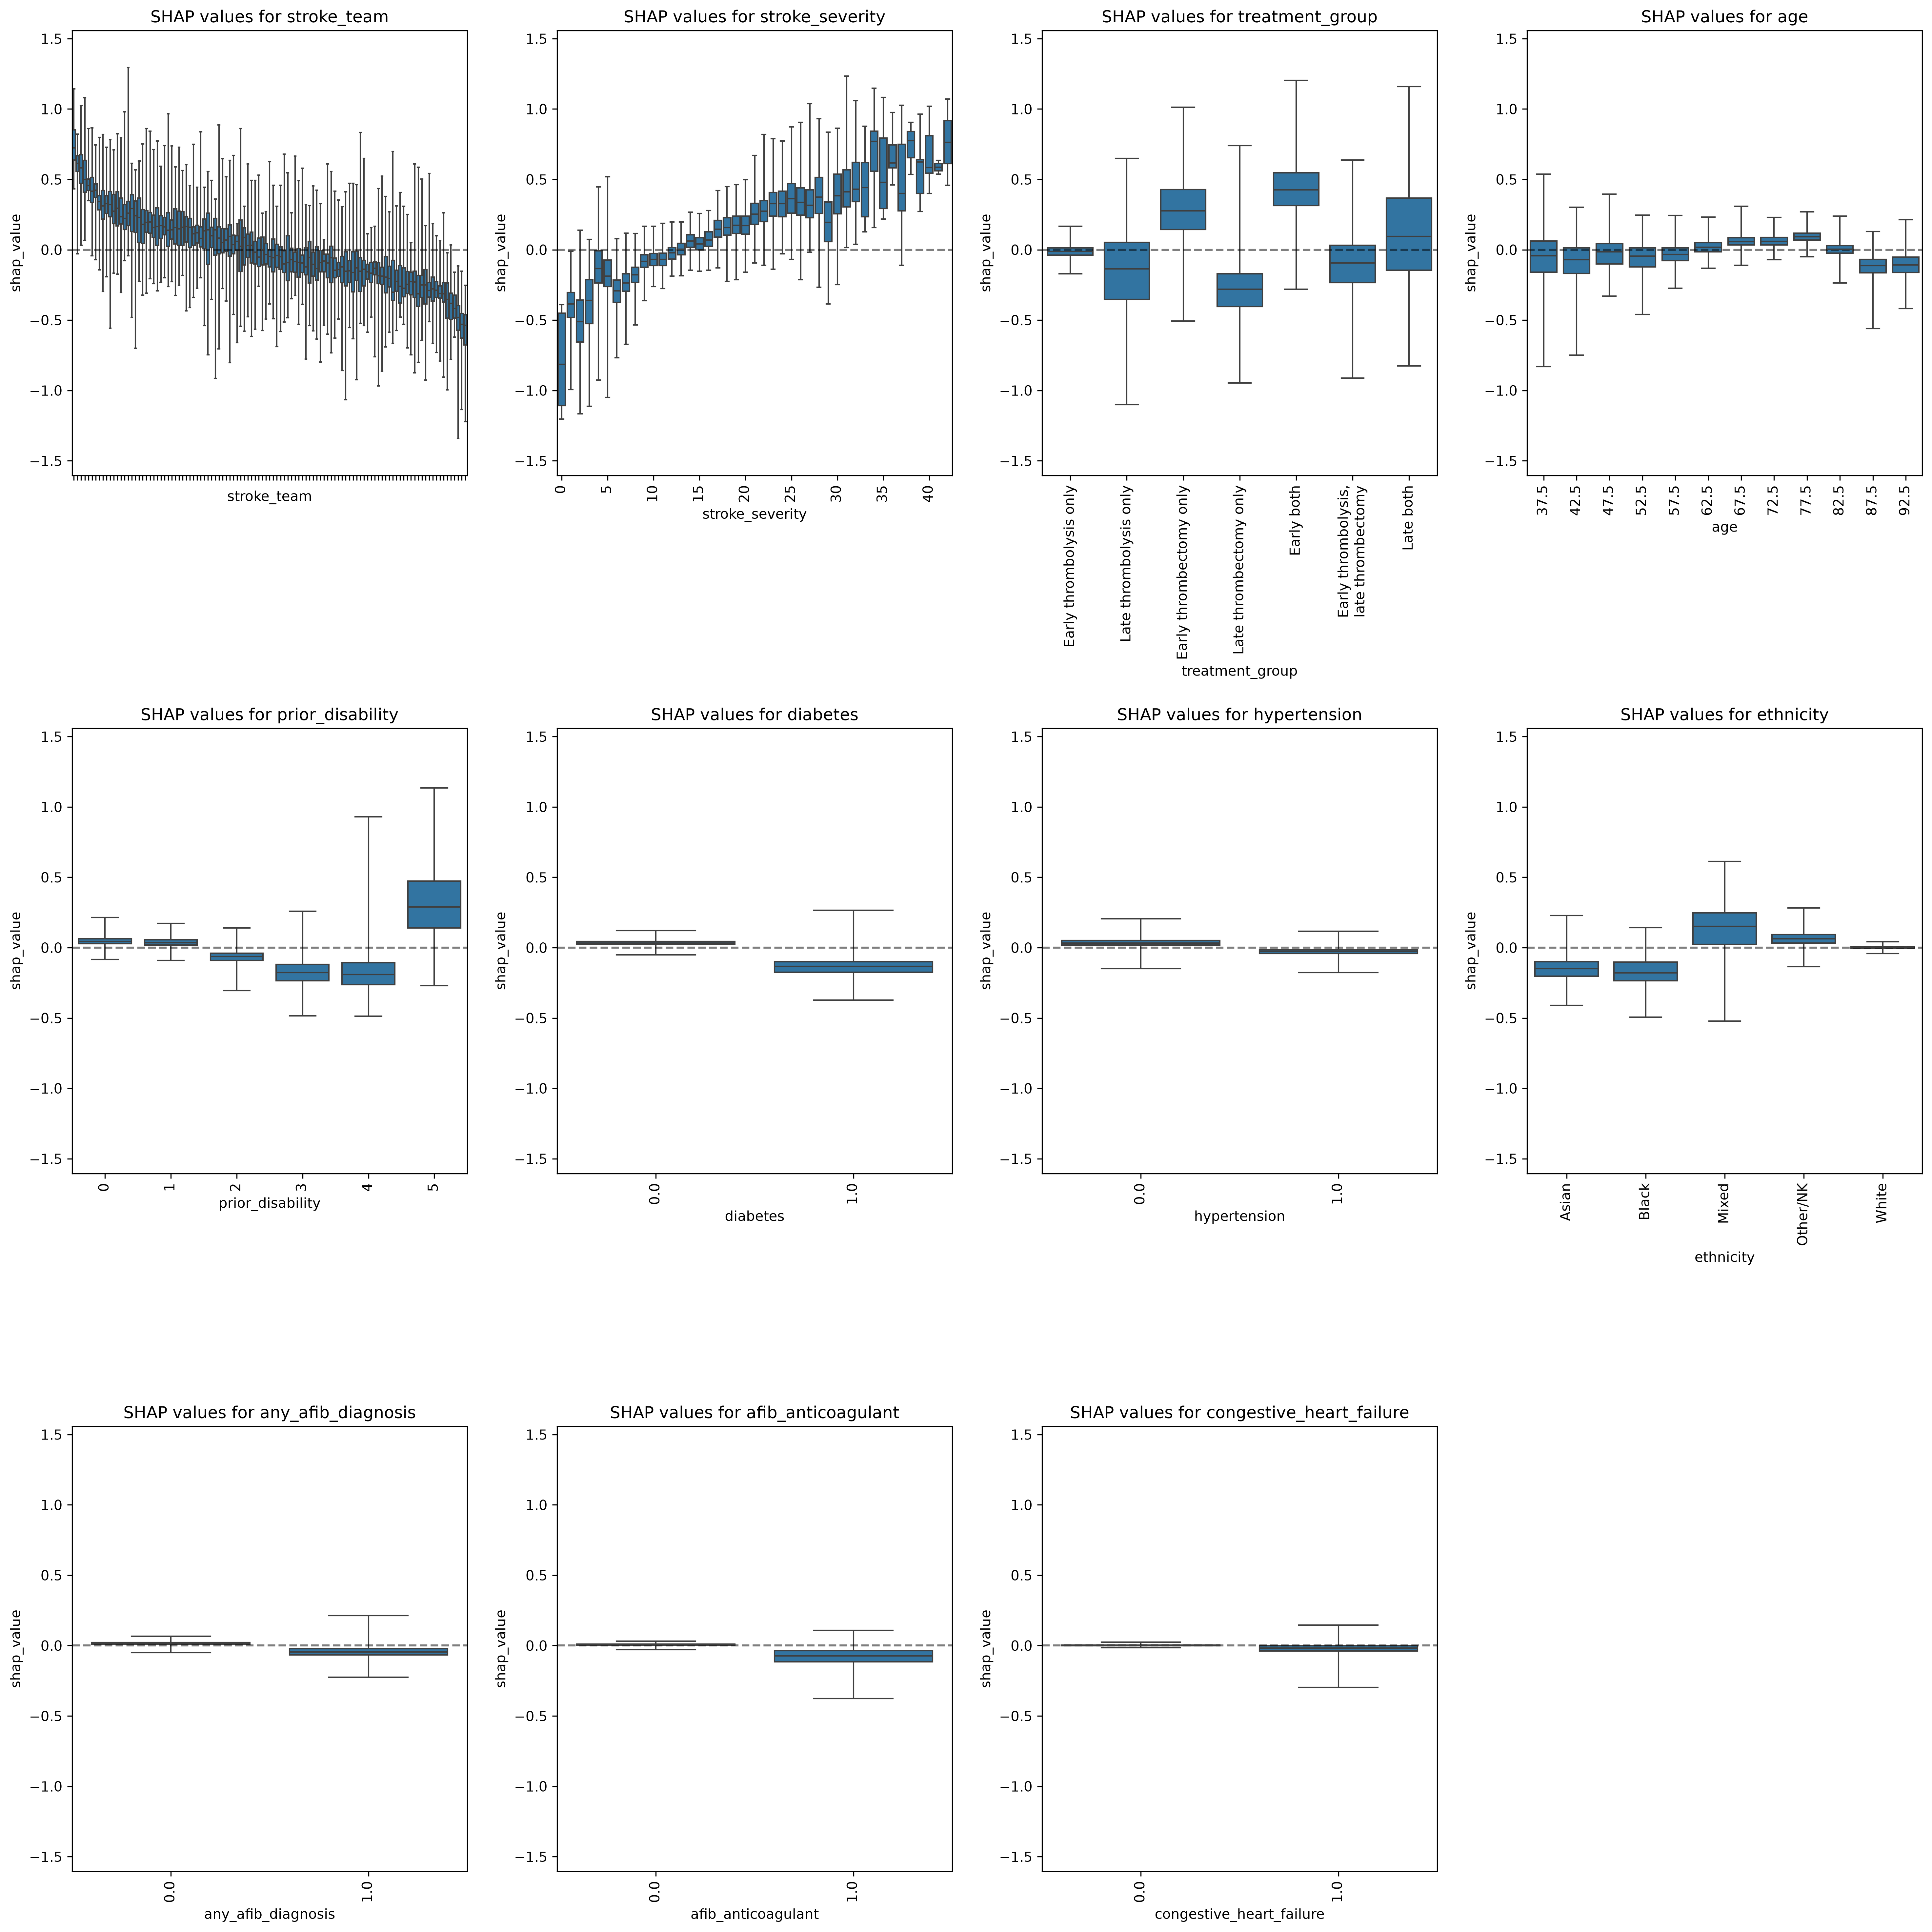
\includegraphics[width=1\linewidth]
{images/treatment_effects/s_learner_shap_box_plots_3.png}
    \caption{Effect of patient feature values on the predicted benefit of treatment. Subplots (top to bottom, left to right) are ordered by their average effect on benefit of treatment. Each subplot shows the feature value, and a boxplot of SHAP values for that feature value. The SHAP value is the contribution to the log-odds ratio treatment effect (treated vs untreated) for achieving a good outcome at the mRS 0–3 threshold.}
    \label{fig:s_learner_benefit_shap_mrs_3}
\end{figure}

\begin{figure}
    \centering
    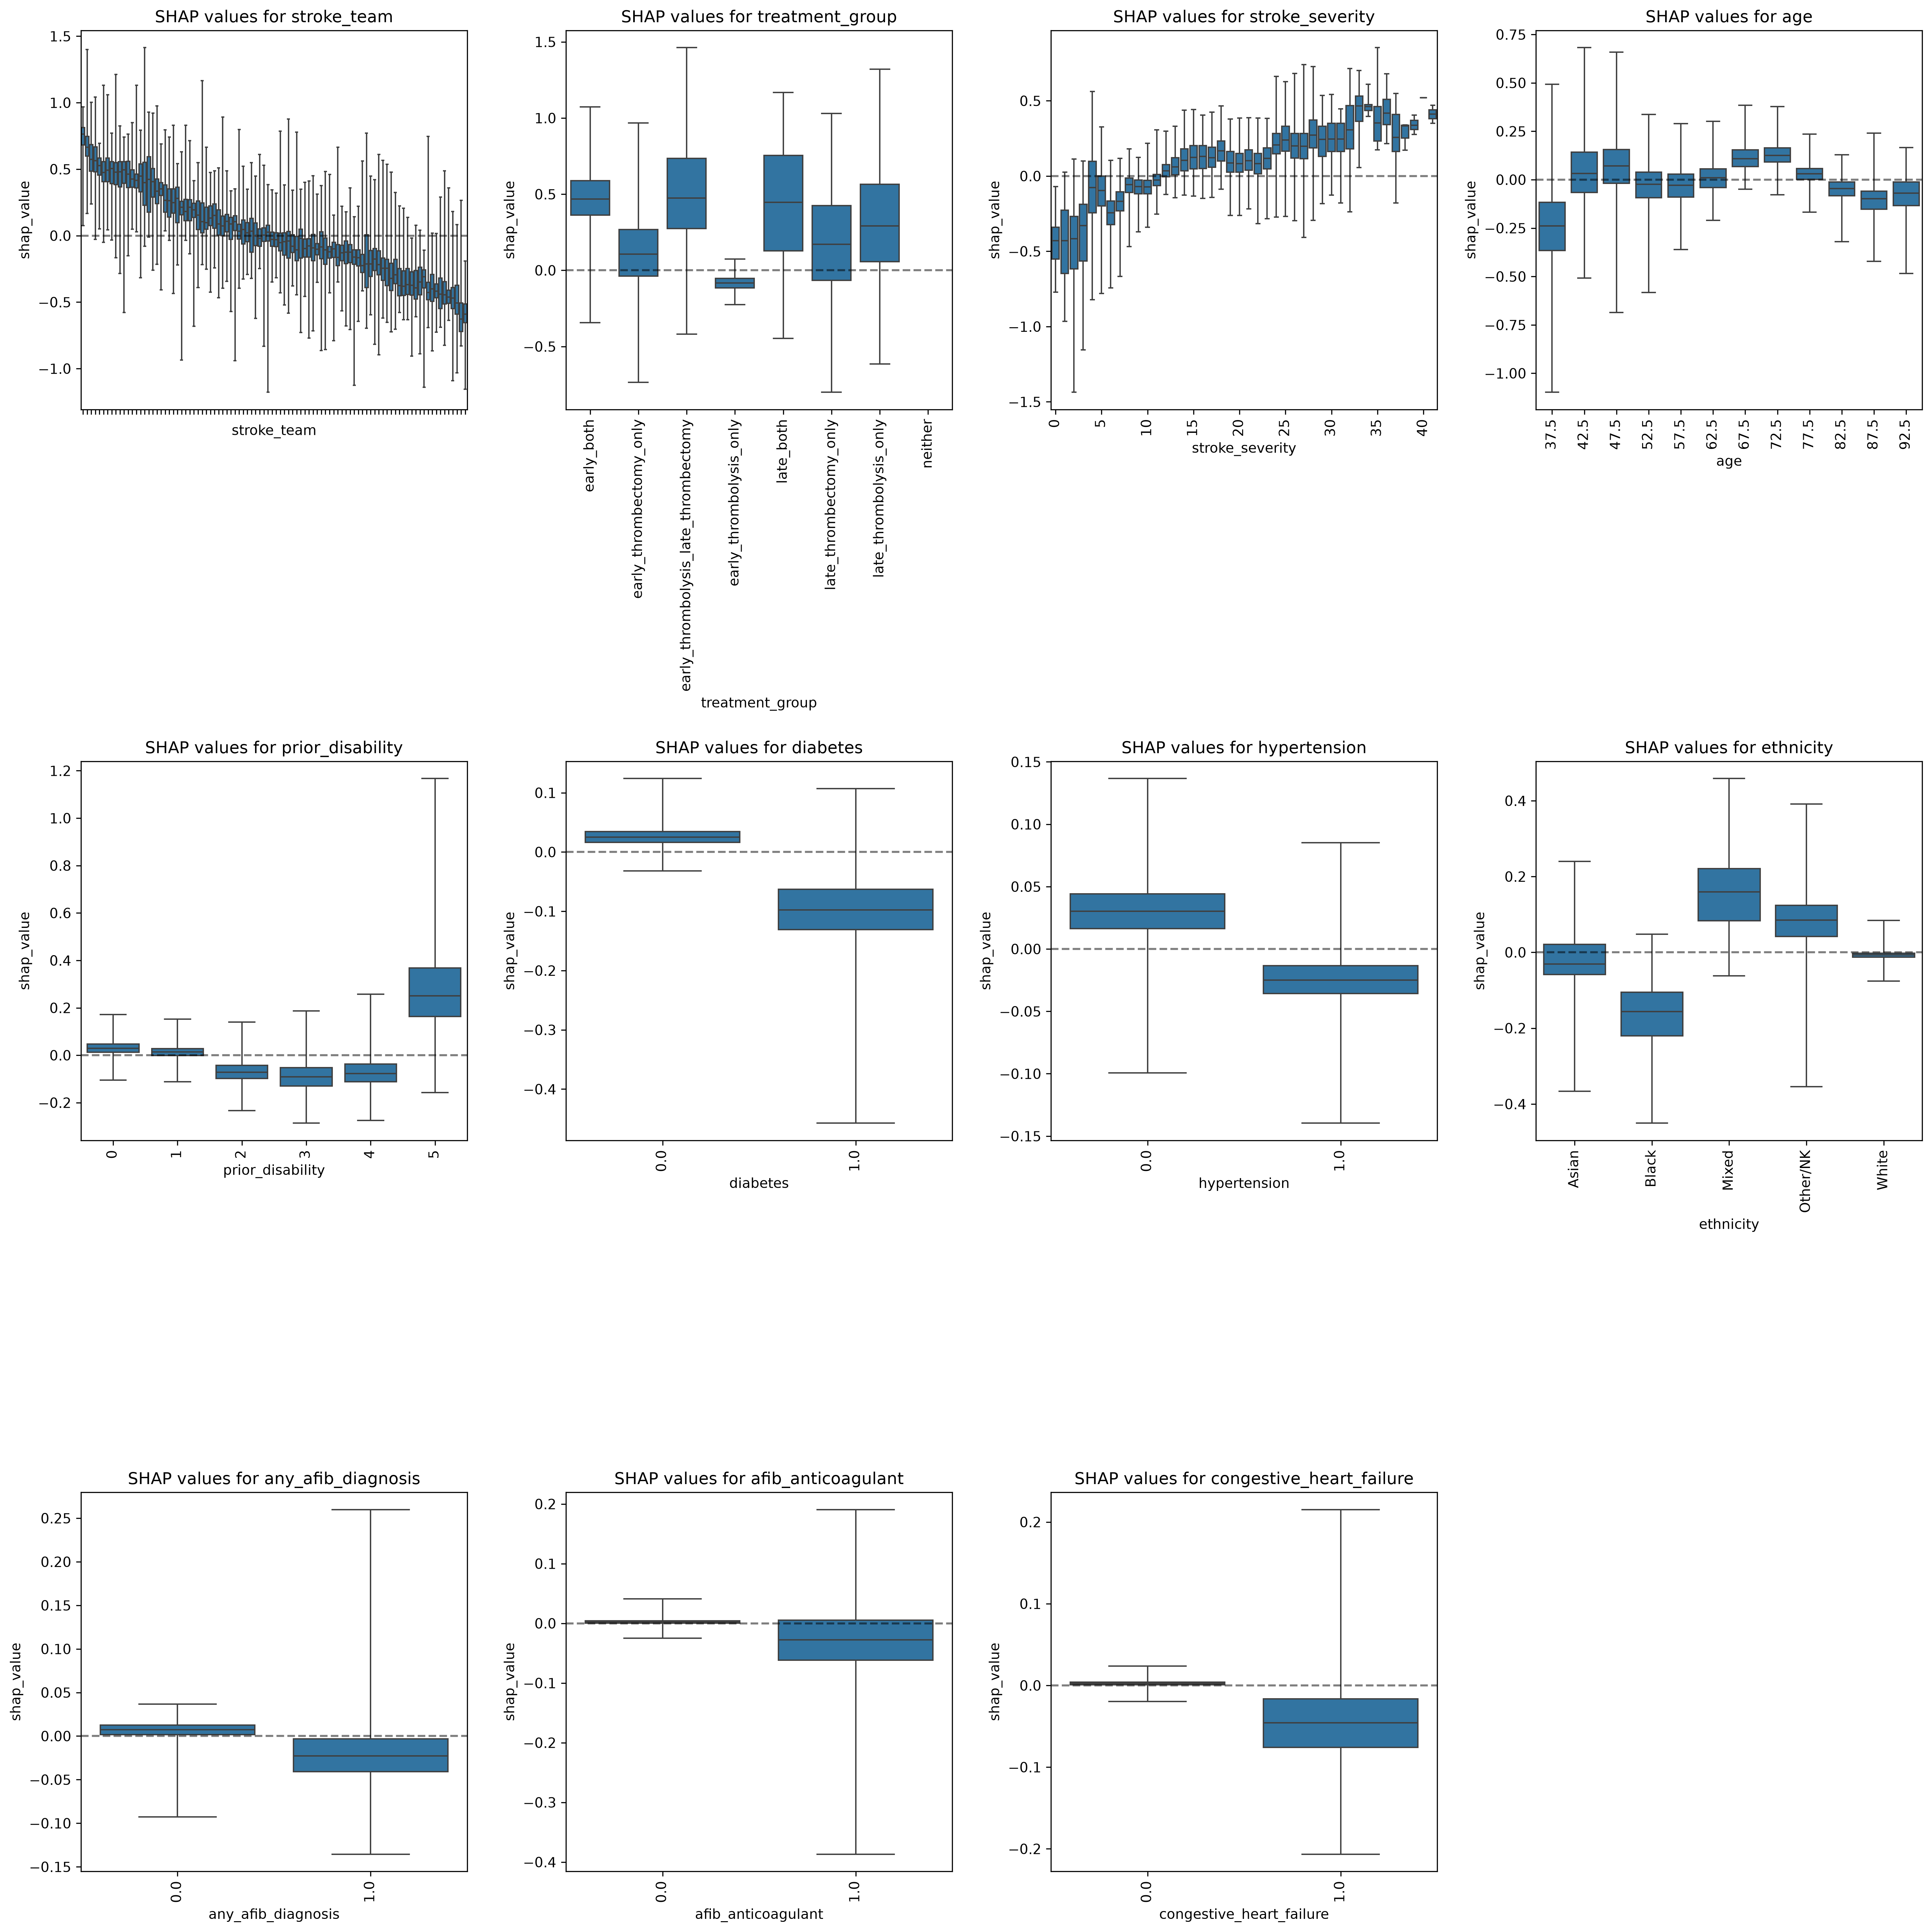
\includegraphics[width=1\linewidth]
{images/treatment_effects/s_learner_shap_box_plots_4.png}
    \caption{Effect of patient feature values on the predicted benefit of treatment. Subplots (top to bottom, left to right) are ordered by their average effect on benefit of treatment. Each subplot shows the feature value, and a boxplot of SHAP values for that feature value. The SHAP value is the contribution to the log-odds ratio treatment effect (treated vs untreated) for achieving a good outcome at the mRS 0–4 threshold.}
    \label{fig:s_learner_benefit_shap_mrs_4}
\end{figure}

\begin{figure}
    \centering
    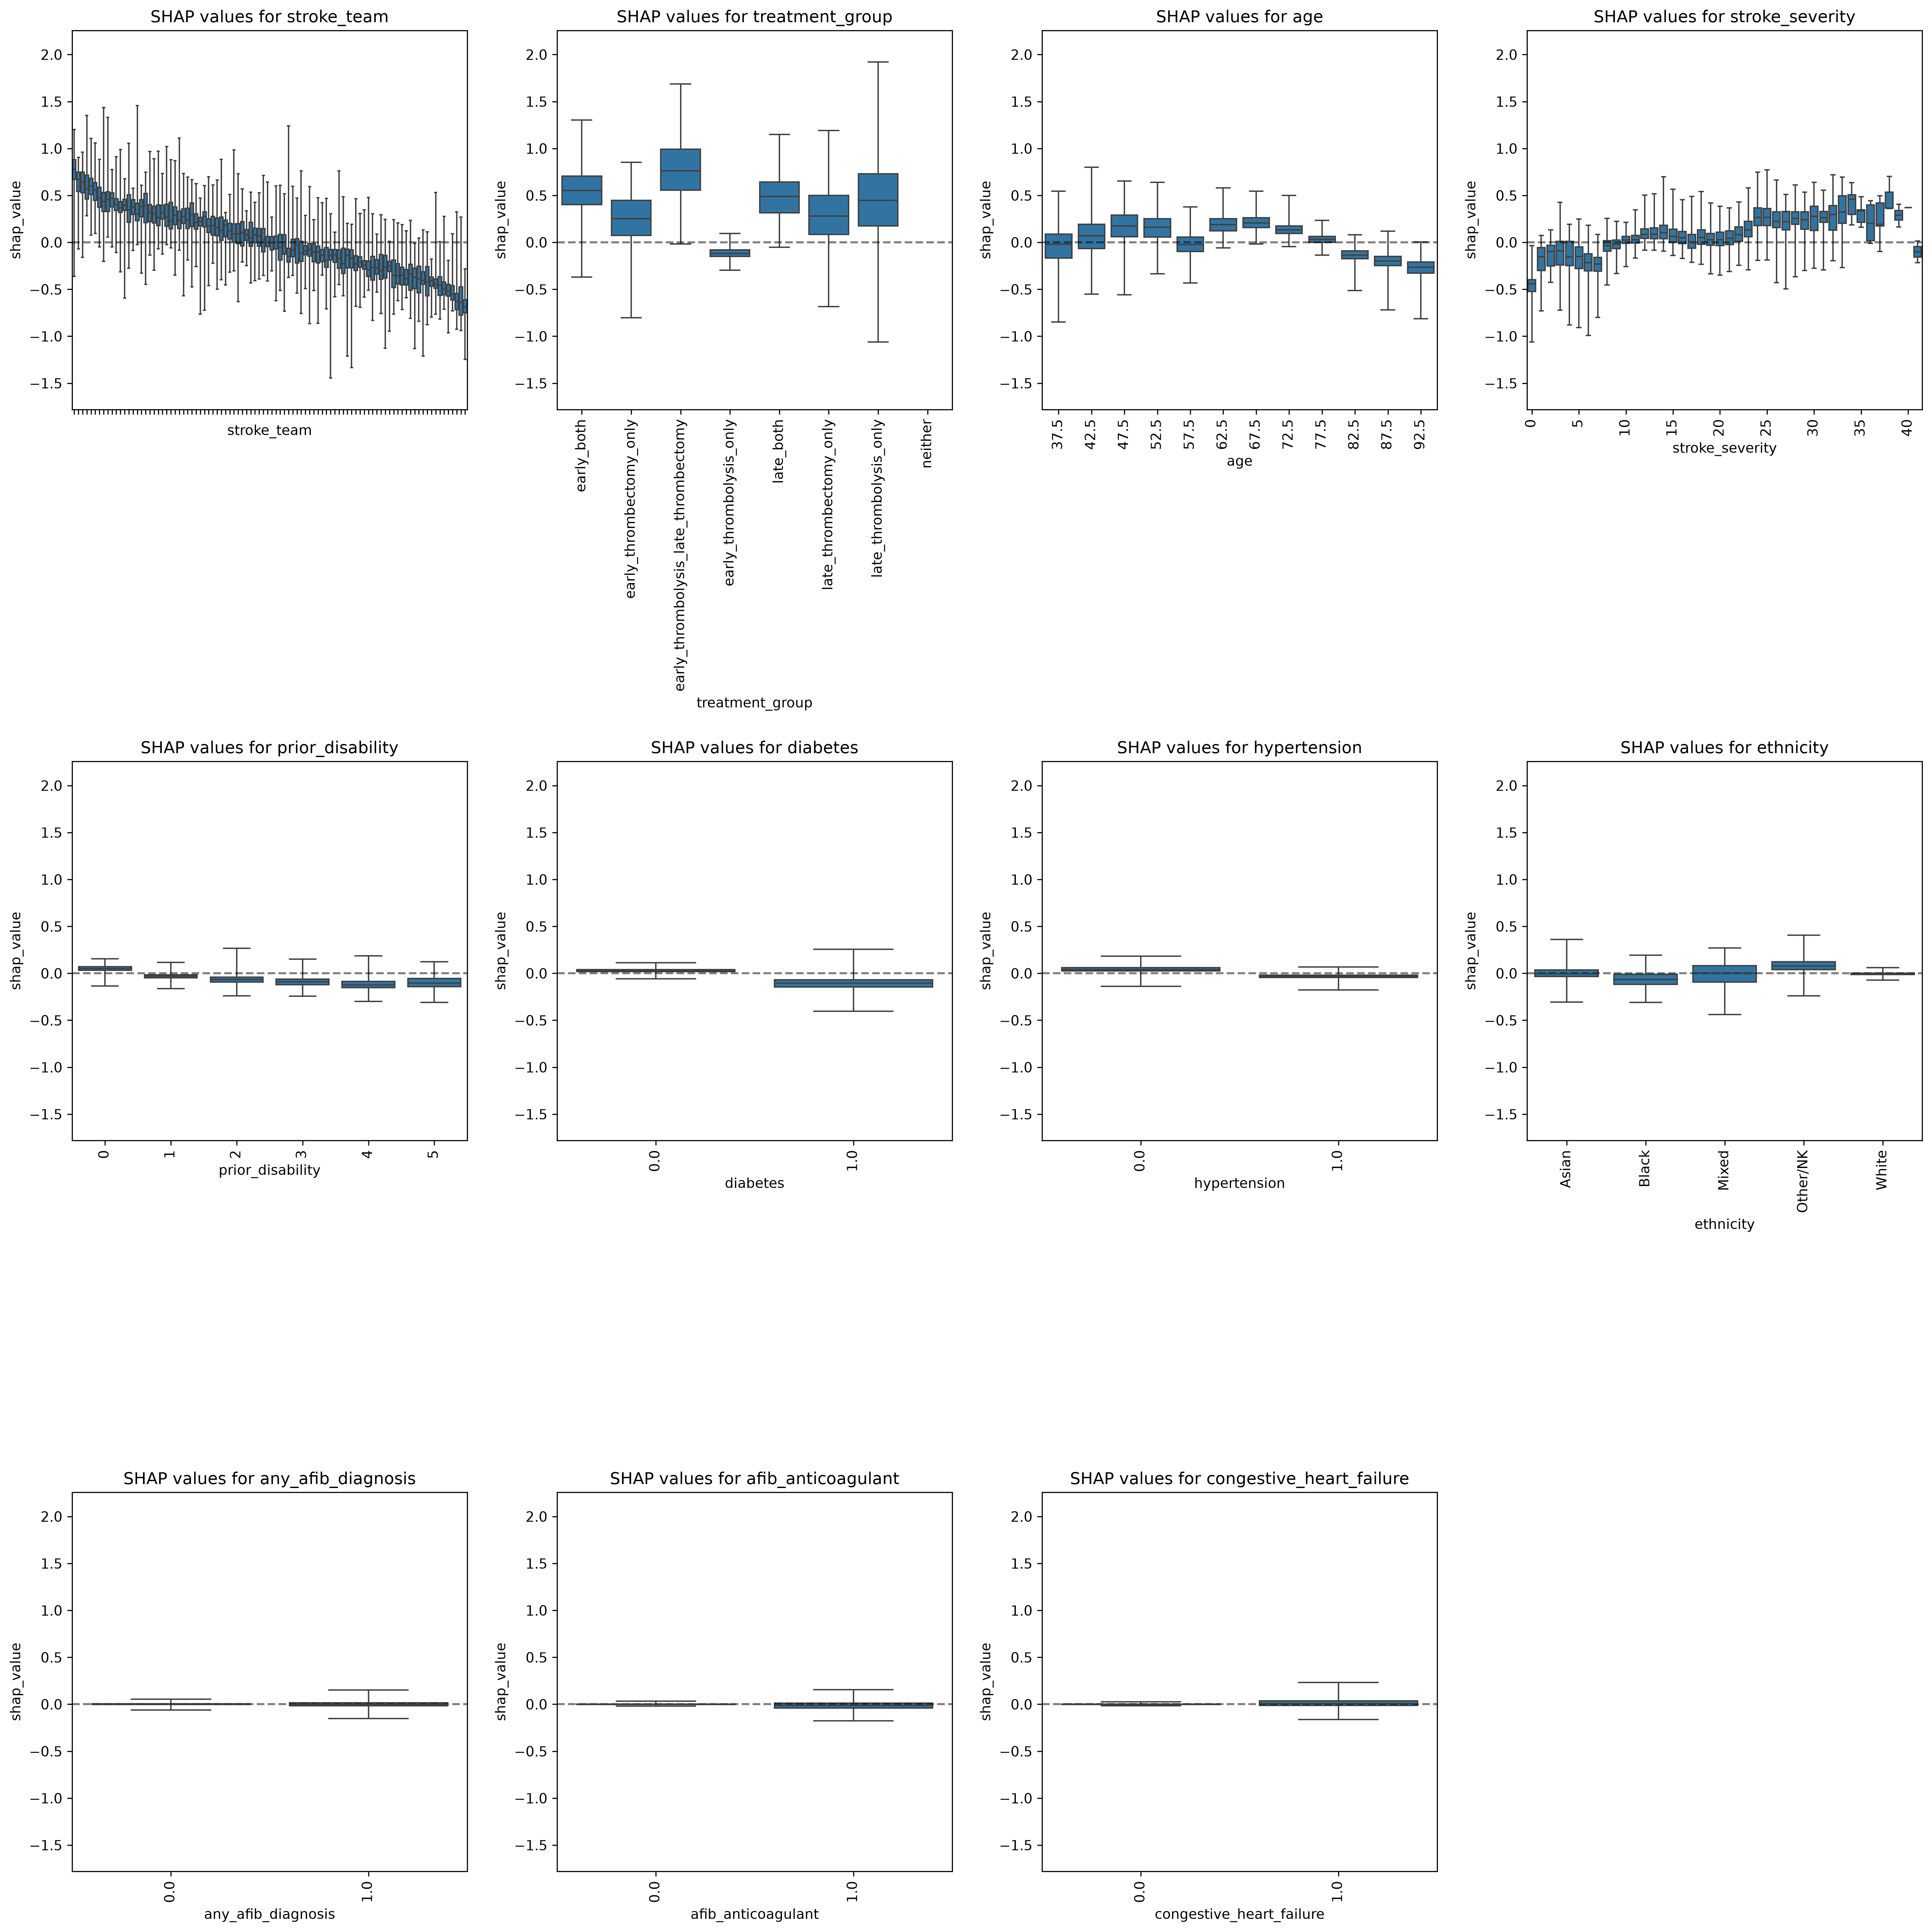
\includegraphics[width=1\linewidth]
{images/treatment_effects/s_learner_shap_box_plots_5.png}
    \caption{Effect of patient feature values on the predicted benefit of treatment. Subplots (top to bottom, left to right) are ordered by their average effect on benefit of treatment. Each subplot shows the feature value, and a boxplot of SHAP values for that feature value. The SHAP value is the contribution to the log-odds ratio treatment effect (treated vs untreated) for achieving a good outcome at the mRS 0–5 threshold.}
    \label{fig:s_learner_benefit_shap_mrs_5}
\end{figure}







% ################### CASUAL FOREST ###########################

\newpage

\subsection{Causal Forest}

Figure \ref{fig:causal_forest_benefit} shows treatment effects estimated by the orthogonal causal forest for each mRS threshold. Treatment effects are shown as conditional average treatment effects (CATE), i.e.\ the absolute change, in percentage points, in the probability of achieving the outcome with treatment compared with no reperfusion treatment, averaged over patients in each treatment group. Unlike the S-learner, which reports effects on the log-odds scale, the causal forest reports effects on the absolute probability scale, which is directly comparable with the differences in proportions from the target trial emulation. Positive values indicate that treatment increased the probability of a good outcome at that threshold, and horizontal bars show 95\% confidence intervals. Treatment type and timing (early vs.\ late, using a 270-minute onset-to-treatment threshold) were coded as a single categorical feature for this model.

\begin{figure}
    \centering
    
    % Top left
    \begin{subfigure}{0.49\textwidth}
        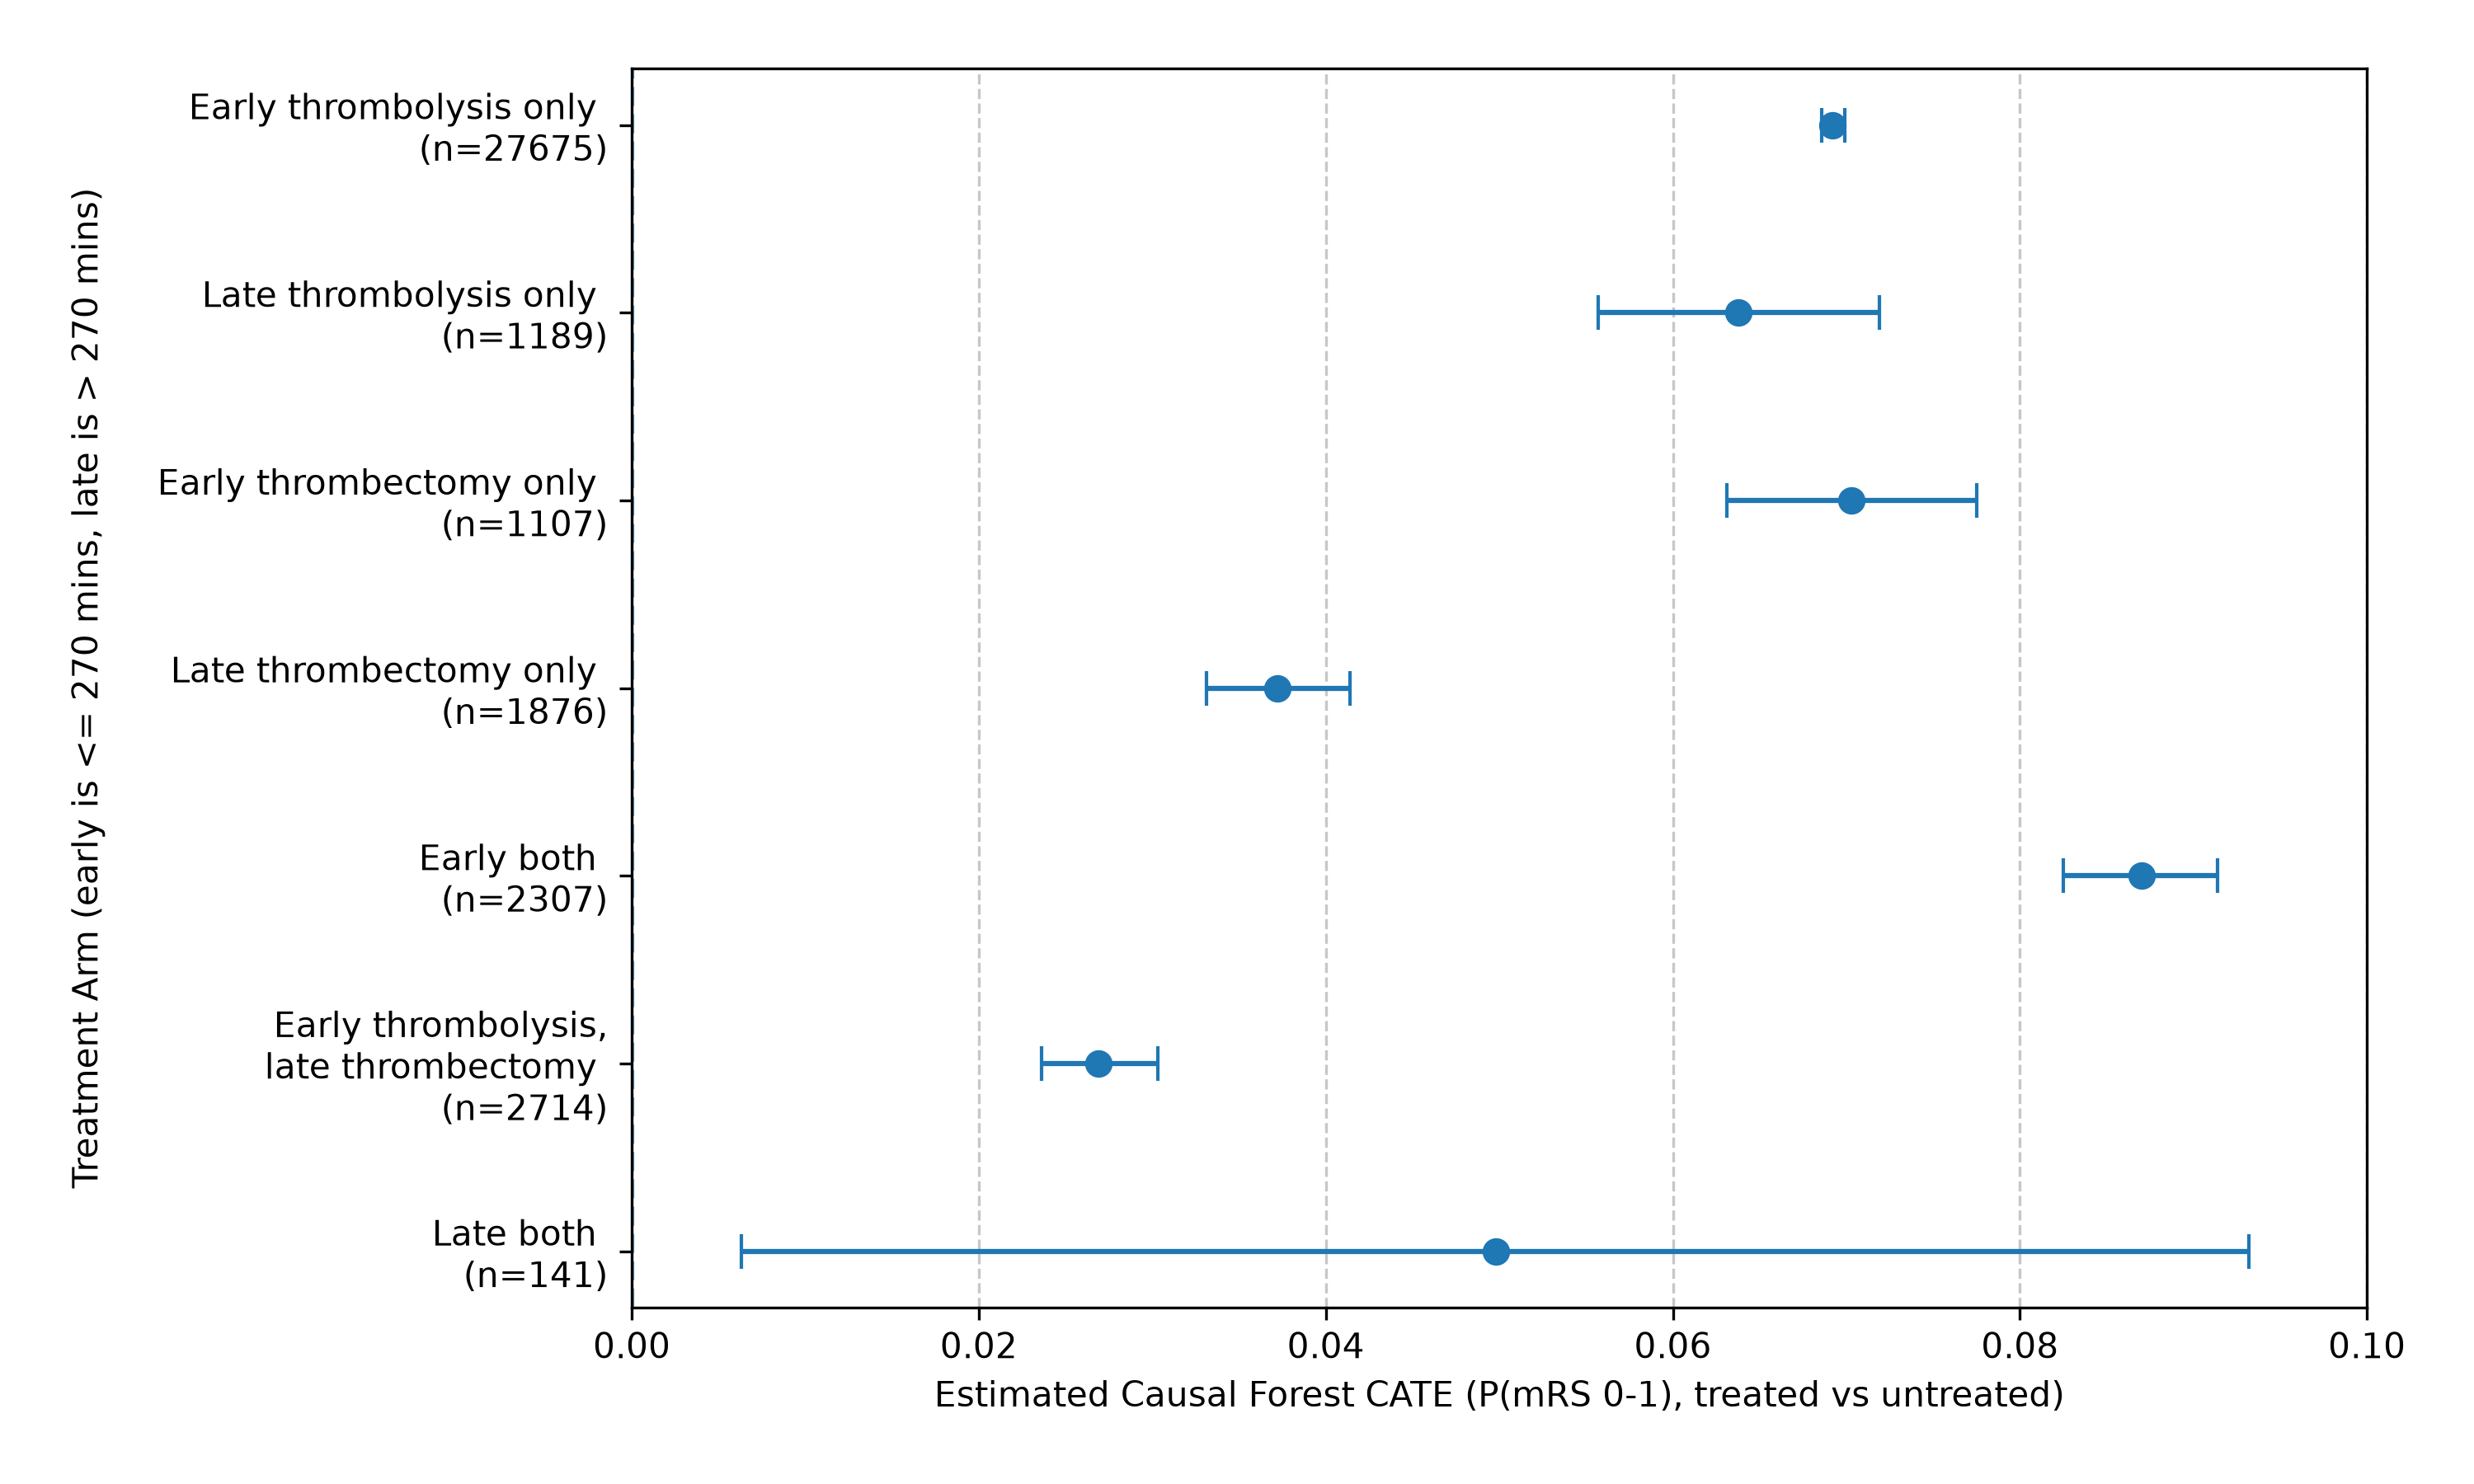
\includegraphics[width=\linewidth]{images/treatment_effects/causal_forest_counterfactual_cate_estimates_1.png}
        %\caption{}
    \end{subfigure}
    \hfill % Adds flexible horizontal spacing
    % top right image 
    \begin{subfigure}{0.49\textwidth}
        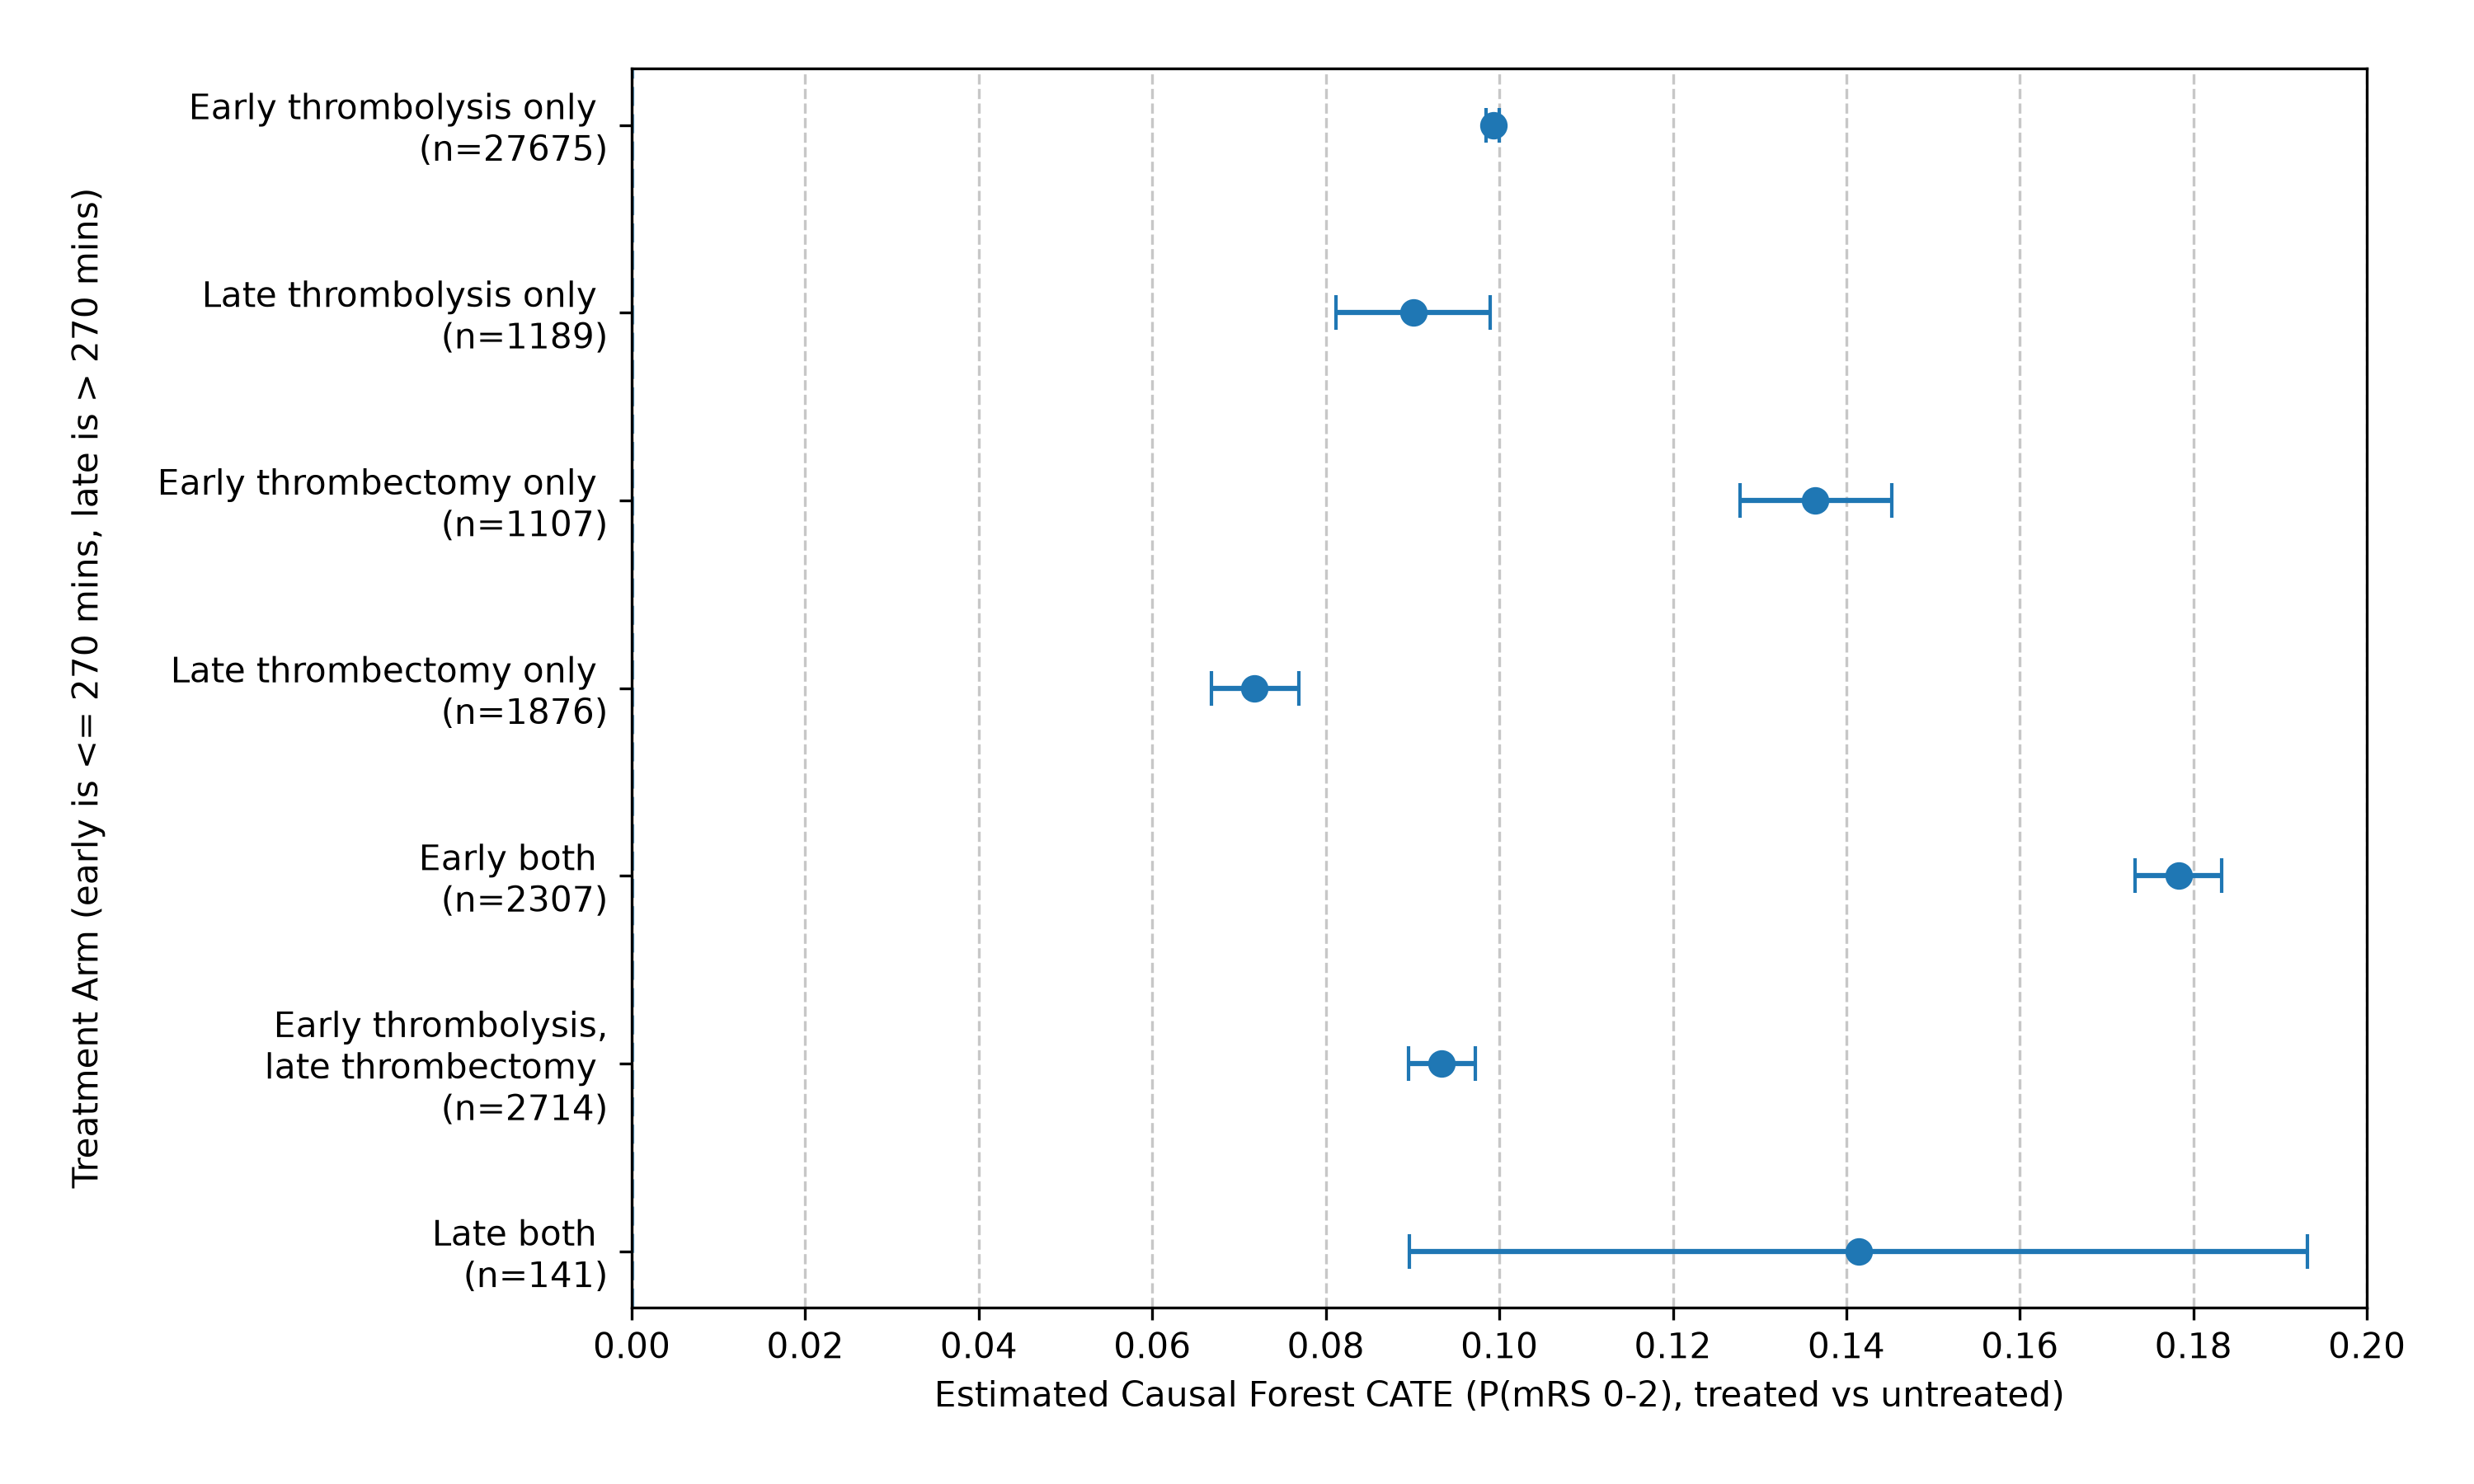
\includegraphics[width=\linewidth]{images/treatment_effects/causal_forest_counterfactual_cate_estimates_2.png}
        %\caption{}
    \end{subfigure}

    \vspace{0.5cm} % Optional vertical space between rows

    % Center left image
    \begin{subfigure}{0.49\textwidth}
        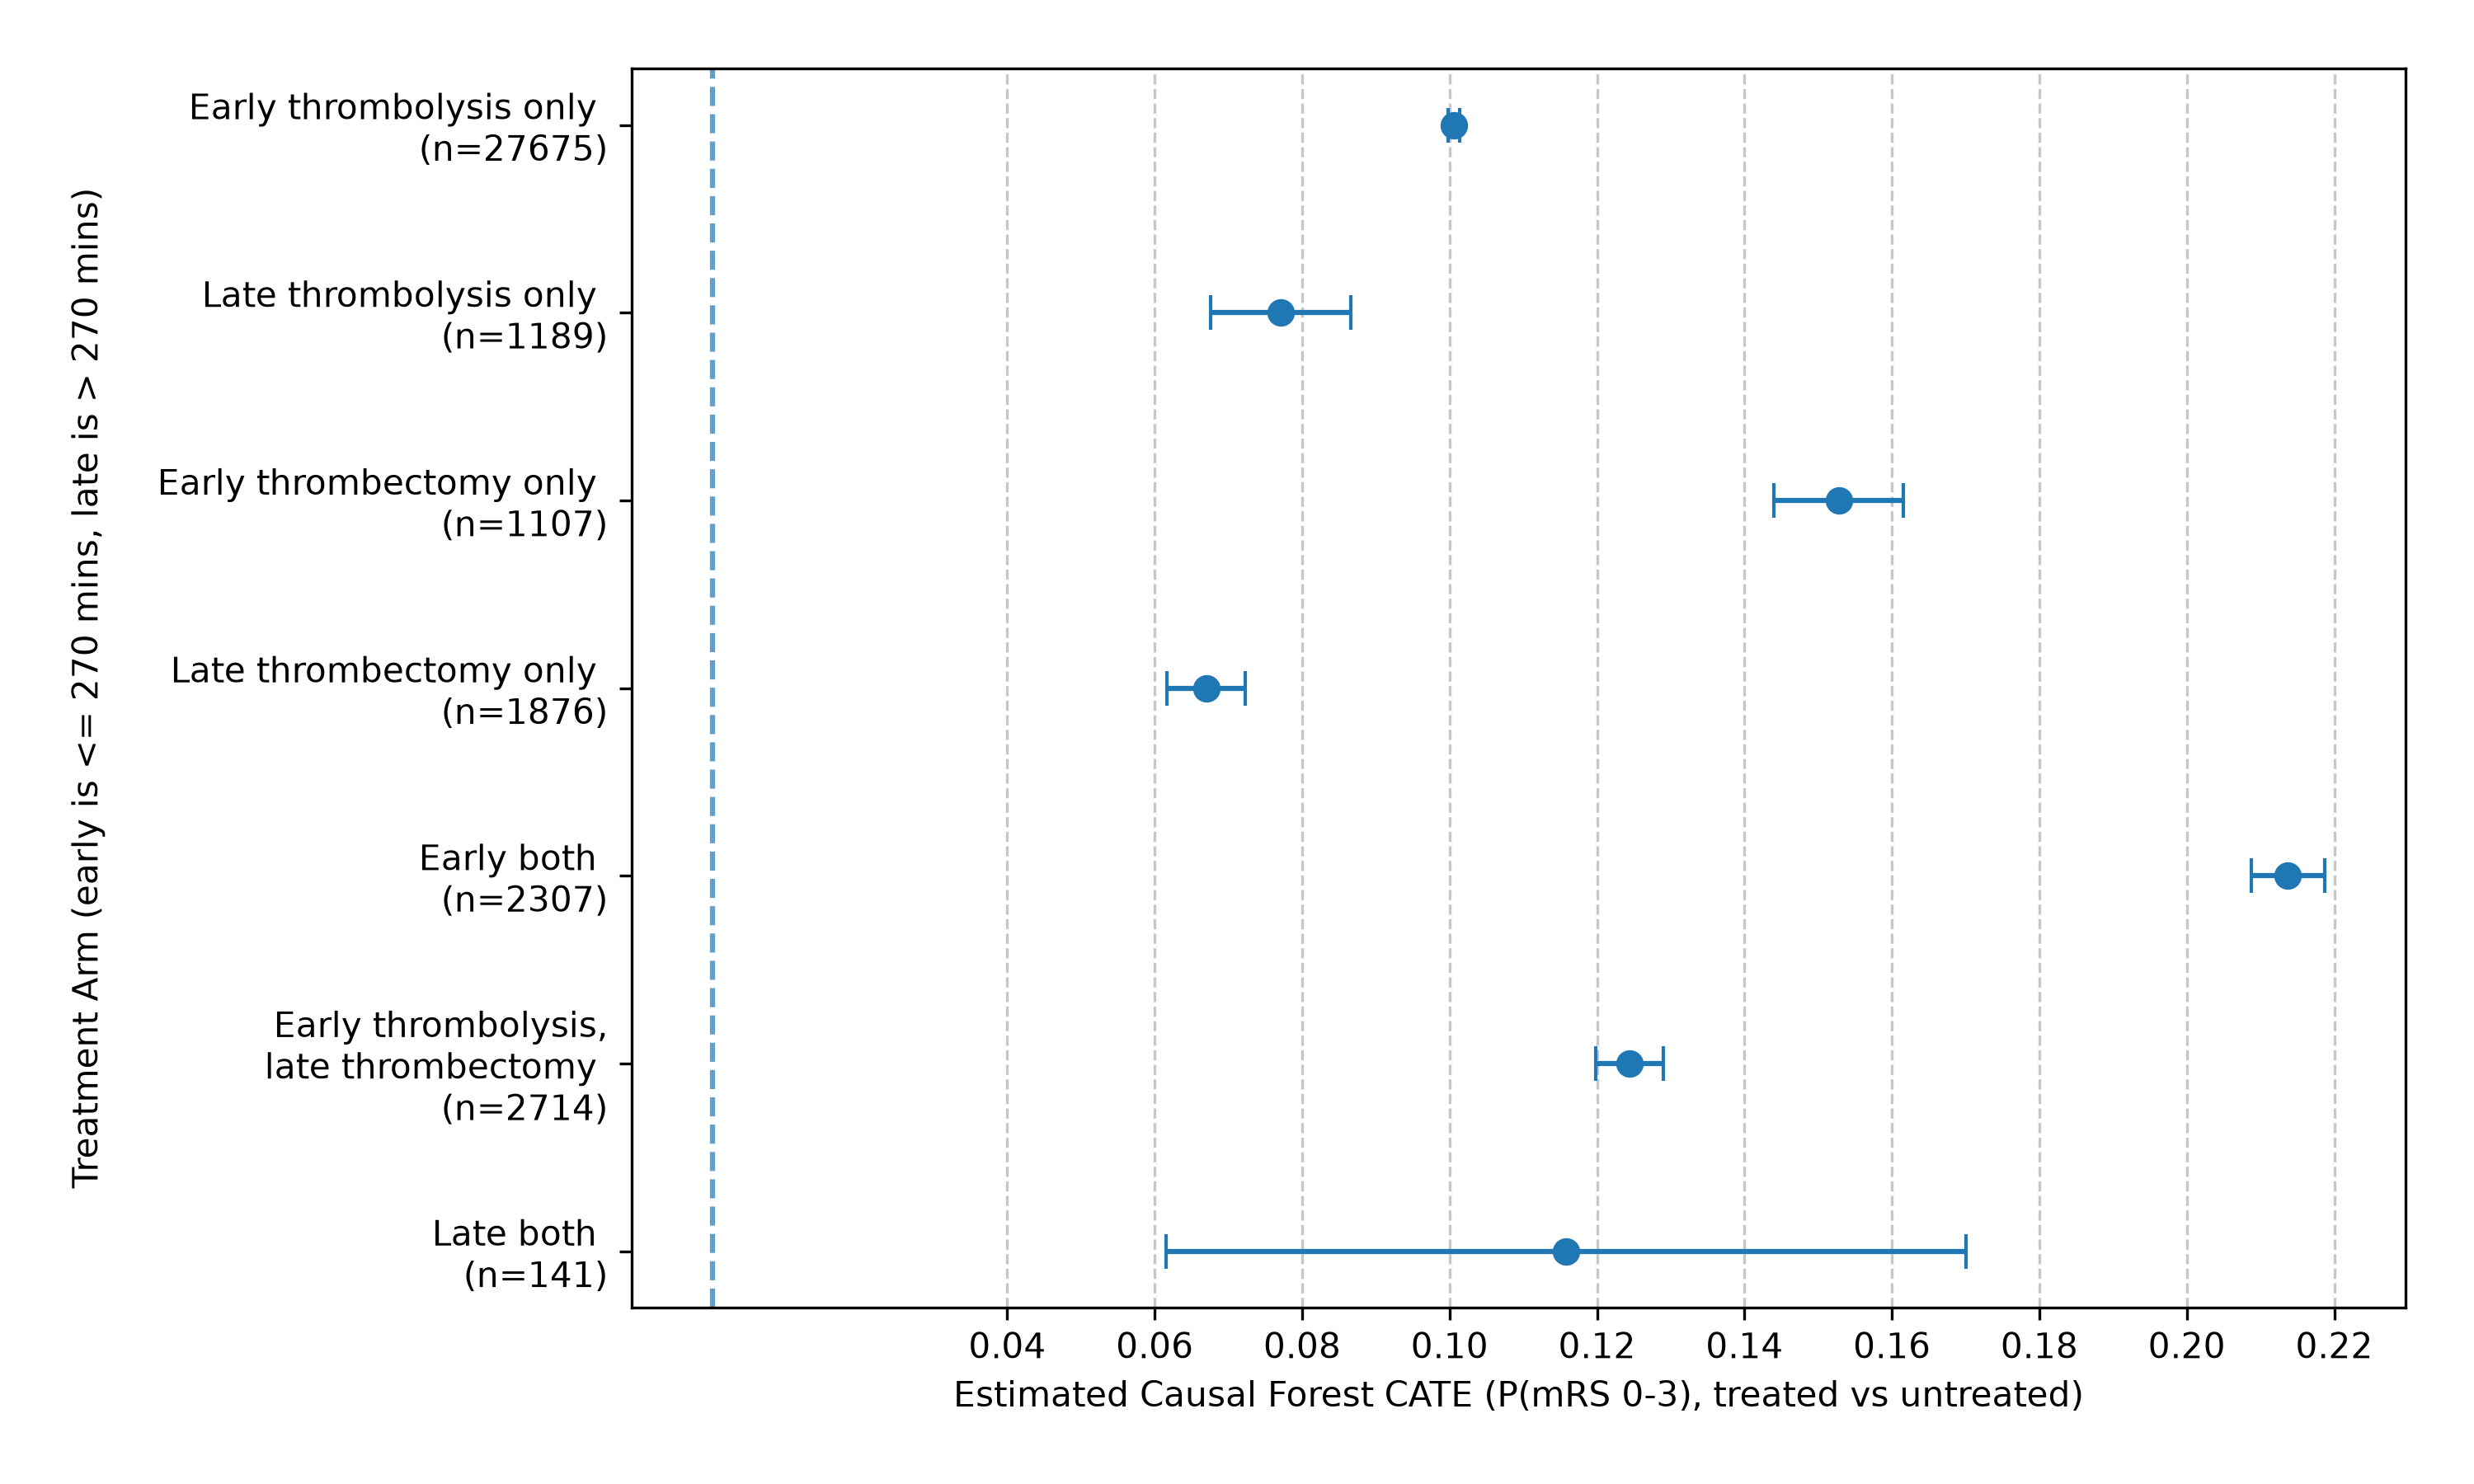
\includegraphics[width=\linewidth]{images/treatment_effects/causal_forest_counterfactual_cate_estimates_3.png}
        %\caption{}
    \end{subfigure}
    \hfill % Adds flexible horizontal spacing
    % Centre right image 
    \begin{subfigure}{0.49\textwidth}
        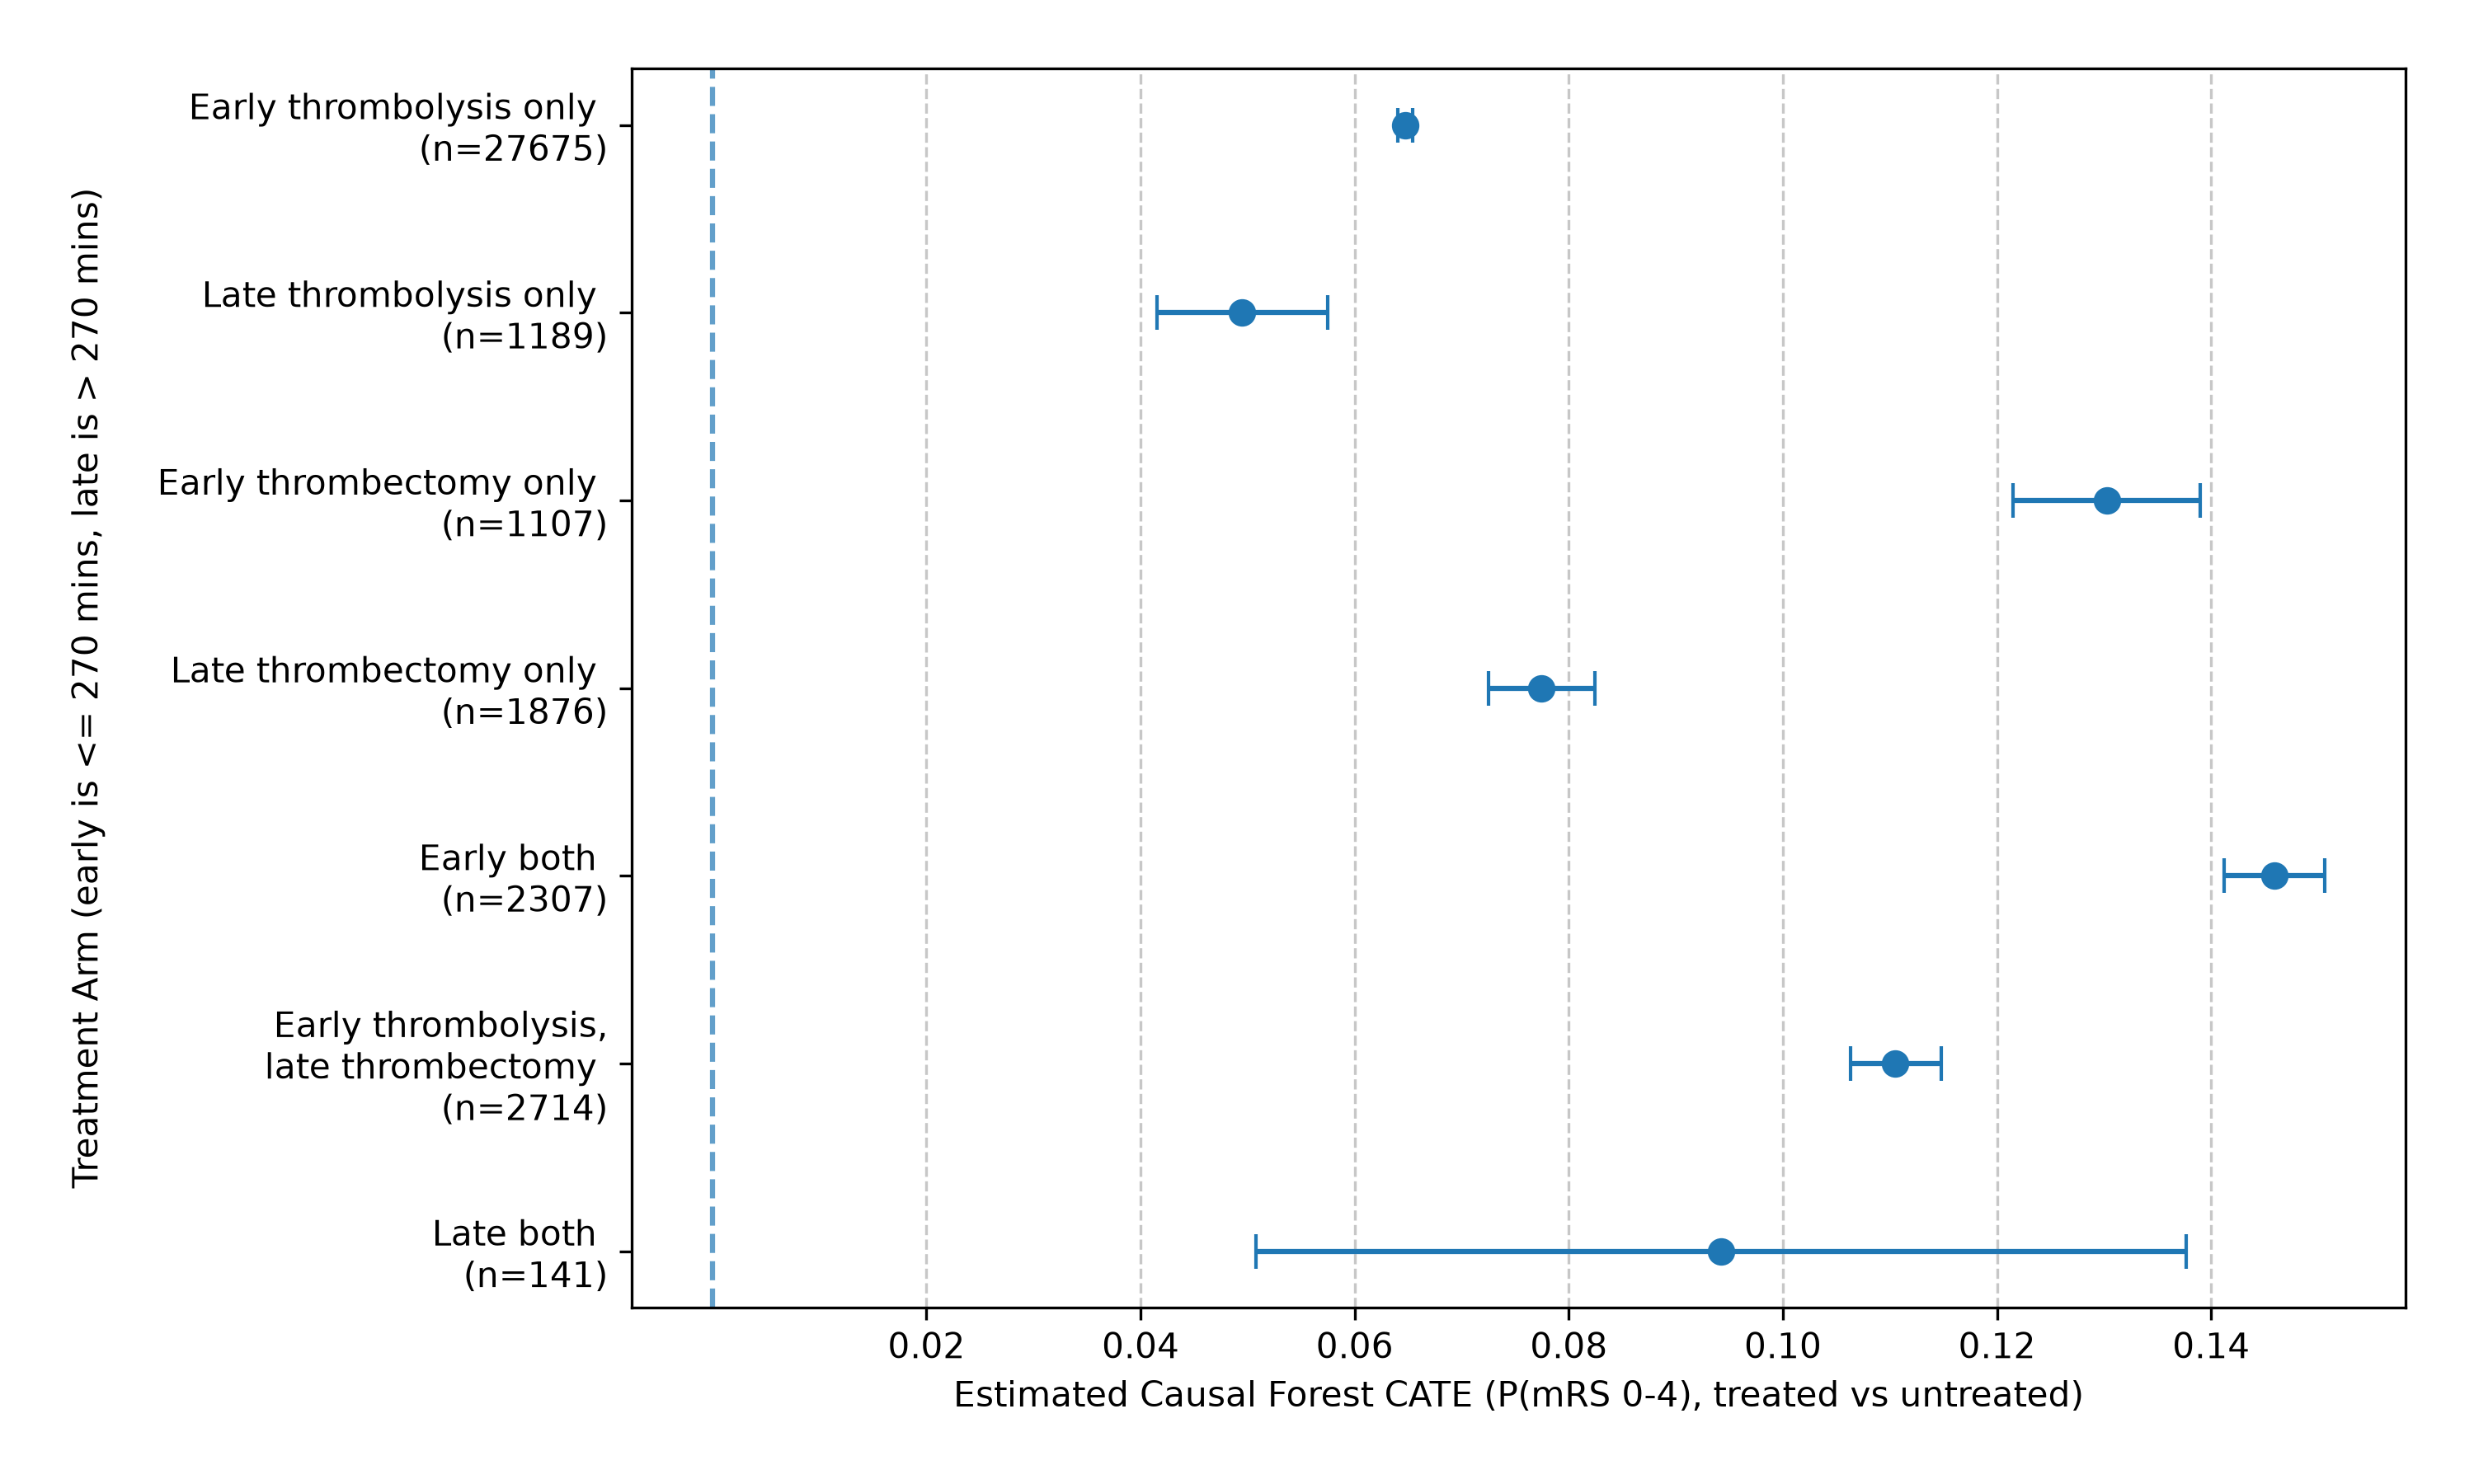
\includegraphics[width=\linewidth]{images/treatment_effects/causal_forest_counterfactual_cate_estimates_4}
        %\caption{}
    \end{subfigure}

    \vspace{0.5cm} % Optional vertical space between rows

    % Bottom image
    \begin{subfigure}{0.49\textwidth}
        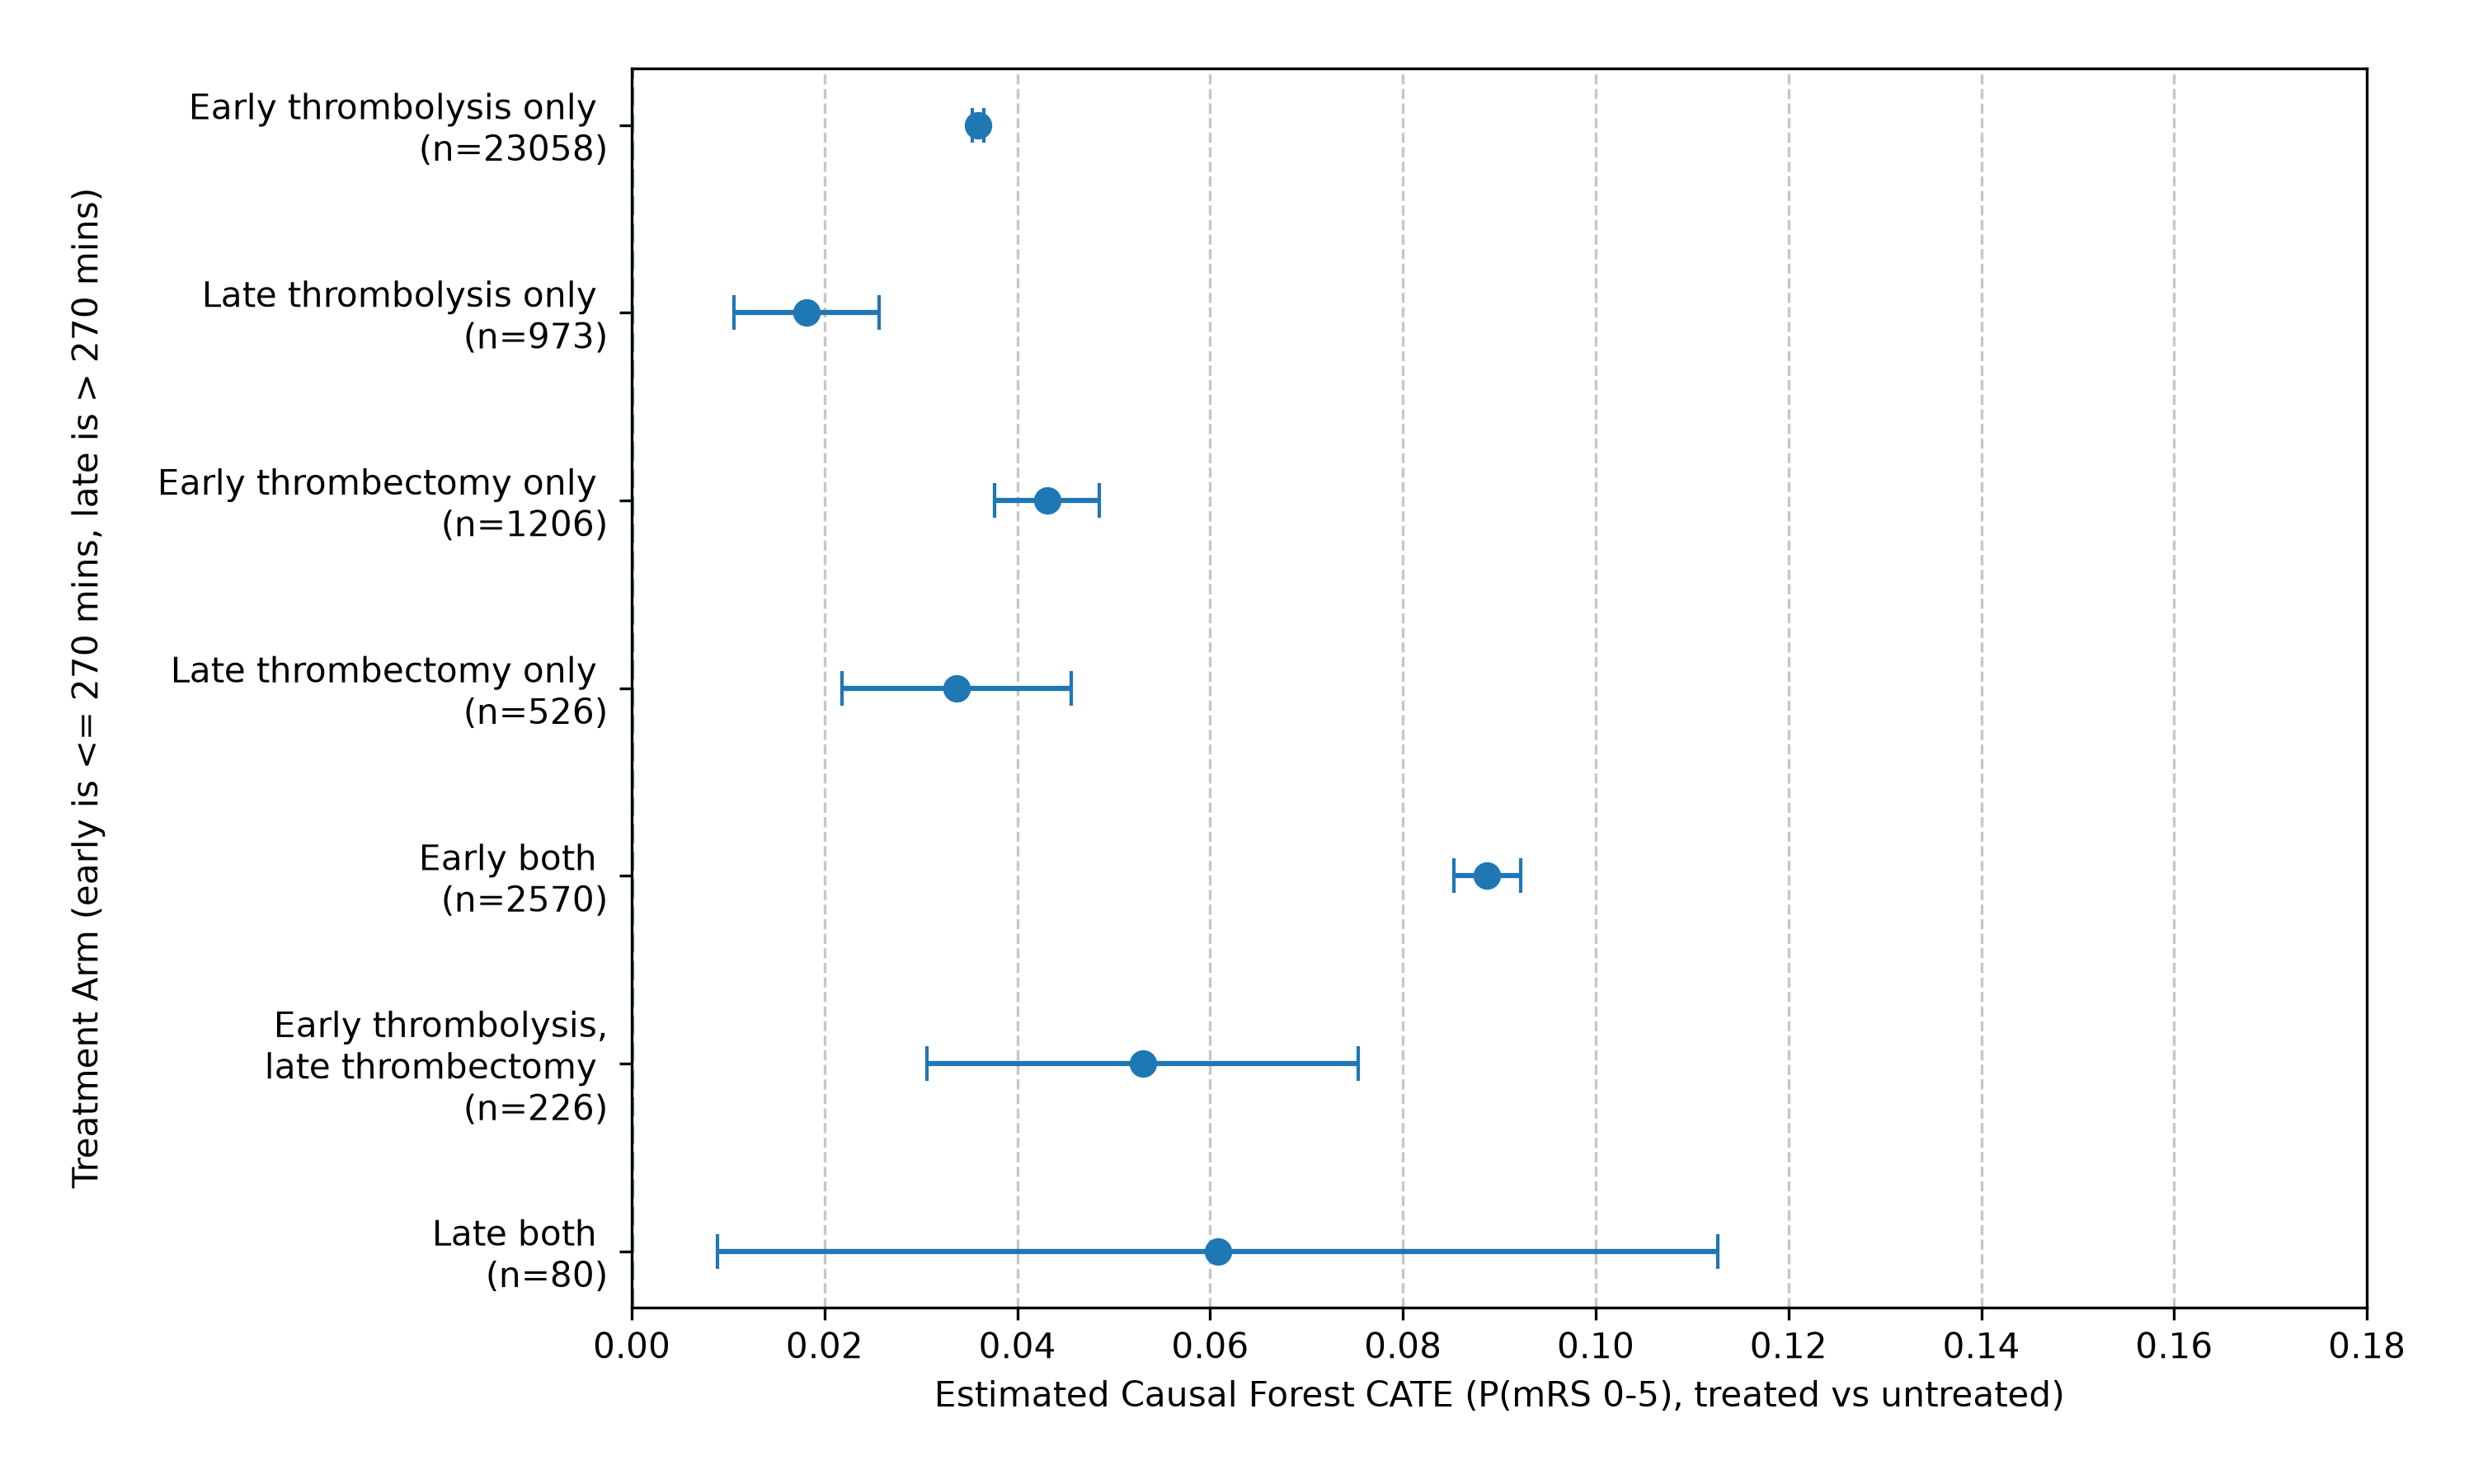
\includegraphics[width=\linewidth]{images/treatment_effects/causal_forest_counterfactual_cate_estimates_5}
        %\caption{}
    \end{subfigure}
    
    \caption{Estimated counterfactual treatment benefit across reperfusion-treatment timing strategies, derived from the Causal Forest model. Each panel shows results for discharge at or below each modified Rankin Scale (mRS) level. Points represent the mean estimated individual treatment effect for each treatment-timing group, expressed as the counterfactual probability improvement for the specified outcome relative to no reperfusion treatment; horizontal error bars show 95\% confidence intervals. Treatment groups are defined by receipt of intravenous thrombolysis and/or mechanical thrombectomy, with early treatment defined as onset-to-treatment time $<$270 minutes and late treatment as $\geq$270 minutes. Sample sizes are shown alongside group labels. Values above zero indicate a model-predicted increase in the probability of a good outcome at the corresponding threshold under the observed treatment strategy compared with no treatment.}
    \label{fig:causal_forest_benefit}
\end{figure}




% Supplement-only: the supplement has its own citations, so add a reference list
\ifincludemain\else
  \bibliographystyle{naturemag}
  \bibliography{references}
\fi

\fi


% Word counts - Don't count these!
%TC:ignore
%\section{Word counts}
%\detailtexcount{main}
%TC:endignore

\end{document}
